\documentclass[12pt, a4paper, zihao=-4, openright]{ctexrep}

% 1. 字体设置：中文宋体，西文 Times New Roman
\usepackage{newtxtext} 
%\usepackage[UTF8, fontset=windows]{ctex} 

% 2. 页面设置：A4幅面，常规边距
\usepackage[a4paper, top=2.54cm, bottom=2.54cm, left=2.54cm, right=2.54cm]{geometry}

% 3. 页眉页脚与双线设置
\usepackage{fancyhdr}
%\pagestyle{fancy}
%\fancyhf{} 
%\fancyhead[C]{\leftmark} 
%%\renewcommand{\headrule}{\vspace{-0.4pt}\hrule height 1.5pt width \headwidth \vspace{-1.2pt}\hrule height 0.5pt width \headwidth}
%\fancyfoot[C]{\thepage}       


% 3. 设置常规的 fancy 样式
\pagestyle{fancy}
\fancyhf{} % 清除默认设置
\fancyhead[C]{\leftmark} % 居中显示章标题
\fancyfoot[C]{\thepage} % 居中显示页码

% 自定义双线页眉
\renewcommand{\headrule}{%
	\vspace{-0.4pt}\hrule height 1.5pt width \headwidth 
	\vspace{-1.2pt}\hrule height 0.5pt width \headwidth
}

% 2. 关键步骤：重新定义 plain 样式，使其与 fancy 保持一致
\fancypagestyle{plain}{%
	\fancyhf{} % 清除 plain 样式的默认设置
	\fancyhead[C]{\leftmark} % 让章标题页也显示居中的章标题
	\fancyfoot[C]{\thepage} % 让章标题页也显示居中的页码
	\renewcommand{\headrule}{% % 让章标题页也有双线页眉
		\vspace{-0.4pt}\hrule height 1.5pt width \headwidth 
		\vspace{-1.2pt}\hrule height 0.5pt width \headwidth
	}
}

% 4. 目录超链接与PDF元数据设置
\usepackage{hyperref}
\hypersetup{
    colorlinks=true,          linkcolor=blue,        
    urlcolor=blue,         
    citecolor=green,       
    %bookmarks=true,        
    pdfstartview=FitH      
}

% 5. 章节排版控制
\usepackage{titlesec}
\titleformat{\chapter}[block]{\normalfont\huge\bfseries\centering}{第\,\thechapter\,章}{20pt}{\Huge}
\titlespacing*{\chapter}{0pt}{-10pt}{40pt}
\titleformat{\section}[block]{\normalfont\Large\bfseries\raggedright}{\thesection}{1em}{}

% 6. 其他常用宏包
\usepackage{graphicx}
\usepackage{float}         % 提供 [H]：把图片精确固定在正文位置（不浮动，避免图跑到别的页/别的段落下面）      
\usepackage{booktabs}      
\usepackage{amsmath,amssymb,bm}       
\usepackage{caption}       
\usepackage{setspace}      
\onehalfspacing 

\usepackage{tikz}
\usetikzlibrary{shapes.geometric, arrows.meta,calc} % 几何图形、箭头样式
% 定义节点样式
\tikzstyle{startstop} = [rectangle, rounded corners, minimum width=3cm, minimum height=1cm, text centered, draw=black, fill=white]
\tikzstyle{process}   = [rectangle, minimum width=3cm, minimum height=1cm, text centered, draw=black, fill=white]
\tikzstyle{decision}  = [diamond, aspect=3, minimum width=3cm, minimum height=1.0cm, text centered, draw=black, fill=white]
\tikzstyle{arrow}     = [thick, ->, >=stealth] % 箭头样式

% 7. 目录标题居中
\renewcommand\contentsname{\hfill 目\quad 录 \hfill}

% 8. 【新增】引入 GB/T 7714-2015 参考文献宏包
\usepackage[numbers]{gbt7714}

\usepackage{subfig}  %替代 subfigure，插入子图

\usepackage{multirow}  % 画出有单元合并的表格

\usepackage{footmisc} % 推荐加载此宏包以获得更好脚注效果

\usepackage{tabularx}   % 自适应列宽宏包

\usepackage{siunitx} %用于自定义inch的缩写



% 1. 重命名 \paragraph 为 \subsubsubsection
\newcommand{\subsubsubsection}[1]{\paragraph{#1}\mbox{}\\}

% 2. 设置章节编号深度为3（包含 subsubsubsection）
\setcounter{secnumdepth}{3}

% 3. 设置目录显示深度为3（subsubsubsection 不出现在目录中）
\setcounter{tocdepth}{3}

\newcommand{\inch}{\,\text{''}} %自定义inch的双撇

\newcolumntype{C}{>{\centering\arraybackslash}X}



\begin{document}

% === 封面部分 ===
\begin{titlepage}
    \centering 
    \vspace*{4cm} 
    {\Huge \bfseries \textcolor{red}{9-5/8\inch 井筒深度清洁关键技术升级研究及应用} \par} 
    \vspace{2cm} 
    {\Large \textcolor{red}{井筒深度清洁工艺技术} \par} 
    \vspace{4cm} 
    {\Large \textcolor{red}{项目负责人：刘维} \par}
    \vspace{1cm}
    {\Large \textcolor{red}{承担单位：中国石油大学（北京）} \par}
    \vspace{1cm}
    {\Large \textcolor{red}{2026年9月16日} \par}
\end{titlepage}

% === 目录部分 ===
\clearpage
\pagenumbering{Roman} 
\tableofcontents

% === 正文部分 ===
\clearpage
\pagenumbering{arabic} 
\setcounter{page}{1}   


% --- 第一章 ---
%\chapter{砂砾、铁屑、结垢物、蜡等井筒内的运移及分布规律研究}
	%% !TeX root = ../../main.tex

\label{keliyunyi}
在修井作业过程中，井筒内原有颗粒物以及作业过程中产生的新生颗粒物会显著影响井筒工况。颗粒物的存在不仅可能降低井下工具的工作效率，还可能诱发卡钻等重大安全事故。颗粒在井筒内的悬浮状态及运移特性受多种因素共同影响，主要包括颗粒粒径与密度、井眼尺寸与井斜角度，以及洗井液密度、粘度和流速等。本章基于流体动力学与颗粒动力学理论，针对砂砾、铁屑、结垢物和蜡质等典型颗粒物在井筒内的运移规律开展系统研究。通过构建Fluent与EDEM双向耦合仿真模型，定量分析流体参数（流速、粘度）和井筒结构参数（井斜角度）对固体颗粒运移轨迹、沉积速率及空间分布特征的影响规律。

本章仿真方案的具体实施步骤如下：首先，构建颗粒物模型并设置相关参数，基于EDEM平台按照实际物理尺寸完成颗粒注入；其次，构建三维井筒、管柱及环空的几何模型，在Fluent中建立流体仿真模型，设置流体域边界条件；随后，建立Fluent与EDEM之间的双向耦合接口，模拟真实井筒工况下流速、粘度等关键参数对颗粒物运移轨迹、沉积速率及空间分布特征的影响，具体操作流程如图\ref{fig:flowchart}所示；最后，利用后处理模块对仿真结果进行定量分析，包括颗粒分布统计和动力学参数提取。
    \begin{figure}[htbp]
        \centering
        \begin{tikzpicture}[node distance=2cm] % 节点间距为2cm
            % 1. 流场初始化（起始节点）
            \node (init) [startstop] {流场初始化};
            % 2. 连续相流场计算（处理节点）
            \node (flow) [process, below of=init] {连续相流场计算};
            % 3. 颗粒模型注入（处理节点）
            \node (inject) [process, below of=flow] {颗粒模型注入};
            % 4. 颗粒时间步长计算（处理节点）
            \node (time1) [process, below of=inject] {颗粒时间步长计算};
            % 6. 颗粒轨迹计算（处理节点）
            \node (trajectory) [process, below of=time1] {颗粒轨迹计算};
            % 7. 更新连续相源项（处理节点）
            \node (update) [process, below of=trajectory] {更新连续相源项};
            % 8. 判断是否收敛（决策节点）
            \node (converge) [decision, below of=update] {是否收敛};
            % 9. 判断是否计算完成（决策节点）
            \node (complete) [decision, below of=converge] {是否计算完成};
            % 10. 计算结果（终止节点）
            \node (result) [startstop, below of=complete] {计算结果};
            % 11. 更新下一步时间数据（右侧辅助节点）
            \node (nextstep) [process, right of=complete, xshift=4cm] {更新下一步时间数据};

            % 绘制箭头连线
            \draw [arrow] (init) -- (flow);                          % 流场初始化 → 连续相流场计算
            \draw [arrow] (flow) -- (inject);                        % 连续相流场计算 → 颗粒模型注入
            \draw [arrow] (inject) -- (time1);                       % 颗粒模型注入 → 颗粒时间步长计算
            \draw [arrow] (time1) -- (trajectory);                   % 颗粒时间步长计算 → 颗粒轨迹计算
            \draw [arrow] (trajectory) -- (update);                  % 颗粒轨迹计算 → 更新连续相源项
            \draw [arrow] (update) -- (converge);                    % 更新连续相源项 → 判断是否收敛

            % 收敛判断分支（未收敛→返回连续相流场计算）
            \draw [arrow] (converge.west) -- ++(-1,0) |- (flow.west) node[midway, left] {否};

            % 收敛后→计算完成判断
            \draw [arrow] (converge) -- (complete) node [midway, right] {是};

            % 计算完成判断分支（未完成→更新下一步时间数据→返回连续相流场计算）
            \draw [arrow] (complete.east) -- (nextstep.west) node[midway, above] {否};
            \draw [arrow] (nextstep.north) |- (flow.east);

            % 计算完成→输出结果
            \draw [arrow] (complete) -- (result) node[midway, right] {是};
        \end{tikzpicture}
        \caption{颗粒运移模型计算流程图}
        \label{fig:flowchart}  
    \end{figure}

\section{基本理论和模拟条件}  
\subsection{EDEM理论基础} 
井筒中的颗粒在运移过程中产生颗粒-颗粒、颗粒-管壁之间的接触是不可避免的，该过程将产生作用力，本文采用EDEM软件进行模拟。EDEM软件的理论基础是离散元法（Discrete Element Method, DEM），DEM对上述两种接触对进行建模，求解接触中颗粒所受外力作用以及力矩。根据工况的不同，可区分干颗粒和湿颗粒两种类型，
当计算物料为干颗粒时，接触点不存在粘结的作用，EDEM软件默认采用Hertz-Mindlin基本接触模型，颗粒接触受力模型如图\ref{fig:particle_collision}所示。
\begin{figure}[htbp]
	\centering
	\subfloat[双颗粒碰撞模型示意图]{%
		\includegraphics[width=0.45\textwidth]{figure/kelipengzhuang.png}
		\label{fig:particle_collision}
	}
	%\vspace{0pt}
	\subfloat[Hertz--Mindlin 接触模式示意图]{%
		\includegraphics[width=0.55\textwidth]{figure/hertz-mindlin-contact-model.png}
		\label{fig:hertz_mindlin_contact_model}
	}
	\caption{颗粒--颗粒碰撞建模}
	\label{fig:particle_collision_and_contact_model}
\end{figure}

% \begin{figure}[htbp]
% 	\centering
% 	\includegraphics[width=0.6\textwidth]{figure/hertzian-soft-sphere-model.png}
% 	\caption{Hertzian 软球模型}
% 	\label{fig:hertzian_soft_sphere_model}
% \end{figure}


假设发生弹性接触的两球形颗粒的半径分别为 \(R_{1}\)、\(R_{2}\)，则颗粒间产生的法向接触力大小 \(F_{\mathrm{n}}\) 的计算式为
\begin{equation}
	F_{\mathrm{n}}=\frac{4}{3}E_{\mathrm{eq}}\sqrt{R_{\mathrm{eq}}}\,\delta^{3/2}
	\label{eq:normal_particle_elastic_force}
\end{equation}
式中，\(E_{\mathrm{eq}}\) 为等效杨氏模量，$\mathrm{GPa}$；\(\delta\) 为法向重叠量，$\mathrm{mm}$；\(R_{\mathrm{eq}}\) 为等效接触半径，$\mathrm{mm}$。\(E_{\mathrm{eq}}\) 和 \(R_{\mathrm{eq}}\) 的计算式为
\begin{equation}
	\begin{aligned}
		E_{\mathrm{eq}} & = \left(\frac{1 - \nu_1^2}{E_1} + \frac{1 - \nu_2^2}{E_2} \right)^{-1}\\
	R_{\mathrm{eq}} & =\left(\frac{1}{R_{1}}+\frac{1}{R_{2}}\right)^{-1}
	\end{aligned}
\end{equation}
式中，\(E_{1}\)、\(E_{2}\) 分别为颗粒1、2 的杨氏模量，$\mathrm{GPa}$；\( \nu_{1} \)、\( \nu_{2} \) 分别为颗粒 1、2 的泊松比。


颗粒间法向阻尼力 \(F_{\mathrm{n}}^{\mathrm{d}}\) 及切向阻尼力 \(F_{\mathrm{t}}^{\mathrm{d}}\) 的计算公式为
\begin{equation}
	\begin{aligned}
	F_{\mathrm{n}}^{\mathrm{d}} &= 2\sqrt{\frac{5}{6}}\beta\sqrt{S_{\mathrm{n}}m_{\mathrm{eq}}}\,v_{\mathrm{n}}^{\mathrm{rel}}\\
	F_{\mathrm{t}}^{\mathrm{d}} &= 2\sqrt{\frac{5}{6}}\beta\sqrt{S_{\mathrm{t}}m_{\mathrm{eq}}}\,v_{\mathrm{t}}^{\mathrm{rel}}
	\end{aligned}
	\label{eq:normal_shear_damping_force}
\end{equation}
%这是Tsuji阻尼模型
式中，\(S_{\mathrm{n}}\) 为法向刚度，\(S_{\mathrm{t}}\) 为切向刚度，$\mathrm{N/m}$；\(v_{\mathrm{n}}^{\mathrm{rel}}\) 为法向真实速度，\(v_{\mathrm{t}}^{\mathrm{rel}}\) 为切向真实速度，$\mathrm{m/s}$；\(m_{\mathrm{eq}}\) 为等效质量，\(\mathrm{kg}\)；\(\beta\) 为阻尼系数。法向和切向共用同一阻尼系数\(\beta\)，与颗粒碰撞前后的恢复系数\(e\)的关系为
\begin{equation}
	\beta = \frac{\ln e}{\sqrt{\ln^2 e + \pi ^2}}
\end{equation}
%恢复系数e定义为碰撞后法向相对分离速度与碰撞前法向相对接近速度之比：e= v_接近/v_分离

等效质量\(m_\mathrm{eq}\)的计算式为
\begin{equation}
	m_{\mathrm{eq}} = \left(\frac{1}{m_{1}}+\frac{1}{m_{2}}\right)^{-1}	
\end{equation}

\(S_{\mathrm{n}}\) 和\(S_{\mathrm{t}}\)的计算式为
\begin{equation}
	\begin{aligned}
		S_{\mathrm{n}} &= 2E_{\mathrm{eq}}\sqrt{R_{\mathrm{eq}}\delta}\\
		S_{\mathrm{t}} &= 8G_{\mathrm{eq}}\sqrt{R_{\mathrm{eq}}\delta}
	\end{aligned}
\end{equation}

其中，\(G_{\mathrm{eq}}\) 为等效剪切模量，Pa，其计算公式为
\begin{equation}
	G_{\mathrm{eq}}=\left(\frac{2-\nu_{1}}{G_{1}}+\frac{2-\nu_{2}}{G_{2}}\right)^{-1}
\end{equation}
式中，\(G_{1}\)、\(G_{2}\) 分别为颗粒 1、2 的剪切模量。

假设两颗粒产生接触前的速度分别为 \(\bm{v}_{1}\)、\(\bm{v}_{2}\)，\(\bm{n}\) 为产生接触时的法向单位矢量，则
\begin{equation}
		\bm{n}=\frac{\bm{r}_{1}-\bm{r}_{2}}{\left|\bm{r}_{1}-\bm{r}_{2}\right|}
\end{equation}
进而，\(v_{\mathrm{n}}^{\mathrm{rel}}\)和\(v_{\mathrm{t}}^{\mathrm{rel}}\)的计算式为
\begin{equation}
	\begin{aligned}
	v_{\mathrm{n}}^{\mathrm{rel}} &= (\bm{v}_{1}-\bm{v}_{2})\cdot\bm{n} \\
	v_{\mathrm{t}}^{\mathrm{rel}} &= \left|(\bm{v}_{1}-\bm{v}_{2}) - v_{\mathrm{n}}^{\mathrm{rel}}\bm{n} + (\bm{\omega}_{1} \times R_1\bm{n} + \bm{\omega}_{2} \times R_2\bm{n})\right|
	\end{aligned}
\end{equation}

颗粒间的切向力 \(F_{\mathrm{t}}\) 计算式为
\begin{equation}
	F_{\mathrm{t}}=S_{\mathrm{t}}\delta_{\mathrm{t}}
	\label{eq:shear_damping_force}
\end{equation}
%切向方向：接触面没有"几何上的切向重叠"这个概念。两个球在切向方向的相对运动，本质上是接触面发生了弹性剪切变形。这个变形量无法从当前几何位置反推，只能从接触开始的那一刻起，一步步累加相对切向位移。把切向接触想象成一个弹簧-阻尼-滑块串联系统：弹簧：代表接触面的弹性剪切刚度，弹簧的伸长量就是 δt，阻尼器：代表能量耗散，滑块：代表库仑摩擦极限
%这是Mindlin理论
式中，\(\delta_{\mathrm{t}}\)表示两个颗粒的切向重叠量，在两个颗粒建立接触时为零，此后时间步内进行累积
\begin{equation}
	\delta_{\mathrm{t}}^{n+1} = \delta_{\mathrm{t}}^{n} + \Delta t \cdot {v}_\mathrm{t}^\mathrm{rel}
\end{equation}

综合上述，根据式(\ref{eq:normal_particle_elastic_force})和式(\ref{eq:normal_shear_damping_force})，可得颗粒间的法向总接触力 ；根据式子(\ref{eq:normal_shear_damping_force})和式(\ref{eq:shear_damping_force})，可得颗粒间的切向总接触力。当然，切向摩擦力还要收到库伦摩擦定律的限制，在切向总接触里超过静摩擦力（用静摩擦系数\(\mu_s\)进行表征）时进行截断。

% 法向总接触力
\begin{equation}
    \bm{F}_{\mathrm{n}} = F_{\mathrm{n}}\bm{n} + F_{\mathrm{n}}^{\mathrm{d}}\bm{n} = \left(\frac{4}{3}E_{\mathrm{eq}}\sqrt{R_{\mathrm{eq}}}\,\delta^{3/2} + 2\sqrt{\frac{5}{6}}\beta\sqrt{S_{\mathrm{n}}m_{\mathrm{eq}}}\,v_{\mathrm{n}}^{\mathrm{rel}}\right)\bm{n}
    \label{eq:total_normal_force}
\end{equation}

% 切向总接触力（含库仑摩擦截断）
\begin{equation}
    \bm{F}_{\mathrm{t}} = 
    \begin{cases}
        -S_{\mathrm{t}}\bm{\delta}_{\mathrm{t}} - 2\sqrt{\dfrac{5}{6}}\beta\sqrt{S_{\mathrm{t}}m_{\mathrm{eq}}}\,\bm{v}_{\mathrm{t}}^{\mathrm{rel}}, & |\bm{F}_{\mathrm{t}}| \leq \mu_s F_{\mathrm{n}} \\[10pt]
        -\mu_s F_{\mathrm{n}} \dfrac{\bm{v}_{\mathrm{t}}^{\mathrm{rel}}}{v_{\mathrm{t}}^{\mathrm{rel}}}, & |\bm{F}_{\mathrm{t}}| > \mu_s F_{\mathrm{n}}
    \end{cases}
    \label{eq:total_shear_force}
\end{equation}

考虑滚动摩擦提高颗粒运动仿真准确性很重要，接触表面处产生的力矩可以用滚动摩擦系数进行表征，即
% 滚动摩擦扭矩（方向恒定扭矩模型）
\begin{equation}
    \bm{T}_{\mathrm{r}} = -\mu_{\mathrm{r}} F_{\mathrm{n}} R_{\mathrm{eq}} \frac{\bm{\omega}_{\mathrm{rel}}}{|\bm{\omega}_{\mathrm{rel}}|}
    \label{eq:rolling_torque}
\end{equation}
式中，\(\mu_{\mathrm{r}}\) 为滚动摩擦系数；\(\bm{\omega}_{\mathrm{rel}}\) 为接触点的相对角速度，\(\mathrm{rad/s}\)。以上给出了颗粒--颗粒接触碰撞过程的完整建模，对于颗粒--壁面的建模也同理，在此处不在赘述。

当处理湿颗粒且颗粒间存在液桥力等粘性作用时，接触模型通常选用 Hertz--Mindlin with JKR 模型，其法向弹性接触力的计算基于 Johnson--Kendall--Roberts（JKR）理论。
该模型在 Hertz--Mindlin（无滑移）模型的基础上引入了表面能参数，适用于模拟干粉、湿物料等强粘性系统。

JKR 模型的法向力取决于法向重叠量 $\alpha$ 和表面能 $\gamma$，其表达式为：
\begin{equation}
    F_{\mathrm{JKR}}
    = -4\sqrt{\pi\gamma E^{\mathrm{eq}}\alpha^{3}}
    + \frac{4E^{\mathrm{eq}}\alpha^{3}}{3R^{\mathrm{eq}}}
    \label{eq:JKR_force}
\end{equation}

对应的相对接近距离（即法向重叠量）$\delta$ 为：
\begin{equation}
    \delta = \frac{\alpha^{2}}{R^{\mathrm{eq}}}
    - \sqrt{\frac{4\pi\gamma\alpha}{E^{\mathrm{eq}}}}
    \label{eq:JKR_overlap}
\end{equation}

式中：$E^{\mathrm{eq}}$ 为等效杨氏模量；$R^{\mathrm{eq}}$ 为等效半径；$\alpha$ 为考虑粘附力时的接触面半径；$\gamma$ 为表面能（单位：J/m$^{2}$）。

当 $\gamma = 0$ 时，粘附项消失，JKR 法向力退化为经典 Hertz--Mindlin 法向力：
\begin{equation}
    F_{\mathrm{JKR}} = F_{\mathrm{Hertz}}
    = \frac{4}{3}E^{\mathrm{eq}}\sqrt{R^{\mathrm{eq}}}\,\delta^{3/2}
    \label{eq:Hertz_force}
\end{equation}

该模型即使在颗粒未发生物理接触的情况下，仍能提供吸引力（凝聚力）。颗粒间存在非零凝聚力的最大间隙 $\delta_{\mathrm{c}}$ 定义为：
\begin{equation}
    \delta_{\mathrm{c}} = \sqrt[3]{\frac{4\pi\alpha_{\mathrm{c}}}{E^{\mathrm{eq}}}}
    + \frac{\alpha_{\mathrm{c}}^{2}}{R^{\mathrm{eq}}}
    \label{eq:critical_gap}
\end{equation}

其中临界接触半径 $\alpha_{\mathrm{c}}$ 为：
\begin{equation}
    \alpha_{\mathrm{c}} = \left(\frac{9\pi\gamma R^{\mathrm{eq}2}}{2E^{\mathrm{eq}}}\right)^{\frac{1}{3}}
    \label{eq:critical_radius}
\end{equation}

当 $\delta < \delta_{\mathrm{c}}$ 时，模型返回零力。最大凝聚力（即拉脱力，pull-off force）发生在颗粒未实际接触且间隙小于 $\delta_{\mathrm{c}}$ 时，其表达式为：
\begin{equation}
    F_{\mathrm{c}} = -\frac{3}{2}\pi\gamma R^{\mathrm{eq}}
    \label{eq:pull_off_force}
\end{equation}

在实际仿真中，可根据工况调整表面能 $\gamma$ 等参数，以表征不同含水率条件下颗粒的粘性状态。表面能对颗粒流动行为影响显著，含水率越高，所需表面能参数越大。

颗粒间接触采用 EDEM 默认的 Hertz--Mindlin 模型作为基础框架，该模型适用于描述各类形状颗粒（球形、椭球形及不规则颗粒）之间的接触行为，并考虑了颗粒变形、滑移等实际因素。

在采用离散元法进行模拟计算时，通常作如下假设：
\begin{enumerate}
    \item 颗粒被视为刚性或近似刚性实体，形变仅在接触区域以重叠量体现；
    \item 颗粒间接触形式为点接触，接触发生在很小的区域内；
    \item 颗粒间可产生部分重叠，但重叠量远小于颗粒尺寸；
    \item 在每个计算步长内，外力不能同时传播到相邻颗粒，任意颗粒上的合力由其直接接触的颗粒唯一确定。
\end{enumerate}

\subsection{液固相间作用模型}

颗粒在流场中的受力主要分为以下三类：
\begin{enumerate}
	\item 与流体--颗粒相对运动无关的力，包括重力、压力梯度力、浮力等；
	\item 与流体--颗粒相对运动有关，且力的方向沿相对运动方向，包括曳力、虚拟质量力和 Basset 力等；
	\item 与流体--颗粒相对运动有关，且力的方向垂直于相对运动方向，包括 Saffman 力、Magnus 力等。
\end{enumerate}

在液--固两相流的模拟中，正确选择曳力模型有助于提高数值模拟的准确性。常见曳力模型有 Schiller--Naumann 曳力模型、Wen--Yu 曳力模型、Symmetric 曳力模型、Gidaspow 曳力模型、Syamlal--O'Brien 曳力模型等。Gidaspow 曳力模型应用较广，适用于大多数流态化计算，是 Wen--Yu 曳力模型与 Ergun 曳力模型的结合。因此，本文研究主要采用 Gidaspow 曳力模型，如下式所示：
\begin{equation}
	\beta_{\mathrm{Gidaspow}}=
	\begin{cases}
		\dfrac{3C_{\mathrm{d}}\epsilon_{\mathrm{s}}\rho_{\mathrm{l}}\left|\bm{v}_{\mathrm{l}}-\bm{v}_{\mathrm{s}}\right|}{4d_{\mathrm{s}}}\epsilon_{\mathrm{l}}^{-2.65}, & \epsilon_{\mathrm{l}}>0.8 \\[10pt]
		\dfrac{\epsilon_{\mathrm{s}}(1-\epsilon_{\mathrm{l}})\mu_{\mathrm{l}}}{\epsilon_{\mathrm{l}}d_{\mathrm{s}}^{2}}
		+1.75\dfrac{\epsilon_{\mathrm{s}}\rho_{\mathrm{l}}}{d_{\mathrm{s}}}
		\left|\bm{v}_{\mathrm{l}}-\bm{v}_{\mathrm{s}}\right|, & \epsilon_{\mathrm{l}}\leq 0.8
	\end{cases}
\end{equation}
其中，\(C_{\mathrm{d}}\) 为阻力系数，其计算公式如下：
\begin{equation}
	C_{\mathrm{d}}=
	\begin{cases}
		\dfrac{24}{Re_{\mathrm{s}}}\left(1+0.15Re_{\mathrm{s}}^{0.687}\right), & Re_{\mathrm{s}}\leq 1000 \\[8pt]
		0.44, & Re_{\mathrm{s}}>1000
	\end{cases}
\end{equation}

固相雷诺数表示为
\begin{equation}
	Re_{\mathrm{s}}=\frac{d_{\mathrm{s}}\epsilon_{\mathrm{l}}\rho_{\mathrm{l}}
		\left|\bm{v}_{\mathrm{l}}-\bm{v}_{\mathrm{s}}\right|}{\mu_{\mathrm{l}}}
\end{equation}

升力包括剪切升力（Saffman）和旋转升力（Magnus），垂直于颗粒和流体之间的相对速度方向。施加在岩屑颗粒 \(p\) 上的剪切升力（Saffman）表现形式为
\begin{equation}
	\bm{F}_{\mathrm{S}}
	=C_{\mathrm{LS}}\frac{\rho_{\mathrm{l}}\pi}{8}d_{p}^{3}
	\left|\bm{v}_{\mathrm{l}}-\bm{v}_{p}\right|
	\sqrt{\omega_{\mathrm{l}}}
\end{equation}
其中，\(\omega_{\mathrm{l}}\) 为流体速度的旋度，\(C_{\mathrm{LS}}\) 为剪切升力系数，可以表示为
\begin{equation}
	C_{\mathrm{LS}}=\frac{4.1126}{Re_{\mathrm{s}}^{0.5}}f\left(Re_{\mathrm{HB}},Re_{\mathrm{s}}\right)
\end{equation}
\begin{equation}
	f\left(Re_{\mathrm{HB}},Re_{\mathrm{s}}\right)
	=
	\begin{cases}
		\left(1-0.3314\sqrt{\beta}\right)
		e^{-0.1Re_{\mathrm{s}}}
		+0.3314\sqrt{\beta}, & Re_{\mathrm{s}}\leq 40 \\[6pt]
		0.0524\sqrt{\beta Re_{\mathrm{s}}}, & Re_{\mathrm{s}}>40
	\end{cases}
\end{equation}
其中
\begin{equation}
	\beta=\frac{0.5Re_{\mathrm{s}}}{Re_{\mathrm{HB}}},\qquad 0.005<\beta<0.4
\end{equation}

剪切流的雷诺数为
\begin{equation}
	Re_{\mathrm{s}}=\frac{\rho_{\mathrm{l}}d_{p}^{2}\omega_{\mathrm{l}}}{\mu_{\mathrm{l}}}
\end{equation}

作用在颗粒 \(p\) 上的旋转升力（Magnus）的计算公式由 Oesterle 给出：
\begin{equation}
	\bm{F}_{\mathrm{M}}
	=C_{\mathrm{LM}}\frac{\rho_{\mathrm{l}}\pi}{8}d_{p}^{3}
	\left|\bm{v}_{\mathrm{l}}-\bm{v}_{p}\right|
	\frac{\left|\bm{\Omega}\times
		\left(\bm{v}_{\mathrm{l}}-\bm{v}_{p}\right)\right|}
	{\left|\bm{\Omega}\right|}
\end{equation}
其中，\(C_{\mathrm{LM}}\) 为剪切升力系数，可以表示为：
\begin{equation}
	C_{\mathrm{LM}}
	=0.45+\left(\frac{Re_{r}}{Re_{\mathrm{HB}}}-0.454\right)
	\exp\left(-0.5684Re_{r}Re_{\mathrm{HB}}^{-0.3}\right)
\end{equation}

颗粒拟温度的物理意义表示颗粒脉动的脉动能，能够在微尺度上反映颗粒脉动速度的剧烈程度，表征颗粒运动的无序程度，是颗粒相相互碰撞作用以及颗粒相和流体相相互作用的结果。颗粒拟温度的定义为
\begin{equation}
	\theta=\frac{1}{3N}\left[
	\sum_{j=1}^{N}C_{xj}^{2}
	+\sum_{j=1}^{N}C_{yj}^{2}
	+\sum_{j=1}^{N}C_{zj}^{2}
	\right]
\end{equation}

\subsection{液相控制模型}

对于密度恒定的不可压缩流体，假设液相质量为常数，液体流动遵循 N--S 方程。液固两相流模型中流体相的连续性方程和 N--S 方程由下式给出：
\begin{equation}
	\frac{\partial(\rho_{\mathrm{l}}\epsilon_{\mathrm{l}})}{\partial t}
	+\nabla\cdot(\rho_{\mathrm{l}}\epsilon_{\mathrm{l}}\bm{v}_{\mathrm{l}})=0
\end{equation}
\begin{equation}
	\frac{\partial(\rho_{\mathrm{l}}\epsilon_{\mathrm{l}}\bm{v}_{\mathrm{l}})}{\partial t}
	+\nabla\cdot(\rho_{\mathrm{l}}\epsilon_{\mathrm{l}}\bm{v}_{\mathrm{l}}\bm{v}_{\mathrm{l}})
	=-\epsilon_{\mathrm{l}}\nabla P
	-\nabla\cdot(\epsilon_{\mathrm{l}}\bm{\tau}_{\mathrm{l}})
	+\epsilon_{\mathrm{l}}\rho_{\mathrm{l}}\bm{g}+\bm{F}_{p}
\end{equation}
式中，\(\bm{g}\) 为重力加速度，\(\rho_{\mathrm{l}}\) 为流体密度，\(P\) 和 \(\epsilon_{\mathrm{l}}\) 分别为流体相压力和体积分数，\(\bm{v}_{\mathrm{l}}\) 为流体速度，\(\bm{F}_{p}\) 为液固相间作用力，\(\bm{\tau}_{\mathrm{l}}\) 表示粘性应力张量。其中，液固相间作用力及粘性应力张量公式为
\begin{equation}
	\bm{F}_{p}
	=-\frac{\sum_{i=1}^{k_{\mathrm{c}}}\bm{F}_{i,p}}{\Delta V}
\end{equation}
\begin{equation}
	\bm{\tau}_{\mathrm{l}}
	=\mu_{\mathrm{l}}\left[
	\nabla\bm{v}_{\mathrm{l}}
	+\left(\nabla\bm{v}_{\mathrm{l}}\right)^{T}
	\right]
	-\frac{2}{3}\mu_{\mathrm{l}}
	\left(\nabla\cdot\bm{v}_{\mathrm{l}}\right)\bm{I}
\end{equation}
式中，\(\bm{F}_{p}\) 为液体对颗粒 \(p\) 的作用力，\(\mu_{\mathrm{l}}\) 为流体粘度，\(\bm{I}\) 为单位二阶张量。

\subsection{湍流模型}

考虑到高精度、应用简单、计算效率和通用性等需求，本文采用 \(k-\epsilon\) 标准模型作为研究基础来计算钻井液的湍流粘度，其中 \(k\) 为湍流动能，\(\epsilon\) 为耗散率。\(k\) 和 \(\epsilon\) 的输运方程分别表示为：
\begin{equation}
	\frac{\partial}{\partial t}(\rho_{\mathrm{l}}k)
	+\frac{\partial}{\partial x_{i}}(\rho_{\mathrm{l}}kv_{\mathrm{l},i})
	=\frac{\partial}{\partial x_{j}}\left[
	\left(\mu+\frac{\mu_{\mathrm{t}}}{\sigma_{k}}\right)
	\frac{\partial k}{\partial x_{j}}
	\right]
	+G_{k}-\rho_{\mathrm{l}}\epsilon-Y_{\mathrm{M}}
\end{equation}
\begin{equation}
	\frac{\partial}{\partial t}(\rho_{\mathrm{l}}\epsilon)
	+\frac{\partial}{\partial x_{i}}(\rho_{\mathrm{l}}\epsilon v_{\mathrm{l},i})
	=\frac{\partial}{\partial x_{j}}\left[
	\left(\mu+\frac{\mu_{\mathrm{t}}}{\sigma_{\epsilon}}\right)
	\frac{\partial\epsilon}{\partial x_{j}}
	\right]
	+C_{1\epsilon}\frac{\epsilon}{k}
	\left(G_{k}+C_{3\epsilon}G_{b}\right)
	-C_{2\epsilon}\rho_{\mathrm{l}}\frac{\epsilon^{2}}{k}
\end{equation}
式中，\(\rho_{\mathrm{l}}\) 为液相密度，kg/m\(^{3}\)；\(v_{\mathrm{l}}\) 为液相速度，m/s；\(C_{1\epsilon}\)、\(C_{2\epsilon}\)、\(C_{3\epsilon}\) 为常数，且 \(C_{1\epsilon}=1.44\)，\(C_{2\epsilon}=1.92\)。\(\sigma_{k}\) 和 \(\sigma_{\epsilon}\) 分别为 \(k\) 和 \(\epsilon\) 的湍流普朗特数，其取值为 \(\sigma_{k}=1.0\)，\(\sigma_{\epsilon}=1.3\)。\(G_{k}\) 表示由于平均速度梯度产生的湍流动能；\(Y_{\mathrm{M}}\) 表示可压缩湍流脉动膨胀对整体耗散率的影响；\(\mu_{\mathrm{t}}\) 表示湍流粘度系数。\(G_{k}\)、\(Y_{\mathrm{M}}\)、\(\mu_{\mathrm{t}}\) 公式表示如下：
\begin{equation}
	Y_{\mathrm{M}}=2\rho_{\mathrm{l}}\epsilon M^{2}
\end{equation}
\begin{equation}
	\mu_{\mathrm{t}}=\frac{\rho_{\mathrm{l}}C_{\mu}k^{2}}{\epsilon}
\end{equation}

为了模拟井筒内携带颗粒的特性，模型需要通过设计一个环形空间来实现。研究中建立了内径 \(\phi 88.9\) mm、外径 \(\phi 244.475\) mm、\(\phi 177.8\) mm、总长度为 \(1.5\) m 的光滑管柱，用于模拟钻杆（\(3\)-\(1/2'\)）和井筒（\(9\)-\(5/8'\)、\(7'\)），套管和钻杆同心。在模拟过程中，内部钻杆固定，钻井液以一定速度垂直于入口方向流入环形空间，并从另一端出口流出。环空模型如图 1.5、图 1.6 所示。在 EDEM 软件中，颗粒产生于“颗粒工厂”，其初始速度、角速度为零，角度随机。计算采用了非稳态 \(k-\epsilon\) 湍流模型，将颗粒设置为离散相，并利用多面体网格进行建模。边界条件包括速度入口、压力出口，管壁采用无滑移条件。一般计算参数具体数值见表 1.1，重力方向始终竖直向下，对于不同 \(\theta\) 的情况，流体域旋转相应角度。

\begin{figure}[htbp]
	\centering
	\includegraphics[width=0.9\textwidth]{figure/fluid-domain-geometry.png}
	\caption{流体域几何模型示意图}
	\label{fig:fluid_domain_geometry}
\end{figure}

\begin{figure}[htbp]
	\centering
	\includegraphics[width=0.9\textwidth]{figure/fluid-domain-polyhedral-mesh.jpg}
	\caption{流体域多面体单元离散示意图}
	\label{fig:fluid_domain_mesh}
\end{figure}

\begin{table}[H]
	\centering
	\caption{一般计算参数}
	\begin{tabular}{llll}
		\toprule
		名称 & 符号 & 数值 & 单位 \\
		\midrule
		水平井筒长度 & \(L\) & 1.5 & m \\
		井筒直径 & \(D_{\mathrm{H}}\) & 244.475/177.8 & mm \\
		钻杆直径 & \(D_{\mathrm{P}}\) & 88.9 & mm \\
		颗粒密度 & \(\rho_{\mathrm{P}}\) & -- & kg/m\(^{3}\) \\
		洗井液密度 & \(\rho_{\mathrm{l}}\) & -- & kg/m\(^{3}\) \\
		井斜角 & \(\theta\) & 0.0、45.0、90.0 & \(^{\circ}\) \\
		洗井液入口流速 & \(v_{\mathrm{c}}\) & 0.17、0.27、0.37、0.59 & m/s \\
		洗井液粘度 & \(\mu\) & 1.0、1.7 & mPa·s \\
		\bottomrule
	\end{tabular}
\end{table}

在井筒内颗粒物运移特性的研究中，基于对颗粒动力学行为控制作用的大小，选择流体流速 \(v_{\mathrm{c}}\)、流体粘度 \(\mu\) 和井斜角 \(\theta\) 作为主要控制变量。首先，流体流速 \(v_{\mathrm{c}}\) 是决定颗粒悬浮与输运能力的关键参数，流速直接影响流体的动能和湍流强度，进而调控颗粒的启动阈值、悬浮状态及沉积风险。其次，流体粘度 \(\mu\) 通过改变流体的粘滞阻力，显著影响颗粒的沉降速度及与流体的相互作用，高粘度流体可增强颗粒携带能力，但可能增加流动阻力。最后，井斜角 \(\theta\) 作为几何特征的核心变量，通过改变重力在井筒轴线方向的分量，直接影响颗粒的受力平衡：在斜井或水平井中，重力分量的减弱会加剧颗粒沉降的方位选择性，导致非对称沉积。这三个因素共同构成了颗粒运移的“动力--阻力--几何”三元耦合机制，能够系统表征复杂井筒环境下颗粒迁移的物理本质，为优化携粒效率、预测床层形成提供理论支撑。考虑到颗粒属性的不同会对其运移行为产生显著影响，于是，下文分别研究砂砾、铁屑、结垢物和蜡颗粒的运移和分布规律。

\section{井筒内砂砾运移及分布规律研究}

洗井作业中，冲砂工具和管柱的砂堵问题直接影响作业安全与效率。砂堵的本质是砂砾在工具与井筒环空内的异常堆积，其后果不仅限于工具功能失效，例如冲砂液循环中断、卡钻，还会导致非计划停工、设备维修成本攀升。通过仿真研究井筒内工具与井筒环空砂砾运移规律，可以预测砂砾在井筒环空内的运移速度以及沉积规律，为冲砂作业提供理论指导。

根据现场提供的砂砾样本（见图 1.7）及其粒度分级统计数据（参见表 0.2），建立相对应的大小与数量的砂砾颗粒仿真模型（具体参数见表 0.3）。

\begin{figure}[htbp]
	\centering
	\includegraphics[width=0.5\textwidth]{figure/sand-sample.jpg}
	\caption{井筒出砂样本}
	\label{fig:sand_sample}
\end{figure}

\begin{table}[H]
	\centering
	\caption{砂砾粒度分级统计}
	\begin{tabular}{lll}
		\toprule
		分类 & 粒级区间/\(\mu\)m & 含量/\% \\
		\midrule
		砾石 & \(\leq 2000\) & 0.00 \\
		巨砂 & 2000.00--1000.00 & 0.00 \\
		粗砂 & 1000.00--500.00 & 1.03 \\
		中砂 & 500.00--250.00 & 35.29 \\
		细砂 & 250.00--125.00 & 47.15 \\
		极细砂 & 125.00--62.50 & 13.99 \\
		粗粉砂 & 62.50--31.25 & 1.92 \\
		细粉砂 & 31.25--3.90 & 0.61 \\
		粘土 & \(\leq 3.90\) & 0.00 \\
		\bottomrule
	\end{tabular}
\end{table}

\begin{table}[H]
	\centering
	\caption{仿真颗粒粒径及数量分布}
	\begin{tabular}{llll}
		\toprule
		类型 & 砂砾颗粒数量/个 & 粒径分布比例/\% & 粒径大小/\(\mu\)m \\
		\midrule
		粗砂 & 1000 & 1.0 & 750 \\
		中砂 & 35000 & 35.0 & 375 \\
		细砂 & 47000 & 47.0 & 187.5 \\
		极细砂 & 14000 & 14.0 & 93.75 \\
		粗粉砂 & 2000 & 3.0 & 46.875 \\
		\bottomrule
	\end{tabular}
\end{table}

本项目涉及到的四类工具中，“四合一”工具的外部功能单元多，结构最为复杂，在工具的几何变径处会产生边界层分离和回流现象，是砂砾沉积的“危险位置”。于是，本文选择“四合一”工具的扶正器和强磁位置作为对象，研究砂砾在此处的沉积行为。建立强磁部位与 \(7'\) 井筒环空流体仿真模型，仿真模型数据见表 1.4。研究不同环空流速下（\(v_{\mathrm{c}}=0.37\) m/s、\(0.59\) m/s）砂砾的运移及沉降规律，探究砂砾是否会出现沉积或者堵塞现象。计算结果如图 1.8 所示。

\begin{table}[H]
	\centering
	\caption{“四合一”工具砂砾沉积仿真模型数据}
	\begin{tabular}{llll}
		\toprule
		名称 & 符号 & 数值 & 单位 \\
		\midrule
		水平井筒长度 & \(L\) & 1.5 & m \\
		井筒直径 & \(D_{\mathrm{H}}\) & 177.8 & mm \\
		钻杆直径 & \(D_{\mathrm{P}}\) & 88.9 & mm \\
		颗粒密度 & \(\rho_{\mathrm{P}}\) & 2650.0 & kg/m\(^{3}\) \\
		洗井液密度 & \(\rho_{\mathrm{l}}\) & 1000.0 & kg/m\(^{3}\) \\
		井斜角 & \(\theta\) & 90.0 & \(^{\circ}\) \\
		洗井液入口流速 & \(v_{\mathrm{c}}\) & 0.37、0.59 & m/s \\
		洗井液粘度 & \(\mu\) & 1.0 & mPa·s \\
		\bottomrule
	\end{tabular}
\end{table}

\begin{figure}[htbp]
	\centering
	\includegraphics[width=\textwidth]{figure/tool-and-wellbore-simulation-model.png}
	\caption{工具及井筒仿真模型}
	\label{fig:tool_wellbore_model}
\end{figure}

图 1.9 描述的是洗井液流速 \(0.37\) m/s 下井筒与工具环空内砂砾颗粒分布情况。从图可以看出，部分砂砾颗粒由于重力作用会在工具前端产生堆积，同时砂砾颗粒会随着工具的导流结构进行运移，在强磁部件的凹槽内也会有少量的砂砾堆积现象。

\begin{figure}[htbp]
	\centering
	\includegraphics[width=\textwidth]{figure/sand-distribution-tool-vin-dot37.png}
	\caption{洗井液流速 0.37 m/s 下井筒与工具环空内砂砾颗粒分布}
	\label{fig:sand_distribution_tool_vin_dot37}
\end{figure}

图 1.10 描述的是相同时间步环空流速 \(0.37\) m/s、\(0.59\) m/s 下砂砾颗粒分布。从图中可以看出，环空流速增大时，靠近压力出口的砂砾颗粒越多，砂砾颗粒的运移效率明显加快。在相同时间步下，环空流速越大，颗粒运移速度越快。由于环空流速增大，流体的拖曳力增大，砂砾颗粒在轴向的速度增大，砂砾颗粒由于重力作用产生的沉积位置与流体入口的距离也变远。

\begin{figure}[htbp]
	\centering
	\subfloat[环空流速 0.37 m/s]{%
		\includegraphics[width=0.98\textwidth]{figure/sand-distribution-annular-vin-dot37.png}
		\label{fig:sand_distribution_annular_vin_dot37}
	}
	\vspace{0pt}
	\subfloat[环空流速 0.59 m/s]{%
		\includegraphics[width=0.98\textwidth]{figure/sand-distribution-annular-vin-dot59.png}
		\label{fig:sand_distribution_annular_vin_dot59}
	}
	\caption{相同时间步不同环空流速下砂砾颗粒分布}
	\label{fig:sand_distribution_annular_vin}
\end{figure}

通过仿真发现，在冲砂作业时，如果环空流体中砂砾体积分数越大，越容易在工具与井筒下壁之间的环空中产生沉积，环空流速增大，砂砾运移效率加快，建议在作业时增大洗井液流速即增大冲砂液排量以减小砂砾堆积的风险，降低砂堵概率。同时，工具的导流结构也对砂砾运移起到关键作用，砂砾颗粒会随着工具的导流结构进行运移，降低了砂堵的风险，为工具安全作业提供保障。

上述研究仅仅从宏观上观测砂砾在井筒环空中的运移情况，无法提取井筒环空中不同具体位置的砂砾体积分数、砂砾速度及砂砾床厚度等数据。为此，本研究考虑井筒环空不同位置的砂砾量，基于欧拉液固两相流模型和 \(SST k-\omega\) 模型，建立了三维井眼环空颗粒运移模型，在分析砂砾体积分数和砂砾速度的基础上，通过 Fluent 分析整个环空中砂砾质量，提出了环空内含有颗粒质量的变化方法，分析了幂律流体中环空流速、井斜角度、洗井液粘度等对环空内沉降的砂床高度的影响。所得结论对水平井和大位移井环空内井筒清洁和高效作业具有指导意义。

\subsection{数值模型建立}

根据实际工况，在钻井过程中，钻井液携带砂砾颗粒进入环空，因此内部环境为复杂的液--固两相流湍流流场，故选用 Eulerian 两相流模型对环空砂砾运移进行数值模拟，将环空流场视为稳定的不可压缩湍流流场。

\subsubsection{幂律流体}

钻井液属于非牛顿流体，其本构方程符合幂律流体，流变参数
\begin{equation}
	\tau=K\dot{\gamma}^{n}
\end{equation}
其中，\(K\) 为钻具内钻井液稠度系数，\(n\) 为钻井液流变指数。依据相关文献，\(K=2.38\)，\(n=0.80\)。

\subsection{几何模型及边界条件}

\subsubsection{几何模型}

根据现场实际油井组合参数建立环空三维模型，如图 1.11 所示。实际水平井段很长，为了研究方便，取水平井模型长 \(1.5\) m，取曲率半径 \(1\) m、曲率为 \(90^{\circ}\) 的圆弧弯管模型模拟不同井斜角度，考虑井壁和钻杆表面光滑，计算流域由钻杆和井壁表面组成。采用多面体单元对所建模型进行网格划分。

\begin{figure}[htbp]
	\centering
	\includegraphics[width=0.8\textwidth]{figure/annular-3d-model.png}
	\caption{环空三维模型}
	\label{fig:annular_3d_model}
\end{figure}

\subsubsection{边界条件}

考虑模拟运算中的收敛性和稳定性，湍流流场的计算采用二阶迎风格式和 SIMPLE 算法。根据实际工况对模型入口边界条件定义，具体为：洗井液速度入口和砂砾颗粒入口；出口边界条件为 outlet；将井壁与钻杆表面设为 stationary wall。具体模拟参数如下：井眼直径 244.475 mm，钻杆直径 88.9 mm，砂砾密度 \(2650\) kg/m\(^{3}\)，洗井液密度 1000、1300、1400 kg/m\(^{3}\)，砂砾直径 250 \(\mu\)m，钻井液入口排量 25、40、100 m\(^{3}\)/h，洗井液粘度为 1、2.3、5 cp。

\subsection{数值模拟及结果分析}

\subsubsection{环空砂砾沉降分析}

通过对井筒环空内砂砾质量进行仿真，得到钻杆静止时环空内砂砾沉降质量变化曲线，如图 1.12 所示。由图可知，环空内砂砾质量曲线先呈线性增长，在 30 s 后不再继续增长，而是随时间在稳定值上下波动。这说明井筒内进入的砂砾量与出口排出的砂砾量接近，可判断环空内沉积的砂砾量达到稳定值，平均岩屑质量为 \(63.294\) kg。

\begin{figure}[htbp]
	\centering
	\includegraphics[width=0.7\textwidth]{figure/sand-mass-in-annular-VS-time.png}
	\caption{环空内砂砾质量变化曲线}
	\label{fig:sand_mass_in_annular_VS_time}
\end{figure}

图 1.13 和图 1.14 分别为不同位置截面砂砾轴向速度云图和砂砾体积分数云图。其中水平段每个截面间距 \(500\) mm，井斜段井斜角度间隔 \(15^{\circ}\)，且距离入口 500、1000、1500 mm 处，井斜段 \(15^{\circ}\)、\(30^{\circ}\)、\(75^{\circ}\) 处截面进行放大。环空中砂砾量达到稳定后，由于整个环空中的砂砾不是均匀分布，所以不同位置砂砾速度和体积分数有一定差异。由图可知：环空上部为流体高速区，流速大；下部为低速区，流速趋近于 0。由于重力作用，砂砾趋向环空下部，大部分砂砾沉降在环空下部低速区，造成砂砾难以运移，最终形成砂砾床。

\begin{figure}[htbp]
	\centering
	\includegraphics[width=0.8\textwidth]{figure/sand-velocity-cloud-sections.png}
	\caption{不同截面砂砾速度云图}
	\label{fig:sand_velocity_cloud_sections}
\end{figure}

\begin{figure}[htbp]
	\centering
	\includegraphics[width=0.8\textwidth]{figure/sand-volume-fraction-cloud-sections.png}
	\caption{不同截面砂砾体积分数云图}
	\label{fig:sand_volume_fraction_cloud_sections}
\end{figure}

\subsubsection{洗井液流速对环空砂砾沉积的影响}

图 1.15 为粘度 \(2.3\) cp，排量 25、40、100 m\(^{3}\)/h（0.17、0.27、0.69 m/s）时，不同流速下环空内砂砾质量随时间的变化曲线。由图可以看出，随着时间的延长，环空内沉降的砂砾质量趋于稳定，并且随着流速升高，环空内沉降的砂砾质量减小，且到达稳定的时间加快。

\begin{figure}[htbp]
	\centering
	\includegraphics[width=0.7\textwidth]{figure/sand-mass-in-annular-VS-time-flowrate.png}
	\caption{不同流速下环空内砂砾质量随时间的变化曲线}
	\label{fig:sand_mass_in_annular_VS_time_flowrate}
\end{figure}

假设环空内体积分数最大且沉积高度最高的位置为最容易发生砂堵位置，定为 block 点（简称 b 点）。图 1.16 为流速为 \(0.17\) m/s 时环空内砂砾的体积分数云图，则流速为 \(0.17\) m/s 时，b 点出现在水平段距离入口 \(1280\) mm 处，高度为 \(68\) mm。砂砾床主要沉积在水平段，随着井斜角度增加，砂砾体积分数逐渐减小，井斜 \(75^{\circ}\) 时，砂砾体积分数接近于 0。

\begin{figure}[htbp]
	\centering
	\includegraphics[width=0.7\textwidth]{figure/sand-volume-fraction-vin-dot17.png}
	\caption{流速为 0.17 m/s 时环空内砂砾的体积分数云图}
	\label{fig:sand_volume_fraction_vin_dot17}
\end{figure}

图 1.17 为流速为 \(0.27\) m/s 时环空内砂砾的体积分数云图，流速为 \(0.27\) m/s 时，b 点出现在水平段距离入口 \(1150\) mm 处，高度为 \(64\) mm。砂砾床主要沉积在水平段，相对于 \(0.17\) m/s 流速工况，砂砾在井斜段体积分数有所增加，砂砾向出口运移的效率增大。

\begin{figure}[htbp]
	\centering
	\includegraphics[width=0.7\textwidth]{figure/sand-volume-fraction-vin-dot27.png}
	\caption{流速为 0.27 m/s 时环空内砂砾的体积分数云图}
	\label{fig:sand_volume_fraction_vin_dot27}
\end{figure}

图 1.18 为流速为 \(0.69\) m/s 时环空内砂砾的体积分数云图，流速为 \(0.69\) m/s 时，b 点出现在水平段距离入口 \(1530\) mm 处，高度为 \(32\) mm。砂砾床沉积在水平段及小倾角井斜段，砂砾床高度明显降低，砂堵风险明显下降，且井斜段砂砾体积分数明显增大，砂砾运移效率增大。

\begin{figure}[htbp]
	\centering
	\includegraphics[width=0.7\textwidth]{figure/sand-volume-fraction-vin-dot69.png}
	\caption{流速为 0.69 m/s 时环空内砂砾的体积分数云图}
	\label{fig:sand_volume_fraction_vin_dot69}
\end{figure}

图 1.19 为 b 点高度随洗井液流速变化曲线，由图中可以看到随着洗井液流速增大，b 点高度逐渐减小。

\begin{figure}[htbp]
	\centering
	\includegraphics[width=0.7\textwidth]{figure/b-point-height-VS-flowrate.png}
	\caption{b 点高度随洗井液流速变化曲线}
	\label{fig:b_point_height_VS_flowrate}
\end{figure}

图 1.20 为 b 点不同洗井液流速下砂砾体积分数和轴向速度云图，随着洗井液流速增大，b 点砂砾体积分数减小，且砂砾流速增大，这说明环空排量的增大，增强了流体的携砂能力，促进了砂砾颗粒在环空中的流动性，增加了砂砾颗粒能量，为砂砾运移提供了更大的拖曳力，从而有效地提高了井筒内砂砾颗粒的运移效率。因此在实际作业中，要想减小砂堵风险，宜尽量采用更大的冲砂排量。

\begin{figure}[htbp]
	\centering
	\includegraphics[width=0.8\textwidth]{figure/sand-volume-fraction-velocity-at-b-point-flowrate.png}
	\caption{b 点不同洗井液流速下砂砾体积分数和轴向速度云图}
	\label{fig:sand_volume_fraction_velocity_at_b_point_flowrate}
\end{figure}

\subsubsection{洗井液粘度对环空砂砾沉积的影响}

图 1.21 为流速 \(0.27\) m/s 时，粘度分别取 1.0、2.3、5.0 cp 时，不同粘度下环空内砂砾质量随时间的变化曲线。由图可以看出，随着时间的延长，环空内沉降的砂砾质量趋于稳定，并且随着粘度增大，环空内沉降的砂砾质量减小，且到达稳定的时间加快。

\begin{figure}[htbp]
	\centering
	\includegraphics[width=0.7\textwidth]{figure/sand-mass-in-annular-VS-time-viscosity.png}
	\caption{不同粘度下环空内砂砾质量随时间的变化曲线}
	\label{fig:sand_mass_in_annular_VS_time_viscosity}
\end{figure}

图 1.22 为粘度为 \(1.0\) cp 时环空内砂砾的体积分数云图，则粘度为 \(1.0\) cp 时，b 点出现在水平段距离入口 \(800\)--\(1400\) mm 处，高度为 \(77.5\) mm。砂砾床主要沉积在水平段，随着井斜角度增加，砂砾体积分数逐渐减小，井斜 \(75^{\circ}\) 时，砂砾体积分数接近于 0。

\begin{figure}[htbp]
	\centering
	\includegraphics[width=0.7\textwidth]{figure/sand-volume-fraction-mu-1cp.png}
	\caption{粘度为 1.0 cp 时环空内砂砾的体积分数云图}
	\label{fig:sand_volume_fraction_mu_1cp}
\end{figure}

图 1.23 为粘度为 \(5.0\) cp 时环空内砂砾的体积分数云图，则粘度为 \(5.0\) cp 时，b 点出现在水平段距离入口 \(1000\) mm 处，高度为 \(25\) mm。砂砾床沉积在水平段及小倾角井斜段，砂砾床高度明显降低，砂堵风险明显下降，且井斜段砂砾体积分数明显增大，砂砾运移效率增大。

\begin{figure}[htbp]
	\centering
	\includegraphics[width=0.7\textwidth]{figure/sand-volume-fraction-mu-5cp.png}
	\caption{粘度为 5.0 cp 时环空内砂砾的体积分数云图}
	\label{fig:sand_volume_fraction_mu_5cp}
\end{figure}

图 1.24 为 b 点高度随洗井液粘度变化曲线，由图中可以看到随着洗井液粘度增大，b 点高度逐渐减小。

\begin{figure}[htbp]
	\centering
	\includegraphics[width=0.7\textwidth]{figure/b-point-height-VS-viscosity.png}
	\caption{b 点高度随洗井液粘度变化曲线}
	\label{fig:b_point_height_VS_viscosity}
\end{figure}

图 1.25 为 b 点不同洗井液粘度下砂砾体积分数和轴向速度云图，随着洗井液粘度增大，b 点砂砾体积分数减小，但砂砾流速有减小的趋势，这说明洗井液粘度的增大，增大了流体的携砂能力，但是会减小环空中流体的流动性，这说明增大洗井液粘度可以抑制砂堵在井底的形成，但是也会增加砂砾上返的时间。因此在实际作业中，要想减小砂堵风险，宜采用粘度更大的洗井液。

\begin{figure}[htbp]
	\centering
	\includegraphics[width=0.8\textwidth]{figure/sand-volume-fraction-velocity-at-b-point-viscosity.png}
	\caption{b 点不同洗井液粘度下砂砾体积分数和轴向速度云图}
	\label{fig:sand_volume_fraction_velocity_at_b_point_viscosity}
\end{figure}

\section{井筒内铁屑运移及分布规律}
%20260704想法：仿真->实验->外推。这个研究属于“基础性研究”（与4.适用条件中“拓深技术理论及基础性研究”对应），界定了研究的性质——是基础理论研究，不是工程应用。目的是“揭示影响工具应用效果的主控因素”，对应5.1.2 ①的要求是“研究不同流速、粘度、井斜下的运移规律”，通过实验验证哪些参数是影响运移的“主控因素”（Re（实验已经证明）、井斜角的影响在全井筒模型实验中展示）。

在井下封隔器套铣作业过程中，将产生包含多种形态碎屑的混合物（见图\ref{fig:iron_shavings_sample}），其中，金属碎屑（尤其是铁屑）不仅可能导致筛管堵塞风险，还可能导致工具活动部件卡滞。经磨铣封隔器作业上返的碎屑样本分析表明，金属碎屑主要包含环状颗粒、块状颗粒及丝状颗粒三种形态。其中，丝状铁屑因其特有的几何特征，易通过旋转与缠绕作用形成网状结构，从而显著提升孔隙滞留概率。该类颗粒的高长径比特性不仅加剧了运移过程的复杂性，其各向异性运动模式及增大的比表面积更强化了流体拖曳力与壁面吸附效应，为油井金属碎屑对流动通道的动态阻塞机制提供了更真实的物理表征。基于上述特性分析，本研究选取丝状铁屑作为典型颗粒开展建模研究，具体模型及参数见图\ref{fig:iron_particle_comparison}和表\ref{tab:simulation_params}。

\begin{figure}[htbp]
    \centering
    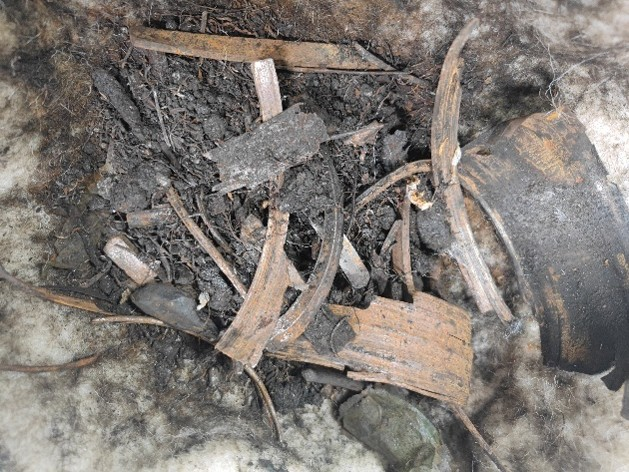
\includegraphics[width=0.5\textwidth]{figure/iron-shavings-sample.jpg}
    \caption{井下封隔器套铣作业中产生的金属碎屑样本}
    \label{fig:iron_shavings_sample}
\end{figure}

\begin{figure}[htbp]
    \centering
    % 子图 (a)
    \subfloat[实际铁屑颗粒]{%
        \begin{minipage}[t]{0.48\linewidth}
            \centering
            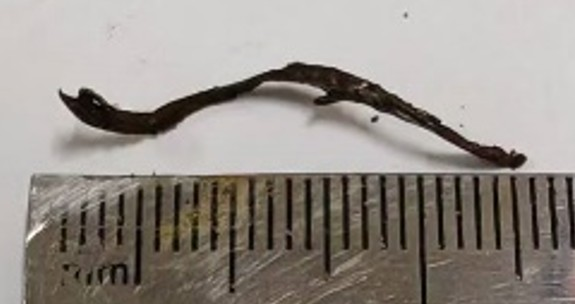
\includegraphics[width=\linewidth]{figure/iron-wire-actual.jpg}
            \label{fig:actual}
        \end{minipage}%
    }
    \hfill
    % 子图 (b)
    \subfloat[铁屑颗粒模型]{%
        \begin{minipage}[t]{0.45\linewidth}
            \centering
            
\includegraphics[width=\linewidth]{figure/iron-wire-model.jpg}
            \label{fig:model}
        \end{minipage}%
    }
    % 总标题
    \caption{铁屑颗粒及仿真模型}
    \label{fig:iron_particle_comparison}
\end{figure}

\begin{table}[htbp]
    \centering
    \caption{铁屑颗粒运移仿真参数}
    \label{tab:simulation_params}
    % 设置列格式：
    % c: 居中
    % p{width}: 固定宽度并自动换行（适合较长的中文名称）
    \begin{tabularx}{.9\textwidth}{cccXc} 
        \toprule % 绘制顶部粗线
        % 表头部分
        序号 & 名称 & 符号 & 数值 & 单位 \\ 
        \midrule % 绘制中间细线
        
        % 数据行
        1 & 水平井筒长度 & $L$ & 1.5 & m \\
        2 & 井筒直径 & $D_H$ & 244.475 & mm \\
        3 & 钻杆直径 & $D_P$ & 88.9 & mm \\
        4 & 颗粒密度 & $\rho_p$ & 7800.0 & kg/m$^3$ \\
        5 & 洗井液密度 & $\rho_l$ & 1000.0、1300.0 & kg/m$^3$ \\
        6 & 井斜角 & $\theta$ & 0.0、45.0、90.0 & $^\circ$ \\
        7 & 洗井液入口流速 & $v_{in}$ & 0.17、0.27 & m/s \\
        8 & 洗井液粘度 & $\mu$ & 1.0、1.7 & mPa$\cdot$s \\
        9 & 沉积域距离井壁高度 & $H$ & 40.0 & mm \\
        10 & 颗粒与井壁静摩擦系数 & $\mu_s$ & 0.15 & - \\
        11 & 颗粒与井壁滑动摩擦系数 & $\mu_k$ & 0.1 & - \\
        
        \bottomrule % 绘制底部粗线
    \end{tabularx}
\end{table}

\subsection{洗井液粘度对铁屑运移规律的影响}
本节选取清水和氯化钠溶液（相对密度为1.3）两种洗井液进行对比。二者均可视为牛顿流体，但粘度不同，对铁屑颗粒的携带效果可能存在差异。在$\theta=90^\circ$、$v_{\mathrm{in}}=0.27\mathrm{m/s}$的条件下，通过仿真对比二者的携屑效果。图\ref{fig:iron_wire_distribution_viscosity}描述的是不同洗井液粘度下井筒内铁屑的分布情况（以颗粒速度着色）。从图中可以看出，洗井液粘度对铁屑颗粒运移效率的影响不大：随着洗井液粘度增大，移动铁屑床的速度略微增大，颗粒运移效率略有提高，出口处的铁屑颗粒有所增多。
%通过对不同洗井液的性能特点进行分析，可以为选择最适合的洗井液粘度提供参考，从而优化洗井操作并提高效率。

\begin{figure}[htbp]
    \centering
    % --- 子图 (a) ---
    % 使用 minipage 控制宽度，这里设为 0.9\textwidth 让图片大一点
    % [t] 表示顶部对齐，防止因为图片高度不同导致错位
    \subfloat[$\mu = 1.0\mathrm{mPa}\cdot\mathrm{s}$]{
        \begin{minipage}[t]{0.8\linewidth}
            \centering
            % 替换为你的第一张图片文件名
            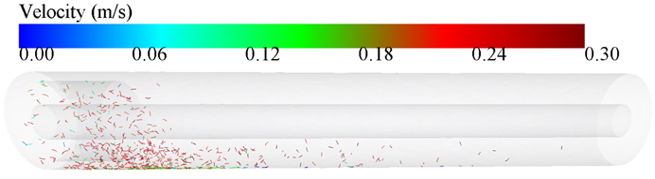
\includegraphics[width=\linewidth]{figure/iron-wire-distribution-1cp-velocity-colored.png} 
            \label{fig:viscosity_1.0}
        \end{minipage}
    }
    \vspace{0pt} % 上下两张图之间的垂直间距，可根据需要调整
    % --- 子图 (b) ---
    \subfloat[$\mu = 1.7\mathrm{mPa}\cdot\mathrm{s}$]{
        \begin{minipage}[t]{0.8\linewidth}
            \centering
            % 替换为你的第二张图片文件名
            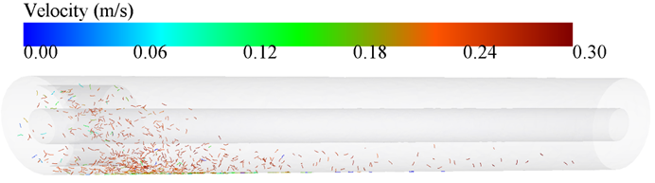
\includegraphics[width=\linewidth]{figure/iron-wire-distribution-1dot7-cp-velocity-colored.png} 
            \label{fig:viscosity_1.7}
        \end{minipage}
    }
    % --- 总标题 ---
    \caption{洗井液粘度对铁屑颗粒速度分布的影响（$\theta=90^\circ$,\ $v_{\mathrm{in}}=0.27\mathrm{m/s}$）}
    \label{fig:iron_wire_distribution_viscosity}
\end{figure}

图\ref{fig:iron_wire_mean_velocity_evolution_viscosity}为两种洗井液粘度下井筒稳态后铁屑颗粒沉积域铁屑颗粒运移速度图。从图中可以看出，$\mu$从$1.0\mathrm{mPa\cdot s}$增加到$1.7\mathrm{mPa\cdot s}$时，粘度增加到$1.7$倍，但铁屑的平均运移速度只增加到$1.04$倍，证明洗井液的粘度对铁屑运移的影响十分有限。
\begin{figure}[htbp]
    \centering
    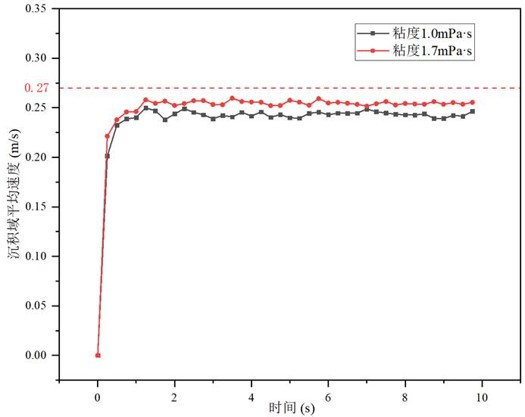
\includegraphics[width=0.7\textwidth]{figure/iron-wire-mean-velocity-evolution-viscosity.jpg}
    \caption{洗井液粘度对铁屑颗粒运移速度时间演变的影响（$\theta=90^\circ$,\ $v_{\mathrm{in}}=0.27\mathrm{m/s}$）}
    \label{fig:iron_wire_mean_velocity_evolution_viscosity}
\end{figure}

\subsection{洗井液流速对铁屑运移规律的影响}

本节探究洗井液流速对井筒环形空间内铁屑颗粒运移的影响。选取了水平段为研究对象，给定$\mu=1.7\mathrm{mPa\cdot s}$。

图\ref{fig:iron_wire_distribution_velocity}描述的是两种流速下井筒内铁屑颗粒分布情况，入口流速对铁屑颗粒运移行为的影响显著。铁屑的密度较大，在两种进口流速下，均表现出在边运移边沉积的现象，在水平管的底部位置有形成颗粒床的趋势。
随着洗井液流速的增加，从颗粒工厂出发的铁屑颗粒整体上产生了更大的轴向位移，颗粒整体的瞬时速度也有增加的趋势。这是由于洗井液流速增大时，铁屑颗粒受到流体沿轴向给予的拖拽力增加，铁屑颗粒沿轴向运移的速度增加。同时，增大的拖拽力也能对抗管壁摩擦效应，颗粒的运移效率增加。
\begin{figure}[htbp]
    \centering
    % --- 子图 (a) ---
    % 使用 minipage 控制宽度，这里设为 0.9\textwidth 让图片大一点
    % [t] 表示顶部对齐，防止因为图片高度不同导致错位
    \subfloat[$v_{\mathrm{in}} = 0.17\mathrm{m/s}$]{
        \begin{minipage}[t]{0.8\linewidth}
            \centering
            % 替换为你的第一张图片文件名
            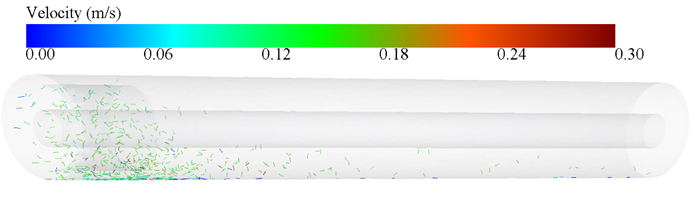
\includegraphics[width=\linewidth]{figure/iron-wire-distribution-1dot7cp-0dot17mpers.png} 
            \label{fig:distribution_velocity_0.17}
        \end{minipage}
    }
    \vspace{0pt} % 上下两张图之间的垂直间距，可根据需要调整
    % --- 子图 (b) ---
    \subfloat[$v_{\mathrm{in}} = 0.27\mathrm{m/s}$]{
        \begin{minipage}[t]{0.8\linewidth}
            \centering
            % 替换为你的第二张图片文件名
            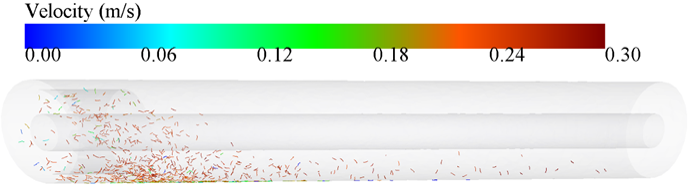
\includegraphics[width=\linewidth]{figure/iron-wire-distribution-1dot7cp-0dot27mpers.png} 
            \label{fig:distribution_velocity_0.27}
        \end{minipage}
    }
    % --- 总标题 ---
    \caption{洗井液流速对铁屑颗粒分布的影响（$\theta=90^\circ$,\ $\mu = 1.7\mathrm{mPa}\cdot\mathrm{s}$）}
    \label{fig:iron_wire_distribution_velocity}
\end{figure}

铁屑颗粒的运动迹线图直观地展现了颗粒的运动轨迹，本文选取了井筒内的部分铁屑颗粒，绘制了两种流速下其迹线图，如图\ref{fig:iron_wire_particle_track_velocity}所示。从图中可以看出，在颗粒工厂中产生的铁屑颗粒一经产生，将很快获得轴向移动速度，这一点可从左上至右下的迹线得到证明；且进口流速越大，迹线的斜率越小，颗粒获得的周向速度也越大。在两种情况下，颗粒落到管底后，以较大幅度弹跳的方式向前运动，而非形成密实的颗粒床以整体的形式运动。在图\ref{fig:distribution_velocity_0.27}中，铁屑颗粒在颗粒工厂右边界附近的迹线混叠密度也低于前者，说明进口流速提升时，颗粒得以弥散开来，颗粒床的形成受到了抑制。

%这两张图的总仿真时间是个很重要的变量。第一个总的仿真时间长，第二个总的仿真时间短。总仿真时间长，颗粒的运动轨迹就会更长，颗粒的运动轨迹就会更密集。总仿真时间短，颗粒的运动轨迹就会更短，颗粒的运动轨迹就会更稀疏。

\begin{figure}[htbp]
	\centering
	% --- 子图 (a) ---
	% 使用 minipage 控制宽度，这里设为 0.9\textwidth 让图片大一点
	% [t] 表示顶部对齐，防止因为图片高度不同导致错位
	\subfloat[$v_{\mathrm{in}} = 0.17\mathrm{m/s}$]{
		\begin{minipage}[t]{0.8\linewidth}
			\centering
			% 替换为你的第一张图片文件名
			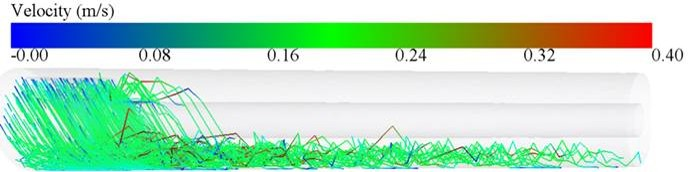
\includegraphics[width=\linewidth]{figure/iron-wire-particle-track-1dot7cp-0dot17mpers.jpg} 
			\label{fig:track_velocity_0.17}
		\end{minipage}
	}
	\vspace{0pt} % 上下两张图之间的垂直间距，可根据需要调整
	% --- 子图 (b) ---
	\subfloat[$v_{\mathrm{in}} = 0.27\mathrm{m/s}$]{
		\begin{minipage}[t]{0.8\linewidth}
			\centering
			% 替换为你的第二张图片文件名
			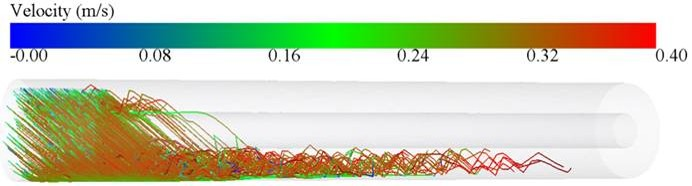
\includegraphics[width=\linewidth]{figure/iron-wire-particle-track-1dot7cp-0dot27mpers.jpg} 
			\label{fig:track_velocity_0.27}
		\end{minipage}
	}
	% --- 总标题 ---
	\caption{洗井液流速对铁屑颗粒分布的影响（$\theta=90^\circ$,\ $\mu = 1.7\mathrm{mPa}\cdot\mathrm{s}$）}
	\label{fig:iron_wire_particle_track_velocity}
\end{figure}

图\ref{fig:iron_wire_mean_velocity_evolution_incoming_velocity}给出了$v_{\mathrm{in}}=0.17\mathrm{m/s}$,\ $0.27\mathrm{m/s}$两种情况下铁屑颗粒在沉积域中运移速度定量结果。洗井液流动产生的携屑作用足以克服井筒内壁摩擦作用，沉积在井筒底部的铁屑形成移动铁屑床。颗粒的平均轴向运动速度是小于来流（平均）速度，这说明铁屑颗粒在井筒内的运移过程中，受到井壁摩擦力的影响。随着时间的推移，铁屑颗粒在沉积域中的平均运移速度逐渐趋于稳定，表明颗粒在井筒内的运移达到了动态平衡状态。随着洗井液流速的增加，井筒内沉积域铁屑颗粒运移速度也会大幅度增加，于是，洗井液的流速对铁屑运移有显著影响。
\begin{figure}[htbp]
	\centering
	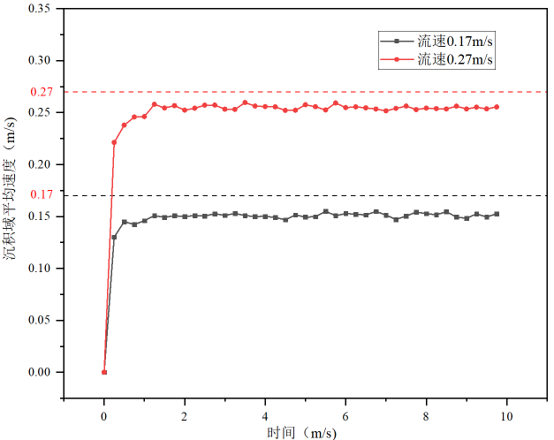
\includegraphics[width=0.7\textwidth]{figure/iron-wire-mean-velocity-evolution-incoming-velocity.png}
	\caption{洗井液速度对铁屑颗粒运移速度时间演变的影响（$\mu=1.7\mathrm{mPa\cdot s}$）}
	\label{fig:iron_wire_mean_velocity_evolution_incoming_velocity}
\end{figure}

\subsection{井斜对铁屑运移规律的影响}
本节将探究井斜对于井筒环形空间内铁屑颗粒运移的影响。选取了直井（$\theta = 0^\circ$）、45°斜井（$\theta = 45^\circ$）和水平井（$\theta = 90^\circ$）三种井斜，洗井液入口流速为$v_\mathrm{in}=0.27\mathrm{m/s}$，粘度取$\mu=1.7\mathrm{mPa\cdot s}$。

图\ref{fig:iron_wire_distribution_3angles}描述了不同井斜角度下井筒内铁屑颗粒瞬时分布情况。从图中可以看出，直井（$\theta = 0^\circ$）中井筒中铁屑不能向上迁移，目前的流体拖曳力不足以克服重力的作用。$\theta = 45^\circ$斜井中，铁屑床主要沉积在颗粒工厂附近的底部井壁上，距流体入口较近，流体出口附近几乎没有铁屑颗粒。$\theta = 90^\circ$的水平井，颗粒同样会聚集在井壁上，但颗粒床迁移的距离更远，聚集度更低，且出口处颗粒的数量比$\theta = 45^\circ$斜井中更多。
%$\theta = 45^\circ$和$\theta = 90^\circ$两种情况下，铁屑床都由移动床和静止床两部分组成，静止床的出现意味着上部铁屑积压，流体拖曳力、重力和摩擦作用相平衡；移动床的出现意味着流体的拖拽作用足以克服重力和管壁摩擦对单个铁屑颗粒的作用，使铁屑持续运移。表明，单个颗粒的行为有别于一群颗粒的行为，颗粒-颗粒之间的相互作用会影响颗粒的运移行为。
结合三种情况可以推测：第一，在直井中，作业产生的铁屑一定会下落至井底；第二，存在一个临界井斜$\theta_c$，当$\theta < \theta_c$时，铁屑颗粒会一直下落至井底形成堆积，而当$\theta > \theta_c$时，铁屑颗粒会在井筒壁面中形成堆积；第三，$\theta_c<45^\circ$，且其大小与流体的流速、粘度以及铁屑颗粒的密度、形状等因素相关。

\begin{figure}[htbp]
	\centering
	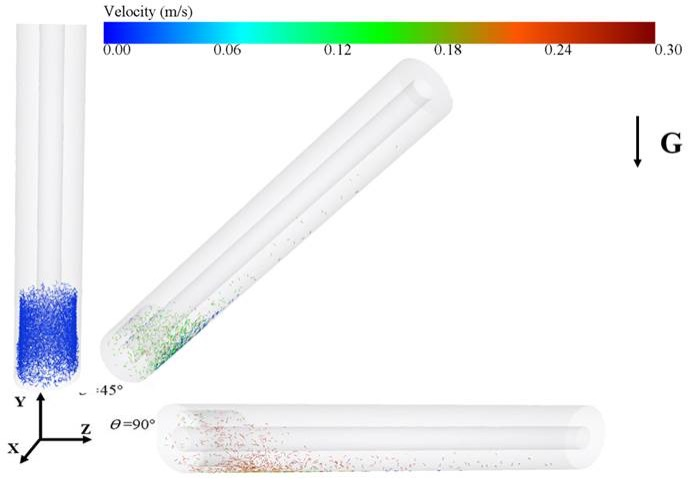
\includegraphics[width=0.7\textwidth]{figure/iron-wire-distribution-1dot7cp-0dot27mpers-3angles.jpg}
	\caption{井斜角对铁屑颗粒分布情况}
	\label{fig:iron_wire_distribution_3angles}
\end{figure}

铁屑颗粒的流动迹线图可以直观地描述颗粒的运动轨迹。首先选取井筒内的部分铁屑颗粒，绘制不同井斜角度下部分铁屑流动迹线图，如图\ref{fig:iron_wire_track_3angles}所示。直井（$0^\circ$）中铁屑运动轨迹平直，说明铁屑几乎不与井壁产生接触（或碰撞），短促的轨迹说明颗粒将向井底沉积，不能持续随流运移。各井斜条件下井壁处与颗粒工厂处的颗粒速度均较小，水平井环空内的颗粒速度大于斜井。这是由于井筒轴线与重力方向的夹角增大，环空中颗粒所受重力的影响愈发显著，颗粒在自身重力作用下下沉加快，洗井液在轴向上不足以提供足够的悬浮能量，颗粒堆积到底部后形成颗粒床，运移效率明显降低。

\begin{figure}[htbp]
	\centering
	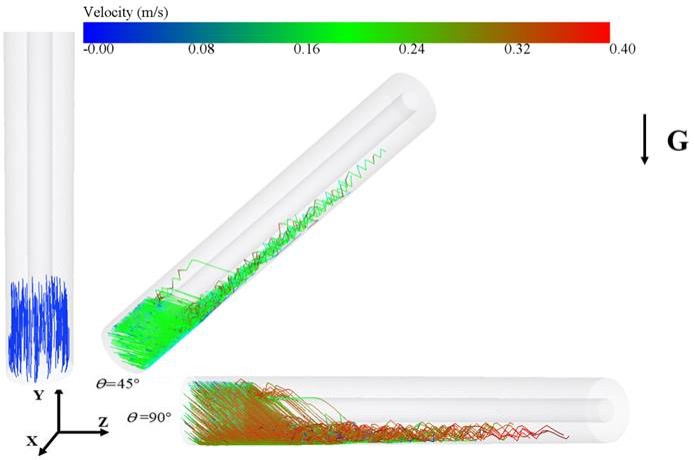
\includegraphics[width=0.7\textwidth]{figure/iron-wire-particle-track-1dot7cp-0dot27mpers-3angles.jpg}
	\caption{井斜角对铁屑运动轨迹的影响}
	\label{fig:iron_wire_track_3angles}
\end{figure}

斜井（$\theta = 45^\circ$）中移动铁屑床的平均运移速度小于水平井（$\theta = 90^\circ$），如图\ref{fig:iron_wire_velocity_3angles}所示。水平井中铁屑颗粒的运移速度接近环空平均流速，而斜井中铁屑颗粒的运移速度仅为环空平均流速的一半左右。

\begin{figure}[htbp]
	\centering
	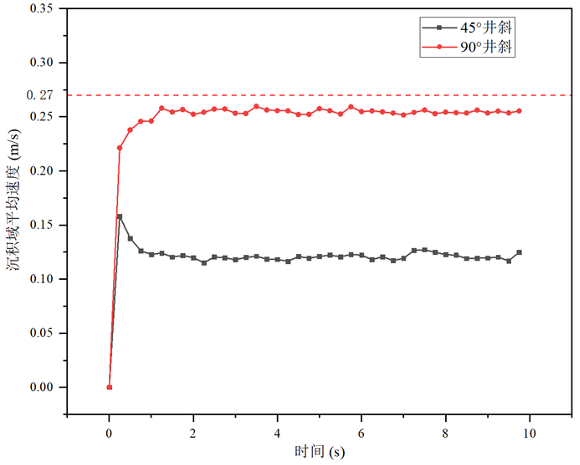
\includegraphics[width=0.7\textwidth]{figure/iron-wire-mean-velocity-evolution-3angles.png}
	\caption{井斜角对铁屑运动速度的影响}
	\label{fig:iron_wire_velocity_3angles}
\end{figure}

综合上述仿真结果可以发现，洗井液粘度增大和环空流速提高对铁屑颗粒的运移效率均有正向作用，因此选用更高粘度的洗井液、采用更大的洗井排量有助于铁屑颗粒从井筒中排出。但是，铁屑的运移行为受井筒倾角影响很大：在直井和小斜度井中，铁屑难以通过常规的洗井液循环方式排出，需开发具有\textbf{吸附}、\textbf{过滤}功能的\textbf{专用清洁工具}将铁屑从井筒中捞出。针对丝状铁屑的仿真结果可进一步推广至片状、块状铁屑等情形，此类高密度碎屑在井筒中的运移能力较差。

\section{井筒内结垢物运移及分布规律研究}
海上油井钡锶垢是由地层水与注入水（如海水）混合后，因钡（$\mathrm{Ba^{2+}}$）、锶（$\mathrm{Sr^{2+}}$）离子与硫酸根（$\mathrm{SO_4^{2-}}$）或碳酸根（$\mathrm{CO_3^{2-}}$）结合形成的难溶性无机盐（如硫酸钡、硫酸锶），在井筒、管道或设备表面沉积形成的坚硬垢层；其生成受高温高压、高矿化度及流动条件影响，易堵塞油流通道、加剧设备腐蚀，甚至因伴生放射性物质（如镭）带来安全与环保风险。
研究钡锶垢的运移规律在油井洗井中至关重要，通过明确垢颗粒的迁移和沉降特性，优化洗井工艺参数，高效清除井筒和近井地带的顽固垢层，避免二次堵塞或地层伤害，从而恢复油井产能并延长寿命；同时可预测垢的沉积风险，指导防垢措施以减少设备腐蚀和放射性污染，降低维护成本与环境危害，并为建立结垢动力学模型、开发新型洗井技术提供理论支撑，最终实现安全、经济、环保的油田开发目标。

建立两种尺寸不同的钡锶垢颗粒模型，如图\ref{fig:BaSr_particle}所示。通过调研钡锶垢的物理性质及性状，将其运移仿真参数列于表\ref{tab:basr_simulation_params}。

\begin{figure}[htbp]
    \centering
    % 子图 (a)
    \subfloat[钡锶垢实物]{%
        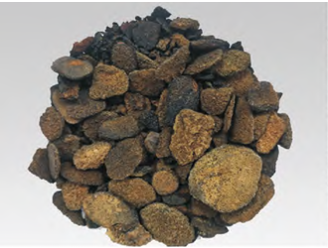
\includegraphics[width=0.48\linewidth]{figure/BaSr-sample.png}%
        \label{fig:BaSr_sample}%
    }
    \hfill
    % 子图 (b)
    \subfloat[SEM微观形貌]{%
        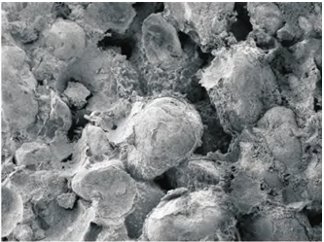
\includegraphics[width=0.48\linewidth]{figure/BaSr-SEM.png}%
        \label{fig:BaSr_SEM}%
    }
    \vspace{1em}
    % 子图 (c)
    \subfloat[垢仿真模型示意图]{%
        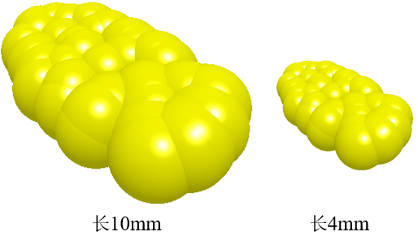
\includegraphics[width=0.5\linewidth]{figure/BaSr-model.png}%
        \label{fig:BaSr_model}%
    }
    \caption{钡锶垢颗粒及仿真模型对比}
    \label{fig:BaSr_particle}
\end{figure}

\begin{table}[htbp]
    \centering
    \caption{锁锶垢颗粒运移仿真参数}
    \label{tab:simulation_params}
    \begin{tabularx}{.9\textwidth}{cCCc}
        \toprule % 顶部粗线
        名称 & 符号 & 数值 & 单位 \\
        \midrule % 中间细线
        水平井筒长度 & $L$ & 1.5 & m \\
        井筒直径 & $D_H$ & 177.8 & mm \\
        钻杆直径 & $D_P$ & 88.9 & mm \\
        颗粒密度 & $\rho_P$ & 4336.0 & kg/m$^3$ \\
        洗井液密度 & $\rho_l$ & 1300.0 & kg/m$^3$ \\
        井斜角度 & $\theta$ & 0、45、90 & $^\circ$ \\
        洗井液入口流速 & $v_{in}$ & 0.37、0.59 & m/s \\
        洗井液粘度 & $\mu$ & 1.7 & mPa$\cdot$s \\
        沉积域距离井壁高度 & $H$ & 20.0 & mm \\
        颗粒与井壁静摩擦系数 & $\mu_s$ & 0.5 & - \\
        颗粒与井壁滑动摩擦系数 & $\mu_k$ & 0.4 & - \\
        \bottomrule % 底部粗线
    \end{tabularx}
\end{table}

\subsection{洗井液流速对钡锶垢运移规律的影响}

选取井斜$\theta = 45^\circ$，洗井液入口流速$V_{\mathrm{in}}$取$0.37\mathrm{m/s}$和$0.59\mathrm{m/s}$两种，洗井液粘度取$1.7\mathrm{mPa\cdot s}$，钡锶垢颗粒有两种尺寸，特征长度约为$10\mathrm{mm}$和$4\mathrm{mm}$。

图\ref{fig:Ba_Sr_distribution}描述的是不同洗井液流速下井筒内钡锶垢颗粒的分布情况，入口流速对钡锶垢颗粒运移效率的影响十分明显。随着洗井液流速增大，钡锶垢颗粒的运移速度逐渐增大。由于洗井液入口流速增大，产生于颗粒工厂的钡锶垢颗粒及悬浮层颗粒具有更大的轴向位移，在相同的仿真时间内，流速高时井筒内钡锶垢颗粒距离流体入口更远。
\begin{figure}[htbp]
	\centering
	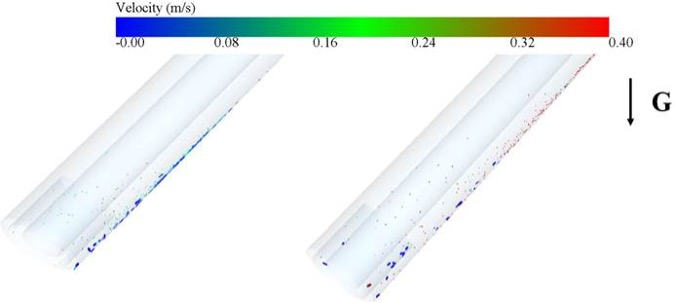
\includegraphics[width=0.7\textwidth]{figure/BaSr-distribution-Vin.jpg}
	\caption{钡锶垢颗粒在井筒中的运移}
	\label{fig:Ba_Sr_distribution}
\end{figure}

图\ref{fig:Ba_Sr_velocity_size}为钡锶垢在井筒洗井液流速$V_{\mathrm{in}}=0.37\mathrm{m/s}$和$V_{\mathrm{in}}=0.59\mathrm{m/s}$稳态后颗粒沉积域运移速度图。选取Z方向为竖直向上方向。$V_{\mathrm{in}}=0.37\mathrm{m/s}$时，大垢落到井壁上后会滑向井底，小垢在进入沉积域后会以远远低于井筒内流体的速度(约为$0.05\mathrm{m/s}$)缓慢向压力出口运移。$V_{\mathrm{in}}=0.59\mathrm{m/s}$时，大垢在进入沉积域之后Z方向速度几乎为零，少许的速度波动是由颗粒碰撞引起的，因此大垢在接触井壁后会在井壁上发生沉积现象，小垢在进入沉积域后会以低于井筒内流体的速度向压力出口运移，运移速度为$0.25\mathrm{m/s}$左右。

\begin{figure}[htbp]
	\centering
	\subfloat[$V_{\mathrm{in}}=0.37\mathrm{m/s}$]{%
	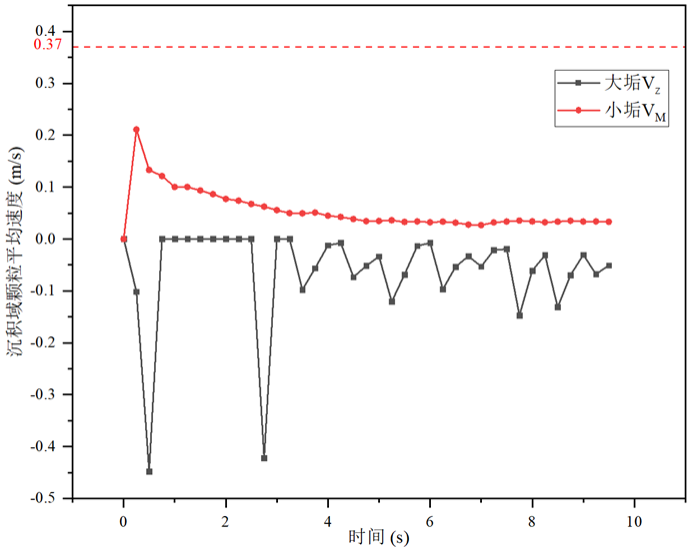
\includegraphics[width=0.48\textwidth]{figure/BaSr-mean-velocity-evolution-vin-dot37.png}
	}
	\subfloat[$V_{\mathrm{in}}=0.59\mathrm{m/s}$]{%
	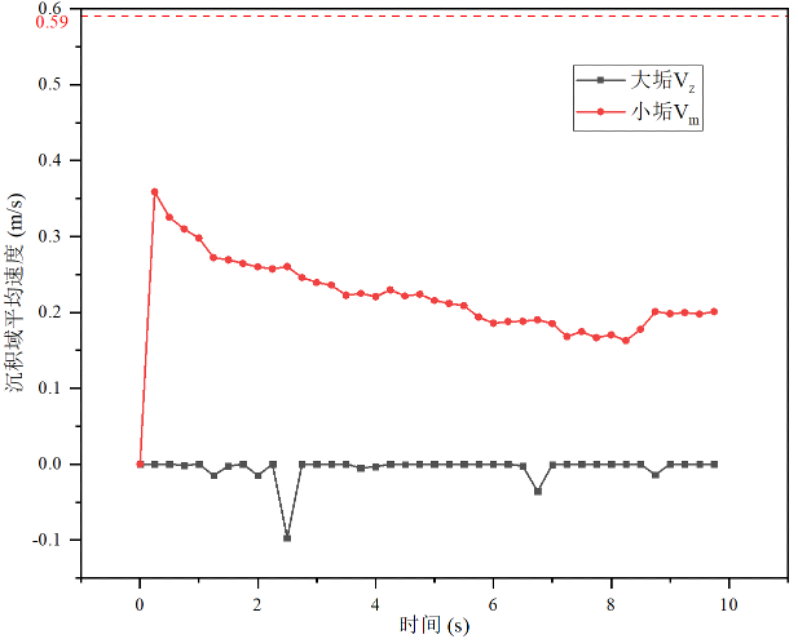
\includegraphics[width=0.48\textwidth]{figure/BaSr-mean-velocity-evolution-vin-dot59.png}
	}
	\caption{钡锶垢颗粒在沉积域运移平均速度演化}
	\label{fig:Ba_Sr_velocity_size}
\end{figure}

\subsection{井斜对钡锶垢运移规律的影响}

图\ref{fig:Ba_Sr_distribution_3angles}描述了井斜角变化时井筒内钡锶垢颗粒分布情况。$\theta=45^\circ$与$\theta=90^\circ$井斜下的钡锶垢颗粒都沉积在井底并以一定的速度向压力出口方向运移，其中$\theta=45^\circ$井筒内钡锶垢颗粒运移速度要大于$\theta=90^\circ$井筒内钡锶垢的运移速度，大颗粒钡锶垢在$\theta=45^\circ$与$\theta=90^\circ$井筒环空中均能够观察到，在直井（$\theta=0^\circ$）井筒环空中没有发现大颗粒钡锶垢，推测由于重力作用大颗粒钡锶垢产生后即下落至井底。而小颗粒钡锶垢运移速度随着井筒倾角的增大而减小，可见井筒倾角对钡锶垢运移效率有很大影响，其影响要以颗粒实际大小为准。

\begin{figure}[htbp]
	\centering
	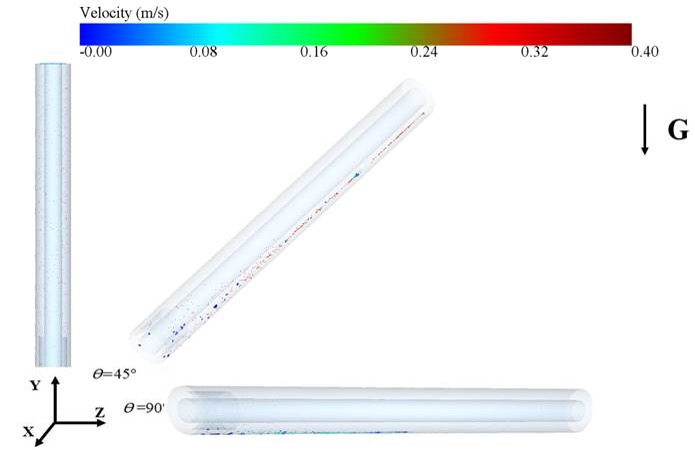
\includegraphics[width=0.7\textwidth]{figure/BaSr-distribution-3angles.jpg}
	\caption{钡锶垢颗粒在井筒中的运移}
\label{fig:Ba_Sr_distribution_3angles}
\end{figure}


图\ref{fig:Ba_Sr_velocity_3angles}(a)描述的是不同井斜下大颗粒钡锶垢井筒内运移速度变化，从图中可以看出，井斜45°与井斜90°情况下大颗粒钡锶垢因为重力影响在接触井壁后运移速度几乎为零，因此会在井壁产生沉积现场。井斜0°情况下大颗粒钡锶垢在井筒环空中运移，速度小于零说明大颗粒钡锶垢在以流体速度相反的方向运移，预测会在井底产生沉积。图\ref{fig:Ba_Sr_velocity_3angles}(b)描述的是不同井斜下小颗粒钡锶垢井筒内运移速度变化，从图中可以看出，随着井斜角的增加，钡锶垢在井筒内的运移速度逐渐减小。0°井斜下，钡锶垢在四秒左右即有颗粒到达压力出口，因为到达压力出口的钡锶垢颗粒速度减为0，随着越来越多的钡锶垢颗粒到达压力出口，其平均运移速度逐渐减小。45°与90°井斜下，钡锶垢颗粒由于重力作用在接触井筒内壁后会以一定速度向压力出口运移。由此可见，井斜可以明显影响钡锶垢颗粒的运移效率。

\begin{figure}[htbp]
	\centering
	\subfloat[$V_{\mathrm{in}}=0.37\mathrm{m/s}$]{%
	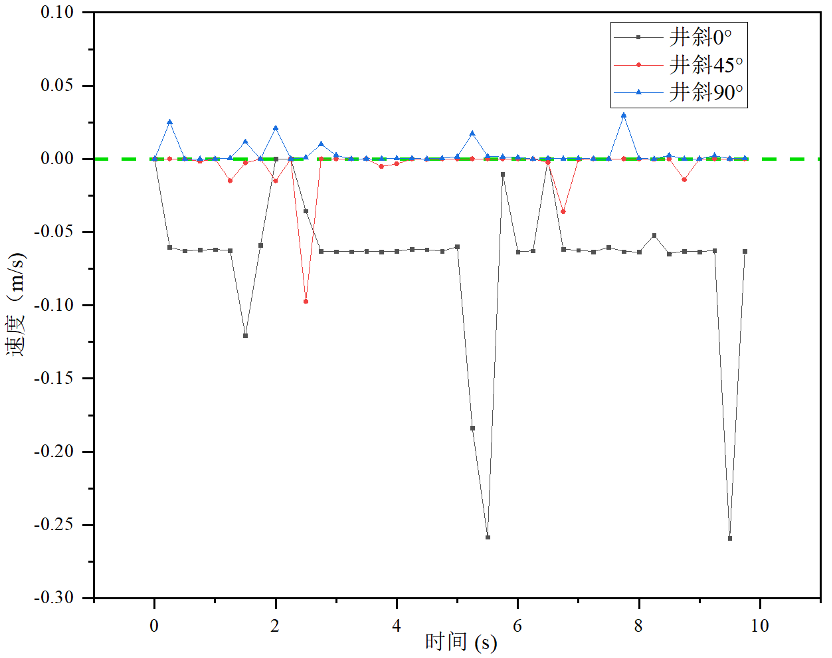
\includegraphics[width=0.48\textwidth]{figure/BaSr-mean-velocity-evolution-big-size.png}
	}
	\subfloat[$V_{\mathrm{in}}=0.59\mathrm{m/s}$]{%
	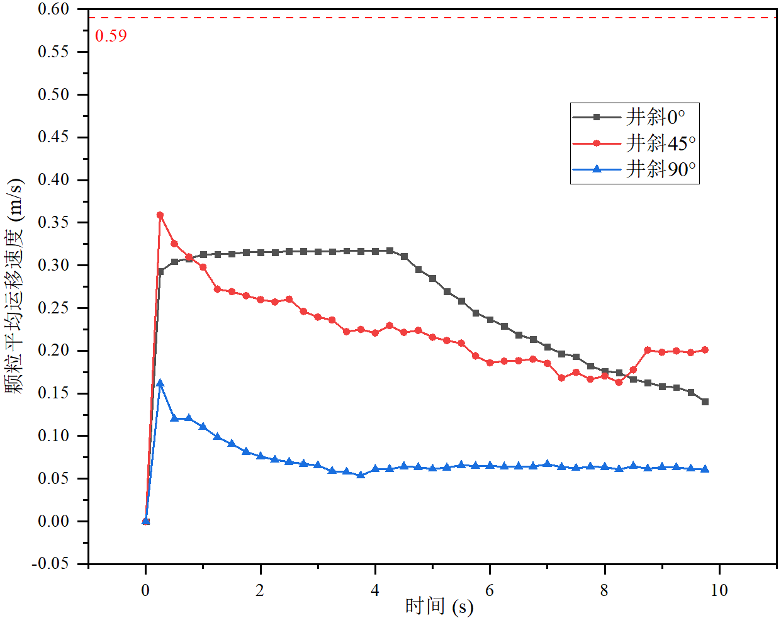
\includegraphics[width=0.48\textwidth]{figure/BaSr-mean-velocity-evolution-small-size.png}
	}
	\caption{钡锶垢颗粒在沉积域运移平均速度演化}
	\label{fig:Ba_Sr_velocity_3angles}
\end{figure}

仿真结果表明，洗井液流速增大时小钡锶垢颗粒的运移速度相应增大，因此在洗井作业中可适当提高洗井液流速以提升洗井效率。在流速0.59m/s的情况下，三种井斜工况下大钡锶垢颗粒均会发生沉积：0°井斜时沉积在井底，45°井斜时先沉积在井壁、随后向井底滑移，90°井斜时沉积在井壁，因此冲洗大块钡锶垢需要更高的泵送排量。在45°与90°井斜下，大小钡锶垢都会发生沉积，且小钡锶垢的运移速度远小于环空流体流速，因此在作业时应重点清洗斜井段与水平井段。

\section{井筒内蜡垢运移及分布规律研究}

油井中的蜡垢是原油中高碳链石蜡（$C_{18}$～$C_{60}$烃类）在开采过程中因温度、压力等条件变化析出并沉积形成的固态或半固态混合物，主要成分为石蜡、沥青质、胶质及机械杂质。其形成机制与原油组成和开采环境密切相关：当原油从高温高压地层流向井筒时，随着温度降低和压力释放，石蜡溶解度下降，逐步结晶析出并附着在管壁、泵阀等设备表面，形成致密垢层。蜡垢的危害显著：会堵塞油管导致产量下降，增加抽油能耗，加速设备磨损，甚至引发卡泵事故。
研究蜡垢运移规律对油井洗井过程至关重要，通过揭示蜡垢运移与沉积的动态机制，能够优化洗井参数，提升清蜡效率并降低井筒堵塞风险；在保障油井稳产、提高经济效益的同时，减少环境污染，推动油气开采的绿色高效发展。本节对蜡垢进行迁移仿真所用到的仿真条件如表\ref{tab:wax_params}所示。

\begin{table}[htbp]
    \centering
    \caption{蜡垢运移仿真参数}
    \label{tab:wax_params}
    \begin{tabularx}{.9\textwidth}{CCCC}
        \toprule % 顶部粗线
        名称 & 符号 & 数值 & 单位 \\
        \midrule % 中间细线
        水平井筒长度 & $L$ & 1.5 & m \\
        井筒直径 & $D_H$ & 177.8 & mm \\
        钻杆直径 & $D_P$ & 88.9 & mm \\
        颗粒密度 & $\rho_P$ & 800.0 & kg/m$^3$ \\
        洗井液密度 & $\rho_l$ & 1300.0 & kg/m$^3$ \\
        井斜角度 & $\theta$ & 0、45、90 & $^\circ$ \\
        洗井液入口流速 & $v_{in}$ & 0.37、0.59 & m/s \\
        洗井液粘度 & $\mu$ & 1.7 & mPa$\cdot$s \\
        沉积域距离井壁高度 & $H$ & 20 & mm \\
        颗粒模型大小 & - & 1、2、3、4 & mm \\
        颗粒与井壁静摩擦系数 & $\mu_s$ & 0.6 & - \\
        颗粒与井壁滑动摩擦系数 & $\mu_k$ & 0.2 & - \\
        \bottomrule % 底部粗线
    \end{tabularx}
\end{table}

\subsection{洗井液流速对蜡垢运移规律的影响}

本节改变洗井液流速，探究其对井筒环形空间内蜡垢颗粒运移的影响。取井斜45°，洗井液入口流速分别为0.37m/s、0.59m/s，粘度取$1.7\mathrm{mPa\cdot s}$，蜡垢颗粒粒径取2mm、4mm、6mm、8mm四种。

图1.41(a)描述了流体流速0.37m/s不同粒径下45°井筒内沉积域蜡垢颗粒平均速度情况，从图中可以看出，进入沉积域后蜡垢会以大于井筒内流体的速度向压力出口运移，随着粒径的增大，其运移速度也越来越大，并在四秒后蜡垢颗粒陆续到达压力出口。图1.41(b)描述了环空流体流速0.59m/s不同粒径下45°井筒内沉积域蜡垢颗粒平均速度情况，从图中可以看出，随着环空流体流速增大，蜡垢颗粒的运移速度也会增大，环空流体流速0.59m/s条件下，蜡垢颗粒在2.5秒后到达压力出口，相对于环空流体流速0.37m/s条件，蜡垢颗粒到达压力出口的速度变快。由此可见，环空流体流速对于蜡垢颗粒运移效率的影响显著。
\begin{figure}[htbp]
	\centering
	\subfloat[$V_{\mathrm{in}}=0.37\mathrm{m/s}$]{%
	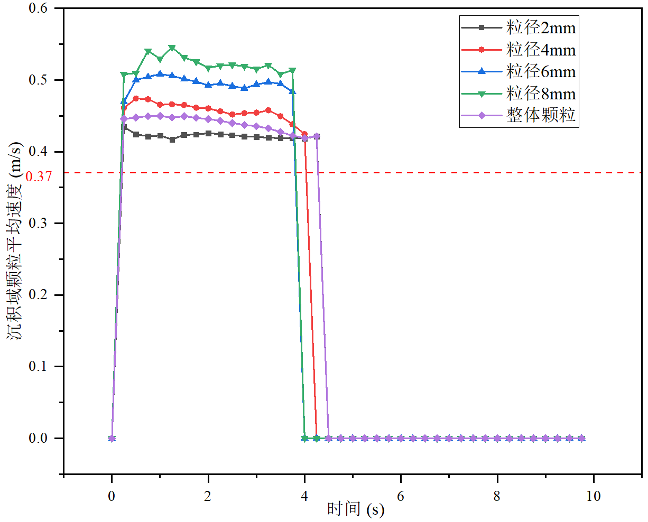
\includegraphics[width=0.48\textwidth]{figure/Wax-mean-velocity-Vin-dot37mpersec.png}
	}
	\subfloat[$V_{\mathrm{in}}=0.59\mathrm{m/s}$]{%
	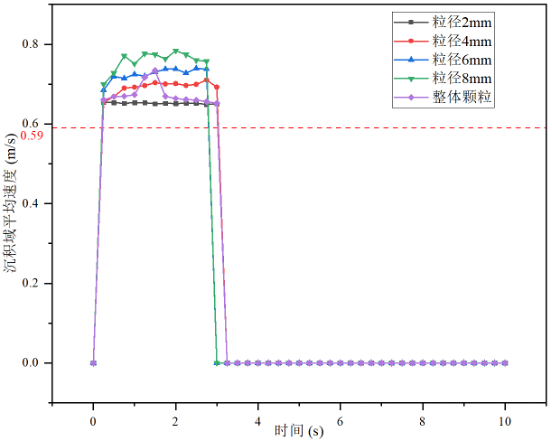
\includegraphics[width=0.48\textwidth]{figure/Wax-mean-velocity-Vin-dot59mpersec.png}
	}
	\caption{蜡垢颗粒在沉积域运移平均速度演化}
	\label{fig:Wax_velocity_particle_size}
\end{figure}

\subsection{井斜对蜡垢颗粒运移规律的影响}
本节改变井筒倾角，探究其对井筒环形空间内蜡垢颗粒运移的影响。选取井斜$\theta_c = 0^\circ$、45°、90°，洗井液入口流速为0.59m/s，粘度取$1.7\mathrm{mPa\cdot s}$，蜡垢颗粒粒径取2mm、4mm、6mm、8mm四种。图\ref{fig:wax_velocity_3angles}(a)描述了环空流体流速0.59m/s时0°井筒内不同粒径蜡垢颗粒在沉积域的平均速度变化情况：随着蜡垢颗粒粒径增大，其运移速度也增大，且均高于环空流体流速；在环空流体流速0.59m/s条件下，蜡垢颗粒在2.5s后到达压力出口。与45°井筒倾角工况相比，0°倾角井筒内蜡垢颗粒的最大运移速度更高，但其达到最大运移速度的时间长于45°井筒倾角工况。图\ref{fig:wax_velocity_3angles}(b)描述了环空流体流速0.59m/s时90°井筒内不同粒径蜡垢颗粒在沉积域的平均速度变化情况：随着蜡垢颗粒粒径增大，其运移速度反而减小，且均低于环空流体流速，可见摩擦力作用会导致蜡垢颗粒的运移速度下降；在环空流体流速0.59m/s条件下，蜡垢颗粒在4s后到达压力出口。与0°、45°井筒倾角工况相比，90°倾角井筒内蜡垢颗粒的最大运移速度明显下降，到达压力出口的时间变长，运移效率降低。


\begin{figure}[htbp]
	\centering
	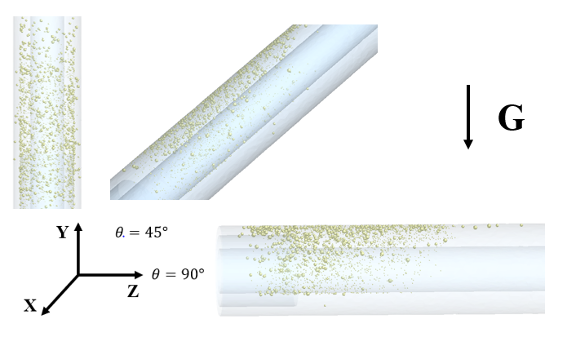
\includegraphics[width=0.7\textwidth]{figure/wax-distribution-3angles.png}
	\caption{不同井斜下蜡垢颗粒井筒内运移分布图}
\label{fig:wax_distribution_3angles}
\end{figure}


\begin{figure}[htbp]
	\centering
	\subfloat[$\theta=0^\circ$]{%
	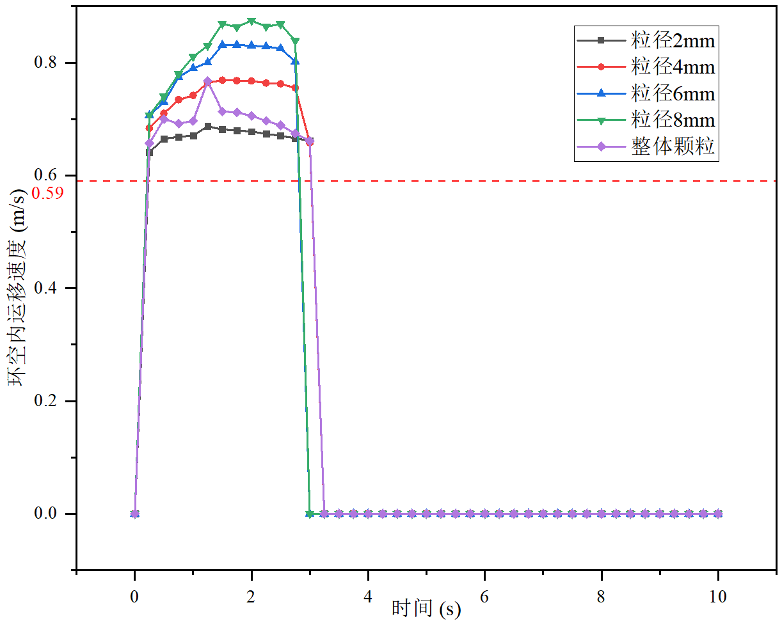
\includegraphics[width=0.48\textwidth]{figure/Wax-mean-velocity-Vin-dot59mpersec-theta-0.png}
	}
	\subfloat[$\theta=90^\circ$]{%
	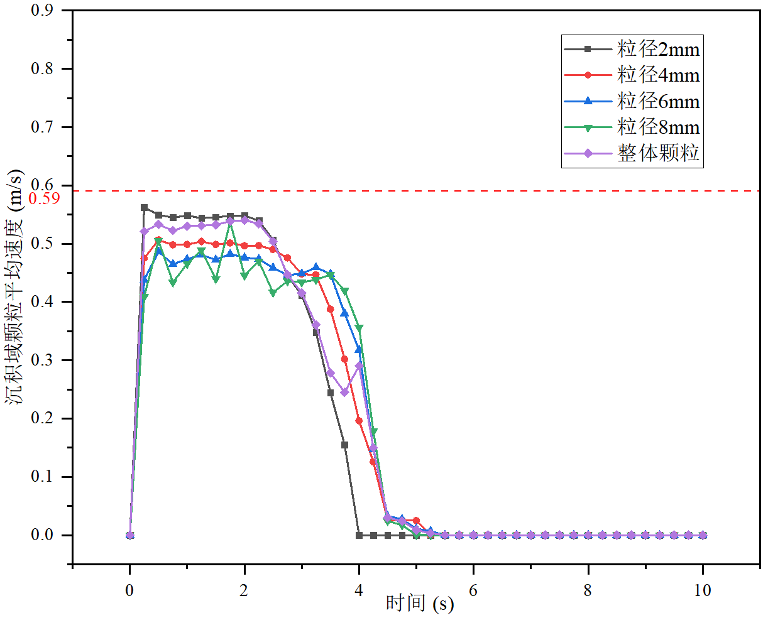
\includegraphics[width=0.48\textwidth]{figure/Wax-mean-velocity-Vin-dot59mpersec-theta-90.png}
	}
	\caption{井斜对蜡垢颗粒在沉积域运移平均速度演化的影响}
	\label{fig:wax_velocity_3angles}
\end{figure}

通过这些仿真发现，蜡垢颗粒的运移规律跟颗粒大小有关，在0°与45°井斜条件下，蜡垢颗粒的粒径越大，其运移速度越大。90°井斜条件下，蜡垢颗粒越小，其运移速度越大。随着井斜角度增加，蜡垢颗粒的运移速度也逐渐减小。 在各个井段并未发生蜡垢沉积现象。

\section{本章小结}

本章针对修井及洗井作业中砂砾、铁屑、结垢物（钡锶垢）和蜡质四类典型颗粒物在井筒内的运移及分布问题，基于流体动力学与颗粒动力学理论，建立了 EDEM--Fluent 双向耦合的液固两相流数值模拟方法，并以洗井液流速 $v_{\mathrm{in}}$、粘度 $\mu$ 和井斜角 $\theta$ 为核心控制变量，系统研究了四类颗粒在井筒环空内的运移轨迹、沉积速率及空间分布特征，主要结论如下：

（1）建立了井筒环空颗粒运移的 EDEM--Fluent 耦合仿真方法。颗粒相采用 Hertz--Mindlin 接触模型描述颗粒间以及颗粒与壁面间的接触、碰撞与摩擦作用，对含湿、存在液桥力的工况可采用 Hertz--Mindlin with JKR 接触模型；液固相间作用采用 Gidaspow 曳力模型，并计入 Saffman 剪切升力与 Magnus 旋转升力；液相采用 N--S 方程与标准 $k-\epsilon$ 湍流模型求解（部分工况采用 $SST\ k-\omega$ 模型），通过耦合接口实现颗粒运动与流场动量的双向传递。计算模型取长 $1.5$ m 的环空管段，模拟 $\phi 88.9$ mm 钻杆与 $\phi 244.475$ mm（$9$-5/8\inch）、$\phi 177.8$ mm（$7$\inch）井筒的组合工况，井斜角取 $0^\circ$、$45^\circ$、$90^\circ$，洗井液流速取 $0.17\sim0.69$ m/s，粘度取 $1.0\sim5.0\ \mathrm{mPa}\cdot\mathrm{s}$。

（2）基于现场砂样粒度分级统计结果（中砂 35.29\%、细砂 47.15\%、极细砂 13.99\%）建立了 9.9 万个不同粒径砂砾颗粒的仿真模型，获得了环空内砂砾的沉降与分布规律。钻杆静止时环空内砂砾质量在约 30 s 后趋于稳定，稳定沉积量平均约 $63.294$ kg；由于环空上部为流体高速区、下部为低速区，砂砾受重力作用大量沉降于环空下部低速区并形成砂床，砂砾床主要沉积在水平段，井斜角增大后井斜段内砂砾体积分数明显减小。随洗井液流速由 $0.17$ m/s 增至 $0.69$ m/s，砂床最高点（b 点）高度由 $68$ mm 降至 $32$ mm，且砂砾体积分数减小、砂砾流速增大，表明增大排量可增强流体携砂能力、降低砂堵风险；随洗井液粘度由 $1.0\ \mathrm{mPa}\cdot\mathrm{s}$ 增至 $5.0\ \mathrm{mPa}\cdot\mathrm{s}$，砂床最高点高度由 $77.5$ mm 降至 $25$ mm，但砂砾流速呈减小趋势，即增大粘度在提高携砂能力的同时会降低环空流体的流动性、延长砂砾上返时间。因此，工程上减小砂堵风险应以增大冲砂排量为主要手段，以适度提高洗井液粘度为辅。

（3）明确了颗粒在工具与井筒环空内沉积的“危险位置”。以外部功能单元最多、结构最复杂的“四合一”工具扶正器与强磁部位和 $7$\inch 井筒构成的环空为对象，在环空流速 $0.37$、$0.59$ m/s 下开展仿真，结果表明部分砂砾会因重力作用在工具前端产生堆积，并在强磁部件的凹槽内少量滞留；环空流速增大后颗粒的轴向位移与运移效率明显提高。工具的导流结构可引导砂砾随流运移，与增大冲砂排量相配合能够有效降低砂堵概率，为工具安全作业提供保障。

（4）揭示了铁屑颗粒“粘度弱敏感、流速强敏感、井斜角决定性”的运移规律。以井下封隔器套铣作业返出碎屑中的丝状铁屑（密度 $7800$ kg/m$^{3}$）为典型建模对象：颗粒在沉积域中的平均轴向速度始终小于来流平均速度，表明井壁摩擦对颗粒运移具有显著阻滞作用，随时间推移运移速度逐渐趋于稳定，颗粒运移达到动态平衡状态；粘度由 $1.0\ \mathrm{mPa}\cdot\mathrm{s}$ 增至 $1.7\ \mathrm{mPa}\cdot\mathrm{s}$（增至 $1.7$ 倍）时，沉积域内颗粒的平均运移速度仅增至 $1.04$ 倍，说明洗井液粘度对铁屑运移的影响十分有限；流速由 $0.17$ m/s 增至 $0.27$ m/s 时，颗粒的轴向位移与瞬时速度大幅提高，颗粒床的形成受到抑制，说明流速是铁屑运移最敏感的控制因素；井斜角的影响最为显著，直井（$\theta=0^\circ$）中流体拖曳力不足以克服重力，铁屑不能上返、必然下落至井底；$45^\circ$ 斜井中铁屑床堆积在靠近颗粒工厂一侧的底部井壁，出口附近几乎没有颗粒；水平井（$\theta=90^\circ$）中颗粒床迁移距离更远、聚集度更低、出口处颗粒数量更多，但移动铁屑床的平均运移速度仅约为环空平均流速的一半。据此推测存在临界井斜角 $\theta_c<45^\circ$：当 $\theta<\theta_c$ 时铁屑一致下落至井底形成堆积，当 $\theta>\theta_c$ 时铁屑在井壁堆积。上述结论可推广至片状、块状等高密度金属屑。可见在直井与小斜度井中，铁屑难以通过常规洗井液循环排出井筒，必须依靠具备\textbf{吸附}、\textbf{过滤}功能的\textbf{专用清洁工具}。

（5）阐明了结垢物（钡锶垢）颗粒的运移与沉积特征。以密度 $4336$ kg/m$^{3}$、特征长度分别约为 $10$ mm 和 $4$ mm 的两种钡锶垢颗粒为对象：随洗井液流速由 $0.37$ m/s 增至 $0.59$ m/s，垢颗粒的运移速度与轴向位移均增大；但在 $0.59$ m/s 时，三种井斜工况下的大颗粒垢均发生沉积，$0^\circ$ 井斜沉积于井底，$45^\circ$ 井斜先沉积于井壁继而向井底滑移，$90^\circ$ 井斜沉积于井壁；小颗粒垢的运移速度远低于环空流体流速（$0.37$ m/s 时约为 $0.05$ m/s、$0.59$ m/s 时约为 $0.25$ m/s），且随井斜角增大而减小；$45^\circ$ 与 $90^\circ$ 井斜下大小垢颗粒均会发生沉积。因此洗井作业时应重点清洗斜井段与水平井段，清除大块钡锶垢需要更高排量的水泵。

（6）明确了蜡垢颗粒的运移规律。蜡垢密度（$800$ kg/m$^{3}$）低于洗井液密度，在各计算工况下均未发生沉积。洗井液流速由 $0.37$ m/s 增至 $0.59$ m/s 时，颗粒运移速度增大，到达压力出口的时间由约 $4$ s 缩短至约 $2.5$ s；粒径与运移速度的关系随井斜角发生反转，$0^\circ$ 与 $45^\circ$ 井斜条件下粒径越大运移速度越大，$90^\circ$ 井斜条件下因井壁摩擦作用粒径越大运移速度反而越小；总体而言，随井斜角度增加蜡垢颗粒的运移速度逐渐减小。可见提高环空流速是改善蜡垢携带效果的有效途径。

需要指出的是，上述四类颗粒的仿真均在同心环空、光滑管壁、颗粒形状简化的条件下完成，未计入偏心环空、颗粒团聚、颗粒与工具全尺寸结构的相互作用以及地层非稳态出砂供给等因素，因此所得定量结果（如环空内沉积砂砾质量、砂床最高点高度、颗粒运移速度等）反映的是各工况下颗粒运移的规律性趋势，尚需通过室内物理模拟实验进一步检验，并逐步推广至偏心环空和更接近现场的多因素耦合工况。

综合本章研究可以看出，环空流体流速对砂砾、铁屑、钡锶垢和蜡质运移的控制作用最强，洗井液粘度的影响次之且对铁屑等高密度金属屑十分有限，而井斜角往往决定颗粒能否被携带出井筒；四类颗粒均倾向于在环空下部低速区或井壁处富集并形成颗粒床，仅依靠常规洗井液循环无法解决连续砂床、铁屑和顽固垢层在井筒内的残留问题。这既揭示了井筒清洁作业中砂堵、卡钻及工具失效风险的来源，也为后续开展室内颗粒运移实验、明确影响运移效果的主控因素，进而开发高效井筒清洁工具提供了理论依据。
 % 引入颗粒物运移内容  
% --- 第二章 ---
%\chapter{井筒内颗粒运移实验}
%	在油气井冲砂洗井作业中，砂粒能否被携砂液有效携带出井筒是决定作业成败的关键。在水平井中，重力方向与砂粒运移方向垂直，因此不当的作业参数选择极易使砂粒在井筒内形成局部砂床。砂床的“锁定”效应易诱发工具和冲砂管柱砂卡，进而导致修井事故。

水平井筒内砂粒运移机理复杂，砂粒之间、砂粒与壁面间的相互作用强烈，传统的宏观模型难以精确描述低流速下砂床形成与动态演变过程。为此，学者们通过实验对砂砾运输的关键条件进行探究。Wick最早通过系统实验建立了临界携砂流速的量化方法[1]。King等人引入高粘度流体，揭示了粘度与临界流速的负相关关系[2]。李明忠团队提出了砂粒形状矫正系数，阐明井斜角对携砂效率的非线性影响，并指出井斜角在60°附近携砂最为困难[3-4]。王治中团队通过多参数实验，拟合出误差在±8\%以内的预测公式[5]。苏健鹏研究了不同砂粒直径与体积分数下的砂粒运动状态，分析了砂粒间流型转化机理，建立了砂粒运动流型相图，并系统分析了各因素对临界携砂流速的影响[6]。Danielson和Zeninali则分别从砂床压降关联和微细颗粒湍流运移角度深化了相关研究[7-8]。侯学文基于砂砾粒径、冲砂液排量、密度、粘度及现场实例井参数，建立了水平井冲砂洗井仿真模拟模型，分析了不同工况及作业因素对冲砂效果的影响[9]。Archibong-Eso等人以浆体流速、含砂体积分数为核心变量，探究二者及管道倾角对最小临界输送流速（MTC）与压力梯度的影响，评析了现有经验关联式的预测缺陷，并整合多组试验数据构建了带倾角修正的新型MTC关联式[10]。King等人通过比较不同粘度流体在倾斜管段内的冲砂效果，发现高粘度流体在倾斜管段内的携砂能力较弱[2]。Q.T. Doan等人针对疏松储层稠油水平井的出砂沉积问题，通过数值模拟阐释了原油粘度、流速、粒径对砂粒沉降与堆积的影响[11]。Najmi K通过开展不同流态下不同粘度流体的冲砂实验，发现流体处于湍流状态时，粘度增加会增强携砂能力；而处于层流状态时，结论则相反[12]。Piroozian A等人[13]和Sorgun M等人也指出[14]，层流状态下流体粘度升高会导致临界携砂速度上升，湍流状态下则导致其下降。然而，现有研究多聚焦于宏观临界携砂参数与预测，对砂床在冲砂过程中的动态行为关注不足，例如砂床的启动、砂丘迁移及形态转换等微观机理尚未明晰。

此外，在泥沙运动力学领域，相关成果丰硕。陈珊的室内试验揭示，散体沙的休止角随含水率升高呈递增趋势，但增长速率逐步减缓并最终趋于稳定，同时水流挟沙饱和度对动态休止角具有显著调控作用[15]。徐进超等人经研究表明，冲刷流量的增加会显著加速淤积厚度的削减，而水流流速的降低则会导致冲刷效率下降[16]。温庆文等人发现在固定床沙条件下输沙率与流量呈正相关关系[17]。周双运用高速摄像系统观测泥沙运动过程，通过实验与理论相结合的方法，深入分析了泥沙起动概率与推移质输移特性，并建立了适用于均匀与非均匀沙的输沙率计算模型[18]。段自豪发现非恒定流的速度偏度对泥沙运动具有显著影响，其输沙率普遍高于等效恒定流条件[19]。然而，这些成果基于开放水域与明渠流动，与井筒环空受限空间、高固相循环流动等实际工况存在显著差异，因此上述研究结论难以直接适用于井筒冲砂分析[20]。夏齐基于多相流实验平台及CFD-DEM数值模拟，分析了不同粘度流体在不同井斜角下的携砂效果[21]。洪贯洲采用计算流体力学-离散元法（CFD-DEM）全面描述了岩屑在井筒中的运移及沉积过程，并考虑流体、颗粒、钻杆以及壁面之间的相互作用[22]。朱娜进一步修正了大位移钻井两层动态岩屑运移模型，最终建立了起钻前岩屑床净化时间的求解方法[23]。Soepyan F B等人则对砂粒诸多运动状态所需的最小流速进行了定义[24]。

油气井现场作业表明，当井筒出砂严重时，修井管柱容易发生砂卡，特别是在水平井筒中。然而，当前研究对严重出砂的水平井在冲砂过程中砂床的动态行为和沉积机制认识不足，且缺乏适用于环空特殊构型的理论模型。为此，本研究拟通过室内物理模拟实验，系统探究冲砂液流速对底部砂床动态行为及水平井筒与冲砂管柱之间环空最终清砂效率的影响，旨在揭示环空内砂床的演变机理，并为油田现场冲砂作业的排量选择与优化提供理论依据与数据支持。

\section{水平井筒冲砂实验}
针对水平井冲砂洗井作业中，砂粒在与流向垂直的重力作用下极易在环空底部形成砂床，引发管柱砂卡事故。为揭示环空内砂床的动态演变机理，建立了水平井筒环空冲砂模拟实验装置，以清水和质量分数0.3\%的胍胶液为冲砂介质，系统研究了不同来流雷诺数下砂床前缘形态演化、自激振荡、分层运移及堆积高度变化规律。实验发现：清水冲砂过程中，随来流雷诺数的增加，砂床前缘依次经历拐点失稳、驻点形成与次生床分蘖等特征流态，并伴有周期性自激振荡现象；相比之下，胍胶液冲砂中砂床未出现振荡，前缘形态整体趋于流线型。两类流体在砂床顶部均表现为对流层与剪切滑移层的分层运移，但胍胶液组的滑移层厚度较清水组减小约45\%。基于量纲分析和实验数据，建立了砂头无量纲运移速度与局部雷诺数之间的关系。同时本文提出了一种砂床最大堆积高度的隐式预测方法，其验证误差小于1.15\%。结果表明，砂床堆积高度随进口雷诺数增加近似呈现线性递减，但砂头运移绝对速度慢，导致冲砂效率低。研究成果可为现场冲砂排量优选及砂卡风险定量评估提供理论依据

\subsection{实验装置及实验方法}
水平井筒环空冲砂模拟实验装置由可变流量泵送系统（含卧式离心泵和变频控制器）、流量计、供液桶、携砂液回收桶、亚克力透明管段（含内管、外管、导流锥、管撑）、高速观测相机和连接管路组成，实验装置如图\ref{fig:horizontal_washing_experiment_setup}所示。实验模拟$\phi 139.7$套管及$\phi 88.9$钻杆水平井环空自然冲砂工况，选取的实验管段外管内径为$Do=130\mathrm{mm}$，内管外径$Di=90\mathrm{mm}$，实验管段内壁光滑，有效工作长度约为$1.5\mathrm{m}$。

\begin{figure}[htbp]
	\centering
	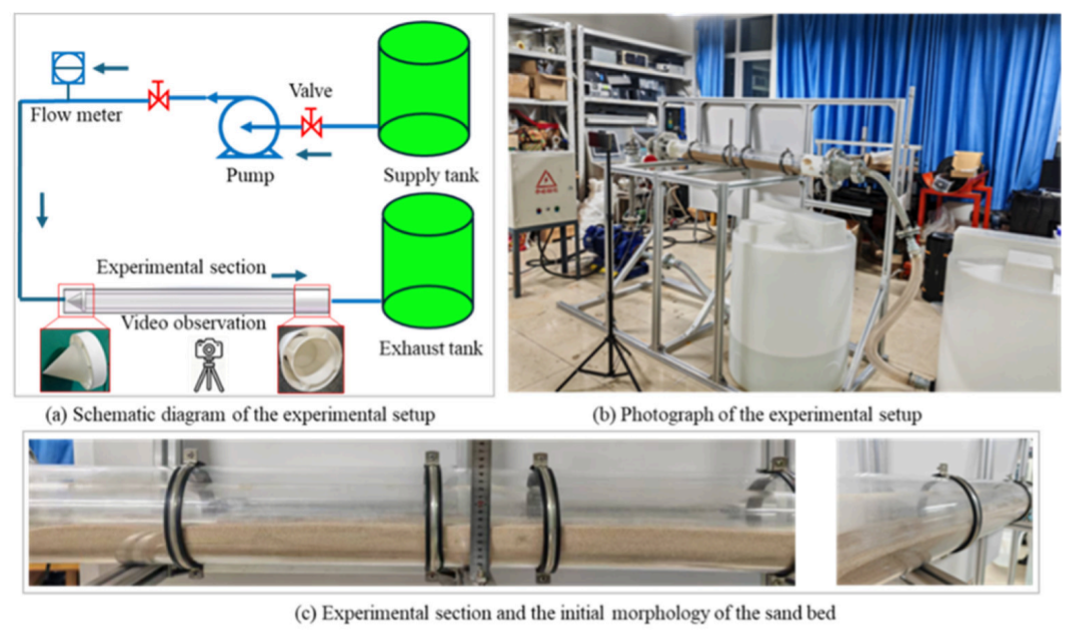
\includegraphics[width=0.9\textwidth]{figure/chapter2/horizontal-washing-experiment-setup.png}
	\caption{水平井筒环空冲砂模拟实验装置}
	\label{fig:horizontal_washing_experiment_setup}
\end{figure}



实验管段中，导流锥与管撑是确保环空流动稳定与几何精度的关键结构组件。导流锥安装于实验管段入口处，其前端锥形结构能够平顺引导流体，有效抑制入口复杂流态。导流锥后端的八个径向格栅是其整流结构的关键组成部分，不仅增强了内管的径向定位刚度，还将流体分割为多股均匀流束，有效促进动量分布均匀化，抑制大尺度涡旋的生成，从而确保进入实验段的流场在周向与径向上保持稳定、对称。此设计显著强化了整体的导流与均流效果，为实验提供了高度均匀的初始流场，抑制了流动的端面效应。管撑安装于实验管段出口端，具有结构定位与约束作用。管撑内缘与内管外壁配合，外缘与外管内壁固定。其主要作用是在出口端继续保持内外管的同心度，与入口端的导流锥形成两点定位，共同保证整个实验段环空间隙的沿程一致性。此外，管撑设计有轴肩，能够有效限制内管在流体作用或振动下可能产生的轴向窜动，防止实验过程中环空有效长度发生改变，从而保障实验边界条件的恒定。

实验开展前，将已知粒度组成的砂粒铺设于透明管段内部，确保砂床高度均匀一致，再像实验管段注入冲砂液。实验所用砂粒为标准石英砂，其参数如表\ref{tab:sand_params}所示。本文以清水和质量分数0.3\%的胍胶液（等效动力粘度12$\mathrm{mPa}\cdot \mathrm{s}$）作为冲砂液，对砂床运移行为进行分组研究。流量通过泵的运行频率调定，并确保每次实验中流速基本保持稳定。实验中，借助高速相机观测砂床的形态变化；此外，在相机的观测窗口设置一刻度尺（下文称其所在位置为“观测点”），利用该刻度尺定量测量砂床高度随时间的变化，以获取不同流量条件下砂床冲砂形态及运移的变化规律。实验的自变量为环空冲砂液平均流速，因变量为砂床的冲砂形态、运移速度和堆积高度等；实验中严格控制的常量包括环空几何结构、砂粒类型与初始质量、砂床初始铺设形态。

\begin{table}[htbp]
    \centering
    \caption{实验中使用的砂粒参数}
    \label{tab:sand_params}
    \begin{tabularx}{.9\textwidth}{XXc}
        \toprule % 顶部粗线
        参数 & 数值 & 单位 \\
        \midrule % 中间细线
        砾径中值 & 0.25 & mm \\
        砾径标准偏差 & 0.058 & mm \\
        砂砾密度 & 2500 & kg/m$^3$ \\
        砂砾堆积密度 & 1750 & kg/m$^3$ \\
        初始砂床高度 & 75 & mm \\
        \bottomrule % 底部粗线
    \end{tabularx}
\end{table}

\subsection{实验结果与讨论}
\subsubsection{清水冲砂}
水平井筒环空冲砂过程中，砂床的运移与沉积行为受多物理场耦合作用支配，涉及来流流量、流体物性、砂粒体积分数、流道几何约束等多个独立变量。若直接采用传统的数据拟合方法构建多变量经验关联式，不仅需要庞大的实验矩阵支撑，且所得公式往往量纲不一致、缺乏物理可解释性，难以推广至不同几何尺度或流体体系的工况。量纲分析法以Buckingham $\pi$定理为基础，能够将多变量物理问题转化为少数几个独立无量纲数群之间的函数关系，可有效约减变量空间，降低实验数据拟合的复杂度，且无量纲数具有明确的物理含义，不仅为从机理层面解释砂床行为的控制因素提供便利，也为实验结果在不同管径尺寸、不同流体体系的冲砂作业中推广奠定基础。鉴于本文实验涉及流量、粘度、砂床高度、运移速度、含砂体积分数等较高变量维度，且实验组数量受限于物理模拟条件，采用量纲分析法进行数据降维与函数关系建构，是实现从有限实验数据中提取普适性规律的合理且必要的技术路径。

在清水组实验中，名义值泵送流量$Q$为实验变量，并分别取$Q=8.5\mathrm{m^3/h}$、$11.8 \mathrm{m^3/h}$、$13.7 \mathrm{m^3/h}$、$15.4 \mathrm{m^3/h}$，用以探究来流情况对砂床运移行为的影响。胍胶液冲砂组旨在探究高粘度冲砂液对砂床运移行为的影响。对于管流，通常用流动雷诺数$Re$对流动性质进行综合表征，即
\begin{equation}
	Re=\frac{\rho U L}{\mu}
\end{equation}

式中，$\rho$和$\mu$分别为介质的密度和动力粘度；$U$为流动的特征速度。在计算泵为实验管段提供的来流雷诺数$Re_{in}$时，$\rho$和$\mu$根据冲砂液的物理属性取值；特征长度L取为环空的等效水力直径，即环空的内外径之差—$(D_o-D_i )$；特征速度U取为环空平均流速，根据流量$Q$和环空横截面积计算。再定义特征时间$T=(D_o-D_i)/U$，对于给定的时间$t$，可用$t^*=t/T$对其进行无量纲化处理。清水冲砂过程中来流雷诺数$Re_{\mathrm{in}}$随无量纲时间$t^*$的变化情况如图\ref{fig:incoming_Re_variation}所示，实验过程中供液桶水头持续降低等因素导致$Re_{\mathrm{in}}$呈现少量下降趋势，但相对变化量仅为2.83\%、1.72\%、0.81\%、1.31\%，因此，实验过程中的来流仍可视为定常。
\begin{figure}[htbp]
	\centering
	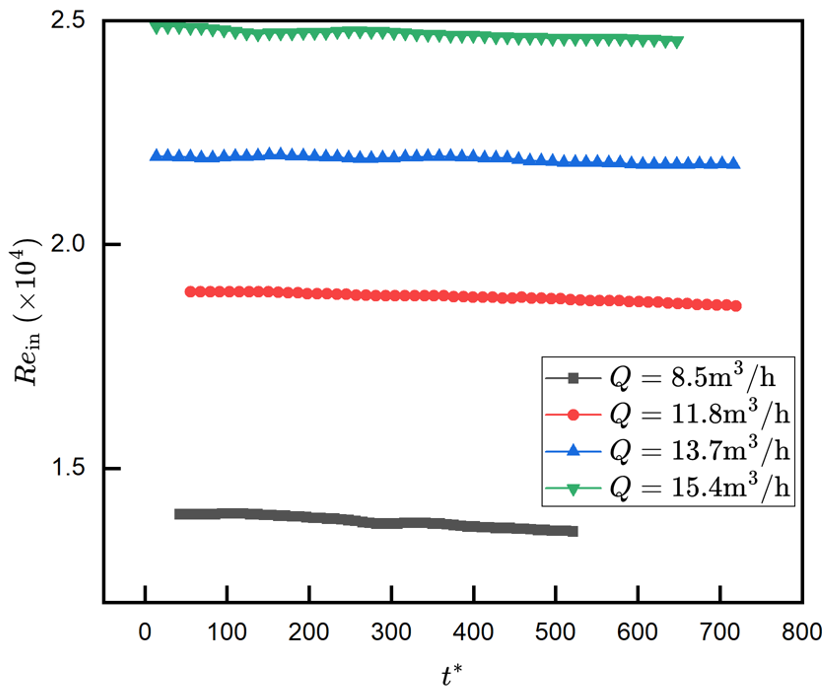
\includegraphics[width=0.7\textwidth]{figure/chapter2/IncomingReVStstar.png}
	\caption{进口雷诺数$Re_{in}$随无量纲时间$t^*$的变化情况}
	\label{fig:incoming_Re_variation}
\end{figure}

为定性描述砂床前缘的变化过程，本文利用拐点、驻点来刻画砂床前缘瞬时轮廓的特征，如图\ref{fig:stagnation_inflection_point}所示。设来流方向为y轴正方向，重力方向为x轴正方向。

\begin{figure}[htbp]
	\centering
	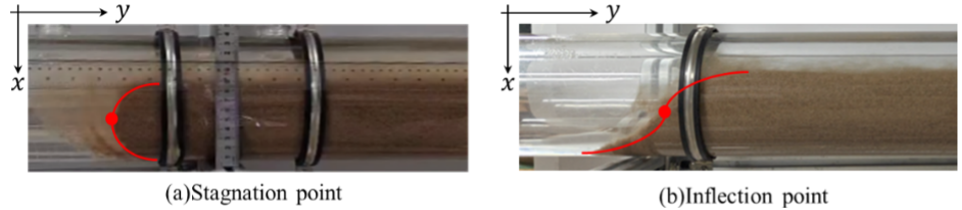
\includegraphics[width=0.7\textwidth]{figure/chapter2/stagenation-with-inflection-point.png}
	\caption{砂床前沿剖面中滞点与拐点的示意图（红色线条旨在示意性展示砂床前沿剖面形态，并不代表精确的定量测量结果）}
	\label{fig:stagnation_inflection_point}
\end{figure}

取来流雷诺数依次为$Re_\mathrm{in}=1.36×10^4 $、$1.89×10^4$ 、$2.20×10^4$三个实验组中砂床的形态变化作为研究对象。冲砂伊始，初始前缘上的砂粒在冲砂液冲击下出现短暂的剧烈翻滚，大量砂粒被扬起，弥散到冲砂液中形成高浓度砂团并随主流向后运移。当砂团经过砂床顶部时，携砂液中的部分砂粒因重力作用再次沉降，导致砂床出现不同程度的局部抬高现象，不同组别的前缘变化过程如图\ref{fig:bed_front_profile_Rein}所示。当砂床前缘呈现稳定状态时，冲砂进入准稳态阶段，但不同组别的前缘在这一阶段呈现出显著差异。

\begin{figure}[htbp]
	\centering
	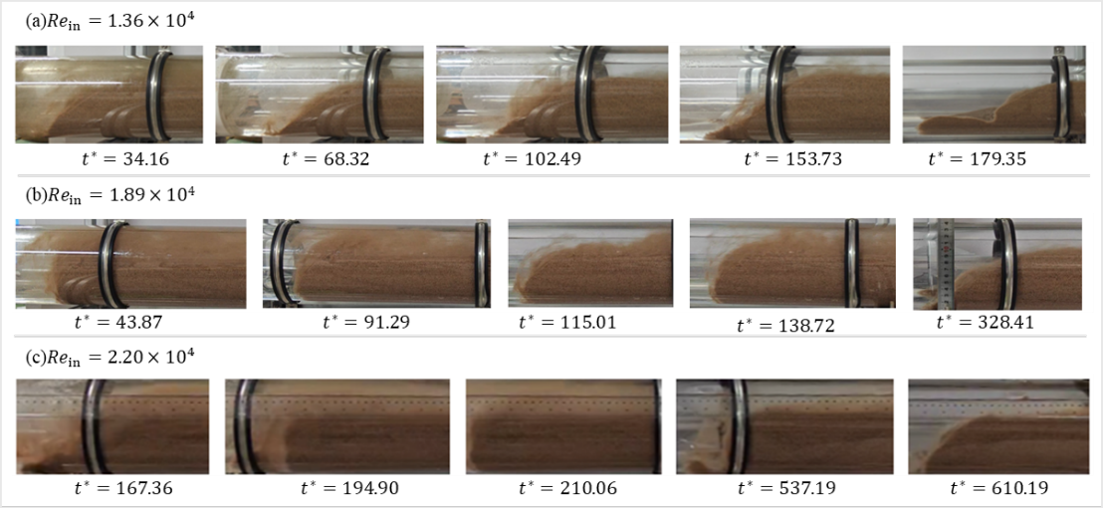
\includegraphics[width=0.7\textwidth]{figure/chapter2/bed-front-profile-VS-Rein.png}
	\caption{来流雷诺数对砂床前缘形态的影响}
	\label{fig:bed_front_profile_Rein}
\end{figure}

在$Re_{\mathrm{in}}=1.36×10^4$实验组（图\ref{fig:bed_front_profile_Rein}（a））中，当$t^*<153.73$时，随时间的推移，砂床前缘不断变瘦削，迎角不断减小。在$t^*=153.73$时，前缘轮廓线出现拐点并进一步产生失稳现象，分蘖成两个高度较小的次生床，这两个床层近似关于管道轴面两侧的平行平面对称分布。随时间的推移，次生床长度不断增大。次生床的形成主要由来流对砂床前缘的剪切应力分布不均所致，随着主床迎角的逐渐减小，拐点以下区域的来流剪切应力已不再整体高于砂粒运移阈值，这一临界条件的变化是次生床发育的关键诱因。$t^*>153.73$后，大量砂粒从主床前缘猝发性地卷入主流，在砂床上部形成高浓度携砂云团并随主流向后运移。同时，砂床前缘区域出现明显的边界层分离迹象，且环空顶部流体因流道收缩而流动加速。
在$Re_\mathrm{in}=1.89×10^4$实验组（图\ref{fig:bed_front_profile_Rein}（b））中，进入准稳态冲砂后，砂床前缘出现驻点。驻点以上区域的砂粒受流体剪切作用大量卷入主流，形成高浓度砂团；由于砂床前缘迎角较大，前缘与砂床顶面相交形成尖锐棱角，该几何特征直接诱发边界层分离，使得砂团以翻滚形态向下游运移。而驻点以下的砂粒，在来流的直接冲击下，甚至出现向左上方的逆向运移行为，随后受上部高速主流的阻滞作用逐渐减速，最终转向下游运移（$t^*=43.87$）。值得关注的是，驻点下方砂粒形成的砂团，在砂床上方的空间位置反而高于驻点上方砂粒形成的砂团，呈现出上下位置颠倒的独特现象。此外，砂粒运移呈现边运移边沉积的特征，且砂团与砂床前缘的运移速度均较$Re_\mathrm{in}=1.36×10^4$实验组有显著提升。随着时间的推移，砂床前缘轮廓线上的驻点持续向下迁移，在$t^*=91.29$时驻点消失在管壁上。砂床前缘的迎角随冲砂进行而持续减小。在$t^*=115.01$时，砂床前缘轮廓线出现拐点，在$t^*=328.41$时，进一步发育形成一个高度与长度均较小的次生床。
在$Re_\mathrm{in}=2.20×10^4$实验组（图\ref{fig:bed_front_profile_Rein}（c））中，进入准稳态冲砂后，砂床前缘在来流的冲蚀作用下，产生大量高浓度砂团，并迅速分蘖出次生床。随着冲砂的进行，主床前缘形成驻点，该实验组也出现了与图\ref{fig:bed_front_profile_Rein}（b）相似的砂床前缘上部高浓砂团和砂粒上下颠倒现象。在$t^*=167.39$时开始分蘖次生床，$t^*=194.90$时次生床与主床开始剥离。此后，在来流的冲蚀和来流冲击主床驻点下方砂床而形成的逆向扬起的共同作用下，次生床逐渐弥散在冲砂液中。在$t^*=537.19$时，在来流方向距主床一定距离处，开始出现完全剥离且前缘厚、中后部薄的次生小砂床。在来流流速近似恒定的情况下，前缘顺流区与逆流区共同作用处产生流速极低的空间，未及时运移的砂粒在此堆积，从而形成次生小砂床。


当携砂云团中的部分砂粒在砂床上方发生再沉积时，砂床高度随之抬升；与此同时，环空顶部的过流面积因砂床高度抬升而减小，流体在收缩流道内流动加速，强化了砂层运移，二者交替作用形成了独特的周期性动力振荡模式。图\ref{fig:bed_oscillation}为清水冲砂一个振荡周期内砂床运移的典型图示，砂团的形成和输运交替进行：第一个子图对应砂粒运移的镇静期，此时携砂云团或已沉降，或已运移至观测视野之外，砂床表面暂未出现大规模砂粒起动现象；第二个子图为携砂云团的生长期，大量砂粒从主床前缘被流体猝发式扬起，即将沿主流向后运移，主床前缘形态因砂粒起动而趋于模糊，但砂床顶部的轮廓仍保持清晰；第三个子图砂团在整个砂床表面呈现非均匀运移特征；第四个子图砂粒运移活动趋于停止，系统恢复至镇静状态。
\begin{figure}[htbp]
	\centering
	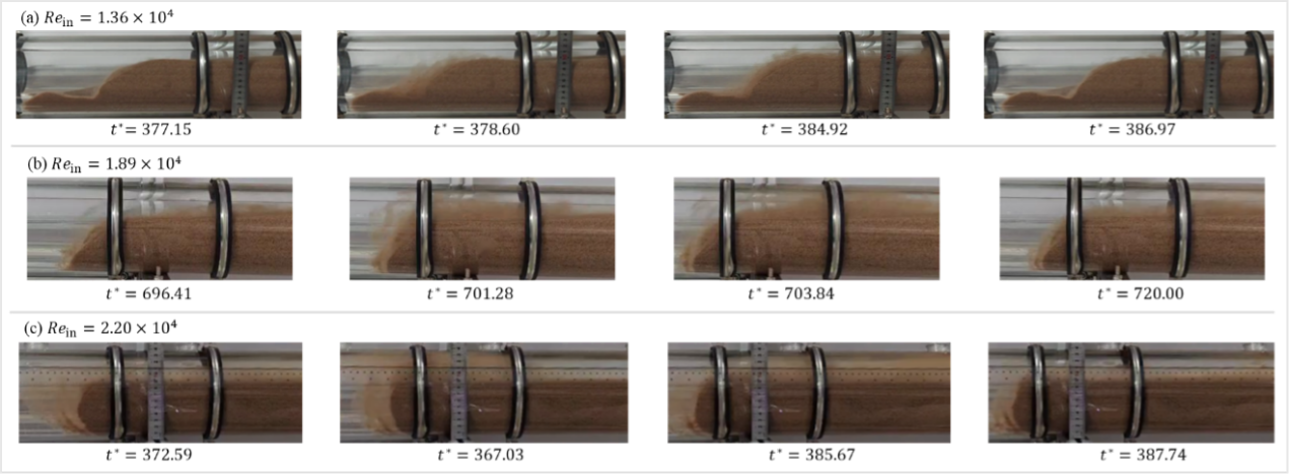
\includegraphics[width=0.7\textwidth]{figure/chapter2/bed-oscillation.png}
	\caption{清水冲砂中砂床运移的自激振荡现象}
	\label{fig:bed_oscillation}
\end{figure}

观测点处的砂床无量纲高度$h^*$随冲砂时间$t^*$的变化曲线呈现近“M”形，如图\ref{fig:M_shaped_bed_height}所示。以$Re_{\mathrm{in}}=1.36×10^4$组为例，在$t^*<200$时，砂床前端砂粒随主流向后运移，并在砂床顶部形成堆积，砂床高度明显升高。在$200<t^*<400$时，管壁的几何约束促使边界层实现再附着，观测点处流体不仅流速较高，还存在较大的向下速度分量，进而对砂床顶部施加显著的剪切应力，加速砂粒的侵蚀与流失，使得砂床高度呈现持续降低的演变趋势。在$400<t^*<500$时，砂床高度采样点的分布特征转为上凸形态，边界层分离点附近形成的逆压梯度，导致砂粒运移动能衰减并发生局部沉积。在运移的末期，即$t^*>500$时次生床长度持续拉长，主床前缘迎角已降至极小值，整体近似呈现流线型形态。
\begin{figure}[htbp]
	\centering
	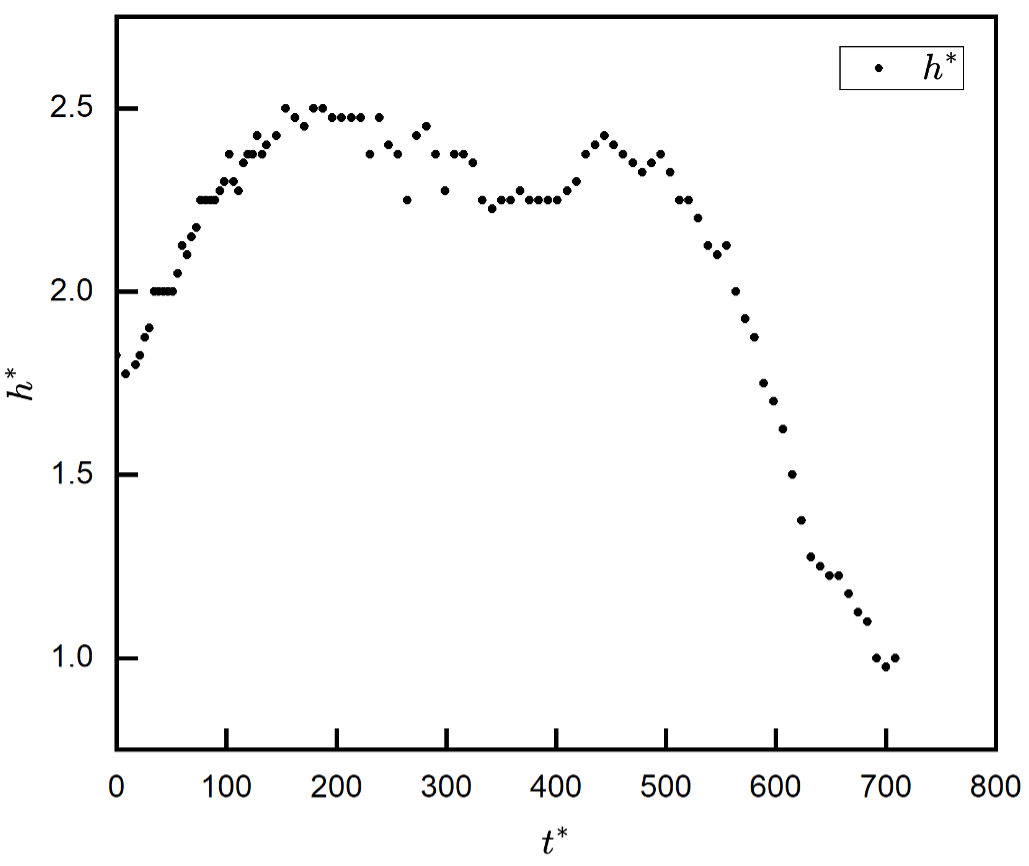
\includegraphics[width=0.7\textwidth]{figure/chapter2/M-shaped-bed-height.png}
	\caption{观测点处砂床高度随时间变化情况（$Re_{\mathrm{in}}=1.36×10^4$）}
	\label{fig:M_shaped_bed_height}
\end{figure}

砂床整体运移行为表明，由于砂粒尺寸细小且表面存在细微锐边，使得砂床堆积密实，同时与管道壁面形成显著的摩擦及锚定效应，进而产生较强的颗粒间内摩擦力与管壁摩擦力。砂床整体不发生迁移或滑移，以近似刚体状态与管道壁面保持相对静止。这一物理现象是绝大多数基于欧拉方法的数值模拟难以精准捕捉的，其核心原因在于砂粒初始堆积浓度过高，导致欧拉方法成立的前提假设难以满足，这也对新型模拟算法的开发提出了迫切需求。
\subsubsection{胍胶液冲砂}
胍胶液冲砂实验过程与清水冲砂相似，实验前调配一定浓度的胍胶增粘液，并在实验开始前使用粘度计测定其粘度。图\ref{fig:eta_gamma}中的流变测试结果表明：当剪切速率低于$720 \mathrm{s}^{-1}$时，胍胶液的表观粘度随剪切速率增加而降低，呈现出符合幂律模型[25]的典型剪切稀化现象。
\begin{equation}
	\eta=K\cdot \gamma^n
\end{equation}

\begin{figure}[htbp]
	\centering
	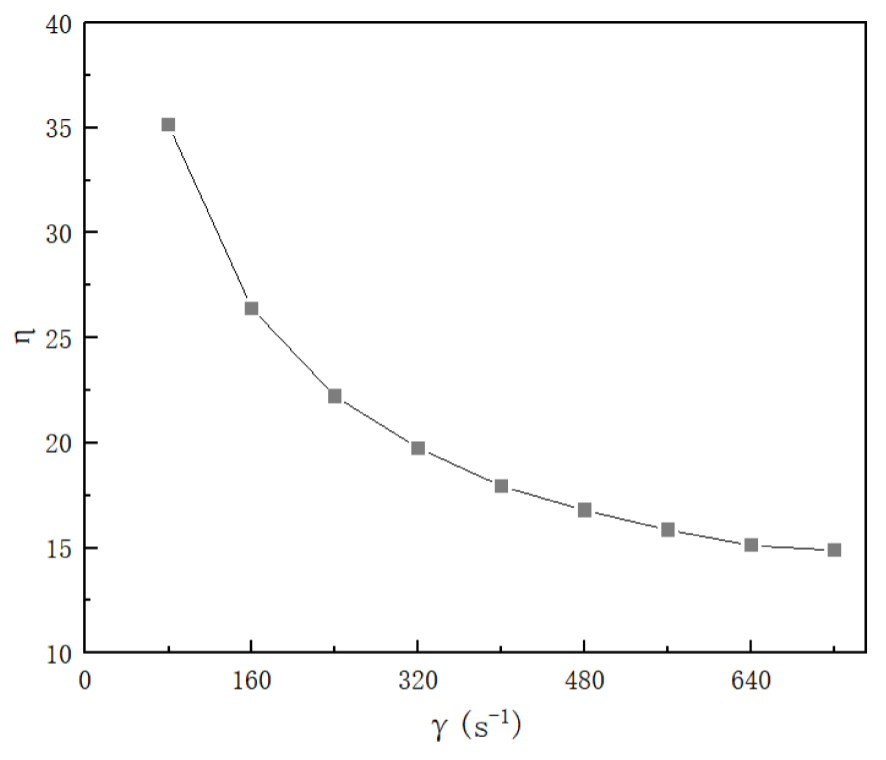
\includegraphics[width=0.7\textwidth]{figure/chapter2/eta-gamma.png}
	\caption{瓜尔胶的粘度-剪切速率关系}
	\label{fig:eta_gamma}
\end{figure}
将数据代入方程可得$\eta=22.53\cdot \gamma^{0.9764}$，对$80$–$720 \mathrm{s}^{-1}$范围内的数据进行了幂律拟合，其拟合优度$R^2=0.9946$。根据Metzner–Reed相关性，幂律流体流动的广义雷诺数可表示为

\begin{equation}
	Re_{\mathrm{MR}}=\frac{\rho V^{2-n} D^n}{K \left(\frac{3n+1}{4n}\right)^n\cdot 8^{n-1}}
\end{equation}

胍胶液的密度近似等于水的密度。将相关数据代入公式(2)后，可得出广义雷诺数约为 $Re_\mathrm{g}=2.048×10^3$，该值接近层流向湍流转变的临界值。

胍胶液冲砂组的来流雷诺数为$Re_\mathrm{g}=2.048×10^3$，处于弱湍流状态且携砂能力相对较弱，这与清水冲砂组情况有明显差异，图\ref{fig:bed_profile_guar_gel}为胍胶液组砂床前缘变化过程。$t^*<570.51$时，环空内仅在砂床前缘整形阶段产生了大范围高浓度砂团，随着冲砂的持续，砂床前缘不断瘦削并分蘖出次生床。$t^*=570.51$时，次生床运移速度追赶上主床，并与之融为一体。此后主床前缘迎角持续下降，冲砂液在砂床前缘携带砂粒向后呈现非均匀运移，在持续的冲砂作用下，砂床前缘逐渐平整，整个砂床轮廓趋于流线型。此阶段为冲砂的主要发生阶段，也是砂床前缘塑形的关键阶段。至$t^*=871.79$，砂床前缘及顶部轮廓已逐渐变为流线型，迎角持续降低，砂床形态变得更加瘦削，砂粒随主流向后呈均匀运移状态。至$t^*=1102.56$冲砂结束时，砂床整体呈现流线型。本组实验中并未出现明显的自激振荡现象。

\begin{figure}[htbp]
	\centering
	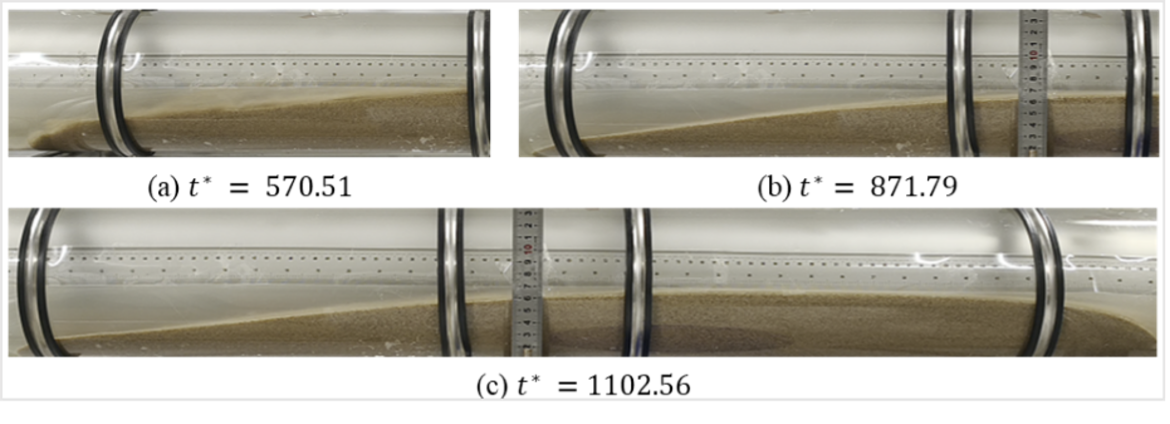
\includegraphics[width=0.7\textwidth]{figure/chapter2/bed-profile-guar-gel.png}
	\caption{观测点处砂床高度随时间变化情况（$Re_{\mathrm{in}}=1.36×10^4$）}
	\label{fig:bed_profile_guar_gel}
\end{figure}

在清水组和胍胶液组的准稳态运移阶段，砂床顶部的流动均表现出显著的分层运移行为，且这种分层特征在轴向远离前缘的区域尤为典型。具体可划分为两层：远离砂床顶部的流道是对流层，砂粒体积分数较低，分布范围较大，受主流拖拽作用显著，运移速度较快；靠近砂床顶部的是剪切滑移层，受床面剪切作用主导，砂粒体积分数较高，颗粒间相互作用强烈，运移速度较慢。测量剪切滑移层厚度发现，$Re_{\mathrm{in}}=1.36×10^4$组中厚度约为6.0mm，$Re_{\mathrm{in}}=1.89×10^4$组中约为6.2mm，$Re_{\mathrm{in}}=2.20×10^4$约为6.8mm，三组数值差异较小；相比之下，胍胶液组剪切滑移层厚度约为3.5mm，较清水组减小约45.0\%，表明在实验中清水对砂床的整体剪切作用高于胍胶液。

\subsubsection{砂床运移行为的控制因素分析及讨论}

本文基于室内实验观测现象与数据处理结果，构建表征砂粒运移行为特征的数学模型。实验数据解析以量纲分析为核心方法，从工程应用角度出发，砂粒运移速率与砂床堆积高度为冲砂洗井作业过程中的核心特征参数，因此将其作为后续数学模型的输出变量；模型输入变量则选取冲砂液粘度、密度及冲砂排量等工艺与水力关键参数。

本文假设在不同实验组中，沙床运移稳定后，砂头的速度$V_\mathrm{s}$与砂床堆积高度$h$基本不受砂床初始形态及初始高度的影响。砂头运移速度$V_\mathrm{s}$主要受控于来流流动条件，上文已用来流雷诺数$Re_{\mathrm{in}}$对其流动特征进行表征，$V_\mathrm{s}$对应的特征速度可取环空平均流速$U_\mathrm{in}$。相比之下，砂床堆积高度$h$的影响机制更为复杂，主要由砂床抬升所引发的流道堵塞效应主导，其演化受含砂液流的冲刷剪切作用与砂粒重力沉降作用共同耦合控制。在重力场恒定条件下，砂粒沉积效应主要与砂体积分数$\varphi_\mathrm{s}$及局部流速$U_\mathrm{l}$密切相关；而含砂液的剪切作用则取决于局部流速速$U_\mathrm{l}$、等效黏度$\mu_{\mathrm{eq}}$与等效密度$\rho_{\mathrm{eq}}$，可选取砂床顶部流道内的流动雷诺数$Re_\mathrm{l}$作为表征砂床堆积效应的综合评价指标。$Re_\mathrm{l}$与流体含砂量密切相关，根据流动连续性方程，流道中砂体积分数$\varphi_\mathrm{s}$与砂头运移速度$V_s$存在内在关联；同时，砂床抬升所引发的堵塞效应并非局部现象，也受砂床运移速度$V_\mathrm{s}$的制约。因此，在构建砂床高度的数学模型时，应充分纳入砂头运移速度$V_\mathrm{s}$的影响。综合上述，需要找到以下两个关系

\begin{equation}
    \begin{cases}
        V_s^* = V_s^*(Re_{\mathrm{in}}) \\
        Re_1 = Re_1(Re_{\mathrm{in}})
    \end{cases}
\end{equation}

实验中定量测得的砂头位置随时间的变化关系如图\ref{fig:p_star_VS_t_star}所示，图中以来流流量$Q$为参数。图中砂头的无量纲位置$p^*$是用砂头的实际位置与内外管径之差($D_o-D_i $)进行无量纲化后得到的；无量纲时间$t^*$是实际观测时间$t$用特征时间$T=(D_o-D_i)/U_in$进行无量纲化得到的。从图\ref{fig:p_star_VS_t_star}中可以看出，在准稳态运移阶段，$p^*$和$t^*$之间呈现线性变化规律。用线性函数对$p^* $($t^* $)进行拟合，可得砂头的无量纲运移速度$V_s^*$，图\ref{fig:Vs_star_VS_Rein}展示了$V_s^*$随$Re_{\mathrm{in}}$的变化情况，可见二者也近似呈现线性关系。用线性函数进行拟合得

\begin{figure}[htbp]
	\centering
	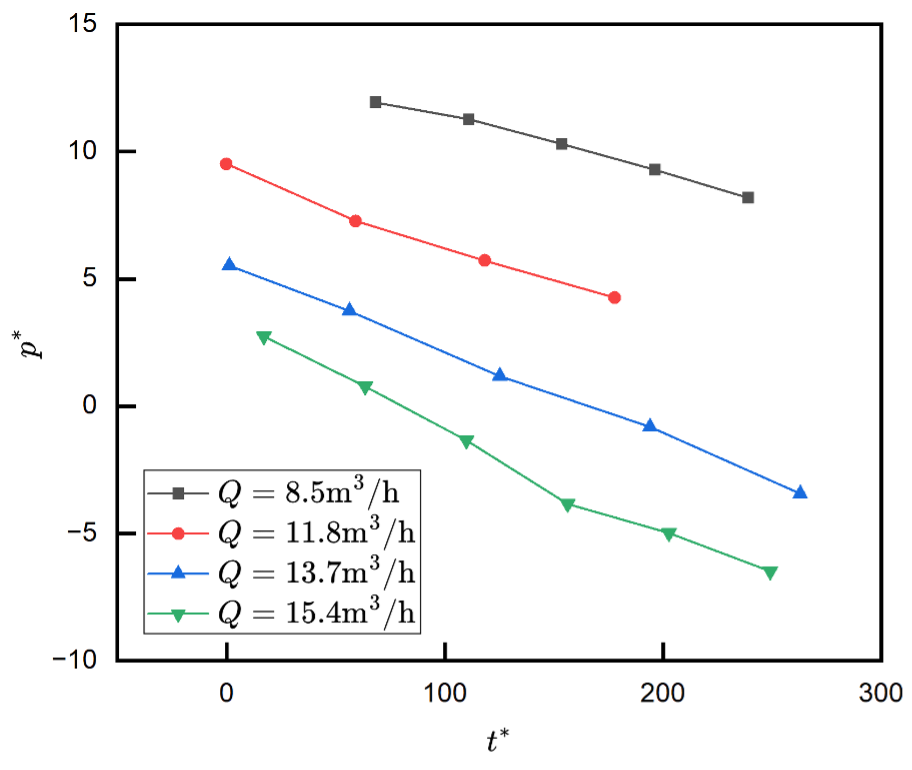
\includegraphics[width=0.7\textwidth]{figure/chapter2/p-star-VS-t-star.png}
	\caption{砂头位置$p^*$与冲砂时间$t^*$的变化关系}
	\label{fig:p_star_VS_t_star}
\end{figure}

\begin{figure}[htbp]
	\centering
	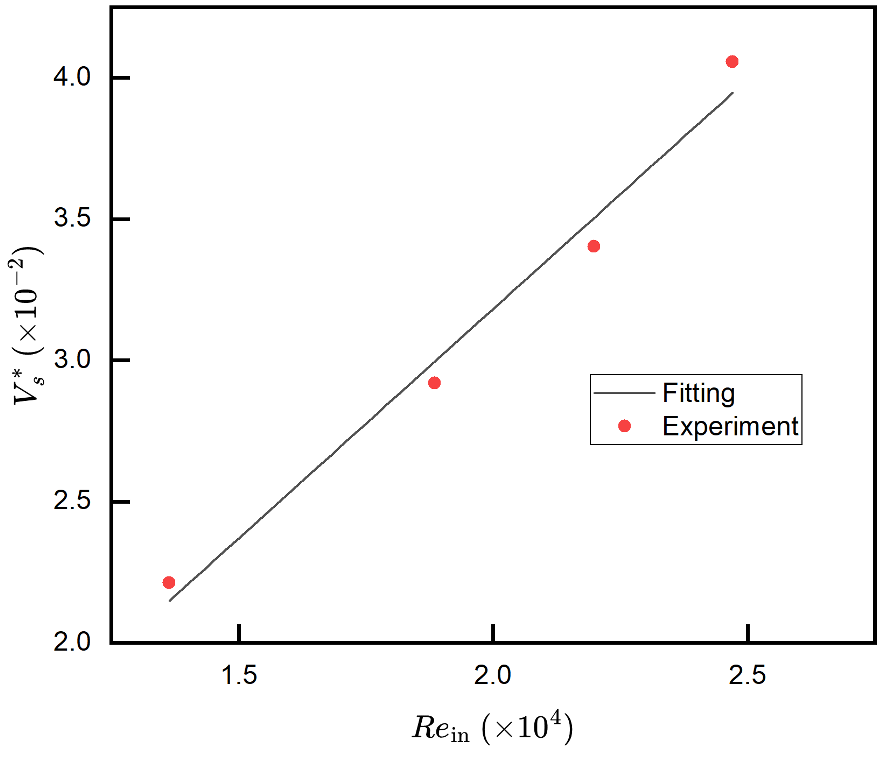
\includegraphics[width=0.7\textwidth]{figure/chapter2/Vs-star-VS-Rein.png}
	\caption{砂头运移速度$V_s^*$与进口雷诺数$Re_in$之间的关系}
	\label{fig:Vs_star_VS_Rein}
\end{figure}

\begin{equation}
	V_s^* = (1.62 \times 10^{-4} Re_{\text{in}} - 0.067) \times 10^{-2} \approx 1.62 \times 10^{-6} Re_{\text{in}}
\end{equation}

可见，$V_s^*$与$Re_{\mathrm{in}}$近似成正比例关系。

此外，实验中测量了由($D_o-D_i $)进行无量纲化无量纲最大高度$H^*$，其与$Re_\mathrm{in}$之间的变化关系如图\ref{fig:Rel_VS_Rein}所示；再根据流道几何计算局部雷诺数$Re_l$，其与$Re_\mathrm{in}$之间的变化关系如图\ref{fig:H_star_VS_Rein}所示。对于$Re_l$的计算，式（1）对应的当地参数取法为：$U$是砂床顶部通道中的平均流速，$ρ$是携砂液的平均密度，特征长度需选为流动通道的水力直径，计算表达式为$L=4S⁄P$，其中，$P$是润周，$S$是过流截面面积。根据实验中观测的现象，可做合理假设：砂床的上顶面是水平面，可结合砂床的高度H和几何关系计算$P$。此外，洗井液含砂后会对等效密度和粘度产生显著影响，本文采用砂粒的体积分数$ϕ_s$作为基础参数定量表征洗井液含砂的影响，$\varphi_s$的计算可根据砂头的位移速度$V_s$、砂床的高度$H$和来流流量$Q$进行。由于流动通道中流速较快，实验中观测到流道中砂的浓度稀薄，含砂液与纯水的相对粘度$\mu_r$可按下式计算
\begin{equation}
	\mu_r= 1+2.5\phi _s
\end{equation}

\begin{figure}[htbp]
	\centering
	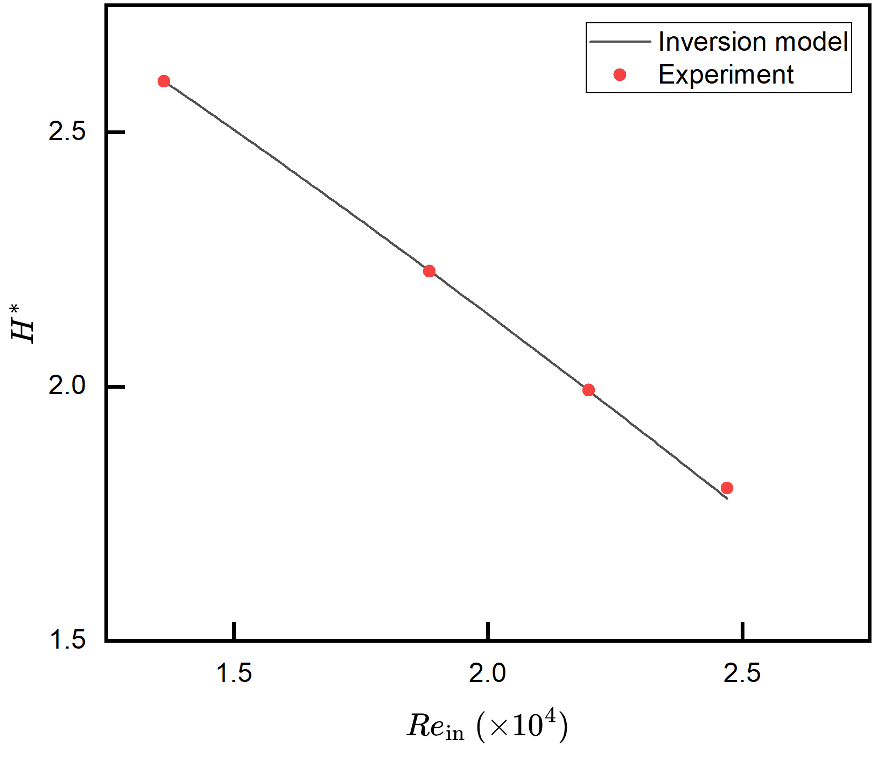
\includegraphics[width=0.7\textwidth]{figure/chapter2/H-star-VS-Rein.png}
	\caption{砂床最大高度$H^*$与来流雷诺数$Re_in$的关系}
	\label{fig:H_star_VS_Rein}
\end{figure}

\begin{figure}[htbp]
	\centering
	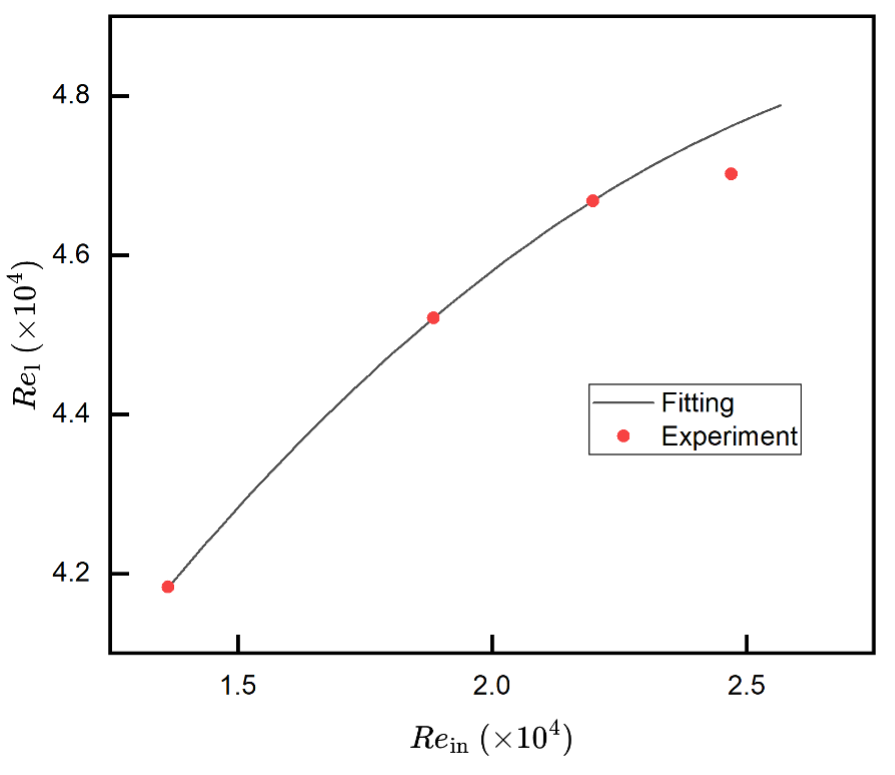
\includegraphics[width=0.7\textwidth]{figure/chapter2/Rel-VS-Rein.png}
	\caption{局部雷诺数$Re_l$与来流雷诺数$Re_\mathrm{in}$之间的关系}
	\label{fig:Rel_VS_Rein}
\end{figure}

$Re_l$和$Re_\mathrm{in}$之间的变化关系如图\ref{fig:Rel_VS_Rein}所示。随着$Re_\mathrm{in}$的增加，$Re_l$呈现单调递增的趋势。对前三组数据用二次函数进行拟合，第四组数据作为验证，可得
\begin{equation}
	Re_1 = -2.138 \times 10^{-5} Re_{\text{in}}^2 + 1.344 Re_{\text{in}} + 2.748 \times 10^4
\end{equation}
其中，第四组实验数据的相对误差为1.28\%，表明二次拟合模型在当前实验条件下充分捕捉了$Re_l$和$Re_\mathrm{in}$之间的关系。综上所述，方程(7)适用于来流雷诺数范围从$1.36×10^4$增至$2.47×10^4$且砂粒参数如表1所示的情况。

在实验数据的支撑下得到式(7)的关系后，可反解出$H^*$和$Re_{\mathrm{in}}$之间的关系。由于$H$和$S$在几何约束下呈非线性函数，所以$H^*$和$Re_in$是一个隐函数关系。本文通过数值方法求解得到了$H^*$的数值解，如图11所示，第四组实验中的$H^*$预测相对误差为$1.15\%$，预测精度较高。从拟合曲线的形状可以看出，$H^*$与$Re_{\mathrm{in}}$二者近似成线性关系，$V_s^*$产生显著变化时对$H^*$的影响较小，其主要原因是砂床的运移绝对速度低，局部流道中砂粒的体积分数较低，而砂粒的重力沉积作用相对较强。

从图\ref{fig:Vs_star_VS_Rein}中可以看出，砂头的无量纲运移速度较低，在4.0\%以下，表明水平段自然冲砂效率很低。砂床的消散动力主要依靠湍流来流的雷诺应力，其剪切分量导致了砂床表层砂粒的滑移及失稳，这种冲砂方法依赖于来流的脉动性；同时，砂粒间连接松散，雷诺应力中正应力分量的不均匀分布，会导致砂床结构破坏。后者在水平管道冲砂中占据主导地位，在这种冲砂机制下，砂头的形状会被重新塑造，迎角不断减小。在准稳态运移阶段，较小的砂头迎角限制了冲砂能力。若能有一种机制不断改变来流的冲砂方向，破坏锁死的条件，则有可能优化冲砂效率

虽然冲砂液扫除了砂头上游的分散砂粒，但在砂头后方产生了富集，导致砂床高度显著抬升，如图\ref{fig:H_star_VS_Rein}所示。如果在冲砂过程中拖动管柱，有可能导致管柱砂卡风险甚至比冲砂之前还要高。这种现象的主要原因是来流的速度方向和砂粒的重力沉积方向的差异，在水平井中这种沉积效应最为显著。如果在冲砂管柱上安装稳定器以改变流速方向，则有助于改善砂床在水平段的沉积。局部砂床的最大抬高高度随来流雷诺数线性递减，为减小管柱的砂卡风险，可采用增大泵送排量、使用高密度冲砂液等措施优化冲砂过程。

砂床顶部携砂液的雷诺数$Re_l$显著高于来流雷诺数$Re_{\mathrm{in}}$，这种效应主要是过流截面减小所致，而携砂液含砂量变化的影响较小。实际上，在所有实验组中，含砂率均处于较小范围（如图\ref{fig:phis_VS_Rein}所示），这意味着在更高的泵送排量下，局部通道中的流动湍动能越强，对砂床顶部的冲蚀能力和抵抗砂粒重力沉积的效应均越显著。若将实验结果向更高来流雷诺数进行外推，在砂床完全无抬高的极限情况下，局部雷诺数和来流雷诺数应为1:1的关系。考虑到图11中显示的砂床高度随来流雷诺数线性递减，节流形成的加速效应将迅速衰减。在更高的流量下，砂床的沉积效应将消失。可见，泵的排量对冲砂过程起到决定性作用。如果冲砂排量受限于设备的输出能力，也应按照实验结果，将砂床沉积高度控制在安全阈值以下。例如，工程中常将0.3倍以下的砂床高度视为安全，0.4倍以上视为高风险区。

\begin{figure}[htbp]
	\centering
	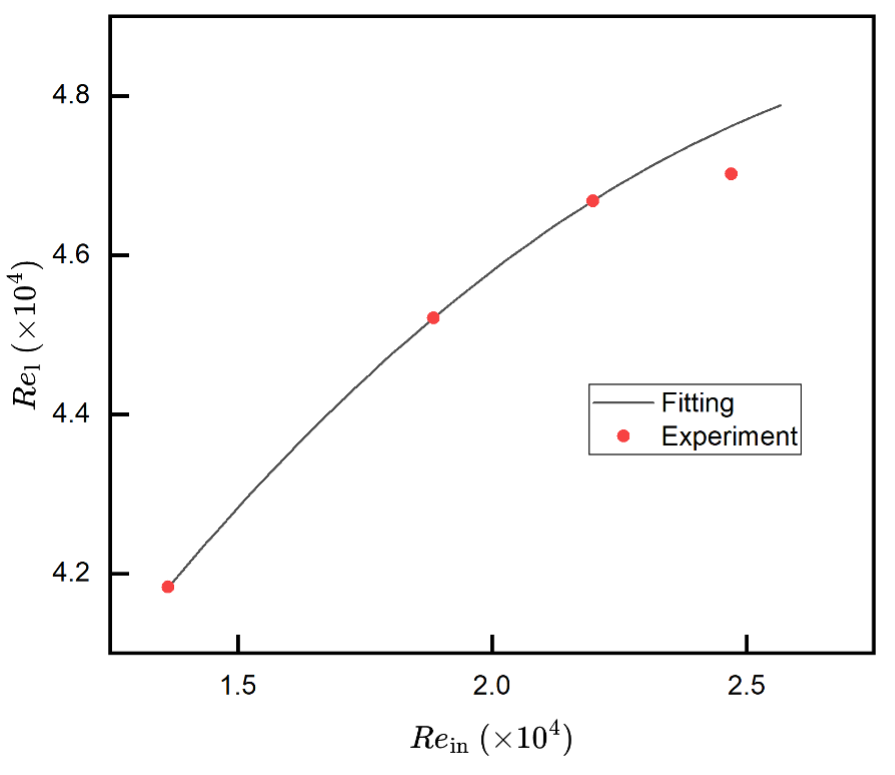
\includegraphics[width=0.7\textwidth]{figure/chapter2/Rel-VS-Rein.png}
	\caption{流道中含砂量$\phi_s$与$Re_{\mathrm{in}}$之间的反演关系}
	\label{fig:phis_VS_Rein}
\end{figure}


冲砂作业过程中，原本沿管柱相对分散分布的砂粒在局部管段出现高度聚集，而管柱及井下工具外表面存在的沟槽、台阶等结构特征进一步强化了砂粒滞留效应。在管柱拖动过程中，上述富集砂体极易引发工具遇卡，影响施工连续性。此外，在低流量冲砂条件下形成的次生砂床，以及高粘度冲砂条件下形成的流线型砂床，易在井下工具或管柱几何变径部位残留，形成连续或间断的沉积带，且这类沉积带难以被后续流体有效冲蚀运移，提高了现场施工作业的安全风险。此外，由于本文提出的物理模型是以无量纲数为研究对象的，其结果具有一定的普适性。该发现在工程中具有重要应用价值，对于水平井筒严重出砂的情况，可根据当地雷诺数估计砂床抬高后的高度，为拖动工具和管柱的砂卡风险定量评估提供依据。

夏齐[21]观察到，在水平井筒内的厚砂层表面颗粒在剪切力和冲击力作用下会通过跳跃和滚动方式向前迁移，这与本文的实验观测结果一致。然而当系统进入准稳态后，砂砾运移模式主要转变为以剪切滑动为主，以滚动运移为辅助。颗粒沉降导致的局部床层隆起现象进一步验证了洪贯洲[22]的CFD-DEM研究结论。将清水冲砂实验组对照发现：对于相同流体条件，湍流强度高，冲砂液携砂运输能力强砂床前缘运移速度快。此外，通过使用胍胶液进行冲砂实验发现，清水相较于胍胶液，具有更优异的冲砂性能。这一发现打破了“高粘度即高效”的传统观点，间接表明流体粘度与冲砂效率之间的关系并非简单的线性关系。本研究通过设置导流锥与管撑以消除环空偏心问题，即在理想同心环空条件下进行冲砂实验；未来将根据现场实际工况进行进一步实验，例如针对偏心工况下的洗砂效果开展深入研究。

本文基于自主设计的水平井筒环空冲砂模拟实验装置，以清水和质量分数0.3\%的胍胶液为冲砂介质，在不同来流流量工况下开展了室内环空冲砂物理模拟实验，系统观测了砂床前缘形态演化、自激振荡及分层运移等动态行为；在此基础上，采用量纲分析法，以来流雷诺数$Re_{\mathrm{in}}$为全局控制参数、局部雷诺数$Re_l$为桥梁变量，构建了砂头无量纲运移速度$V_s^*$与砂床最大堆积高度$H^*$的预测模型，得到以下主要结论：

（1）水平井筒环空内的冲砂过程具有显著的流速依赖性。清水冲砂条件下，随来流雷诺数$Re_in$从$1.36×10^4$增至$2.20×10^4$，砂床前缘依次经历拐点失稳、驻点形成、次生床分蘖与剥离等流态，并伴生由砂床抬升与流道收缩交替作用所引发的自激振荡现象；相比之下，胍胶液冲砂组（$Re_g=2.048×10^3$）处于弱湍流状态，携砂能力弱于清水组，前缘形态趋于流线型，未出现明显自激振荡现象。

（2）砂床顶部流动呈现显著分层特征，可划分为对流层与剪切滑移层。清水三组实验中，剪切滑移层厚度在6.0-6.8 mm之间，且随$Re_{\mathrm{in}}$增加而小幅增大；胍胶液组滑移层厚度约为3.5mm，较清水组减小约45.0\%，表明高粘度流体对床面的剪切作用更弱。

（3）砂头无量纲运移速度$V_s^*$处于极低水平（<4.0\%），表明水平段自然冲砂效率低下。$V_s^*$与$Re_in$呈良好正比例关系。砂床的最大无量纲堆积高度$H^*$随$Re_in$的增加近线性递减，其控制机制主要为流道收缩引发的局部加速效应，而含砂体积分数的影响较小。

（4）通过量纲分析构建了局部雷诺数$Re_l$与来流雷诺数$Re_in$的二次函数模型，验证误差为1.28\%，并可据此隐式求解砂床最大堆积高度$H^*$，预测误差为1.15\%，为工程中评估砂床抬高后的管柱砂卡风险提供了定量方法。

本研究从现象观测走向机理提炼，从定性描述走向定量表征，为严重出砂水平井的冲砂排量优选与砂卡风险评估提供了物理依据与分析工具。后续研究可在本文建立的方法框架上进一步拓展模型维度，发展高保真数值模拟与现场数据同化方法，最终形成从机理认知到工程决策的完整闭环，为复杂油气井修井作业的安全高效实施提供更为坚实的理论基础与技术支撑。

参考文献
1.	Wicks, M. Transport of Solids at Low Concentration in Horizontal Pipes. In Advances in Solid–Liquid Flow in Pipes and Its Application; 1971; pp. 101–124. 
2.	King, M.J.S.; Fairhurst, C.P.; and Hill, T.J. Solids Transport in Multiphase Flows—Application to High-Viscosity Systems. ASME. J. Energy Resour. Technol. 2001, 123, 200–204. 
3.	李明忠, 王卫阳, 何岩峰, 等. 垂直井筒携砂规律研究[J]. 石油大学学报: 自然科学版, 2000, 24(2): 4.
4.	李明忠, 王卫阳, 赵国景. 垂直井筒井液携砂流动规律研究及其在油井生产中的应用[J]. 实验力学, 2002(03): 385-392.
5.	王治中, 邓金根, 孙福街, 等. 井筒砂粒运移规律室内模拟实验研究[J]. 石油学报, 2006(04): 130-132+138.
6.	苏健鹏. 水平-竖直集气管道砂沉积规律与携砂特性研究[D]. 青岛: 中国石油大学(华东), 2019.
7.	Danielson, T.J. Danielson, Thomas J. Sand Transport Modeling in Multiphase Pipelines. In Proceedings of the Offshore Technology Conference, Houston, Texas, USA, 30 April-3 May 2007. 
8.	Zeinali, H. Effect of Near-Wall Turbulence on Selective Removal of Particles from Sand Beds Deposited in Pipelines. Ph.D. University of Alberta, Edmonton, Alberta, AB, Canada, 2012.
9.	侯学文. 水平井冲砂作业砂液两相流动与沉降特性研究[D]. 湖北: 长江大学, 2024.
10.	Archibong-Eso, A.; Aliyu, A.M.; Yan, W.; Okeke, N.E.; Baba, Y.D.; Fajemidupe, O.; Yeung, H. Experimental Study on Sand Transport Characteristics in Horizontal and Inclined Two-Phase Solid–Liquid Pipe Flow. J. Pipeline Syst. Eng. Pract. 2020, 11, 04019050.
11.	Doan, Q.T.; Doan, L.T.; Farouq Ali, S.M.; Oguztoreli, M. Sand Deposition inside a Horizontal Well—A Simulation Approach. J. Can. Pet. Technol. 2000, 39(10).
12.	Najmi, K. Particle Transport in Single-Phase and Multiphase Horizontal Pipes with Emphasis on the Effect of Viscosity; The University of Tulsa,Tulsa, Oklahoma, USA, 2015.
13.	Piroozian, A.; Ismail, I.; Yaacob, Z.; Babakhani, P; Ismail, A. Impact of Drilling Fluid Viscosity, Velocity and Hole Inclination on Cuttings Transport in Horizontal and Highly Deviated Wells. J. Pet. Explor. Prod. Technol 2. 2012 :149-456.
14.	Sorgun, M. Simple Correlations and Analysis of Cuttings Transport with Newtonian and Non-Newtonian Fluids in Horizontal and Deviated Wells. ASME. J. Energy Resour. Technol. September 2013, 135, 032903.
15.	陈珊. 变化水环境中散体沙休止角的初步研究[D]. 武汉: 武汉大学, 2014.
16.	徐进超, 李云, 宣国祥, 等. 船闸泄水作用下引航道中动水冲沙规律[J]. 水科学进展, 2016, 27(02): 186-195.
17.	温庆文. 紫坪铺水库清水下泄河道冲刷演变研究[D]. 雅安: 四川农业大学, 2022.
18.	周双. 推移质泥沙随机起动与输移机理研究[D]. 咸阳: 西北农林科技大学, 2022.
19.	段自豪, 陈杰, 蒋昌波, 等. 非恒定流作用下的推移质泥沙输移实验研究[J]. 中国科学：技术科学, 2019, 49(11): 1372-1382.
20.	Einstein, H.A. The Bed-Load Function for Sediment Transportation in Open Channel Flows; Tech. Bulletin No. 1026; US Department of Agriculture: Washington, D.C. USA, 1950.
21.	夏齐. 不同粘度液-砂流动规律及携砂性能研究[D]. 湖北: 长江大学, 2024.
22.	洪贯洲. 基于CFD-DEM方法对井筒内岩屑运移过程液固两相流动研究[D]. 黑龙江: 东北石油大学, 2024.
23.	朱娜. 大位移钻井岩屑运移规律与阻卡机理研究[D]. 北京: 中国石油大学(北京), 2022.
24.	Soepyan, F.B.; Cremaschi, S.; Sarica, C.; Subramani, H.J.; Kouba G.E. Solids Transport Models Comparison and Fine-Tuning for Horizontal, Low-Concentration Flow in Single-Phase Carrier Fluid. AIChE J. 2014, 60(1), 76–122.
25.	赵鉴楚,耿强.低聚物非牛顿流体流变参数的确定与流动计算[J].石油化工设计,2026,43(1):6-12+81.


\section{全井筒颗粒运移实验}

 % 水平井冲砂
%	\section{全井筒模型颗粒运移实验}

上一节的水平井固液两相流研究多以砂粒作为典型颗粒物，已能较好地揭示细小颗粒的运移规律。然而，实际油气井工况更为复杂，对于粒径更大或密度更高的异形颗粒，全井段的井斜角变化对固相运移及堆积形态具有显著影响。为此，本研究构建了涵盖造斜段与竖直段的全井筒物理模型，以系统评估复杂颗粒在全井段内的运移特征。

在各类修井碎屑中，大型铁块及橡胶块通常需通过专门的打捞工具取出，而微小粉尘级碎屑易随洗井液循环出井。与之不同的是，修井过程（如套铣作业）产生的金属碎屑形状极不规则且缺乏统一规范，其中尺寸适中的短小卷曲状铁屑在井筒中具有极强的滞留性与破坏力：其高硬度及尖锐边缘极易划伤封隔器胶皮，并对井下工具的内部流道及关键密封面造成严重的冲蚀与机械磨损。因此，本研究选用该类代表性卷曲铁屑作为全井筒冲洗实验的固体颗粒模型，旨在为优化井筒清洁工艺提供更加贴近工程实际的理论依据。

实验所构建的全井筒物理模型台架如图\ref{fig:iron_washing_test_rig}所示。该台架包含竖直段、弯管段及水平段，用于完整表征复杂井眼轨迹下的流体及颗粒运移行为。模型采用双层套管结构，其中内管外径为 $90\text{ mm}$，外管内径为 $130\text{ mm}$，洗井介质仅在内、外管形成的环空内自底端向顶端单向流动。流体循环系统配备了变频驱动泵与控制柜，并利用在线流量计对循环流量进行实时高精度监测。为防止循环流体中的铁屑颗粒对泵体造成冲蚀与磨损，系统采用了“进水-出水双罐隔离”的开式循环防护设计。在实验过程中，通过变频控制逐步缓慢地提升洗井流量（流量平均变化率为$27.12\mathrm{m^3/(h^2)}$），以确保管内流场始终处于准稳态发展历程。此外，实验在竖直段、弯道段及铁屑初始沉积床区域分别建立了3个光学观测窗口，同步采集流量动态数据与各观测点的同帧高速视频，为后续颗粒运移与床面演化的定量图像分析提供数据支撑。

\begin{figure}	
	\centering
	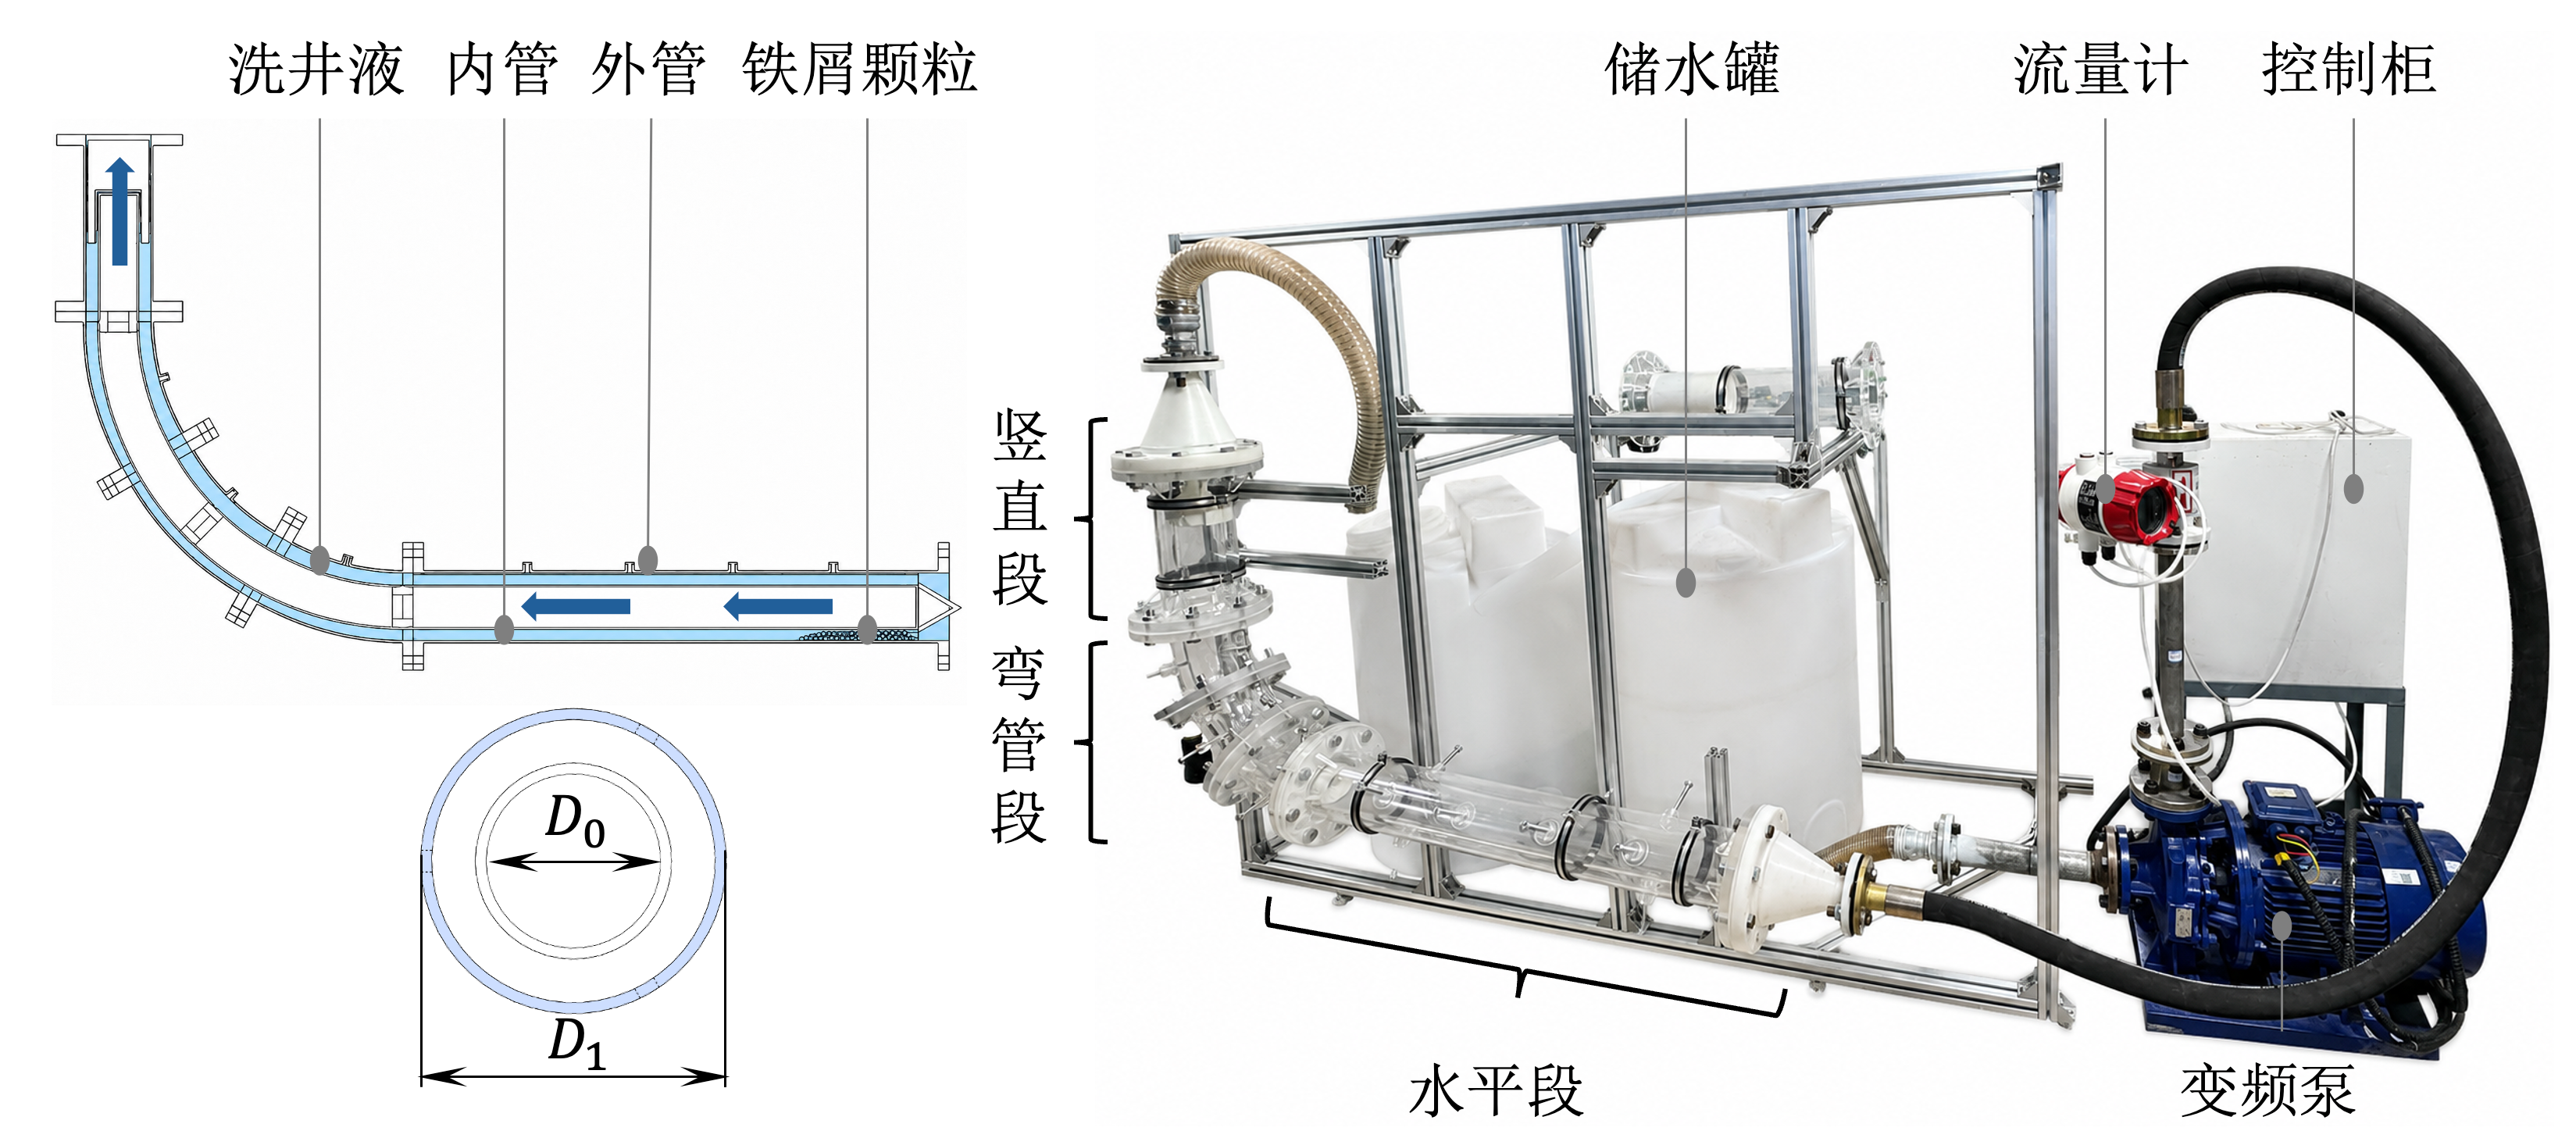
\includegraphics[width=1.\textwidth]{figure/chapter2/iron-washing-test-rig.png}
	\caption{铁屑冲洗实验装置}
	\label{fig:iron_washing_test_rig}
\end{figure}

\subsection{实验结果及讨论}

铁屑床的初始形态如图 \ref{fig:initial_bed_profile} 所示。随着泵流量$Q$的逐步增加，床层的宏观演化过程及流场特征表现出显著的阶段性规律。
当$Q=7.5\mathrm{m^3/h}$ 时，床层内的铁屑颗粒开始呈现运动趋势，部分颗粒自床层前缘起发生向后的位移，标志着床层由静止向流态化转变的初始阶段。当 $Q=10.00\mathrm{m^3/h}$ 时，铁屑床的宏观形态呈现出明显的非均匀拉伸特征：床层上部颗粒的运移距离显著大于下部颗粒。这种沿周向分布的运移差异表明，尽管设置了导流锥，但进口区域的流速分布不均现象尚未被完全消除，局部流场仍存在明显的梯度效应。
随着$Q=11.70\mathrm{m^3/h}$，铁屑床发生显著的宏观位移，其前缘已接近当前观测视野的边界。值得注意的是，在此高流量工况下，床层形态的演化反而表现出更高的均匀性与对称性。这一现象证实，随着流体向下游发展，环空区域的流速分布趋于均匀化，表明本实验系统对来流均匀性的整体控制质量良好，能够满足后续研究的流场要求。
\begin{figure}[htbp]
	\centering
	\subfloat[$Q=7.85\mathrm{m^3/h}$]{%
	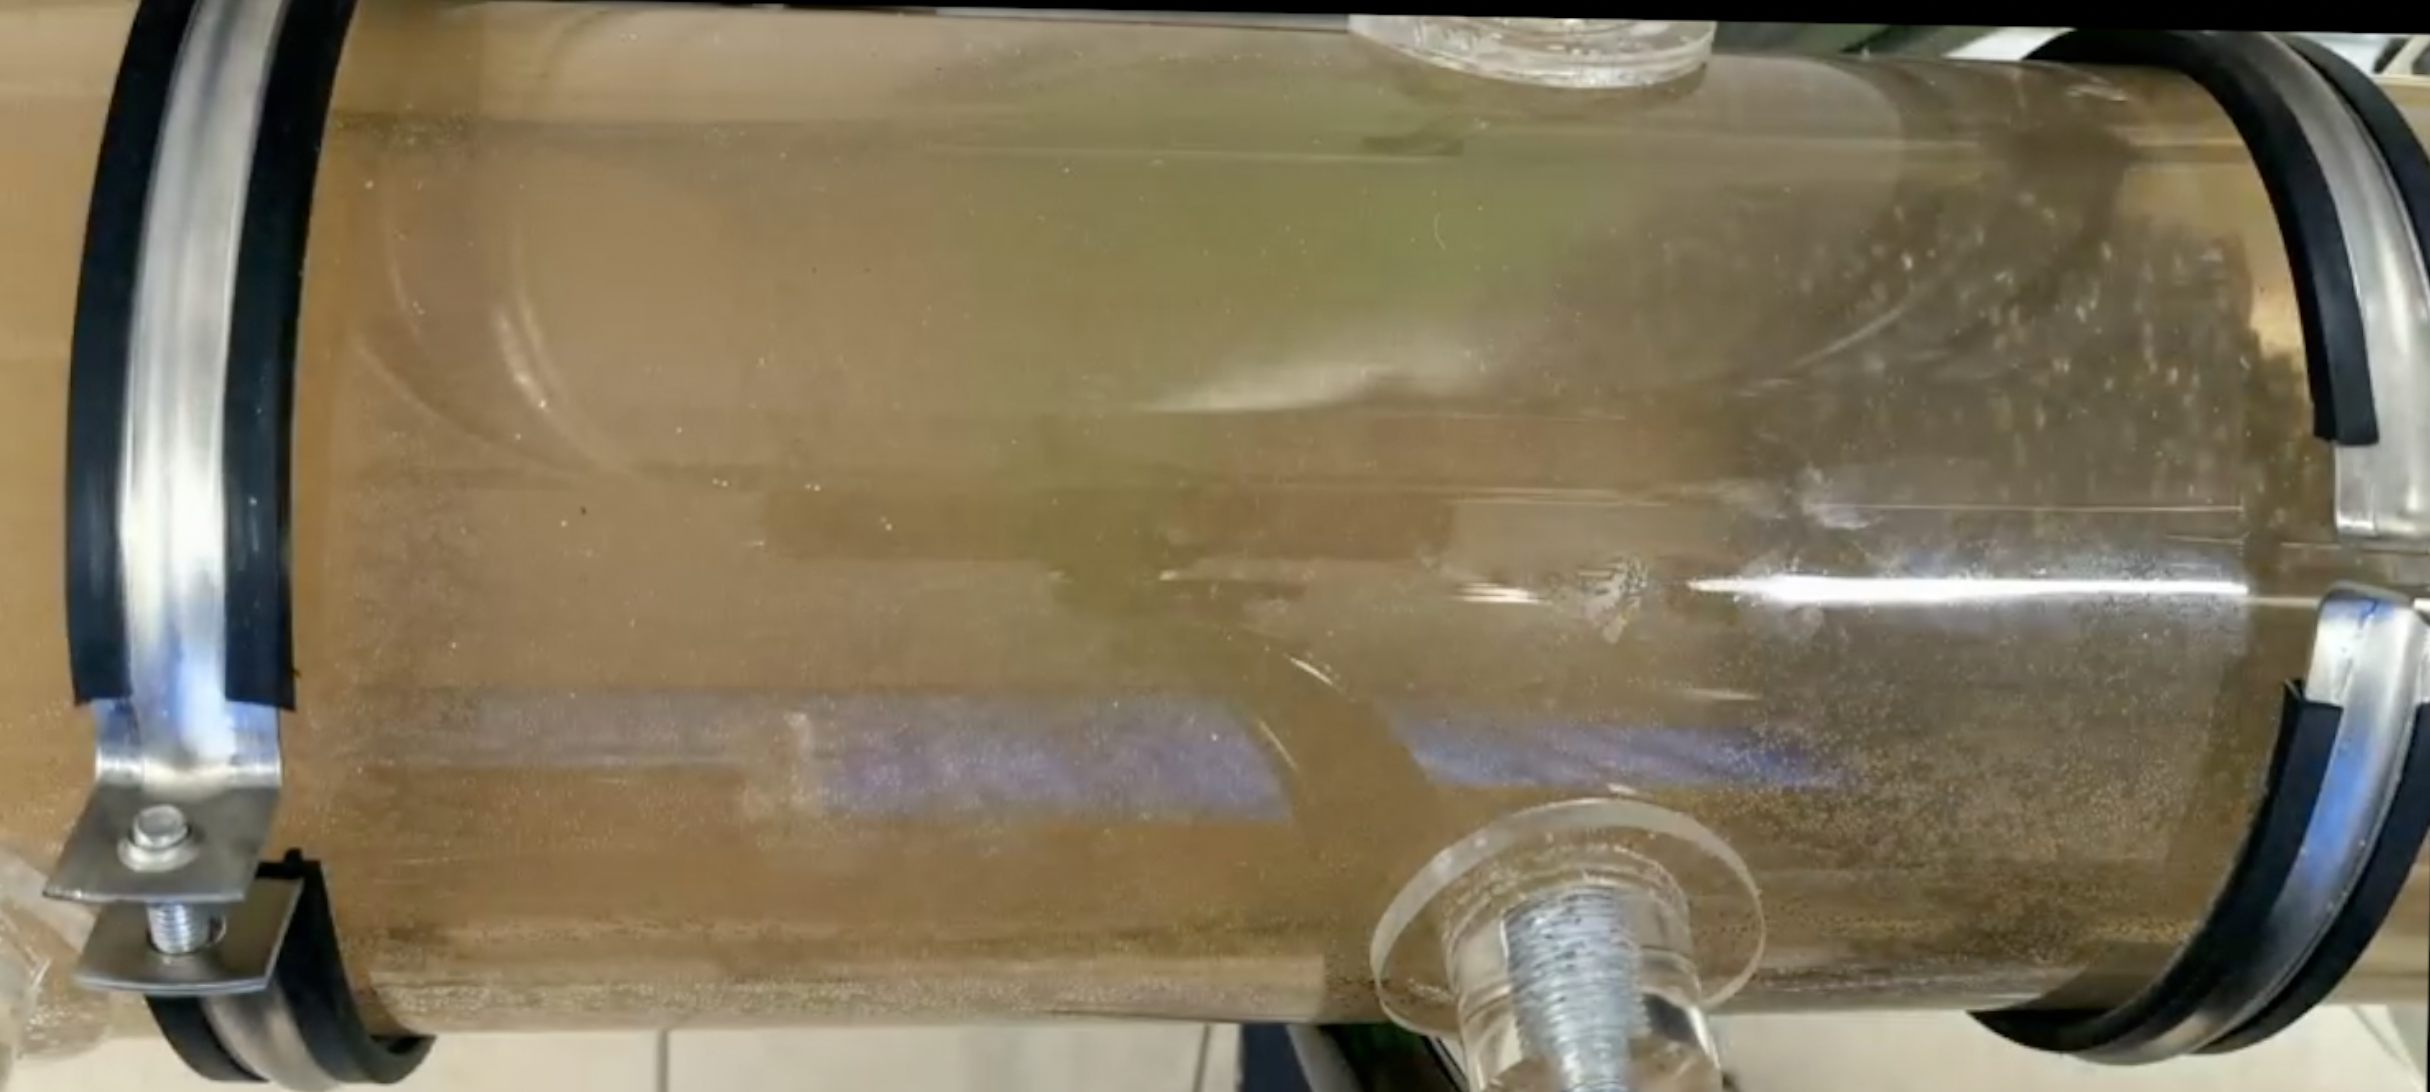
\includegraphics[width=.33\textwidth]{figure/chapter2/iron-bed-7dot85mperh.png}
	\label{fig:iron_bed_7dot85mperh}
	}
	%\vspace{1em}
	\subfloat[$Q=10.00\mathrm{m^3/h}$]{%
	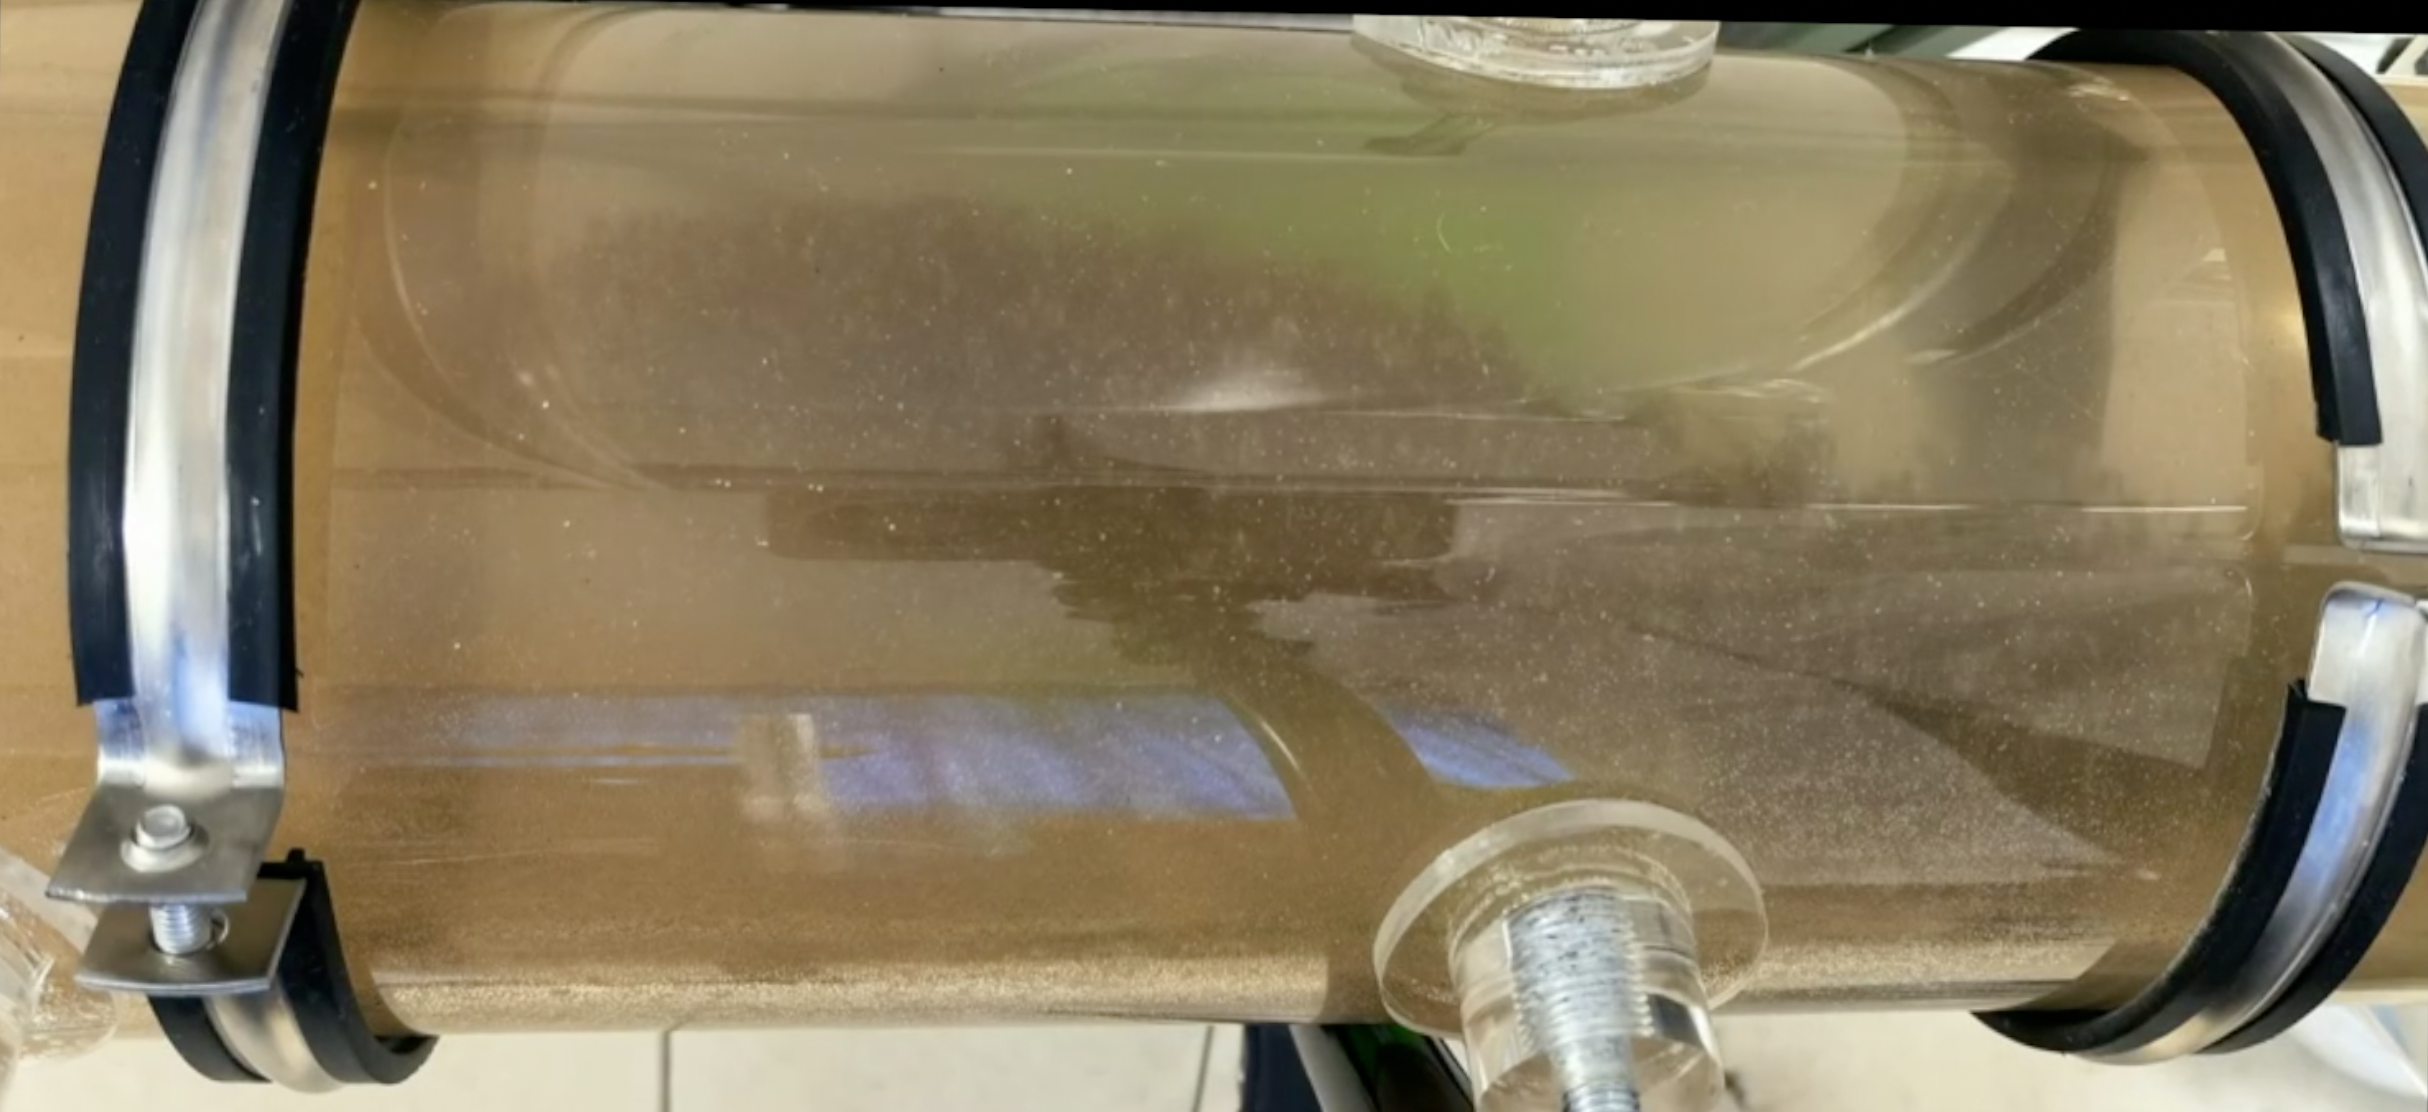
\includegraphics[width=.33\textwidth]{figure/chapter2/iron-bed-10dot00mperh.png}
	\label{fig:iron_bed_10dot00mperh}
	}
	\subfloat[$Q=11.70\mathrm{m^3/h}$]{%
	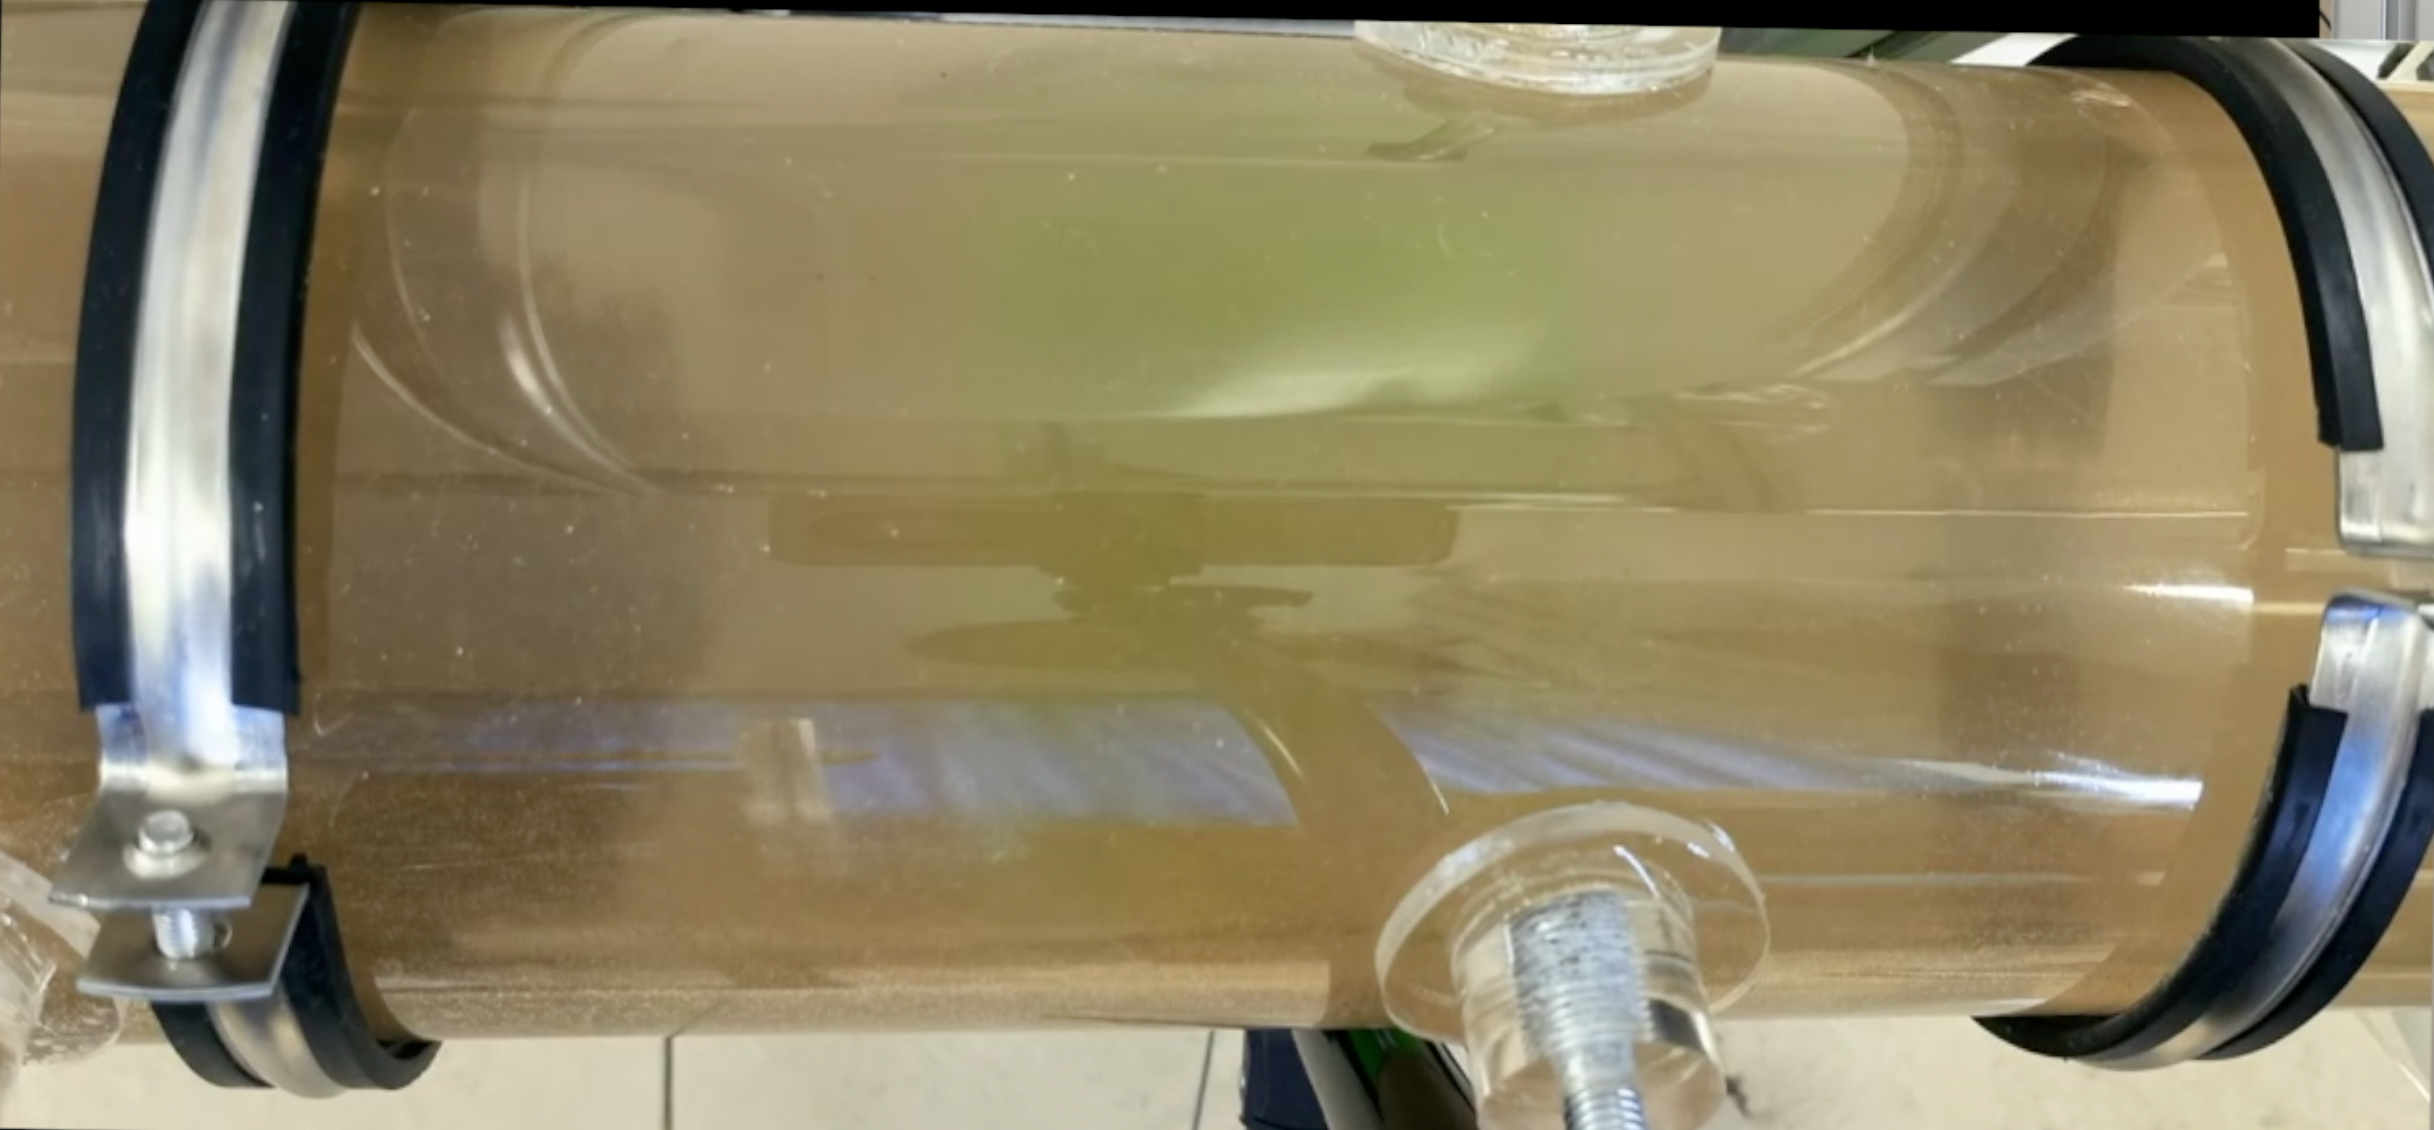
\includegraphics[width=.33\textwidth]{figure/chapter2/iron-bed-11dot70mperh.png}
	\label{fig:iron_bed_11dot70_mperh}
	}
	\caption{铁屑床初始形态（铁屑床初始位置处俯视相机拍摄）}
	\label{fig:initial_bed_profile}
\end{figure}

随着流量的逐级提升，铁屑床表现出复杂的运动特征。即便在水平管段，颗粒床在达到临界启动流量后也非呈现简单的整体滑移模式，而是表现出“前缘不断剥蚀消失、后缘持续重塑堆积”的动态演化规律，且在整个运移过程中都有部分细小碎屑会受流体曳力作用从床层主体剥离，随主流场输运，导致铁屑床的质量递减。床层整体的运移速度随流速的增加而提升，相对于环空的平均流速而言是较小值。

\begin{figure}[htbp]
	\centering
	\subfloat[$Q=15.70\mathrm{m^3/h}$]{%
	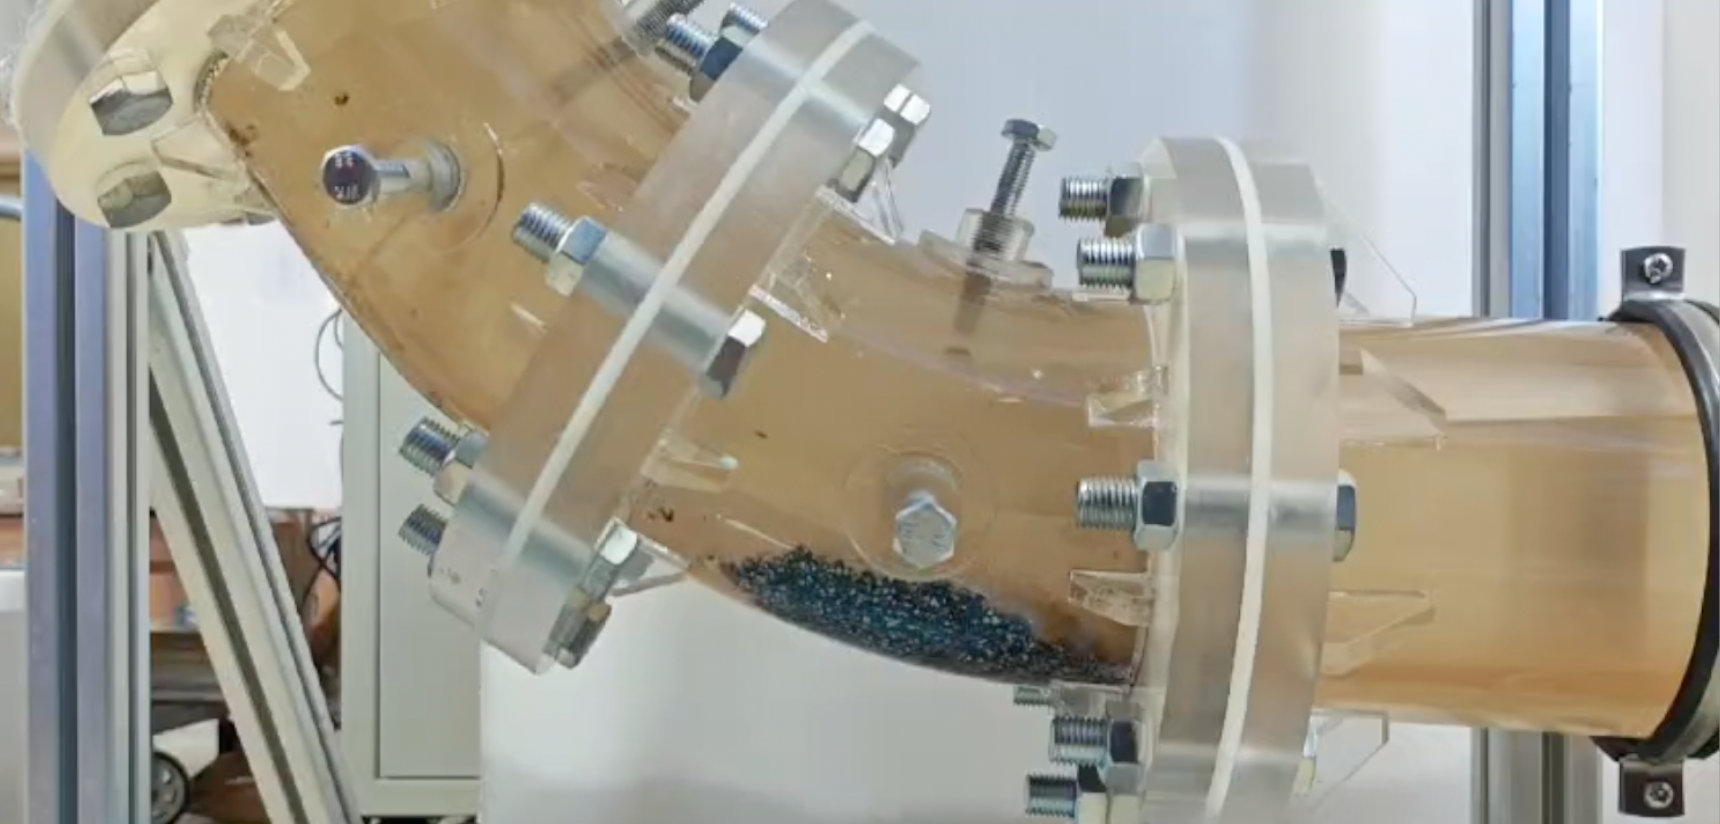
\includegraphics[width=.33\textwidth]{figure/chapter2/iron-bed-15dot70mperh.png}
	\label{fig:iron_bed_15dot70mperh}
	}
	%\vspace{1em}
	\subfloat[$Q=15.83\mathrm{m^3/h}$]{%
	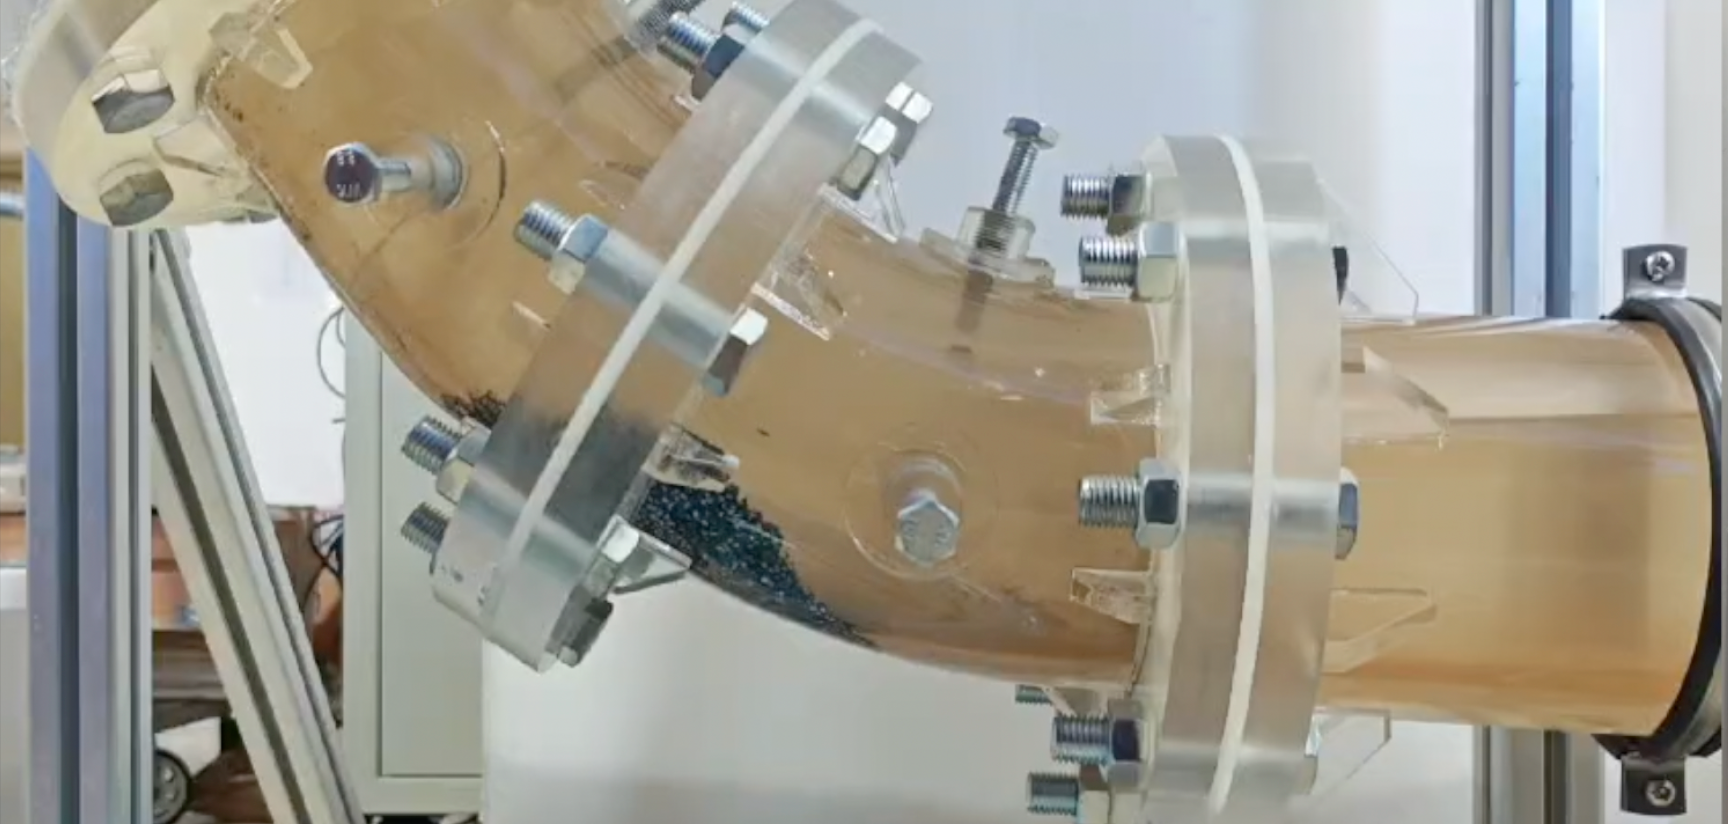
\includegraphics[width=.33\textwidth]{figure/chapter2/iron-bed-15dot83mperh.png}
	\label{fig:iron_bed_15dot83mperh}
	}
	\subfloat[$Q=17.44\mathrm{m^3/h}$]{%
	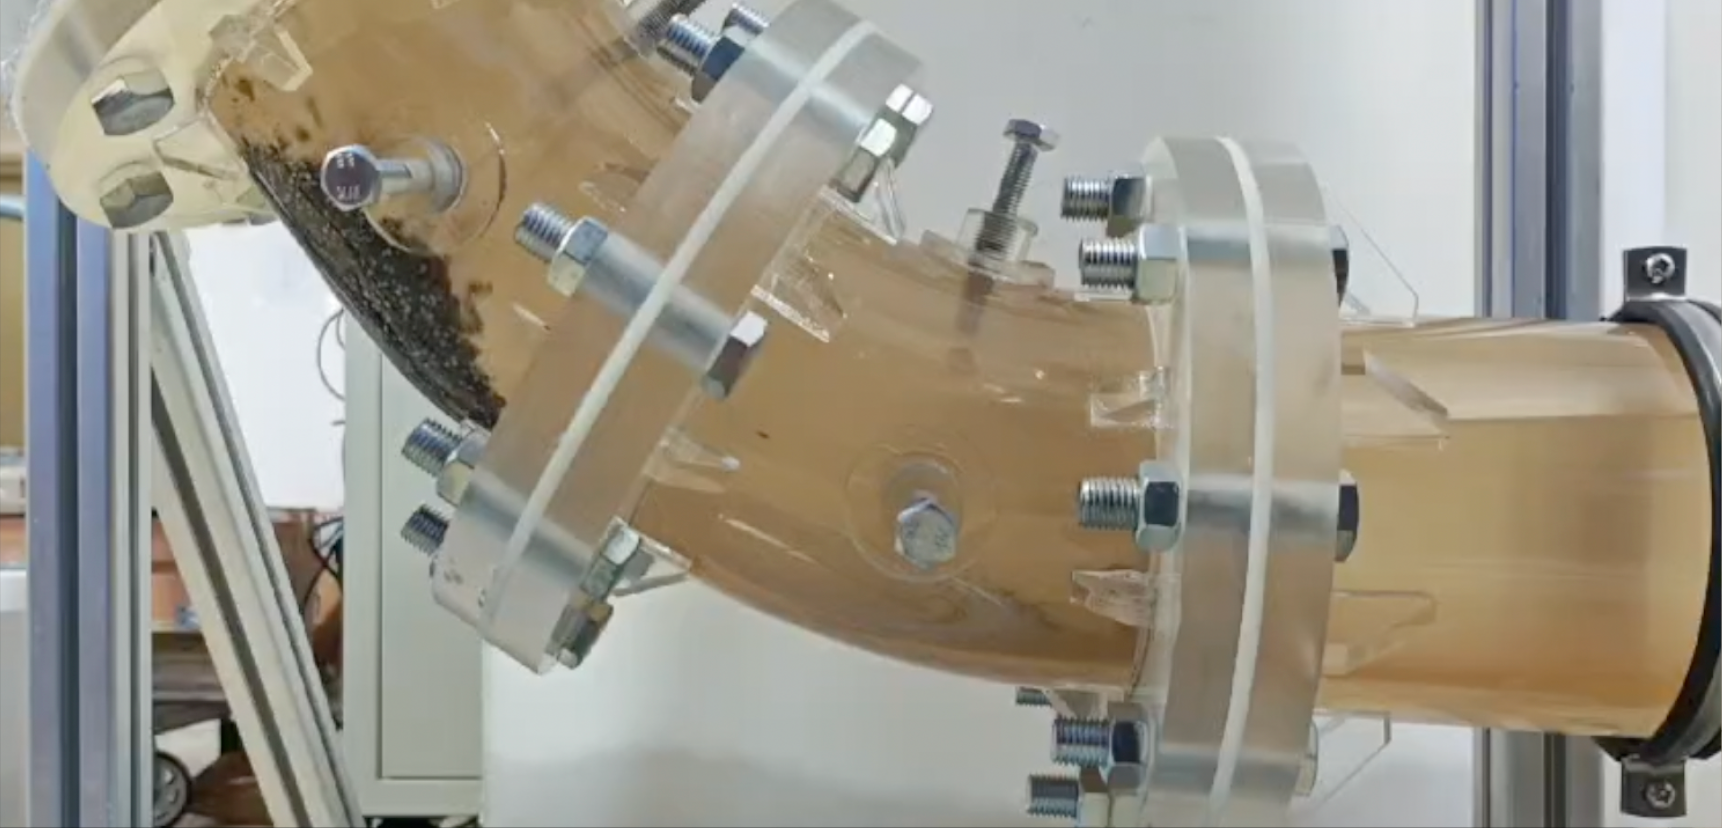
\includegraphics[width=.33\textwidth]{figure/chapter2/iron-bed-17dot44mperh.png}
	\label{fig:iron_bed_17dot44_mperh}
	}
	\caption{弯管段铁屑床形态（弯管处正视相机拍摄）}
	\label{fig:initial_bed_profile}
\end{figure}


\begin{figure}[htbp]
	\centering
	\subfloat[铁屑床形态视频截图]{%
	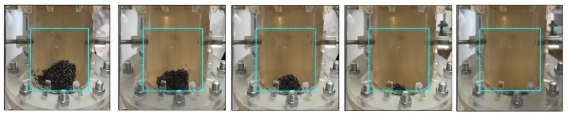
\includegraphics[width=.9\textwidth]{figure/chapter2/video-clip-theta-le-72-degree.png}
	\label{fig:video_clip_theta_le_72_degree}
	}
	\vspace{.5em}
	\subfloat[床面积提取结果]{%
	\begin{tikzpicture}
        % ================= 1. 放置完整的大图 =================
        % [name=img] 为图片命名，方便我们后续获取它的宽度
        % 替换 example-image 为你拼接好的那张完整大图的真实文件名（例如 full_image.png）
        \node[inner sep=0] (img) {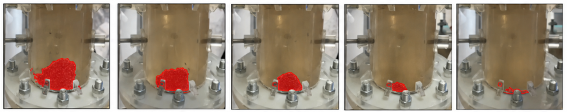
\includegraphics[width=.9\textwidth]{figure/chapter2/extraction-of-pack-area-theta-le-72-degree.png}};
        % ================= 2. 设置注释参数 =================
        % 这里的坐标是相对于大图的左下角 (0,0) 计算的
        \def\texty{-1.6} % 控制所有文字距离图片底部的垂直距离 (根据图片比例调整，负数表示向下偏移)
        % ================= 3. 在绝对坐标处添加注释 =================
        % 这里的 x 坐标（如 1.8, 3.6 等）是等间距的
        % 你需要根据你真实图片中子图的间距，手动微调这些 x 坐标
        \node at (-6.0, \texty) {${A^* = 1.00}$};
        \node at (-3., \texty) {${A^* = 0.64}$};
        \node at (0.0, \texty) {${A^* = 0.34}$};
        \node at (3., \texty) {${A^* = 0.05}$};
        \node at (6., \texty) {${A^* \approx 0.00}$};
    \end{tikzpicture}
	\label{fig:extraction_of_pack_area_theta_le_72_degree}
	}
	\caption{竖直段铁屑床形态（竖直管左视相机拍摄）}
	\label{fig:initial_bed_profile}
\end{figure}

为精确量化这一过程，实验后期通过视频帧分析提取了关键时间节点下的流量、位置及残留状态数据；特别是在弯管段的位置标定中，采用了实验视频与带刻度三维模型重叠匹配的方法，通过读取铁屑堆首尾端的刻度值，精确解算了床层质心的空间位置。实验观测表明，铁屑在弯管内的宏观迁移与进入竖直段后的流态化消散呈现出截然不同的动力学特征。前者主要体现为床层整体位置的时空演变，后者则侧重于固定堆积量的衰减过程。鉴于此，后续数据处理将针对这两个阶段分别选取特定的响应变量进行定量分析。

位置标定数据来自对原始视频的逐帧标定：在每个时刻识别铁屑床的头部与尾部，取二者角度的平均值作为床层中部位置，并记录对应的流量读数。标定共获得 $20$ 个有效点，角度范围覆盖 $\theta_c=0^{\circ}$-$72^{\circ}$，流量 $Q=14.25$-$18.09 \mathrm{m^3/h}$。其中 $\theta_c=51^{\circ}$-$63^{\circ}$区间因流量计读数在该时间段内出现异常波动，原始记录未采集到有效数据，这一区间在后续拟合中不参与计算，模型曲线由两侧的数据共同约束、连续给出。
$\theta_c>72^{\circ}$后，铁屑床主要进入竖直观察段并局部堆积，用弯管角度描述位置已不再适用，因此第二阶段改用视频提取的固定床可见面积作为响应量，用以描述床层的消散过程。

在弯管迁移阶段，驱动铁屑床向前移动的是水流对床层的作用力，而阻碍其移动的主要是重力沿弯管切线方向的分量。参考直管水力学中过流量与壁面切应力的关系，流体作用力近似随流量的平方（$Q^2$）增长；重力切向分量则随弯管角度的正弦（$\sin\theta_c$）增长，在 $\theta_c^\circ$ 处最小、随角度增大而增大。将两者放在同一个力平衡框架下，可以得到如下候选形式
\begin{equation}
	Q^2(\theta) = A + B\cdot \sin\theta
\end{equation}
式中，$A$、$B$为待定系数，量纲均为 $\mathrm{(m^3/h)^2}$。这一形式只用到了两个可从数据中辨识的组合参数，物理方向与力平衡机制一致，是后续候选模型比较的核心对象。

为避免主观选定单一形式，本文在同一数据集上比较了四类候选模型（见表\ref{tab:model_comparison}），统一以流量$Q$作为响应变量，通过决定系数$R^2$、均方根误差 RMSE、修正后的 AICc 以及留一交叉验证 RMSE（LOOCV RMSE）综合评估拟合优度与泛化能力：

\begin{table}[htbp]
    \centering
    \caption{候选模型拟合与交叉验证结果对比}
    \label{tab:model_comparison}
    \renewcommand{\arraystretch}{1.3}
    \begin{tabular}{llccccc}
        \toprule
        模型 & 函数形式 & 参数个数 & $R^2$ & RMSE & AICc & LOOCV RMSE \\
        \midrule
        重力分量力平衡 & $Q^2 = A + B\sin\theta_c$ & 2 & 0.942 & 0.267 & -48.15 & 0.294 \\
        二次多项式 & $Q = a + b\theta + c\theta_c^2$ & 3 & 0.943 & 0.265 & -45.63 & 0.302 \\
        经验幂函数 & $Q = Q_0 + c\theta_c^p$ & 3 & 0.945 & 0.261 & -46.26 & 0.313 \\
        线性 & $Q = a + b\theta_c$ & 2 & 0.911 & 0.331 & -39.50 & 0.376 \\
        \bottomrule
    \end{tabular}
\end{table}

二次多项式与经验幂函数的样本内 $R^2$ 略高于力平衡模型，但二者多用了一个自由参数，留一交叉验证误差反而没有改善，说明额外的自由度更多是在拟合噪声而非提升泛化能力。重力分量力平衡模型同时取得最低的 AICc 和最低的 LOOCV RMSE，且只用两个参数即达到与三参数模型相当的拟合优度，因此被选为最终模型。更高阶的分段拟合虽然可能进一步推高样本内 $R^2$ ，但会把 $\theta_c=51^\circ$～$63^\circ$ 的数据缺失和流量的局部波动误拟合成结构性拐点，不适合当前的数据规模。基于 $20$个有效位置点，最终确定的弯管迁移阶段模型为
\begin{equation}
	Q^2(\theta_c) = 208.57 + 122.69\sin \theta_c,  0^\circ \le \theta_c \le 72^\circ
\end{equation}
其中，基线项 $208.57$ 代表弯管起点附近床层接触、形状嵌锁与摩擦等综合阻力所对应的启动流量平方；系数 $122.69$ 代表重力切向分量随角度上升而增加的贡献。模型整体 $R^2$为 $0.942$，流量 RMSE 为 $0.267 \mathrm{m^3/h}$，LOOCV RMSE 为 $0.294 \mathrm{m^3/h}$。参数的 Bootstrap 95\% 置信区间为 $A \in [202.43, 216.75]$，$B \in [107.72, 134.89]$。由基线项换算得到的模型基准启动流量为 $Q_0 = 14.44 \mathrm{m^3/h}$（95\% 区间 $14.23-14.72 \mathrm{m^3/h}$），与实测中铁屑床到达弯管起始处的流量$14.25\mathrm{m^3/h}$ 十分接近，二者相互印证，说明模型在起点附近具有良好的物理合理性。

现有材料足以建立“弯管迁移 + 竖直段衰减”的两阶段半经验模型，并可靠给出本装置的一次实验启动、迁移和完全冲洗区间；但不足以识别可外推到其他管径、液体或铁屑形态的完整Exner模型、Shields临界模型或两层流模型。


最终实验表明，随着泵流量增加，铁屑床经历由启动、沿弯管迁移、进入竖直段聚集并逐渐衰减，直至无可见颗粒的连续变化过程。约21.5m³/h可作为本次实验条件下的最小观察性完全冲洗参考流量，而约21.8m³/h可作为本台架复现实验中较保守的无可见颗粒确认流量。
上述结论来源于本装置、本次约70g短小卷曲车削铁屑以及当前流体条件下的一次连续升流量实验。由于流量与时间在本次试验中同步变化，且缺少多组恒定流量下的重复试验，因此所得模型和特征流量主要用于描述本台架条件下的实验规律，不宜直接外推至其他管径、其他铁屑形态或现场工况。

 % 全井筒模型
% --- 第三章 ---
%\chapter{深度清洁工具设计}

%井筒清洁是油气井作业的关键工序，其核心是清除井筒内的岩屑、砂粒、蜡垢、水垢、腐蚀产物等杂质，以保障井筒畅通、恢复产能、延长服役寿命，贯穿钻井、完井、修井及生产的全周期。现有井筒清洁技术功能单一、施工效率低，一体化与集成化程度低，难以满足油田开采降本增效的需求。为此，本研究通过理论研究丰富产品系列，形成了一套针对 9-5/8\inch 井筒的深度清洁工艺技术。本章针对该工艺技术的核心清洁工具，按照单工具工艺与工具组合工艺两部分展开：首先分别完成“三合一”脉冲式冲刮刷集成式井筒清洁工具、“四合一”通刮刷磁集成式井筒清洁工具、大容量强磁吸附工具、多功能过滤工具和可变径刮管工具的结构设计、理论计算与仿真校核，并给出各工具的使用与维护要求；然后结合不同井况要求给出上述工具的组合方式，以减少下钻趟数、提高作业效率。

\chapter[“三合一”脉冲式冲刮刷集成式井筒清洁工具设计]{“三合一”脉冲式冲刮刷集成式井筒清洁工具设计\protect\footnote{合同条款：5.1.3井筒高效清洁关键技术配套工具设计——（5）“三合一”脉冲式冲刮刷集成式井筒清洁工具设计}}\label{sec:design_of_3_in_1}
	实验表明，对于连续砂床或严重出砂井况，常规水力冲砂冲砂效率低，除砂效果差。针对此难题，本章主要开展水力脉冲冲砂洗井工具结构设计并阐述冲砂洗井工具的结构组成和工作原理，然后建立水力脉冲脉冲洗井工具数学模型并通过CFD仿真验证工具的冲砂效果。

\subsection{水力脉冲冲砂洗井工具结构组成}

水力脉冲冲砂洗井工具主要由脉冲发生模块与旋转喷头模块构成,如图\ref{fig:tool_structure_3_in_1}所示。旋转喷头模块的核心功能在于利用前向布置的高压喷嘴产生强力射流，直接作用于井底沉积砂床，通过流体的高剪切应力实现对砂床表面的破坏与砂砾的卷扬，使沉积颗粒在卷扬作用下重新进入悬浮运移状态；同时，配合周向旋转机构实现的 全覆盖喷射，消除了常规清洗中的水力死角。脉冲模块则负责产生一种具有低频特性的高、负压交替水力冲击波。该模块通过对油套管内壁进行高频次的反复激励，利用压力脉动产生的振动效应有效疏通并剥离附着于管壁的坚硬垢层与残留杂质。更为关键的是，水力冲击波在环空流体中传播时，能为已沉积或趋于沉积的砂砾提供额外的扰动动能，破坏颗粒间的动力平衡状态，从而显著提升井筒清砂的整体作业效率。

\begin{figure}[htbp]
	\centering
	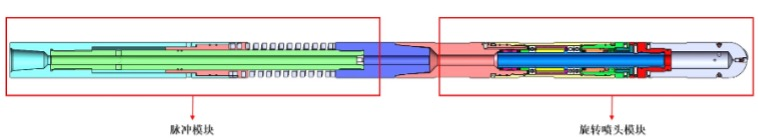
\includegraphics[width=1.\textwidth]{figure/chapter3/tool-structure-3-in-1.jpg}
	\caption{水力脉冲冲砂洗井工具结构示意图}
	\label{fig:tool_structure_3_in_1}
\end{figure}

\subsection{水力脉冲冲砂洗井工具结构设计及工作原理}

\subsubsection{水力脉冲冲砂洗井工具旋转喷头模块设计}
如图\ref{fig:nozzle_sub}所示，旋转喷头模块主要由上接头、筒体、芯轴、连通隔套、平衡活塞、底部帽、平衡活塞座、喷头连接体、隔套、座、旋转喷头、喷嘴和骨架油封等密封件以及轴承和复位弹簧等零部件组成。其工作原理是旋转喷头模块位于工具作业串的最前端，用钻杆送入至指定的位置，其余工具固定好之后，开泵循环泵入介质，流体由工具上接头导入，沿中心芯轴流道行进，最终经由端部喷嘴高速喷出。在此输运过程中，由于工具内部流道截面积缩小，流体节流从而产生巨大压降，流速增快从而产生冲击效果。此外，为实现全向清洗，喷头结构中设计了两组具有特定偏心夹角的喷嘴。当高速介质经由倾斜流道射出时，射流产生的反冲推力在工具横截面上形成持续的偏心力矩，该力矩直接驱动旋转喷头与芯轴自转，进而实现对套管内壁 360° 无死角的周向清洗。

\begin{figure}[htbp]
	\centering
	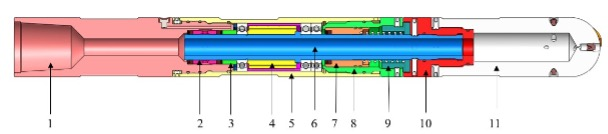
\includegraphics[width=1.0\textwidth]{figure/chapter3/nozzle-sub.jpg}
	\caption{水力脉冲冲砂洗井工具结构示意图}
	\label{fig:nozzle_sub}
\end{figure}

\subsubsection{水力脉冲冲砂洗井工具脉冲发生模块设计}

如图\ref{fig:pulse_module}所示，脉冲发生模块由上接头、芯轴、移动活塞、矩形弹簧、下接头组成。其工作原理是脉冲发生模块圆周上设计有出水孔，靠地面泵或注水管线，把液体传入井下，水流通过节流喷嘴时会产生节流压差，对脉冲器活塞面产生高压作用。

\begin{figure}[htbp]
	\centering
	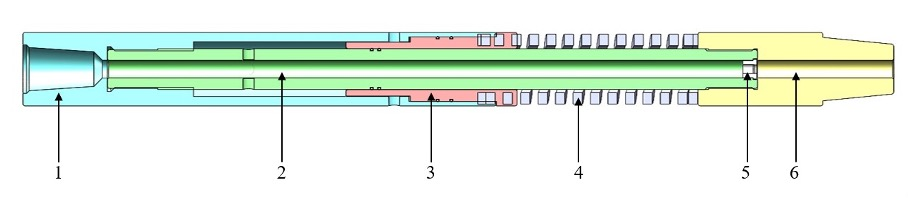
\includegraphics[width=1.0\textwidth]{figure/chapter3/pulse-module.jpg}
	\caption{水力脉冲冲砂洗井工具脉冲发生模块结构图}
	\label{fig:pulse_module}
\end{figure}


脉冲发生模块的工作原理如\ref{fig:principle_of_pulsing_tool}所示。在高压作用下，活塞克服矩形弹簧的预紧力及流体的粘滞及摩擦阻力产生轴向位移，当活塞上端面到达侧向出水孔时，侧向出水孔开启，高压水射流从侧向出水孔喷出，腔内压力开始下降，活塞在弹簧压缩力的作用下开始复位，侧向出水孔关闭。活塞复位到初始位置，系统开始下一循环。

该装置向井筒环空传递振动能量的途径主要包括两种机制：首先是振动器本体产生的轴向机械振荡；其次是由高压脉冲流体激发的径向水力冲击效应。在上述复合动载荷的共同叠加下，环空内的局部流场呈现出强烈的瞬态扰动特性。原本压实沉积的砂床结构被脉冲射流破坏，砂粒由静态沉降转变为悬浮流化状态，进而配合循环工作液被高效排出井筒。

\begin{figure}[htbp]
	\centering
	\subfloat[脉冲发生模块蓄能阶段]{%
	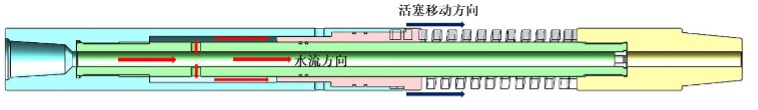
\includegraphics[width=0.9\textwidth]{figure/chapter3/energy-storage-in-pulse-module.jpg}
	}
	\vspace{1em}
	\subfloat[脉冲发生模块复位阶段]{%
	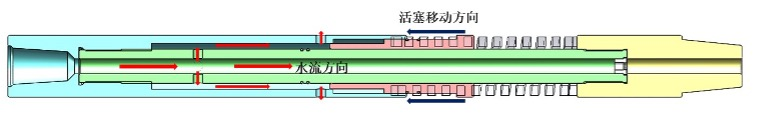
\includegraphics[width=0.9\textwidth]{figure/chapter3/restore-in-pulse-module.jpg}
	}
	\caption{脉冲发生器工作原理}
	\label{fig:principle_of_pulsing_tool}
\end{figure}

\subsubsection{毛刷刮管模块设计}

MSQ型毛刷刮管器是用于清除井下套管内壁上的残余水泥，泥块、生产井套管上的铁锈，水垢，硬石蜡等影响正常施工作业杂物的工具。MSQ型毛刷刮管器主要由上接头、上扶正套、毛刷体、下扶正套、剪切套、剪切定位套、下接头等部件组成。其工作时主要靠上毛刷和下毛刷对刮削过的套管内壁进行刷洗清洁。在浅井内工作时主要靠下毛刷对套管内壁进行刷洗清洁，当刮削到一定深度后，下毛刷发生磨损后上毛刷体可自动伸出参与刷洗清洁，从而保证在整个作业过程中套管清洁的质量。

\begin{figure}[htbp]
	\centering
	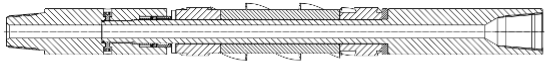
\includegraphics[width=0.9\textwidth]{figure/chapter3/swiper-in-3-in-1.png}
	\caption{毛刷刮管器结构简图}
	\label{fig:swiper_in_3_in_1}
\end{figure}

工具的技术参数如下表所示。


\begin{table}[htbp]
    \centering
    \caption{脉冲器技术参数}
    \label{tab:pulsar_params}
    \renewcommand{\arraystretch}{1.5} % 增加行高，使表格更美观
    \begin{tabularx}{1.\textwidth}{cXcccccc}
        \toprule % 顶线
        代号 & 适用套管规格 & \begin{tabular}[c]{@{}c@{}}组装外径\\ (mm)\end{tabular} & \begin{tabular}[c]{@{}c@{}}最小通径\\ (mm)\end{tabular} & \begin{tabular}[c]{@{}c@{}}长度\\ (mm)\end{tabular} & \begin{tabular}[c]{@{}c@{}}最大抗拉\\ (kN)\end{tabular} & \begin{tabular}[c]{@{}c@{}}最大抗扭\\ ($\text{kN}\cdot\text{m}$)\end{tabular} & 连接螺纹 \\
        \midrule % 栏目线
        MSQ105 & $4-1/2''$ & 105 & 25 & 1250 & 912 & 14.2 & \begin{tabular}[c]{@{}c@{}}NC31\\ ($\text{P}\times\text{B}$)\end{tabular} \\
        \bottomrule % 底线
    \end{tabularx}
\end{table}

\begin{table}[htbp]
    \centering
    \caption{旋转喷头技术参数}
    \label{tab:rotary_nozzle_params}
    \renewcommand{\arraystretch}{1.5} % 增加行高，使表格更美观
    \begin{tabularx}{1.\textwidth}{ccccccccc}
        \toprule % 顶线
        \begin{tabular}[c]{@{}c@{}}外径\\ (mm)\end{tabular} & 
        \begin{tabular}[c]{@{}c@{}}总长\\ (mm)\end{tabular} & 
        \begin{tabular}[c]{@{}c@{}}喷嘴尺寸\\ （mm $\times$ n）\end{tabular} & 
        \begin{tabular}[c]{@{}c@{}}工作排量\\ (L/min)\end{tabular} & 
        \begin{tabular}[c]{@{}c@{}}转速\\ (r/min)\end{tabular} & 
        \begin{tabular}[c]{@{}c@{}}工作压强\\ (MPa)\end{tabular} & 
        扣型 & 
        \begin{tabular}[c]{@{}c@{}}最大抗拉\\ (kN)\end{tabular} & 
        \begin{tabular}[c]{@{}c@{}}最大抗扭\\ ($\text{kN}\cdot\text{m}$)\end{tabular} \\
        \midrule % 栏目线
        105 & 1045 & $3.175 \times 7$ & 100-500 & 10-300 & $\le 70$ & \begin{tabular}[c]{@{}c@{}}NC31\\ ($\text{P}\times\text{B}$)\end{tabular} & 663 & 8.5 \\
        \bottomrule % 底线
    \end{tabularx}
\end{table}


\begin{table}[htbp]
    \centering
    \caption{液压刮管器技术参数}
    \label{tab:hydraulic_scraper_params}
    \renewcommand{\arraystretch}{1.5} % 增加行高，使表格更美观
    \begin{tabularx}{1.\textwidth}{ccXcccc}
        \toprule % 顶线
        代号 & 适用套管规格 & \begin{tabular}[c]{@{}c@{}}组装外径\\ (mm)\end{tabular} & \begin{tabular}[c]{@{}c@{}}最小通径\\ (mm)\end{tabular} & \begin{tabular}[c]{@{}c@{}}投入钢球\\ (mm)\end{tabular} & \begin{tabular}[c]{@{}c@{}}张开直径\\ (mm)\end{tabular} & 连接螺纹 \\
        \midrule % 栏目线
        YYGG105 & $4-1/2''$ & 114 & 22 & 30/35 & 130 & NC31($\text{P}\times\text{B}$) \\
        \bottomrule % 底线
    \end{tabularx}
\end{table}

\begin{table}[htbp]
    \centering
    \caption{毛刷刮管器技术参数}
    \label{tab:brush_scraper_params}
    \renewcommand{\arraystretch}{1.5} % 增加行高，使表格更美观
    \begin{tabularx}{1.\textwidth}{ccXccc}
        \toprule % 顶线
        型号 & 
        \begin{tabular}[c]{@{}c@{}}最大外径\\ (mm)\end{tabular} & 
        \begin{tabular}[c]{@{}c@{}}毛刷最大外径\\ (mm)\end{tabular} & 
        \begin{tabular}[c]{@{}c@{}}水眼\\ (mm)\end{tabular} & 
        \begin{tabular}[c]{@{}c@{}}总长\\ (mm)\end{tabular} & 
        接头扣 \\
        \midrule % 栏目线
        MSQ54 & 105 & 130 & 20 & 1250 & NC31($\text{P}\times\text{B}$) \\
        \bottomrule % 底线
    \end{tabularx}
\end{table}


\subsection{设计计算与校核}

\subsubsection{脉冲器计算与校核}

脉冲器设计要求如下表所示。

\begin{table}[htbp]
    \centering
    \caption{脉冲器设计要求}
    \label{tab:pulsar_design_req}
    \renewcommand{\arraystretch}{1.5} % 增加行高，使表格更美观
    \begin{tabularx}{1.\textwidth}{Xccccc}
        \toprule % 顶线
        \begin{tabular}[c]{@{}c@{}}外径\\ (mm)\end{tabular} & 
        \begin{tabular}[c]{@{}c@{}}水眼直径\\ (mm)\end{tabular} & 
        接头螺纹扣型 & 
        \begin{tabular}[c]{@{}c@{}}许用拉力\\ (kN)\end{tabular} & 
        \begin{tabular}[c]{@{}c@{}}许用扭矩\\ ($\text{kN}\cdot\text{m}$)\end{tabular} & 
        \begin{tabular}[c]{@{}c@{}}总长\\ (mm)\end{tabular} \\
        \midrule % 栏目线
        105 & 25 & NC31 & 400 & 8 & 1250 \\
        \bottomrule % 底线
    \end{tabularx}
\end{table}


该产品为井下清洁工具，所以它的工作条件十分恶劣。根据产品的结构，它属于中间空的细长杆件且筒体较薄类型。依API标准对钻具的材料要求，选取具有较高强度的4145H合金结构钢并经调质处理，作为产品的主体结构材料。钢材的成份应符合ASTM A304-05e2标准的规定。
为了适应工作条件下的应力状态，热处理后的力学性能应达到以下要求。

\begin{table}[htbp]
    \centering
    \caption{产品要求}
    \label{tab:product_requirements}
    \renewcommand{\arraystretch}{1.5} % 增加行高，使表格更美观
    \begin{tabularx}{1.\textwidth}{cXcc}
        \toprule % 顶线
        硬度 & 最小屈服强度 & 伸长率 & 夏比冲击功 \\
        \midrule % 栏目线
        285-321(HB) & $\sigma_S \ge 785\text{MPa}$ & $13\%$ & $Akv \ge 54\text{J}$ \\
        \bottomrule % 底线
    \end{tabularx}
\end{table}


1） 危险截面（螺纹应力分散槽处）抗拉抗扭计算

（1）许用拉力计算

\begin{equation}
    F_{\max} = \frac{[\pi \cdot (D^2 - d^2)] \cdot \sigma_s}{4 \cdot n} \times 10^{-3}
\end{equation}
式中，$F_{\max}$ — 工具最大拉力，kN；

$D$ — 危险截面外径，mm；

$d$ — 危险截面内径，mm；

$\sigma_s$ — 材料最小屈服强度：825 MPa (4145H)；

$n$ — 安全系数，取 $n = 1.5$。

代入数据计算如下：
\begin{align}
    F_{\max} &= \frac{\pi \cdot (D^2 - d^2) \cdot \sigma_s}{4 \cdot n} \times 10^{-3} \\
             &= \frac{3.14 \times (50^2 - 30^2) \times 825}{4 \times 1.5} \times 10^{-3} \\
             &= 690.8 \, \text{kN} \\
             &> 400 \, \text{kN}
\end{align}
满足设计要求。

(2) 许用扭矩计算

\begin{equation}
    T_{\max} = \frac{\sigma_s \cdot \pi \cdot (D^4 - d^4)}{16 \cdot D \cdot n} \times 10^{-6}
\end{equation}
式中，$T_{\max}$ — 最大扭矩，$\text{kN} \cdot \text{m}$；

$\sigma_s$ — 材料屈服应力，MPa；

$D$ — 危险截面外径，mm；

$d$ — 危险截面内径，mm；

$n$ — 安全系数，根据《机械设计手册》，取 $n = 1.5$。

代入数据计算得
\begin{align}
    T_{\max} &= \frac{\sigma_s \cdot \pi \cdot (D^4 - d^4)}{16 \cdot D \cdot n} \times 10^{-6} \\
             &= \frac{825 \times 3.14 \times (50^4 - 30^4)}{16 \times 50 \times 1.5} \times 10^{-6} \\
             &= 11.74 \, \text{kN} \cdot \text{m} \\
             &> 8 \, \text{kN} \cdot \text{m}
\end{align}
满足设计要求。

2）主要受力件仿真校核

脉冲器的主要受力件为脉冲器心轴，危险截面出现在出水口，脉冲器芯轴的最大拉应力为630Mpa，小于设计要求，最大切应力为994Mpa，但范围极小，属于应力集中导致的局部小尺度高应力，不会引发整体塑性变形；强度满足设计要求。


\begin{figure}[htbp]
	\centering
	\subfloat[脉冲器心轴]{%
	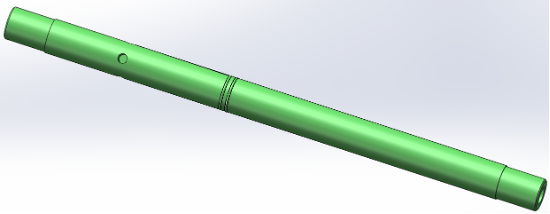
\includegraphics[width=0.7\textwidth]{figure/chapter3/inner-pipe-3-in-1.png}
	}
	\hfill
	\subfloat[抗拉强度分析]{%
	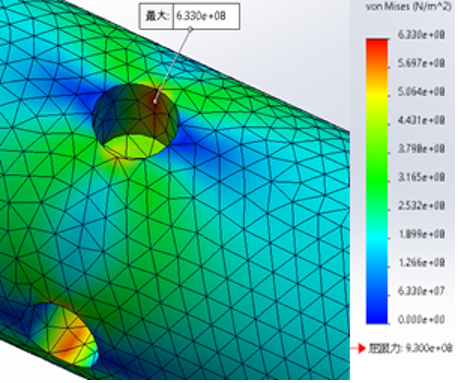
\includegraphics[width=0.4\textwidth]{figure/chapter3/inner-pipe-3-in-1-tensile-stress.png}
	}
	\vspace{1em}
	\subfloat[抗扭强度分析]{%
	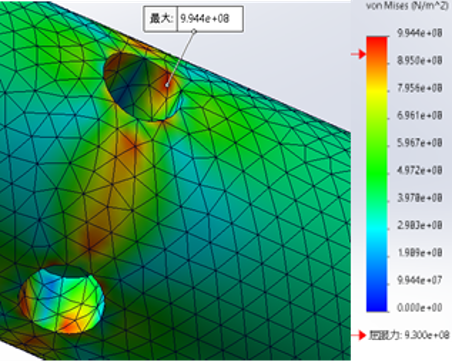
\includegraphics[width=0.45\textwidth]{figure/chapter3/inner-pipe-3-in-1-torsional-stress.png}
	}
	\caption{脉冲发生器薄弱零件强度有限元分析}
	\label{fig:FEA_inner_pipe_3_in_1}
\end{figure}
	% !TeX root = ../../main.tex
\section{设计计算与校核}

\subsection{脉冲器计算与校核}

脉冲器设计要求如下表所示。

\begin{table}[htbp]
    \centering
    \caption{脉冲器设计要求}
    \label{tab:pulsar_design_req}
    \renewcommand{\arraystretch}{1.5} % 增加行高，使表格更美观
    \begin{tabularx}{1.0\textwidth}{ccXccc}
        \toprule % 顶线
        \begin{tabular}[c]{@{}c@{}}外径\\ (mm)\end{tabular} & 
        \begin{tabular}[c]{@{}c@{}}水眼直径\\ (mm)\end{tabular} & 
        接头螺纹扣型 & 
        \begin{tabular}[c]{@{}c@{}}许用拉力\\ (kN)\end{tabular} & 
        \begin{tabular}[c]{@{}c@{}}许用扭矩\\ ($\text{kN}\cdot\text{m}$)\end{tabular} & 
        \begin{tabular}[c]{@{}c@{}}总长\\ (mm)\end{tabular} \\
        \midrule % 栏目线
        105 & 25 & NC31 & 400 & 8 & 1250 \\
        \bottomrule % 底线
    \end{tabularx}
\end{table}


该产品为井下清洁工具，工作条件十分恶劣，其结构属于中间空的细长杆件且筒体较薄。依据API标准对钻具的材料要求，选用具有较高强度的4145H合金结构钢并经调质处理，作为产品的主体结构材料，钢材成分应符合ASTM A304-05e2标准的规定。
为适应工作条件下的应力状态，热处理后的力学性能应达到以下要求。

\begin{table}[htbp]
    \centering
    \caption{产品要求}
    \label{tab:product_requirements}
    \renewcommand{\arraystretch}{1.5} % 增加行高，使表格更美观
    \begin{tabularx}{1.0\textwidth}{cXcc}
        \toprule % 顶线
        硬度 & 最小屈服强度 & 伸长率 & 夏比冲击功 \\
        \midrule % 栏目线
        285-321(HB) & $\sigma_S \ge 785\text{MPa}$ & $13\%$ & $Akv \ge 54\text{J}$ \\
        \bottomrule % 底线
    \end{tabularx}
\end{table}


1） 危险截面（螺纹应力分散槽处）抗拉抗扭计算

（1）许用拉力计算

\begin{equation}
    F_{\max} = \frac{[\pi \cdot (D^2 - d^2)] \cdot \sigma_s}{4 \cdot n} \times 10^{-3}
\end{equation}
式中，$F_{\max}$为工具最大拉力，$\mathrm{kN}$；

$D$为危险截面外径，$\mathrm{mm}$；

$d$为危险截面内径，$\mathrm{mm}$；

$\sigma_s$为材料最小屈服强度，取825 MPa（4145H）；

$n$为安全系数，取$n = 1.5$。

代入数据计算如下：
\begin{equation}
\begin{aligned}
    F_{\max} &= \frac{\pi \cdot (D^2 - d^2) \cdot \sigma_s}{4 \cdot n} \times 10^{-3} \\
             &= \frac{3.14 \times (50^2 - 30^2) \times 825}{4 \times 1.5} \times 10^{-3} \\
             &= 690.8 \, \text{kN} > 400 \, \text{kN}
\end{aligned}
\end{equation}
满足设计要求。

(2) 许用扭矩计算

\begin{equation}
    T_{\max} = \frac{\sigma_s \cdot \pi \cdot (D^4 - d^4)}{16 \cdot D \cdot n} \times 10^{-6}
\end{equation}
式中，$T_{\max}$为最大扭矩，$\mathrm{kN\cdot m}$；

$\sigma_s$为材料屈服应力，$\mathrm{MPa}$；

$D$为危险截面外径，$\mathrm{mm}$；

$d$为危险截面内径，$\mathrm{mm}$；

$n$为安全系数，根据《机械设计手册》机械零部件强度计算中安全系数的取值规定\cite{ref26}，取$n = 1.5$。

代入数据计算得：
\begin{equation}
\begin{aligned}
    T_{\max} &= \frac{\sigma_s \cdot \pi \cdot (D^4 - d^4)}{16 \cdot D \cdot n} \times 10^{-6} \\
             &= \frac{825 \times 3.14 \times (50^4 - 30^4)}{16 \times 50 \times 1.5} \times 10^{-6} \\
             &= 11.74 \, \text{kN} \cdot \text{m} > 8 \, \text{kN} \cdot \text{m} 
\end{aligned}
\end{equation}
满足设计要求。

2）主要受力件仿真校核

脉冲器的主要受力件为脉冲器心轴，危险截面出现在出水口，脉冲器芯轴的最大拉应力为630MPa，小于设计要求，最大切应力为994MPa，但范围极小，属于应力集中导致的局部小尺度高应力，不会引发整体塑性变形；强度满足设计要求。


\begin{figure}[htbp]
	\centering
	\subfloat[脉冲器心轴]{%
	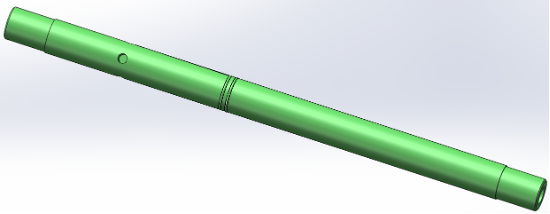
\includegraphics[width=0.7\textwidth]{figure/chapter3/inner-pipe-3-in-1.png}
	}
	\hfill
	\subfloat[抗拉强度分析]{%
	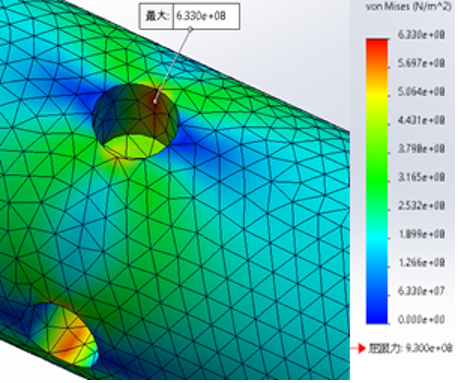
\includegraphics[width=0.4\textwidth]{figure/chapter3/inner-pipe-3-in-1-tensile-stress.png}
	}
	\vspace{1em}
	\subfloat[抗扭强度分析]{%
	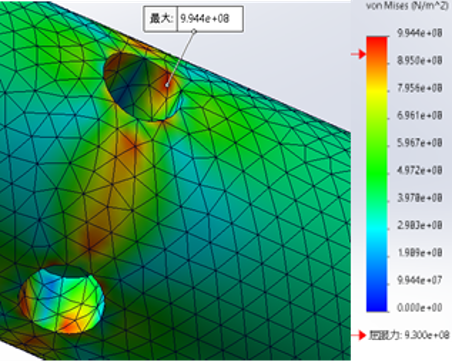
\includegraphics[width=0.45\textwidth]{figure/chapter3/inner-pipe-3-in-1-torsional-stress.png}
	}
	\caption{脉冲发生器薄弱零件强度有限元分析}
	\label{fig:FEA_inner_pipe_3_in_1}
\end{figure}

	\subsection{脉冲发生模块动力学模型及频率响应特性研究}
\subsubsection{脉冲发生模块流体-固体耦合机制及受力分析}

如图\ref{fig:working_cycle_pulse_module}所示，脉冲发生模块的工作工况主要分为四个阶段：

\begin{itemize}
	\item 蓄能阶段：当高压流体经由钻柱进入脉冲发生模块芯轴腔室时，由于侧向出水孔处于关闭状态，下方长开喷嘴具有节流效果，流体经过活塞腔入水孔进入腔室，腔室形成半封闭空间。随着泵入流量 的持续补充，流体被压缩，腔内静压力  迅速升高。
	\item 开启阶段：当液压力作用在活塞端面产生的推力超过弹簧预紧力及摩擦力之和时，活塞克服阻力向开启方向位移。当位移达到设计临界点 时，出水孔打开，活塞从出水孔打开处向上运动至最远点（速度为零处）。
	\item 喷射阶段：腔内高压流体瞬间经喷头排出，形成高速脉冲射流冲击井筒环空，活塞从最远点返回至侧向出水孔。 
	\item 复位阶段： 随着压力下降，弹簧势能释放，驱动活塞迅速复位至初始位置，关闭出水孔，系统进入下一个循环。
\end{itemize}

\begin{figure}[htbp]
	\centering
	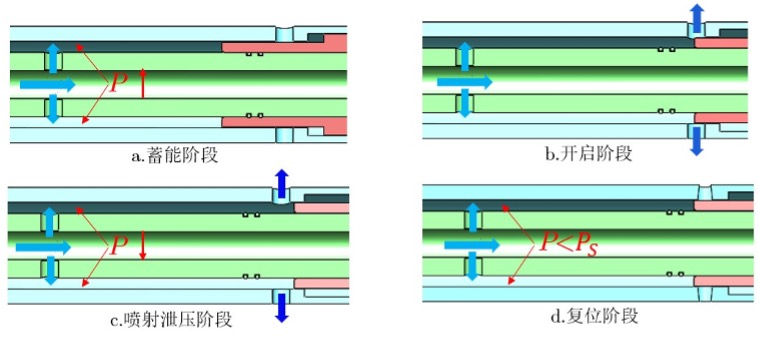
\includegraphics[width=0.9\textwidth]{figure/chapter3/working-cycle-pulse-module.jpg}
	\caption{脉冲发生模块工作周期示意图}
	\label{fig:working_cycle_pulse_module}
\end{figure}

（1）往复活塞受力模型

在活塞工作的任意周期瞬时$t$，往复活塞的运动状态取决于多种力场的综合作用—包括液压驱动力$F_p$，惯性力$F_a$，弹簧线性约束力$F_s$，粘性与摩擦阻力$F_d$。为了精确描述其动力学行为，建立如下受力平衡模型。

\begin{figure}[htbp]
	\centering
	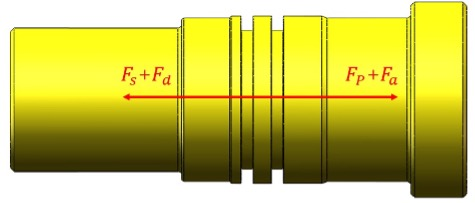
\includegraphics[width=0.6\textwidth]{figure/chapter3/force-analysis-reciprocating-piston.jpg}
	\caption{脉往复活塞受力分析图}
	\label{fig:force_analysis_reciprocating_piston}
\end{figure}

流体压力作用于活塞环形端面$A_1$。由于井下环境存在环空压力$P_{out}$，有效驱动力表现为内外压差：
\begin{equation}
	F_p(t)=\left[P(t)-P_{out}\right]\cdot A_1
\end{equation}
式中，$A_1$为活塞有效受压面积，其计算公式为：
\begin{equation}
	A_1=\frac{\pi}{4}\left(r_1^2-r_2^2\right)
\end{equation}
式中，$r_1$为活塞腔外径，m；$r_2$为活塞腔内径，m；

本装置采用高刚度矩形截面螺旋弹簧作为复位元件，在同等安装空间下可提供更大的恢复力，且其刚度特性受截面长宽比影响显著。根据材料力学及弹簧设计理论，矩形截面弹簧的等效刚度$k$可表征为：
\begin{equation}
	k=\frac{G\cdot b\cdot h^3}{n\cdot D^3} \eta
\end{equation}
式中，$G$为弹簧材料的弹性模量，Pa；

$b$为弹簧截面的径向宽度；

$h$为截面轴向高度；

$D$为弹簧的中径；

$n$为有效圈数；

$\eta$为形状修正系数，取决于长宽比$b/h$。

在脉冲发生模块工作过程中，弹簧力$F_s$随活塞位移$x(t)$呈线性变化关系：
\begin{equation}
	F_s(x)=k\cdot\left[x(t)+x_0\right]
\end{equation}

活塞在往复运动中受到密封件的干摩擦力$F_f$以及流体层间剪切产生的粘性阻尼力。为简化计算，通常采用等效粘性阻尼模型：
\begin{equation}
	F_d(t)=C\frac{dx(t)}{dt}
\end{equation}
式中，$C$为摩擦等效阻尼系数。

由于活塞在液体中高频振荡，会带动周围部分流体共同运动，从而产生惯性力$F_a$：
\begin{equation}
	F_a(t)=m\frac{d^2x(t)}{dt^2}
\end{equation}
式中，$m$为活塞及所有随动运动件的等效总质量，kg。

（2）流固耦合响应特性分析

脉冲发生模块的工作过程包括芯轴内腔的非稳态流场以及活塞运动两个方面，系统的动力学行为由流体压力场的变化与活塞的机械响应共同决定。

\begin{figure}[htbp]
	\centering
	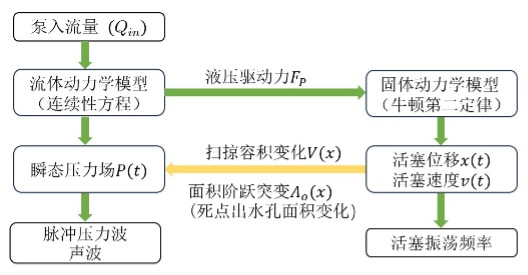
\includegraphics[width=0.7\textwidth]{figure/chapter3/FSI-logic.jpg}
	\caption{水力脉冲冲砂洗井工具脉冲发生模块结构图}
	\label{fig:FSI_logic}
\end{figure}

在脉冲循环中，流体与固体的相互作用主要体现在以下两个维度：

(1)压力对运动的驱动：随泵入流量$Q_{\mathrm{in}}$的积聚，腔室内流体被压缩，产生的瞬态压力$P(t)$作用于活塞端面$A_1$，形成驱动力$F_p$。当该力克服矩形弹簧预紧力及摩擦阻力后，改变活塞的运动状态。

(2)运动对压力的反馈：活塞的轴向位移$x$实时改变腔室的控制容积$V(t)$。当位移超过开启阈值$L$时，出水孔有效过流面积$A_o(x)$发生阶跃式变化，导致腔内流体迅速外泄，压力场随之重构。

系统的非线性特征主要源于开启时刻流道边界的突变。在活塞位移$x<L$时，系统处于蓄能阶段，流体处于高压状态；当$x>L$时，出水孔由封闭转为开启，系统边界由静态边界转变为自由出流边界。此时，活塞的往复运动会产生扫掠容积$A\cdot dx/dt$。在泄压阶段，活塞在矩形弹簧作用下迅速复位，其扫掠容积的方向与流体泄出方向相反，这种容积补偿效应是腔内形成瞬时负压物理过程的重要成因。

从能量角度分析，连续的流体压力能首先转化为弹簧的弹性势能与活塞的动能。在开启瞬间，由于矩形弹簧的高刚度特性，存储的能量在极短时间内释放，通过侧向出水孔转化为高速射流。这一过程伴随着剧烈的压力脉动，实现了对套管内壁及砂砾再沉积的振荡剥离。


\subsubsection{脉冲发生模块瞬态动力学模型构建}
在明确了脉冲发生模块内部流体与固体部件相互作用的物理机制后，为了能够定量分析脉冲发生模块在一个周期内活塞位移、速度随时间的变化关系，必须建立一套能够反映系统真实运动状态的数学模型。
根据流体连续性方程：

\begin{equation}
	Q = A_1\frac{dx}{dt}+Q_n
\end{equation}
式中，$A_1dx/dt$为用于推动活塞向上运动的体积变化率；$Q_n$为节流排量，$m^3/h$。

根据流体力学中的薄壁小孔流出模型，流经节流喷嘴的流量$Q_n$与缸内外压差$P(t)-P_{out}$的关系为
\begin{equation}
	Q_n=C_dA_n\frac{2(P(t)-P_{out})}{\rho_w}
\end{equation}
式中：$C_d$为喷嘴的流量系数，$A_n$为节流喷嘴的截面积，$m^2$，$\rho_w$为流体密度，$kg/m^3$。

由于$Q>>A_1\frac{dx}{dt}$，活塞运动对系统总流量的扰动微乎其微。将$Q_n$代入，则
\begin{equation}
	P(t)-P_{out}=\Delta P_{close}
\end{equation}


液压驱动力：
\begin{equation}
	\left(P(t)-P_{out}\right)\cdot A_1=\frac{A_1\rho_2}{2C_d^2A_n^2}Q^2
\end{equation}
取活塞初始静止位置为原点，其向下运动方向为正。活塞蓄能阶段的运动微分方程为：
\begin{equation}
	\frac{d^2}{dt^2}+C_1\left(\frac{dx}{dt}\right)^2+\left(C_2 x+C_3\right)\frac{dx}{dt}+C_4 x+ C_5 =0
\end{equation}

式中， $C_1$为非线性阻力系数，物体在流体中高速运动时，会产生与速度平方成正比的阻力：
\begin{equation}
	C_1=\frac{C_DA_2\rho_w}{2V\rho_f}
\end{equation}
$C_2$与$C_3$为粘性摩擦力阻尼，活塞与缸体之间存在微小的环空狭缝，当活塞运动时，流体在狭缝中产生剪切流动，这个摩擦力与运动速度成正比
\begin{equation}
	C_2=-\frac{2\mu\pi r_1}{\rho_f V\delta}
\end{equation}
\begin{equation}
	C_3=\frac{2\mu\pi\left(l_1r_1+l_2r_2\right)}{\rho_f V \delta}
\end{equation}
$C_4$为弹簧刚度与静水压恢复项：
\begin{equation}
	C_4=\frac{K}{\rho_f V}-\frac{\pi r_1 g \delta \rho_w}{\rho_f V}
\end{equation}
 $C_5$为常数驱动力项，不随时间、位移和速度改变：
 %这儿没写完
 
 式中：$r_1$为活塞腔外径，$m$；$r_2$为活塞腔内径，$m$；$C_D$为量纲阻力系数,它随着物体的形状和雷诺数而变，流体作用于流体的阻力大小与其成正比；$\rho_w$为流体密度，$kg/m^3$；$\rho_f$为活塞密度，$kg/m^3$；$K$为弹簧刚度，$N/m$；$V$为活塞体积，$m^3$；$\delta$为活塞与缸体之间的间隙，$m$；$l_1$为从侧向出水孔到活塞下端距离，$m$；$l_2$为活塞总长度，$m$；$\mu $，流体粘度，$Pa\cdot s$；$g$为重力加速度，$m/s^2$。
 
 活塞开启阶段的运动微分方程为：
 
 式中：
 
 %有两个方程没写出来。
 
 其中：当活塞位移到侧向出水流孔打开时，此时流体有了两条并行的通道：节流喷嘴$A_n$和侧向出水孔孔（设其流通面积为$A_h$）。由于总泄流面积增加，系统压力瞬间卸载，导致压差下降：
 %这里缺一个方程
 
 活塞喷射阶段的运动微分方程为：
  %这里缺一个方程
  
  式中：
  %这里缺一个方程
  %这里缺一个方程
活塞复位阶段的运动微分方程为：

%这里缺一个方程

式中：


把四个阶段活塞的运动微分方程联立：


活塞各个运动阶段所满足的初始条件分别为：

式中：$h$为侧向出水孔距活塞下端的距离，$\mathrm{m}$；$h_1$为活塞运动的最高点高度，$\mathrm{m}$；$v_1$为上升时活塞运动到侧向出水孔处的速度，$\mathrm{m/s}$；$v_2$为下降时活塞运动到侧向出水孔处的速度，$\mathrm{m/s}$。

根据上述模型及定解条件即可确定出脉冲发生模块的脉冲周期,以及在脉冲过程中任意时刻活塞的运动速度、位置等参数[68-69]。

本节通过研究了脉冲发生模块内部流场与固体组件受力特性，构建了描述其动力学行为的非线性常微分方程组。该模型以活塞运动微分方程为核心，联立腔室流体连续性方程，定量刻画了泵入流量 、下接头喷嘴泄流 以及矩形弹簧刚度对脉冲频率的协同作用机制，为后续揭示结构参数对系统振荡频率奠定了严谨的数学基础。

\subsubsection{关键设计参数对脉冲发生模块动力学特性的影响规律}

为验证系统非线性动力学模型的准确性，并揭示脉冲发生模块的瞬态运动规律，提取排量$Q=50\mathrm{m^3/h}$，侧向出水孔高度$l_1=75\mathrm{mm}$，弹簧刚度$K=757176\mathrm{N/m}$下活塞位移与速度随时间的响应特性曲线。

如图\ref{fig:piston_displacement_VS_time}所示，活塞从初始位置($x=0$)启动，在节流喷嘴产生的节流压差作用下加速向下运动，在$t=6.08\mathrm{ms}$时，活塞位移达到$75\mathrm{mm}$(侧向出水孔位置)，该阶段耗时约占整个周期的47.3（单位是什么）。活塞越过$75\mathrm{mm}$刻度线后，侧向出水孔打开，缸内流体压力骤降导致主驱动力消失，活塞在复位弹簧的作用下减速。在$t=7.75\mathrm{ms}$时，活塞速度降至零，活塞唯一达到整个周期最大冲程$88.13\mathrm{mm}$。活塞在最大冲程处复位，由被压缩的弹簧释放弹性势能驱动其向上回程。在$t=9.44\mathrm{ms}$时，活塞向上退回并再次经过$75\mathrm{mm}$位置，由于伴随有残余液压力及向下的重力阻碍，回弹段的曲线斜率略低于下击段。活塞向上越过侧向出水孔致其关闭，缸内瞬间重新憋起高压，形成液压阻力。 在$t=12.86\mathrm{ms}$时，活塞回落至$0\mathrm{mm}$的初始位置。从位移响应曲线可知，在 $Q=50\mathrm{m^3/h}$排量下，系统单次工作周期为$12.86\mathrm{ms}$，对应的工作频率为$77.76\mathrm{Hz}$。

\begin{figure}[htbp]
	\centering
	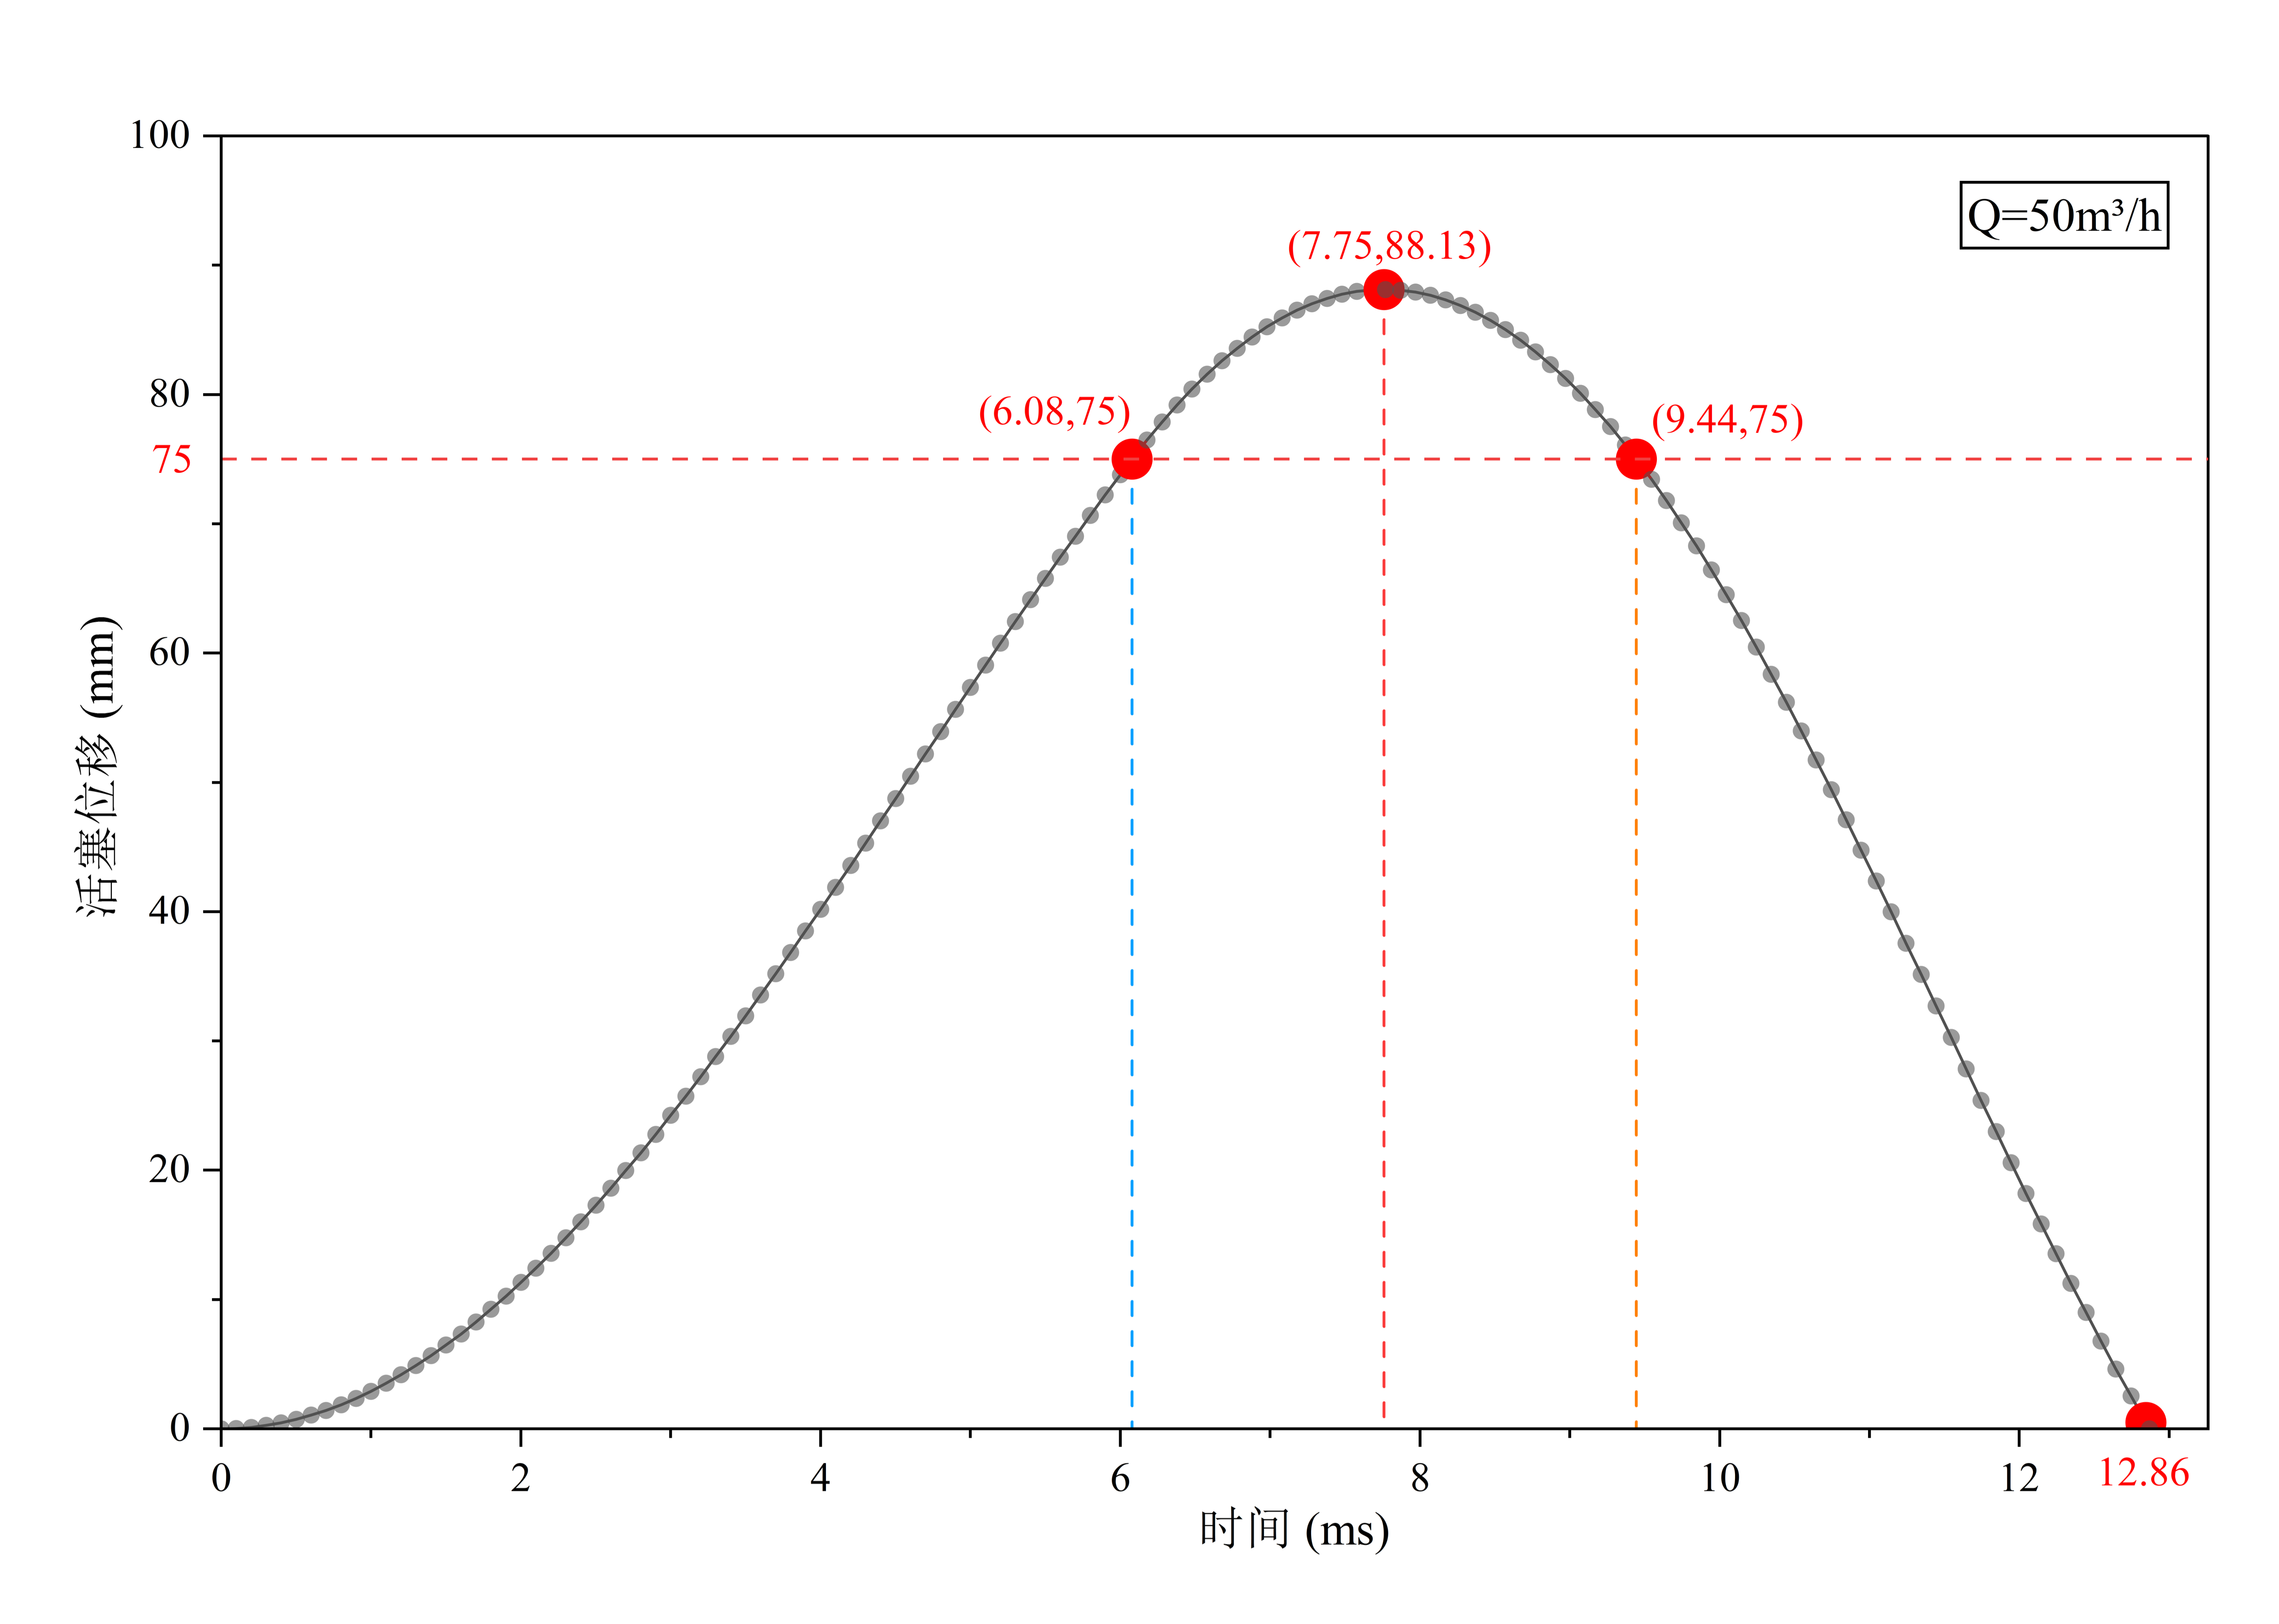
\includegraphics[width=0.7\textwidth]{figure/chapter3/piston-displacement-VS-time.png}
	\caption{活塞位移随时间变化曲线}
	\label{fig:piston_displacement_VS_time}
\end{figure}

如图\ref{fig:piston_velocity_VS_time}所示，活塞启动后，在压差作用下速度迅速增加，在$t=4.6\mathrm{ms}$时，活塞正向速度达到最大$17.26\mathrm{m/s}$。之后，由于弹簧被压缩，弹簧的弹性恢复力使活塞开始减速，在$t=6.08\mathrm{ms}$时，速度曲线的斜率出现了一个极其明显的折点， 标志着侧向出水孔被瞬间触发打开。液压驱动力发生减小，系统加速度突变为极大的负值。在纯机械弹簧力的强力压迫下，活塞速度在$1.68\mathrm{ms}$内从十多米每秒骤降至零，$t=7.75\mathrm{ms}$到达冲程死点）。经过下死点后，活塞速度变为负值（活塞向上运动），负向速度持续攀升，并在$t=11.44\mathrm{ms}$时刻达到整个周期的速度绝对值极值$-24.37\mathrm{m/s}$。在达到最大负向速度后，曲线斜率发生偏折，速度在初始限位和压差的作用下降为零。

\begin{figure}[htbp]
	\centering
	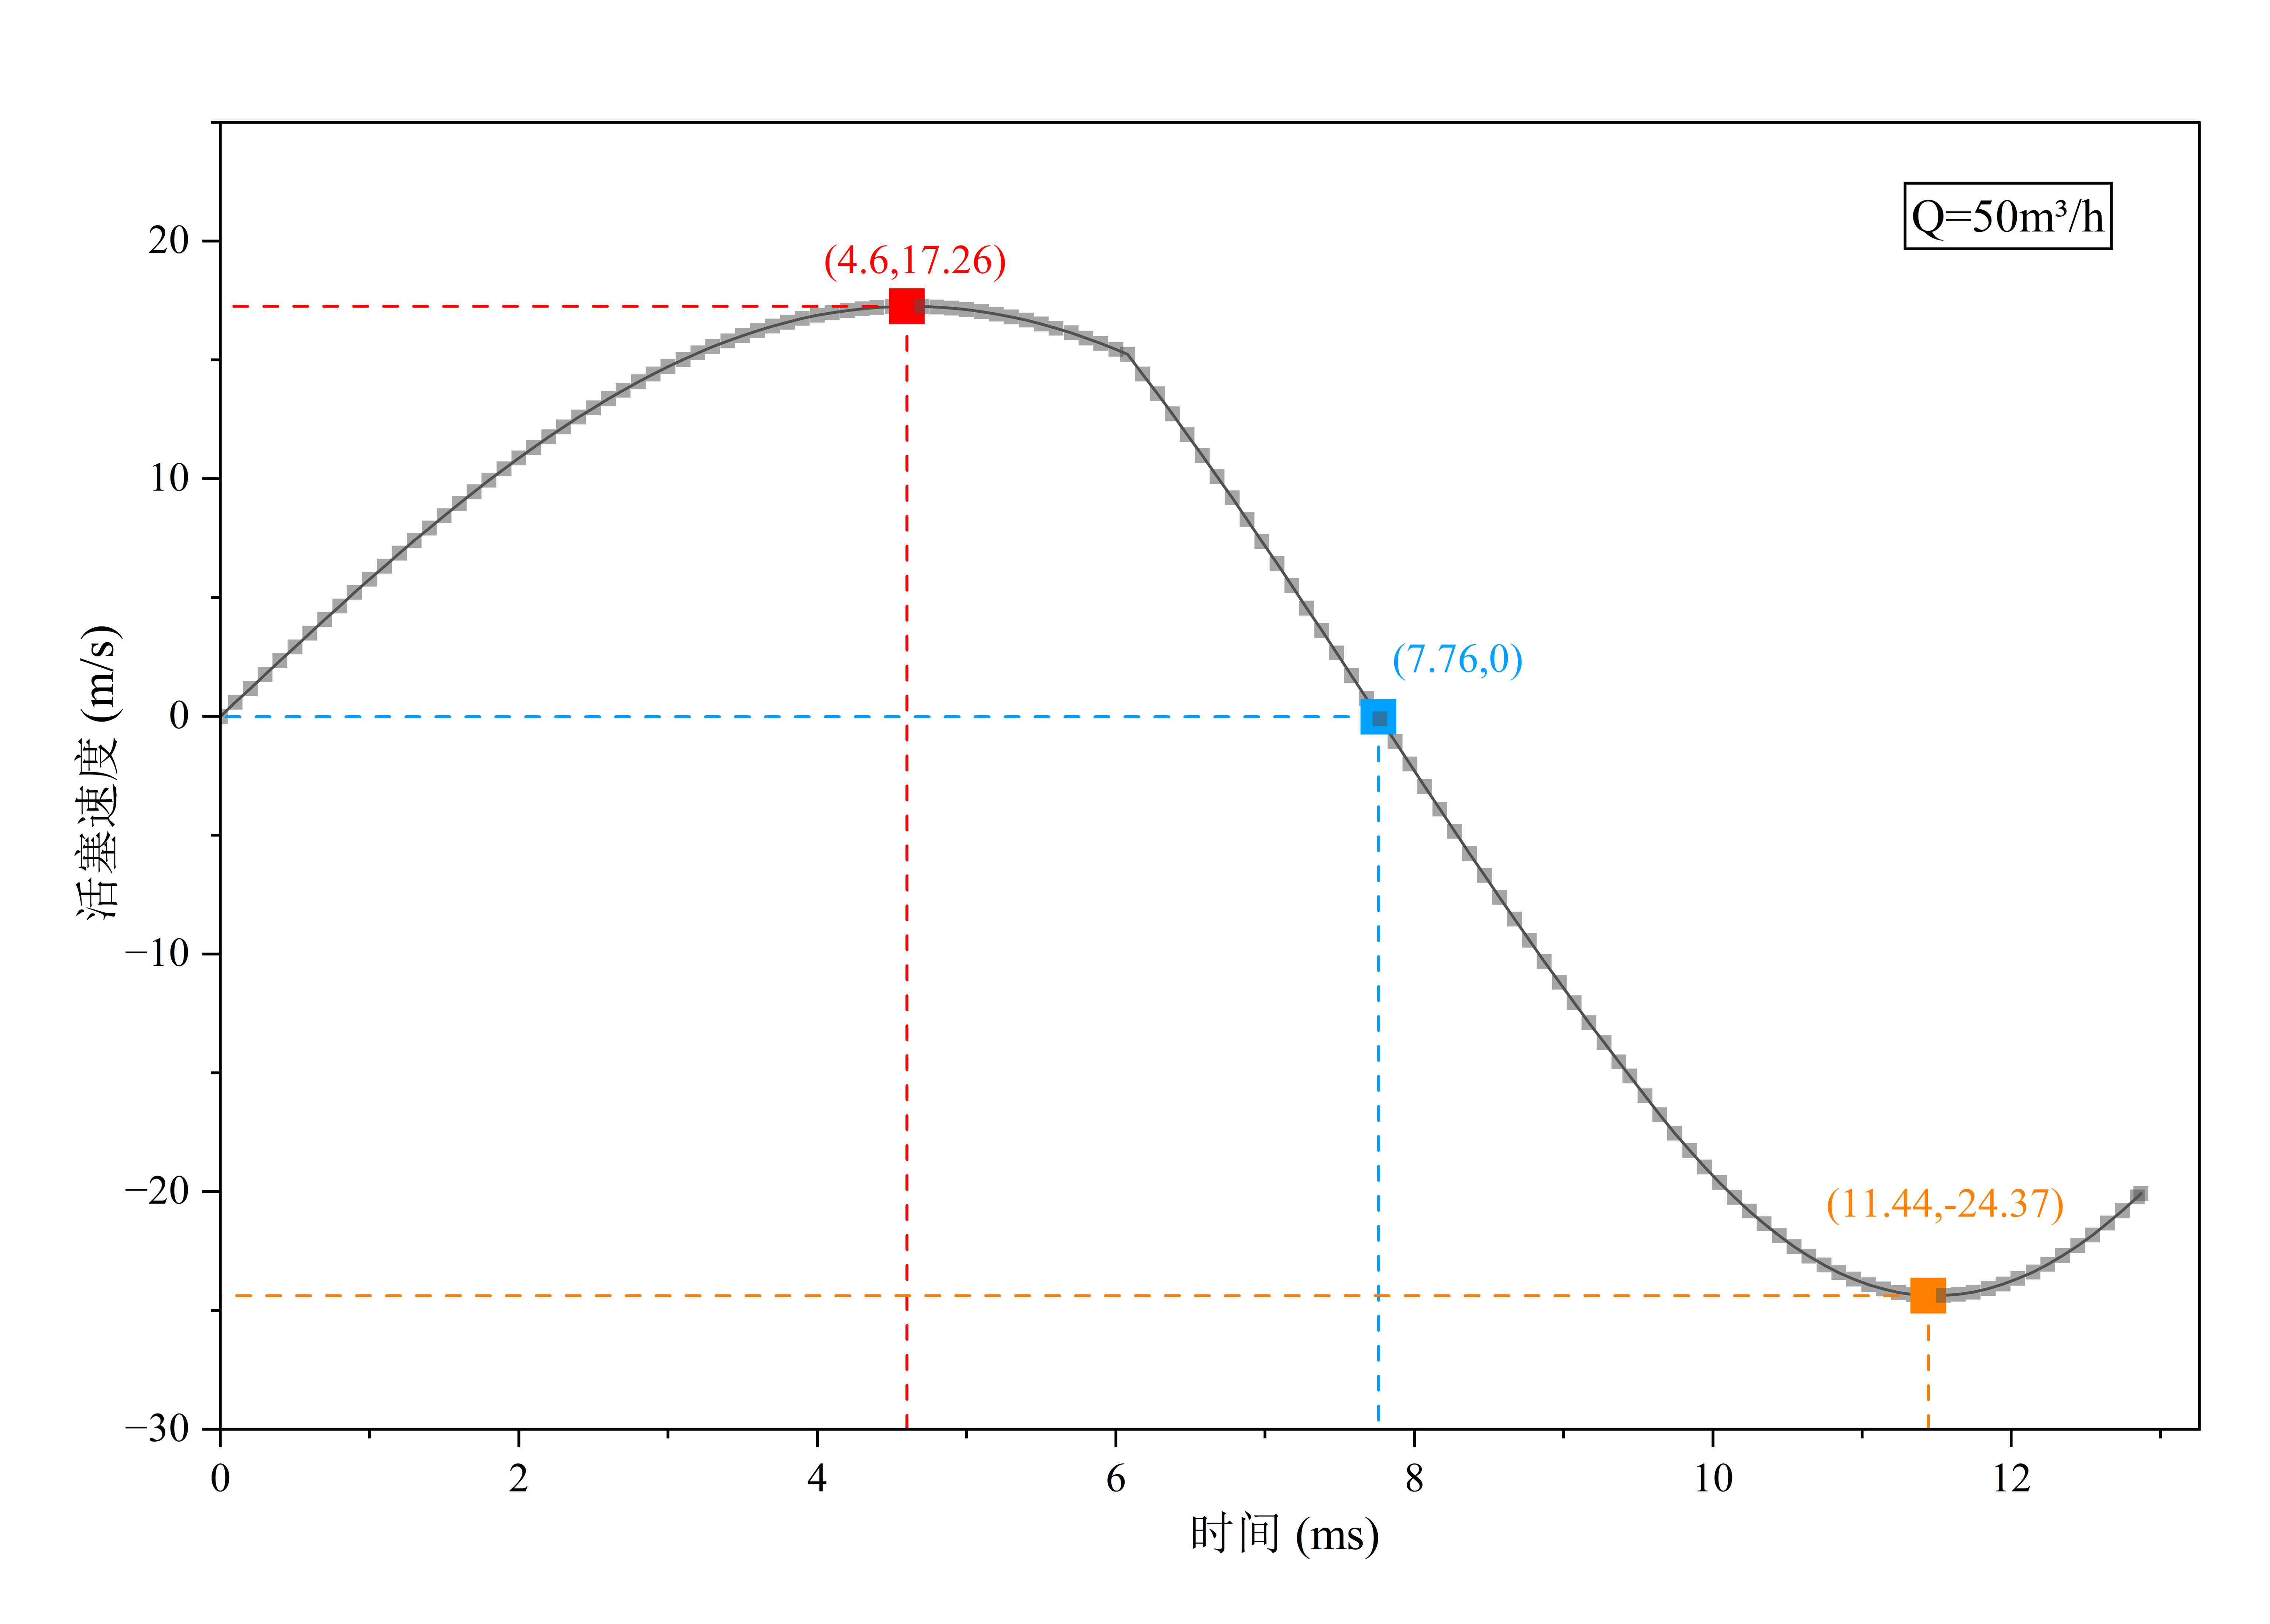
\includegraphics[width=0.7\textwidth]{figure/chapter3/piston-velocity-VS-time.png}
	\caption{活塞速度随时间变化曲线}
	\label{fig:piston_velocity_VS_time}
\end{figure}


（1）排量对脉冲发生模块频率的影响

排量$Q$是脉冲发生模块作业的关键参数，为揭示输入流量对系统动态特性的影响规律，本节在$46\mathrm{m^3/h}$至$58\mathrm{m^3/h}$的工作区间内，以$2\mathrm{m^3/h}$为梯度，绘制了活塞位移与速度随时间变化曲线对比图\ref{fig:piston_displacement_VS_Q}。对比发现：

随着排量$Q$增加，活塞的最大冲程呈显著的非线性单调递增趋势。从图中可以看到，排量越大的曲线，其上升斜率越大，且位移越早达到侧向出水孔位置。同时，在曲线的右侧末端，排量越大的曲线越早回归零点。尽管活塞位移上升阶段各曲线分离明显，但在越过峰值后的复位阶段，各组曲线下降斜率差异较小，均极其平滑地收敛于初始位置。

\begin{figure}[htbp]
	\centering
	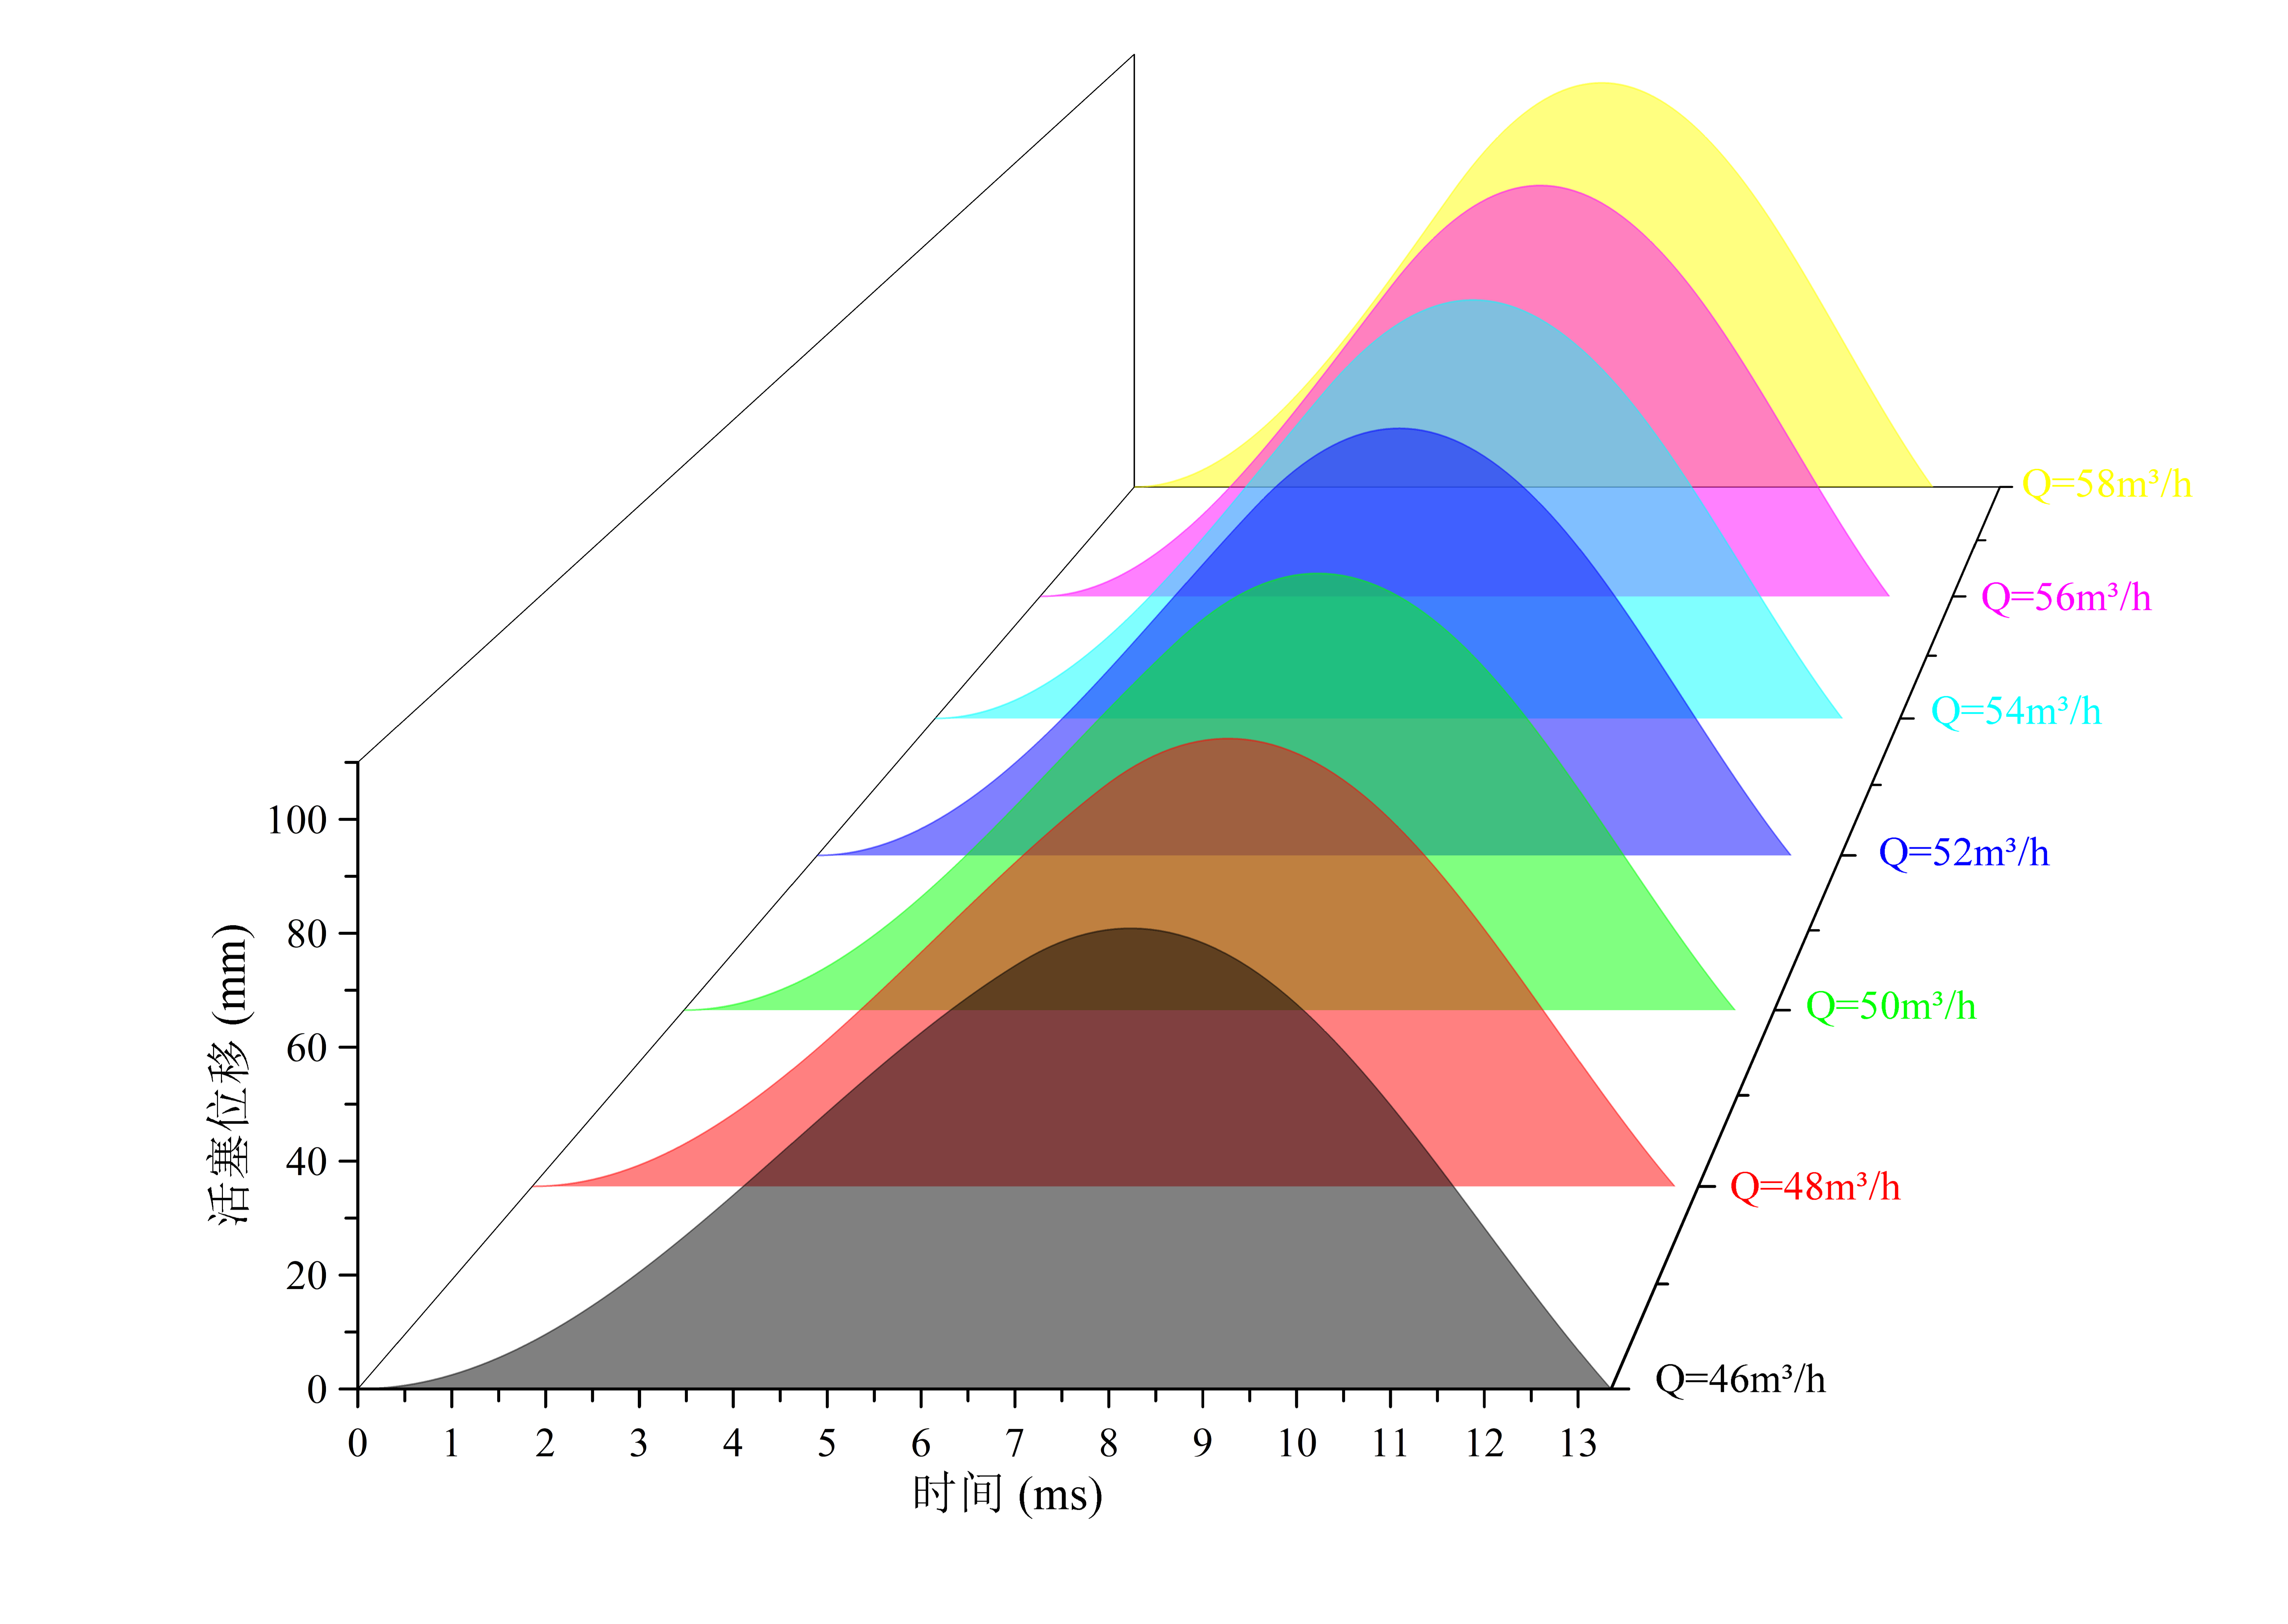
\includegraphics[width=0.7\textwidth]{figure/chapter3/piston-displacement-VS-Q.png}
	\caption{活塞位移随排量$Q$变化曲线对比图}
	\label{fig:piston_displacement_VS_Q}
\end{figure}


活塞速度随排量$Q$变化曲线如图\ref{fig:piston_velocity_VS_Q}所示，观察速度曲线的正向速度区，随着排量$Q$增加，速度曲线的波峰不仅在幅值上显著拔高（从$46m^3/h$的$14.5m/s$到$58m^3/h$的$23.1m/s$，且峰值出现的时间节点明显向左偏移。观察速度曲线的负向速度区，各排量下的弹簧回弹阶段均出现波谷。排量$Q$越大，负向速度的绝对值越大。在正向速度向负向速度过渡的速度零点，随着排量$Q$增加，曲线穿越时间轴的斜率变得越大。同时，整个速度波形的跨度沿时间轴显著缩短.

\begin{figure}[htbp]
	\centering
	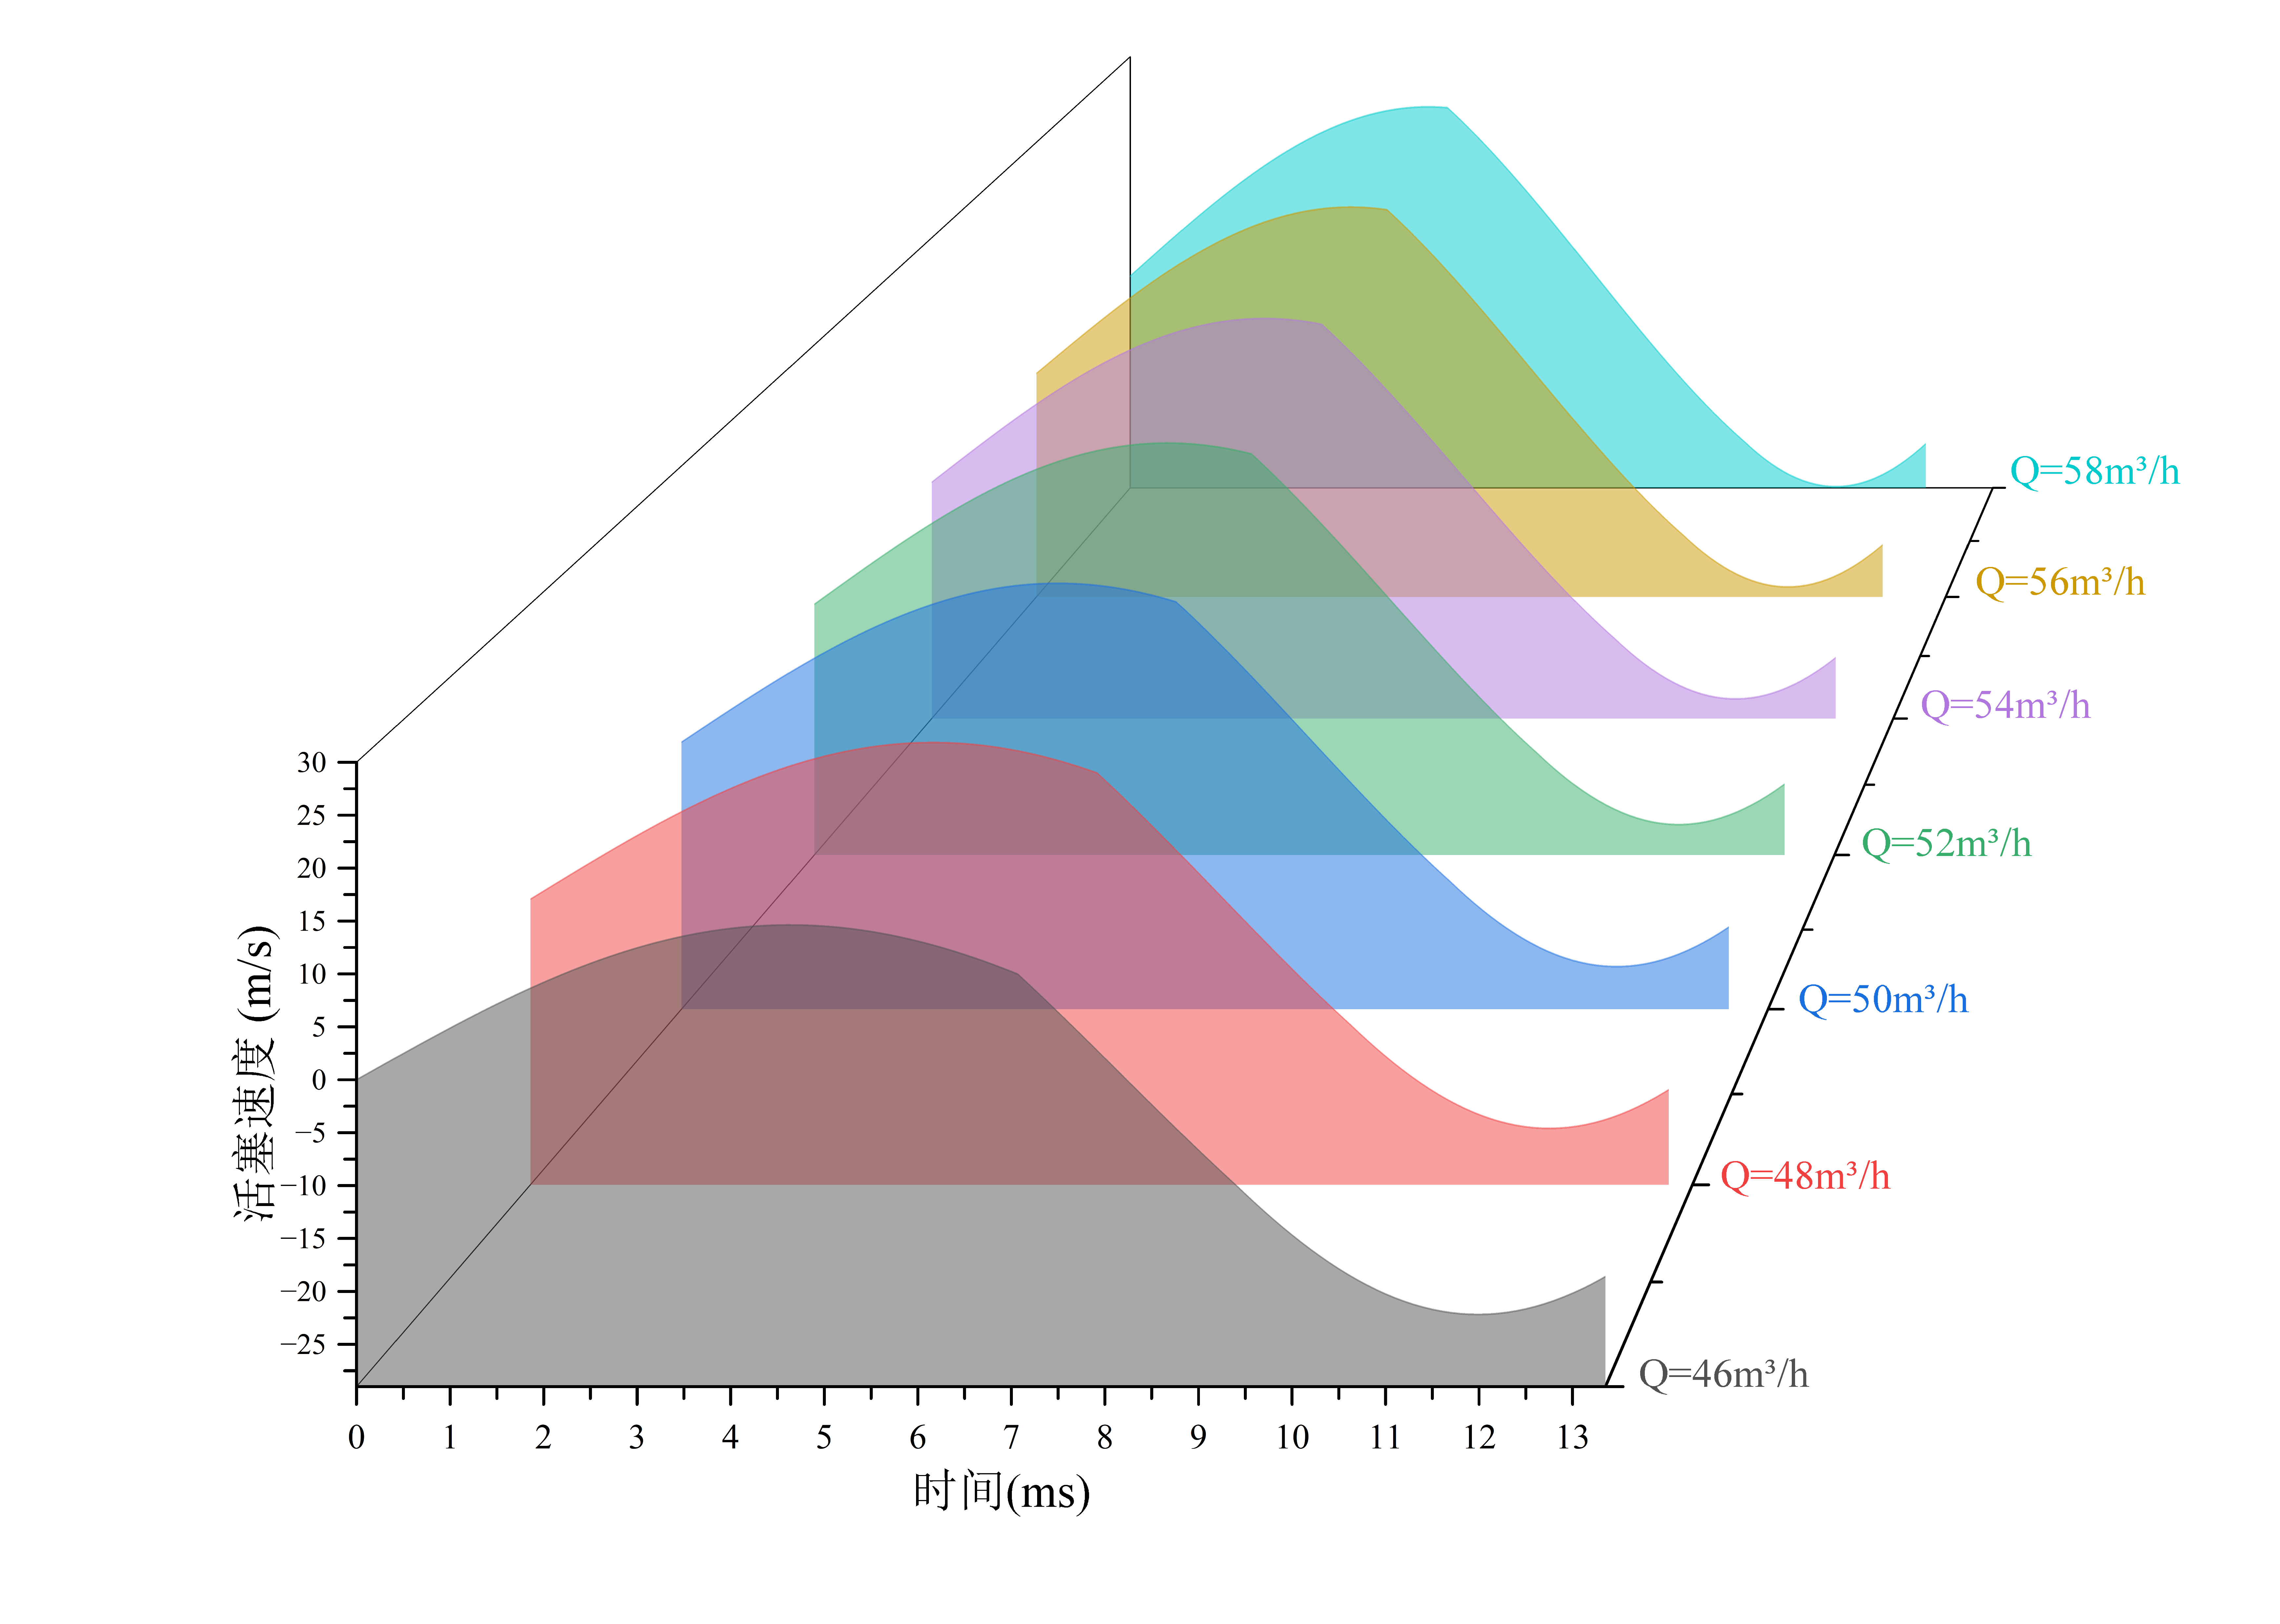
\includegraphics[width=0.7\textwidth]{figure/chapter3/piston-velocity-VS-Q.png}
	\caption{活塞速度随排量$Q$变化曲线对比图}
	\label{fig:piston_velocity_VS_Q}
\end{figure}

脉冲发生模块排量与工作频率、冲程关系特征曲线如图\ref{fig:pulse_module_frequency_stroke_VS_Q}所示，由图可知，在额定工作区间内，活塞最大冲程对流量 的变化极其敏感，且呈现出高度稳定的准线性增长趋势。提高流量能有效提升脉冲发生模块的工作频率 ，但其演化轨迹表现出明显的非线性特征。

\begin{figure}[htbp]
	\centering
	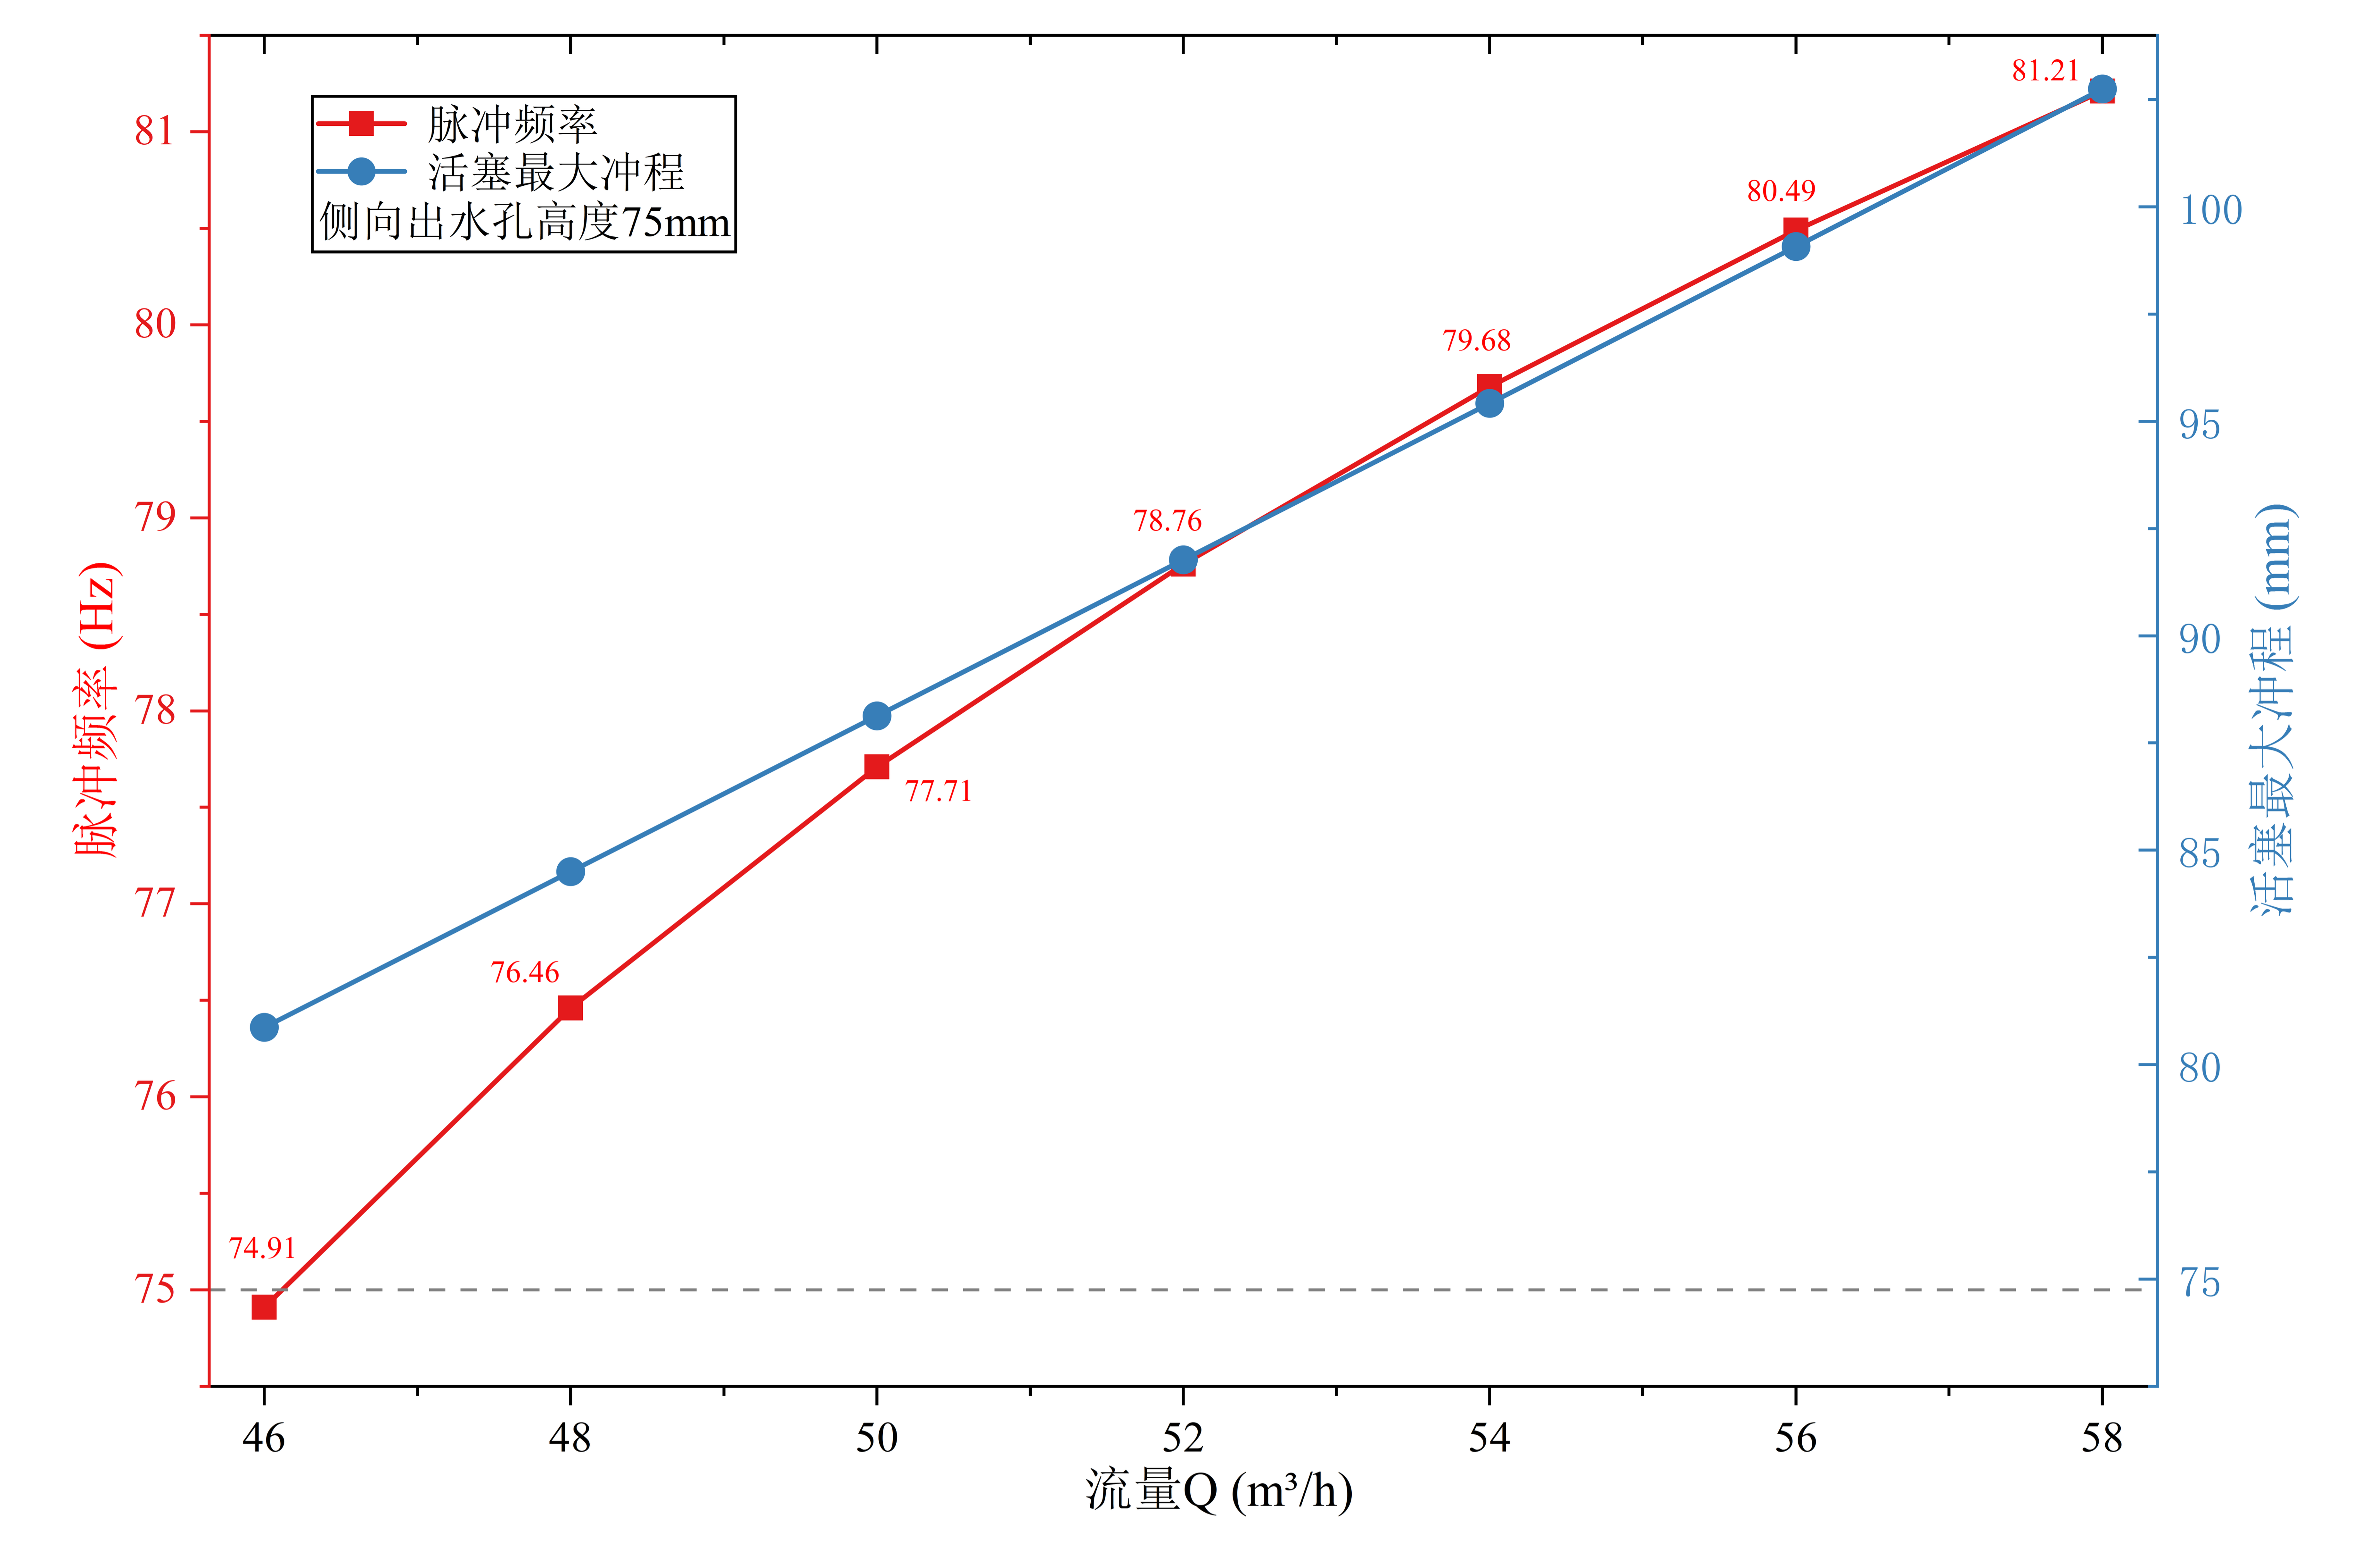
\includegraphics[width=0.7\textwidth]{figure/chapter3/pulse-module-frequency-stroke-VS-Q.png}
	\caption{脉冲发生模块排量与工作频率、冲程关系特征曲线}
	\label{fig:pulse_module_frequency_stroke_VS_Q}
\end{figure}

（2）矩形弹簧刚度对脉冲发生模块频率的影响

弹簧刚度$K$是脉冲发生模块结构设计的关键参数，为揭示弹簧刚度$K$对系统动态特性的影响规律，本节在$K=557176N/m$至$857176N/m$的设计区间内，以$50000N/m$为梯度，绘制了活塞位移与速度随时间变化曲线对比图\ref{fig:piston_displacement_VS_spring_K}。对比发现，随着弹簧刚度$K$的逐级递增，活塞位移波峰高度呈现出明显的阶梯式下降。在输入排量$Q$保持不变的前提下，高刚度弹簧能够以更短的变形距离吸收完相同的流体动能，从而使活塞最大冲程减小。观察时间轴可以发现，活塞刚度越大，其波形越窄，且波峰到达的时间节点整体向左侧发生偏移。刚度增加使活塞复位阶段动力增大，位移下降曲线斜率增大，减少了单次循环的时间。

\begin{figure}[htbp]
	\centering
	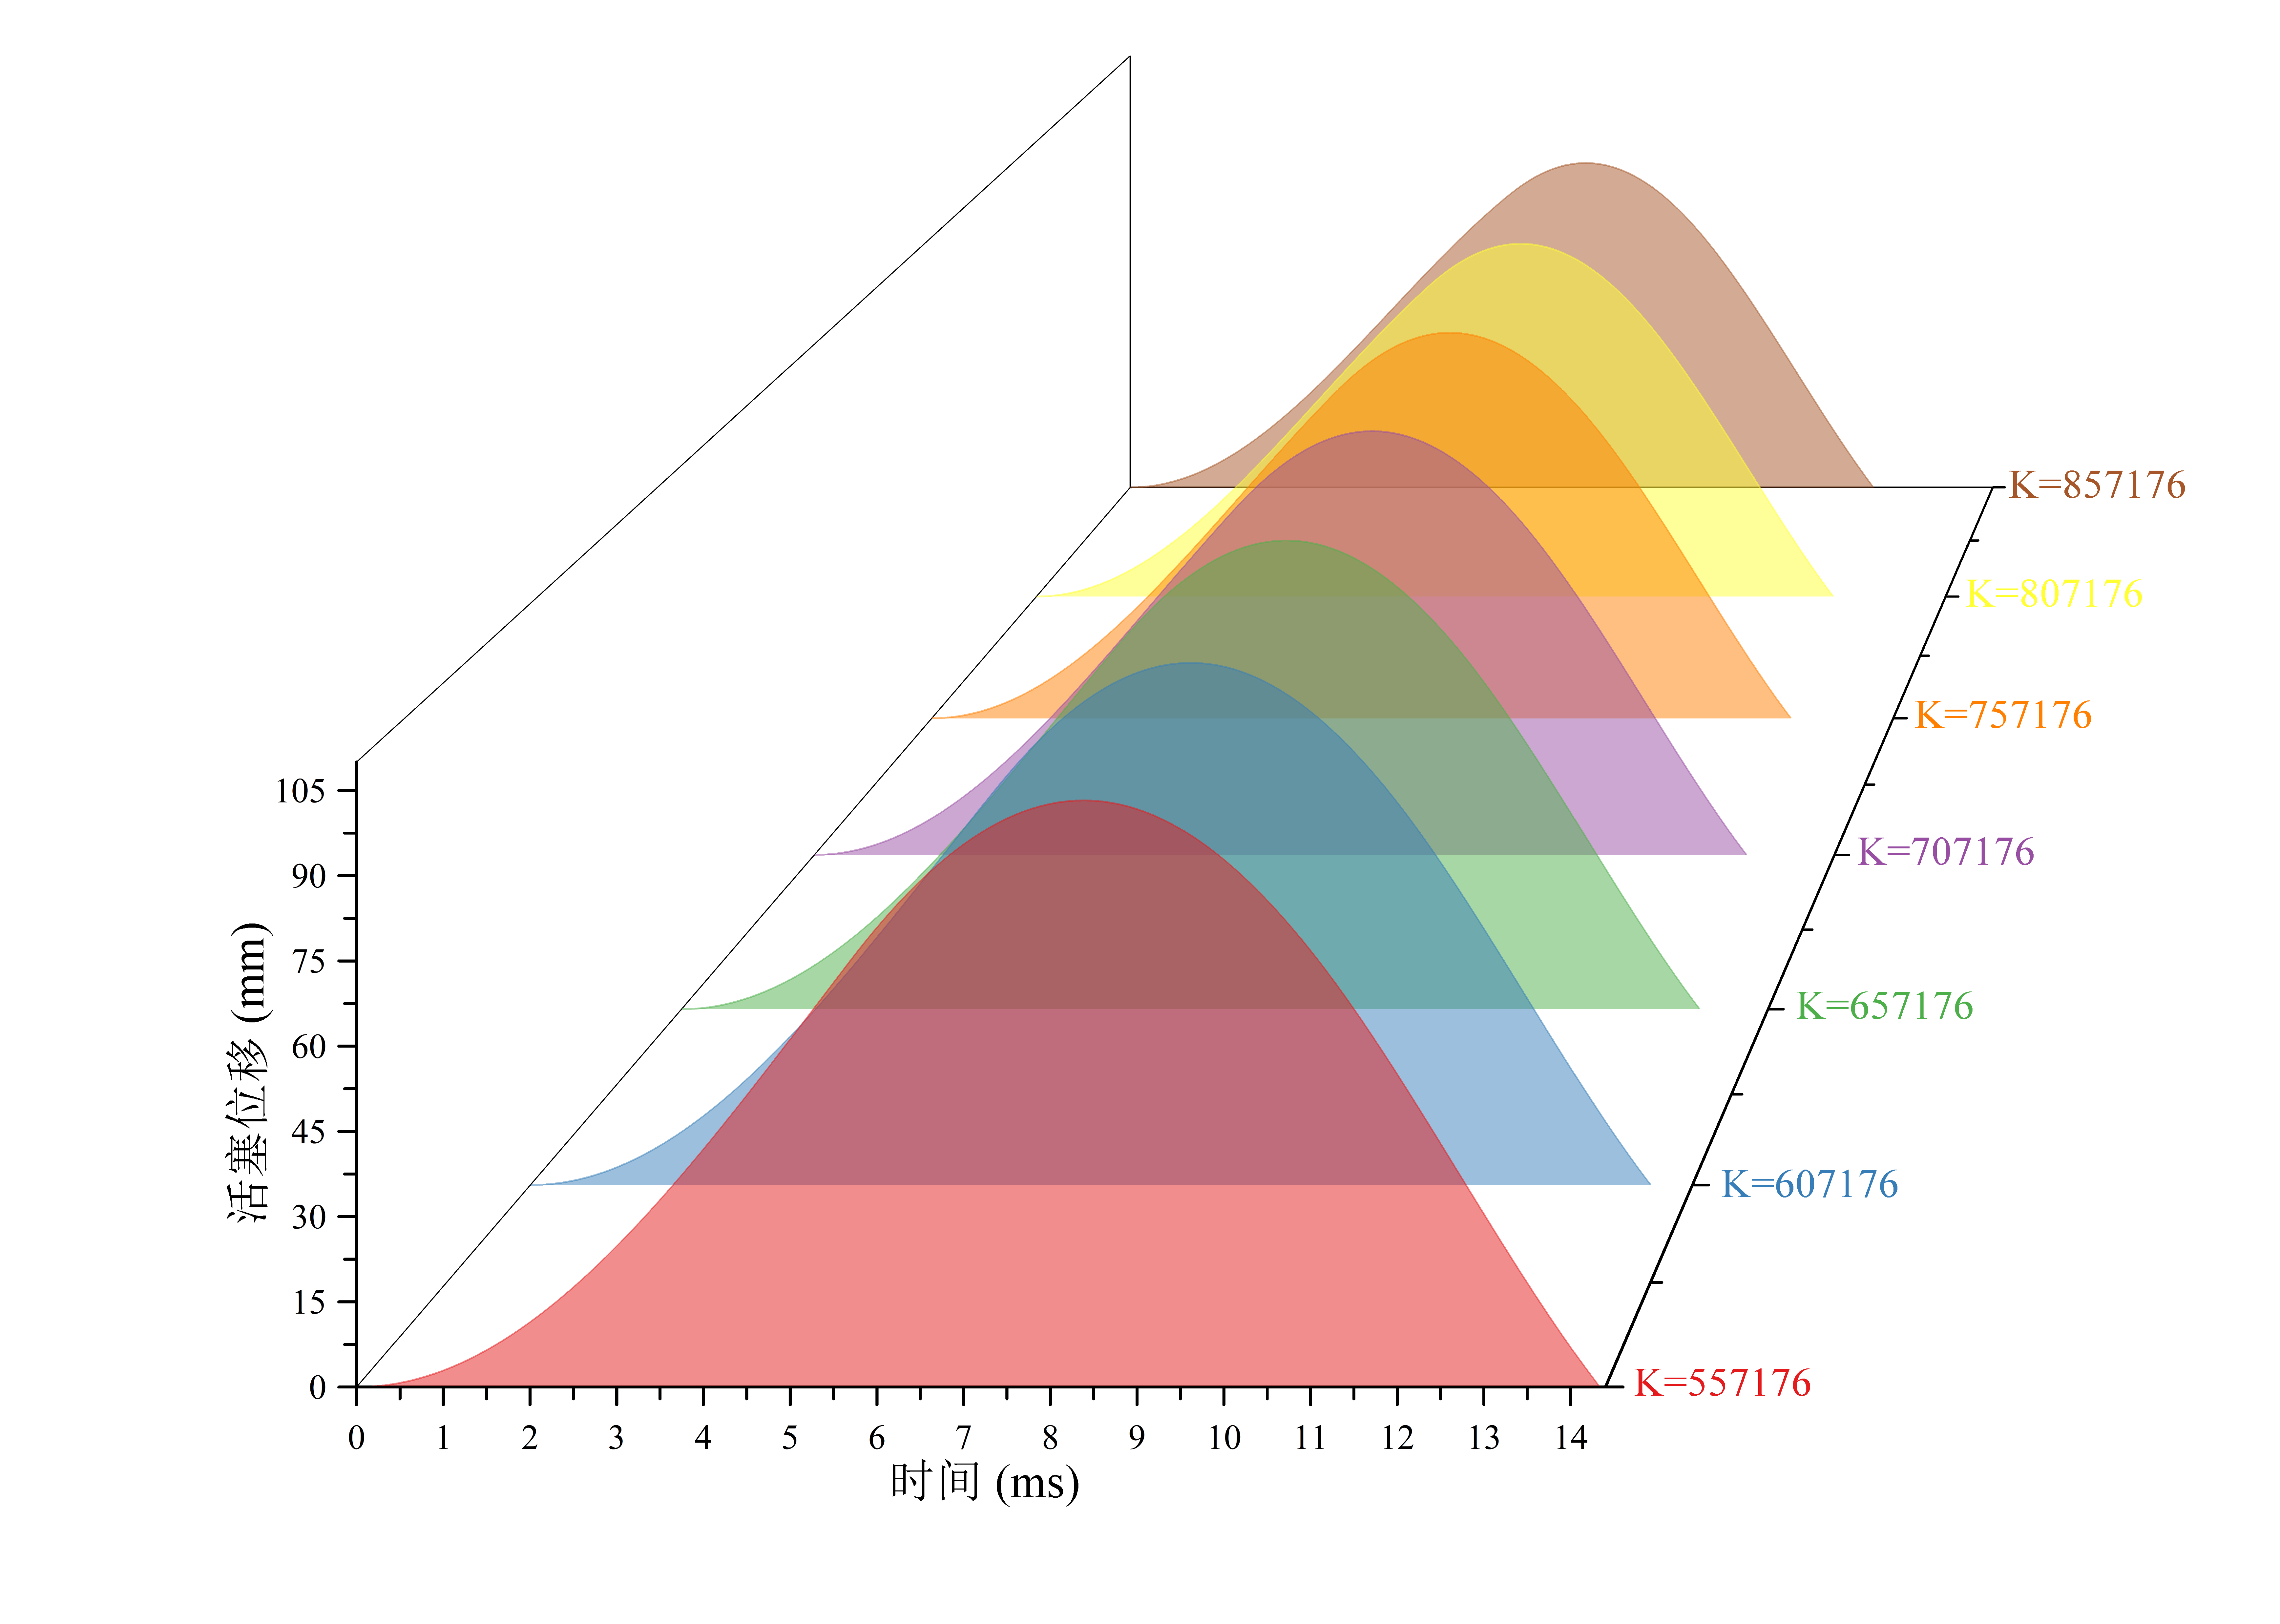
\includegraphics[width=0.7\textwidth]{figure/chapter3/piston-displacement-VS-spring-K.png}
	\caption{脉冲发生模块排量与工作频率、冲程关系特征曲线}
	\label{fig:piston_displacement_VS_spring_K}
\end{figure}

如图\ref{fig:piston_velocity_VS_spring_K}所示，随着弹簧刚度$K$的逐级递增，正向速度的波峰高度呈现阶梯式衰减，且波峰出现的时刻逐渐向左侧偏移。弹簧刚度$K$的增大使弹簧的压缩阻力增大，导致活塞正向最高速度下降，同时也使系统更早达到受力平衡点，从而表现为速度峰值的相位超前。随着弹簧刚度$K$的逐级递增，弹簧的弹性恢复力越大，活塞达到最大位移后，速度下降的斜率越大。随着弹簧刚度$K$的逐级递增，活塞的负向最高速度反而减小。尽管高刚度弹簧的初始回弹加速度更大，但由于其限制了活塞的最大冲程，导致其整体蓄积的弹性势能和可供加速的复位距离双双受限。

\begin{figure}[htbp]
	\centering
	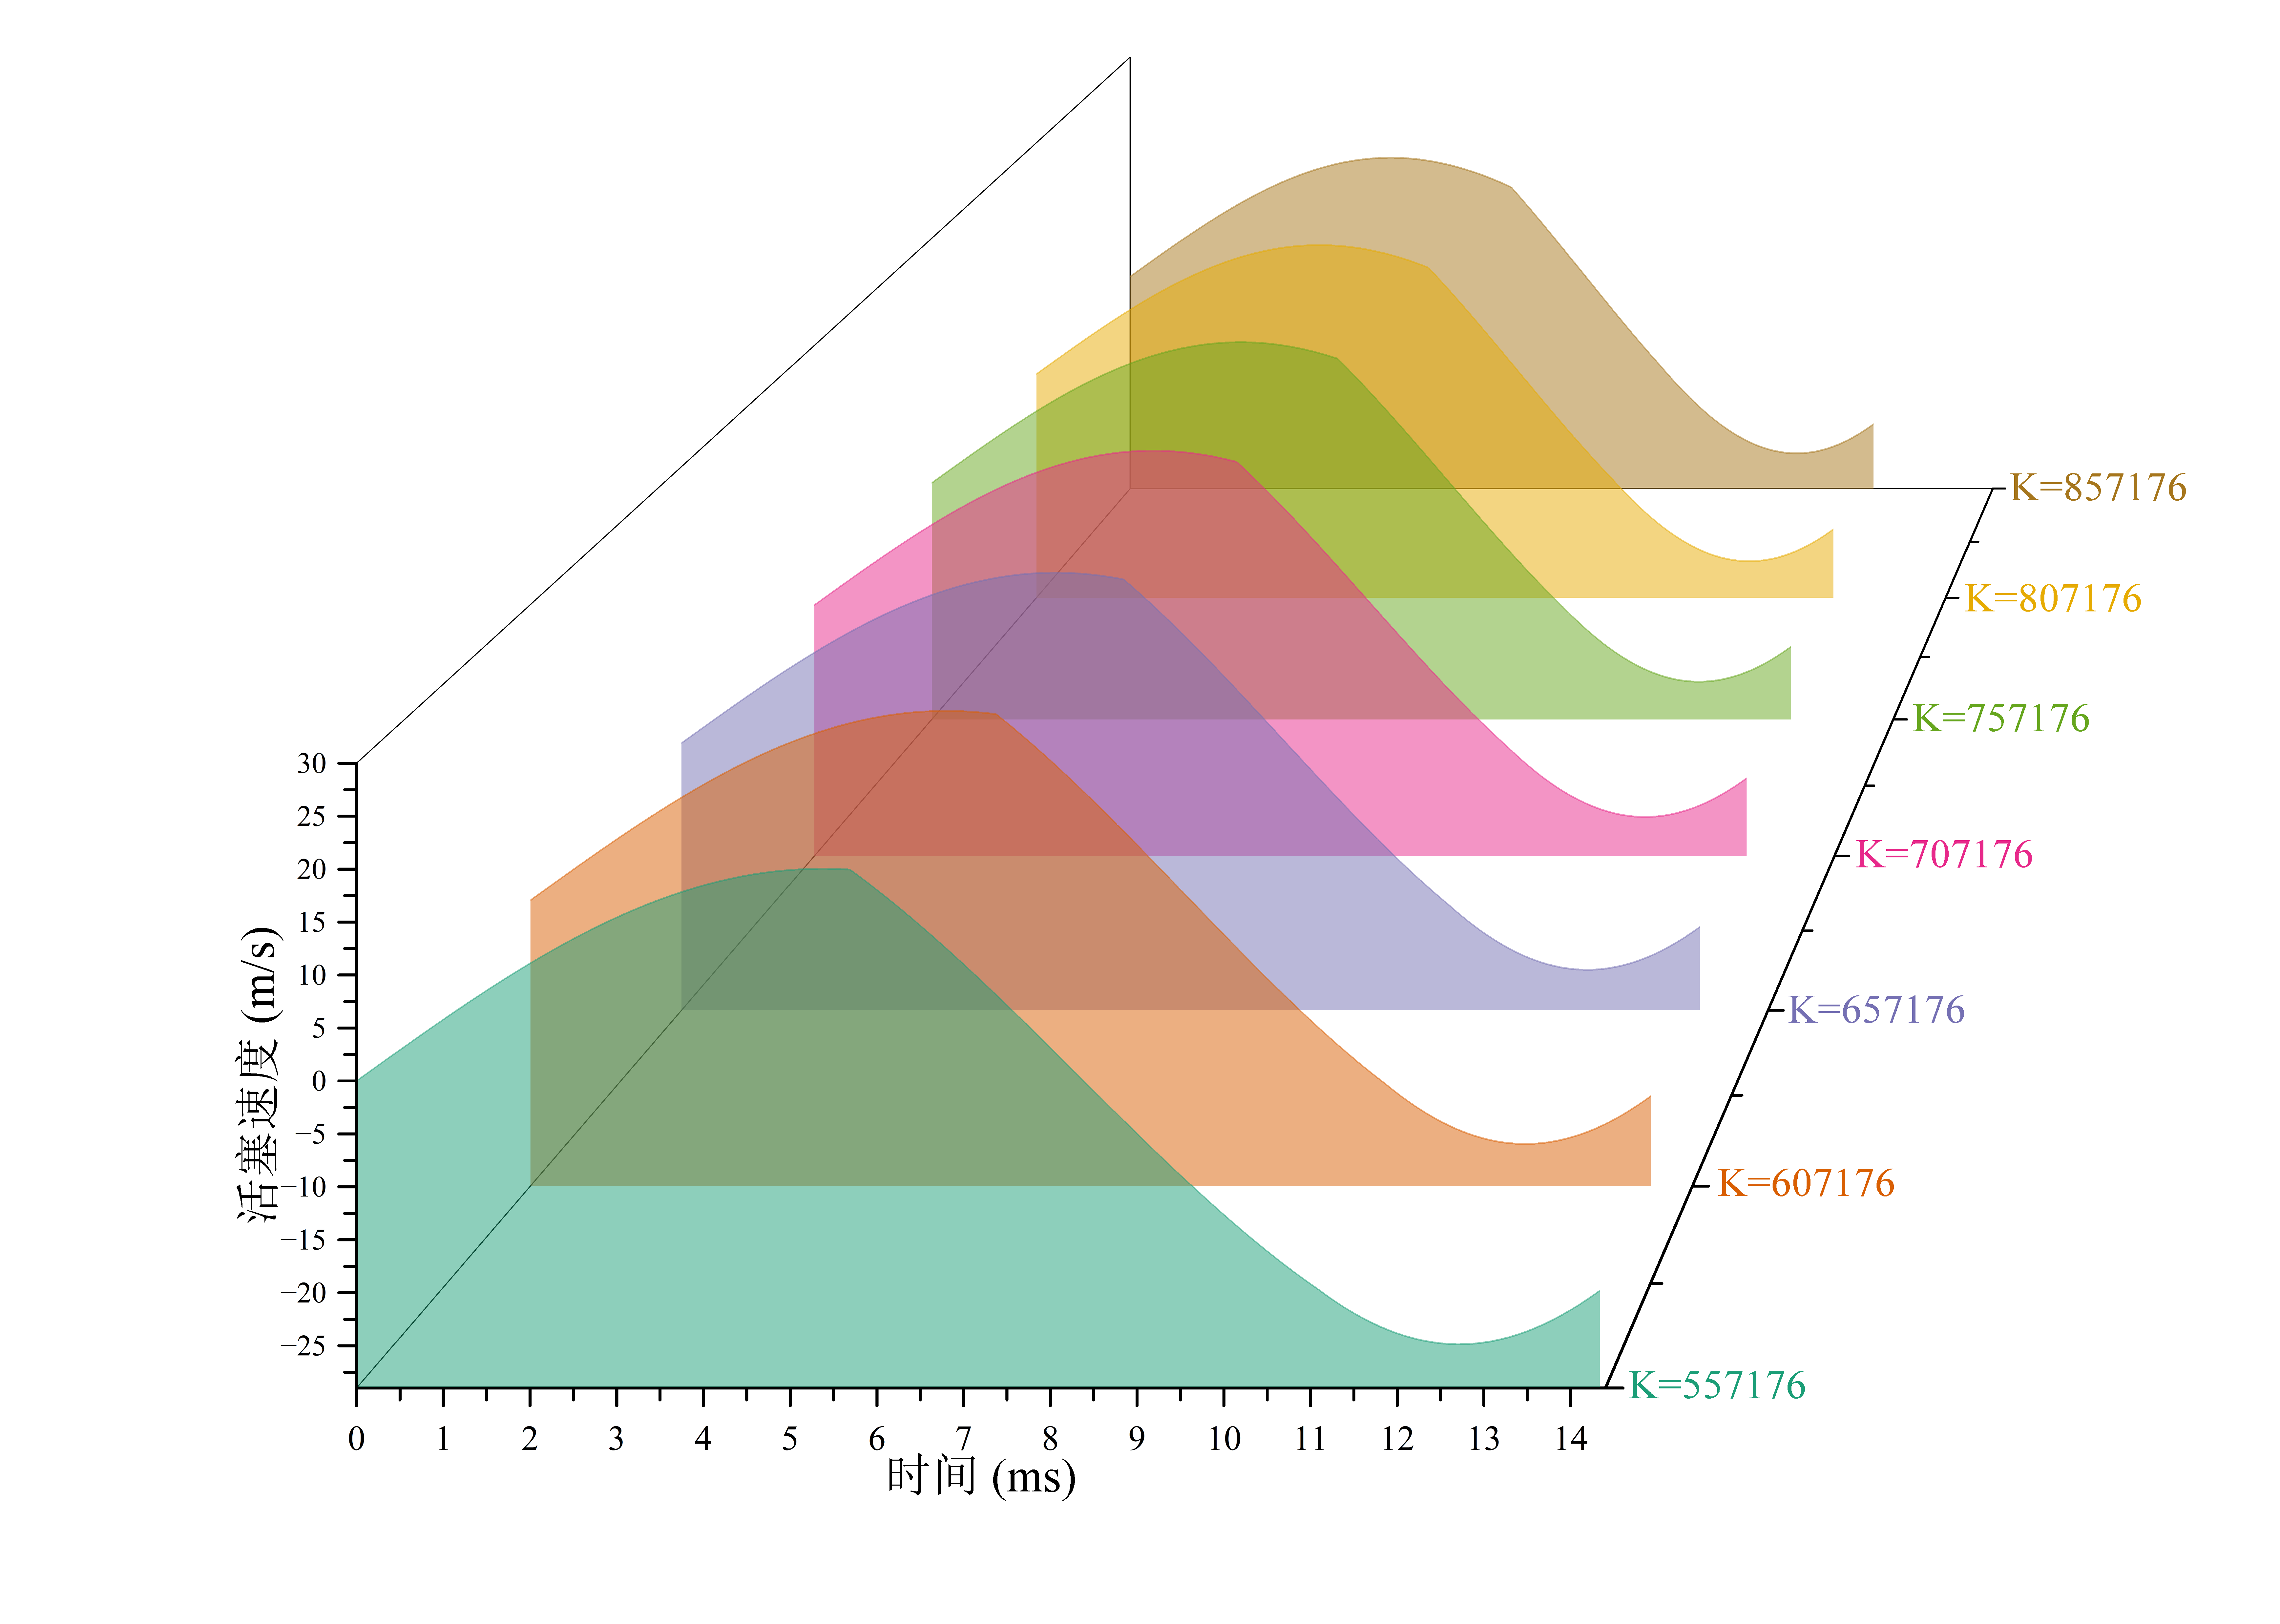
\includegraphics[width=0.7\textwidth]{figure/chapter3/piston-velocity-VS-spring-K.png}
	\caption{活塞速度随弹簧刚度$K$变化曲线对比图}
	\label{fig:piston_velocity_VS_spring_K}
\end{figure}

脉冲发生模块弹簧刚度$K$与工作频率、冲程关系特征曲线如图4.16所示，由图可知，随着弹簧刚度的逐级递增，活塞冲程呈现单调递减趋势。与冲程规律相反，工作频率随弹簧刚度的增加而增大。观察频率曲线的斜率可以发现，在低刚度向中等刚度过渡时，提频效果最为显著；但随着刚度进一步向$850kN/m$以上逼近，曲线爬升趋势放缓。这表明单纯依靠增加机械刚度来提频存在物理极限，过度强化刚度会反向制约下击效率。

\begin{figure}[htbp]
	\centering
	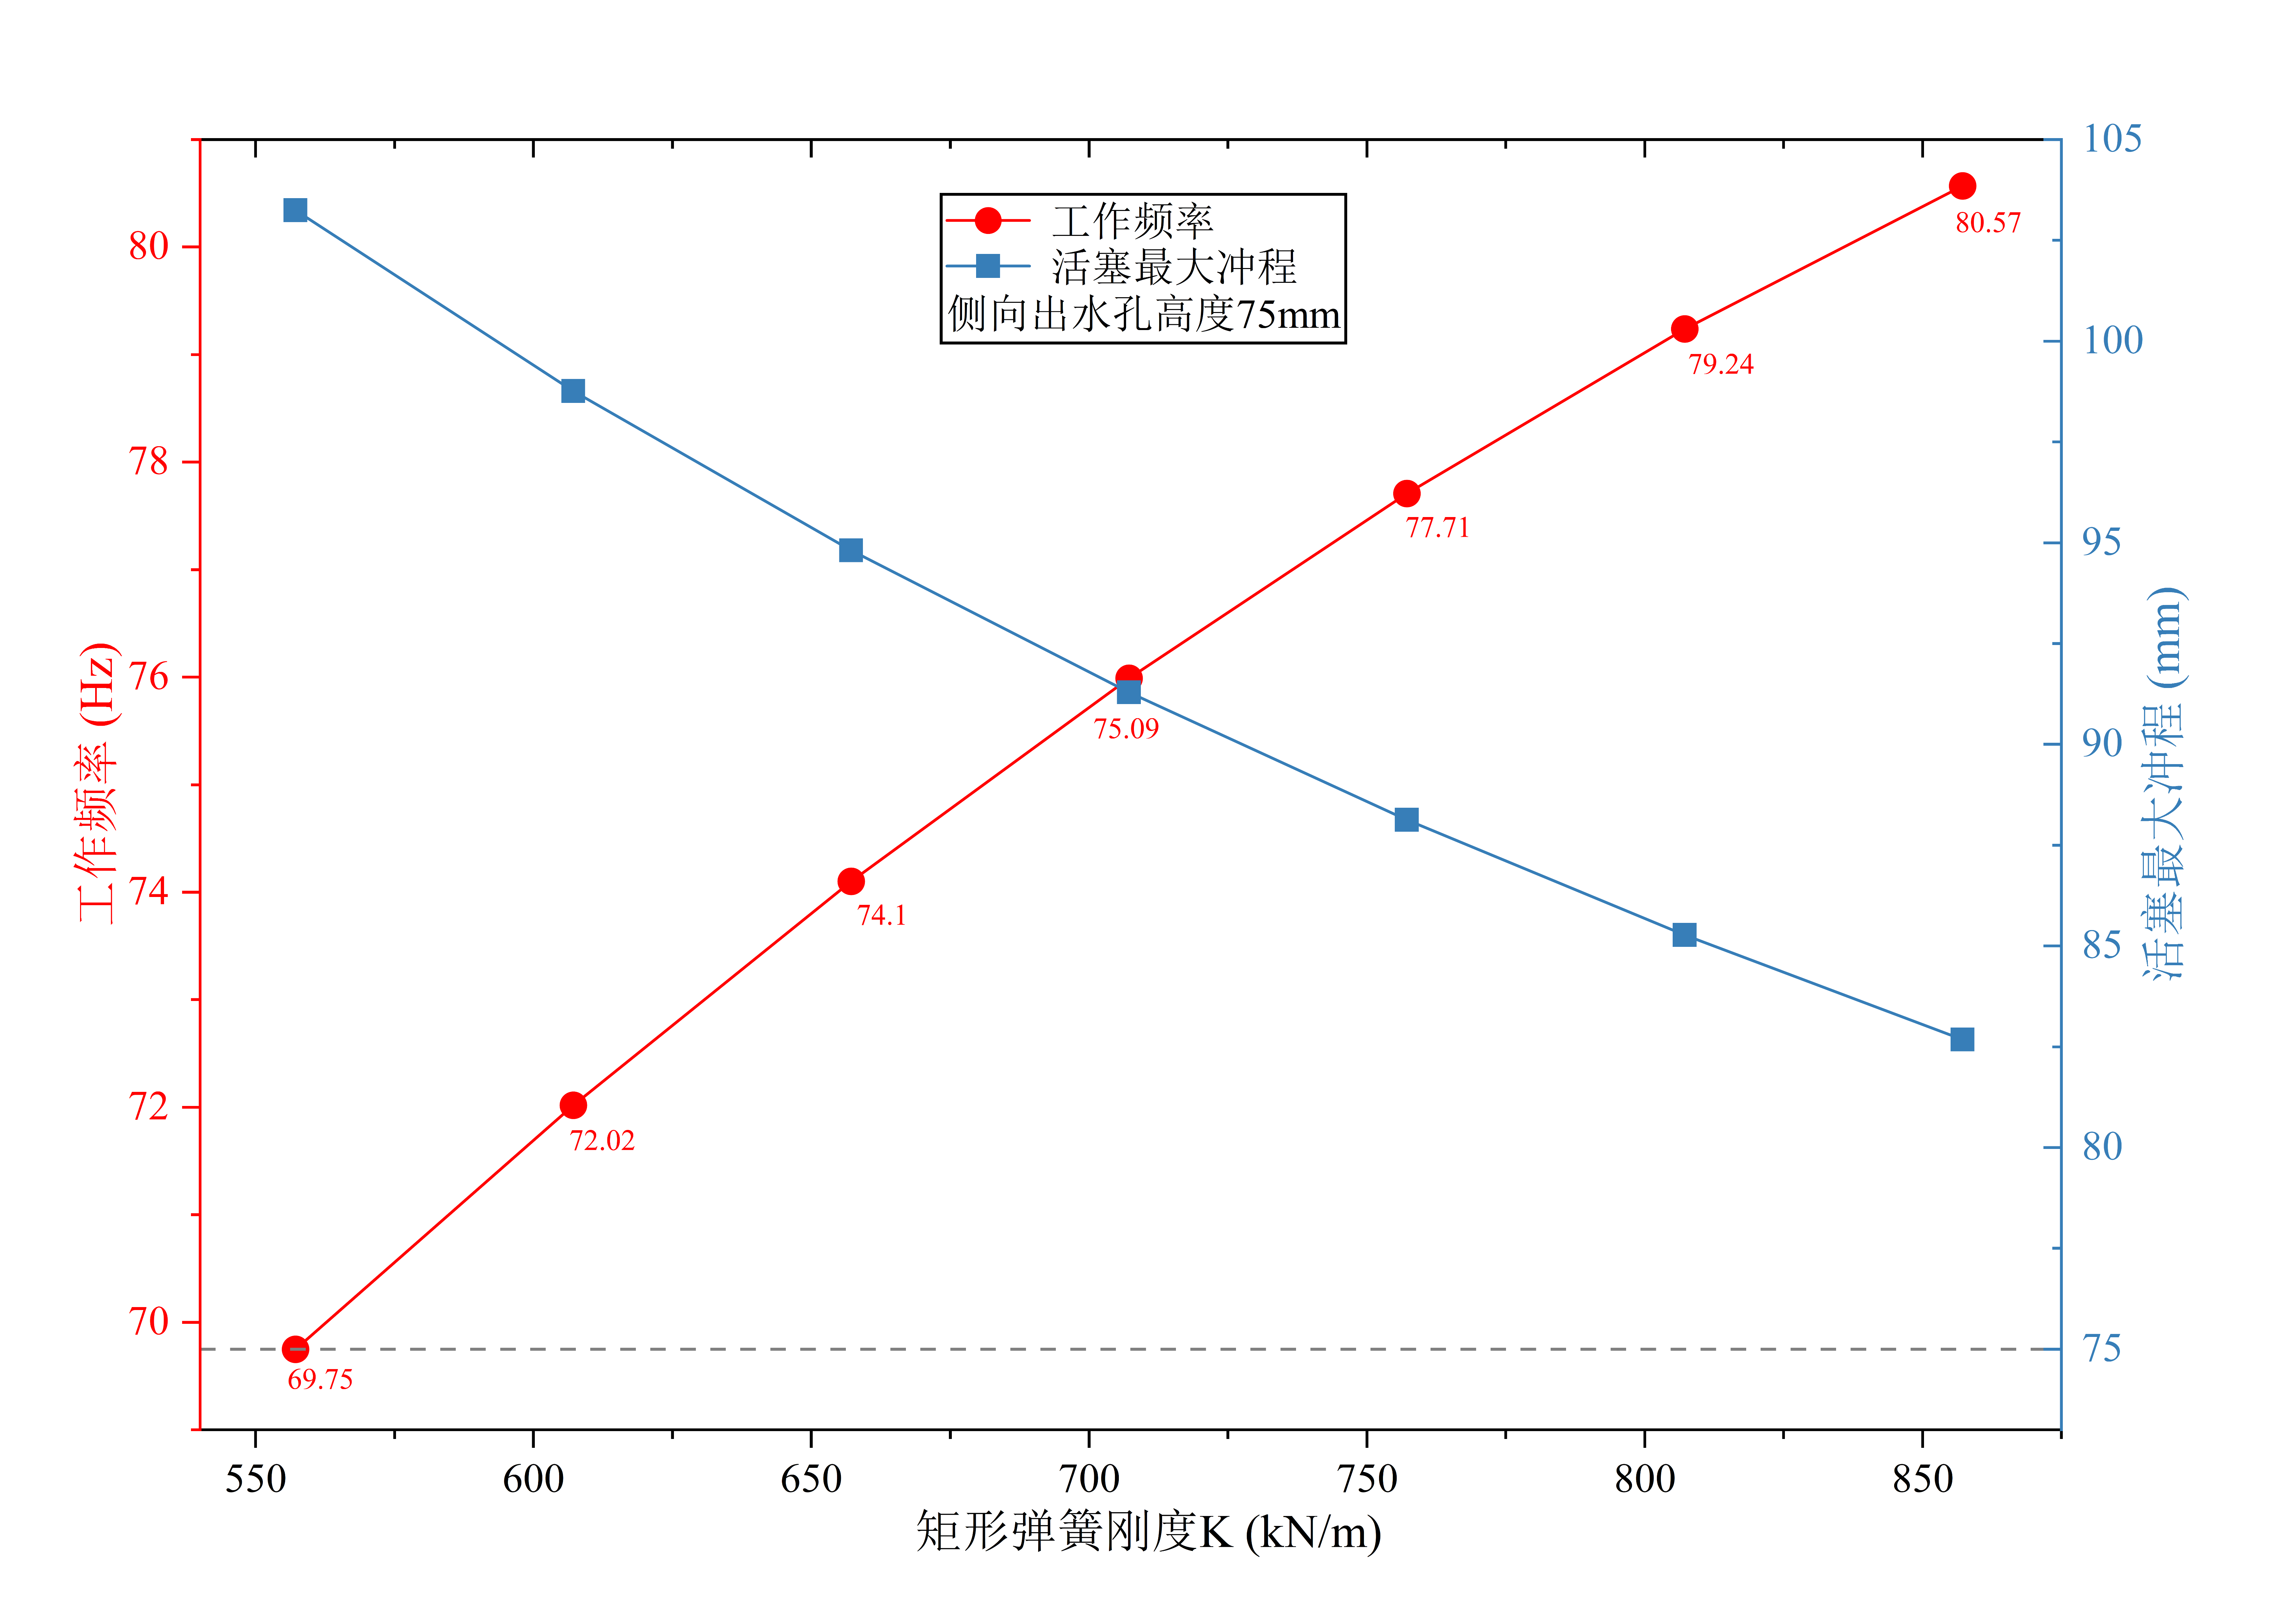
\includegraphics[width=0.7\textwidth]{figure/chapter3/pulse-module-frequency-stroke-VS-spring-K.png}
	\caption{脉冲发生模块弹簧刚度$K$与工作频率、冲程关系特征曲线}
	\label{fig:pulse_module_frequency_stroke_VS_spring_K}
\end{figure}

（3）侧向出水孔高度对脉冲发生模块频率的影响

侧向出水孔高度$h$是脉冲发生模块结构设计的关键参数，为揭示侧向出水孔高度 对系统动态特性的影响规律，本节在$h=65mm$至$90mm$的设计区间内，以$5mm$为梯度，绘制了活塞位移与速度随时间变化曲线对比图\ref{fig:piston_displacement_VS_h}。对比发现，随着$h$值的增大，活塞位移图像的波峰也随之升高，$h$值的增大也推迟了活塞越过侧向出水孔的时刻，使得蓄能阶段在整个周期中的占比增加。侧向出水孔下移不仅拉长了活塞到达最大冲程所需的时间，更因为冲程的加深，迫使活塞在复位时必须跨越更长的距离，因此活塞运动周期加长。如图\ref{fig:piston_velocity_VS_h}所示，随着$h$值的增大，活塞正向速度峰值变化不明显，这表明系统向下的综合加速度在位移小于$65mm$时便已归零并发生反转。因此，无论泄流孔是在$65mm$还是$90mm$处打开，活塞都已经提前达到正向最大速度。随着$h$值的增大，活塞正向速度波形变宽，代表着活塞维持在向下冲击状态的时间被拉长。观察活塞负向速度，随着$h$值的增大，活塞复位阶段的绝对负向速度越大。

\begin{figure}[htbp]
	\centering
	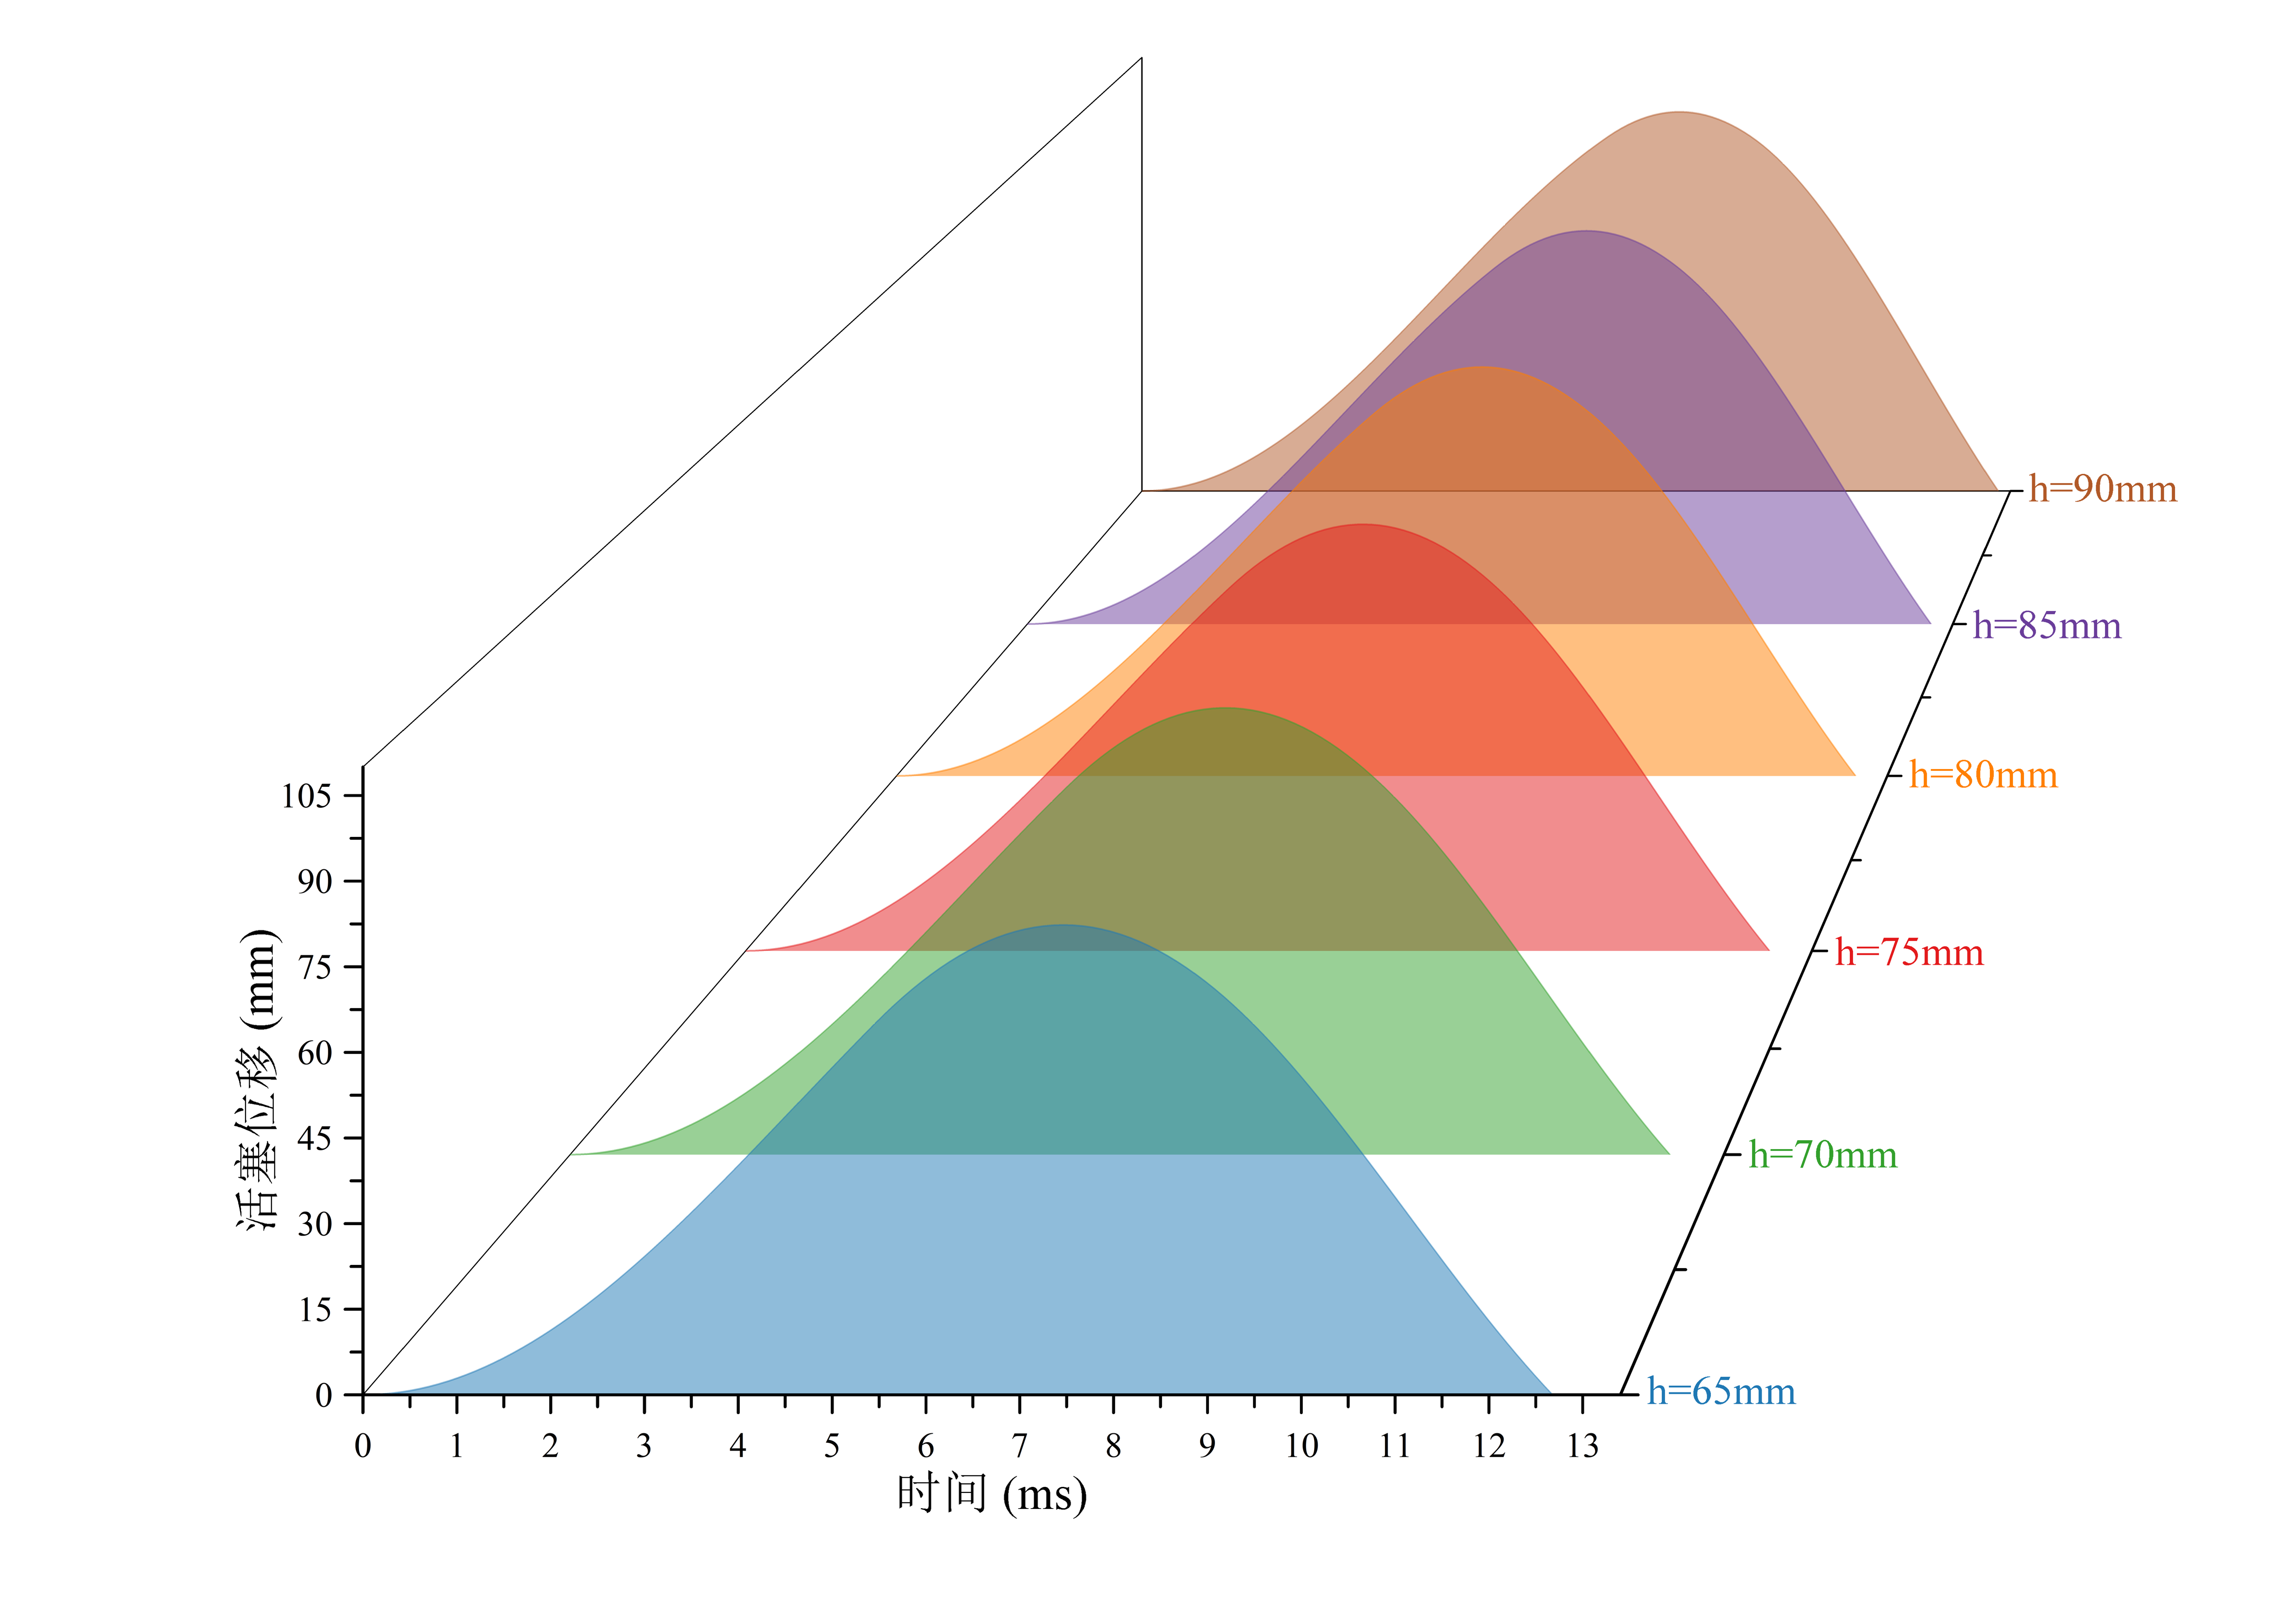
\includegraphics[width=0.7\textwidth]{figure/chapter3/piston-displacement-VS-h.png}
	\caption{活塞位移随侧向出水孔高度$h$变化曲线对比图}
	\label{fig:piston_displacement_VS_h}
\end{figure}

\begin{figure}[htbp]
	\centering
	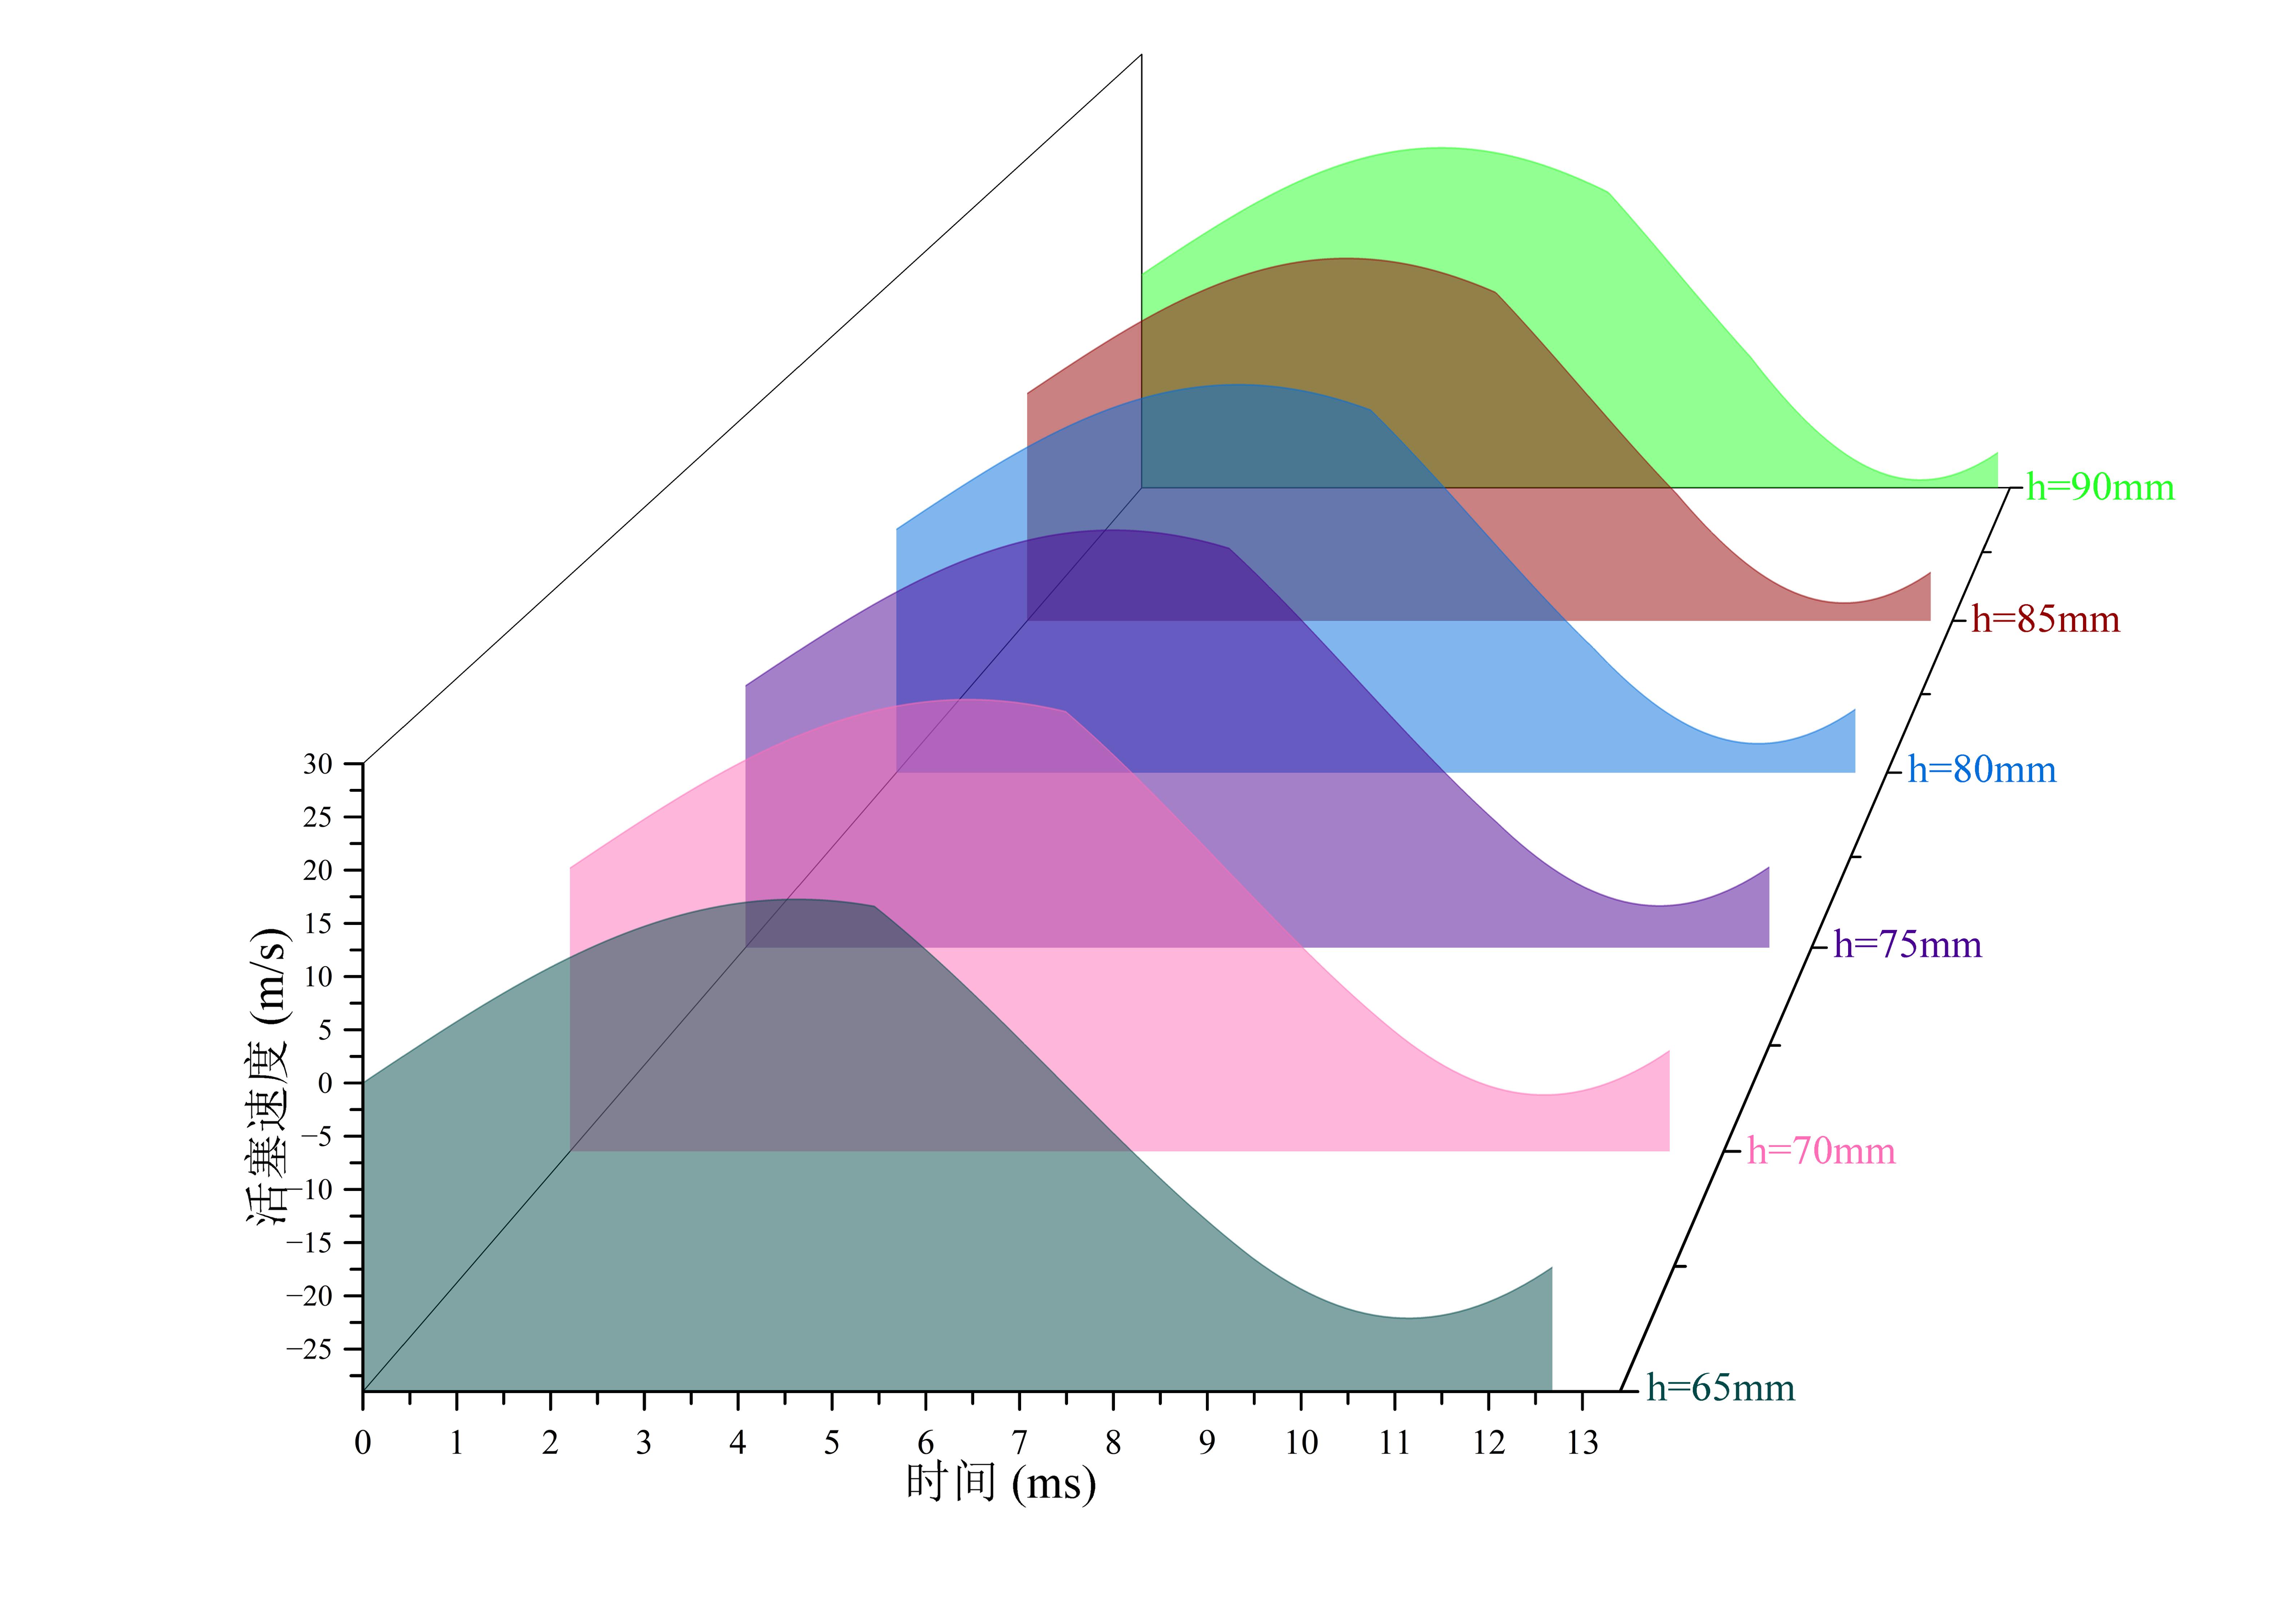
\includegraphics[width=0.7\textwidth]{figure/chapter3/piston-velocity-VS-h.png}
	\caption{活塞位移随侧向出水孔高度$h$变化曲线对比图}
	\label{fig:piston_velocity_VS_h}
\end{figure}


侧向出水孔高度对工作频率与冲程的影响特征曲线如图\ref{fig:piston_frequency_stroke_VS_h}所示，随着侧向出水孔高度$h$增大，活塞蓄能阶段距离延长，单次脉冲耗时拉长，脉冲发生模块工作频率减小。图中灰色虚点线代表了泄流孔的物理开启阈值，而蓝色实线代表活塞的最大位移距离。两者之间填充的浅蓝色阴影区域，即表征了活塞越过开孔位置后的开孔有效余量。随着侧向出水孔高度$h$增大，阴影区域的形态收缩，脉冲发生模块开孔有效余量减少，因此在设计脉冲发生模块时，应保证适宜的开孔有效余量，既要保证足够的脉冲频率，也要满足足够的活塞冲程。

\begin{figure}[htbp]
	\centering
	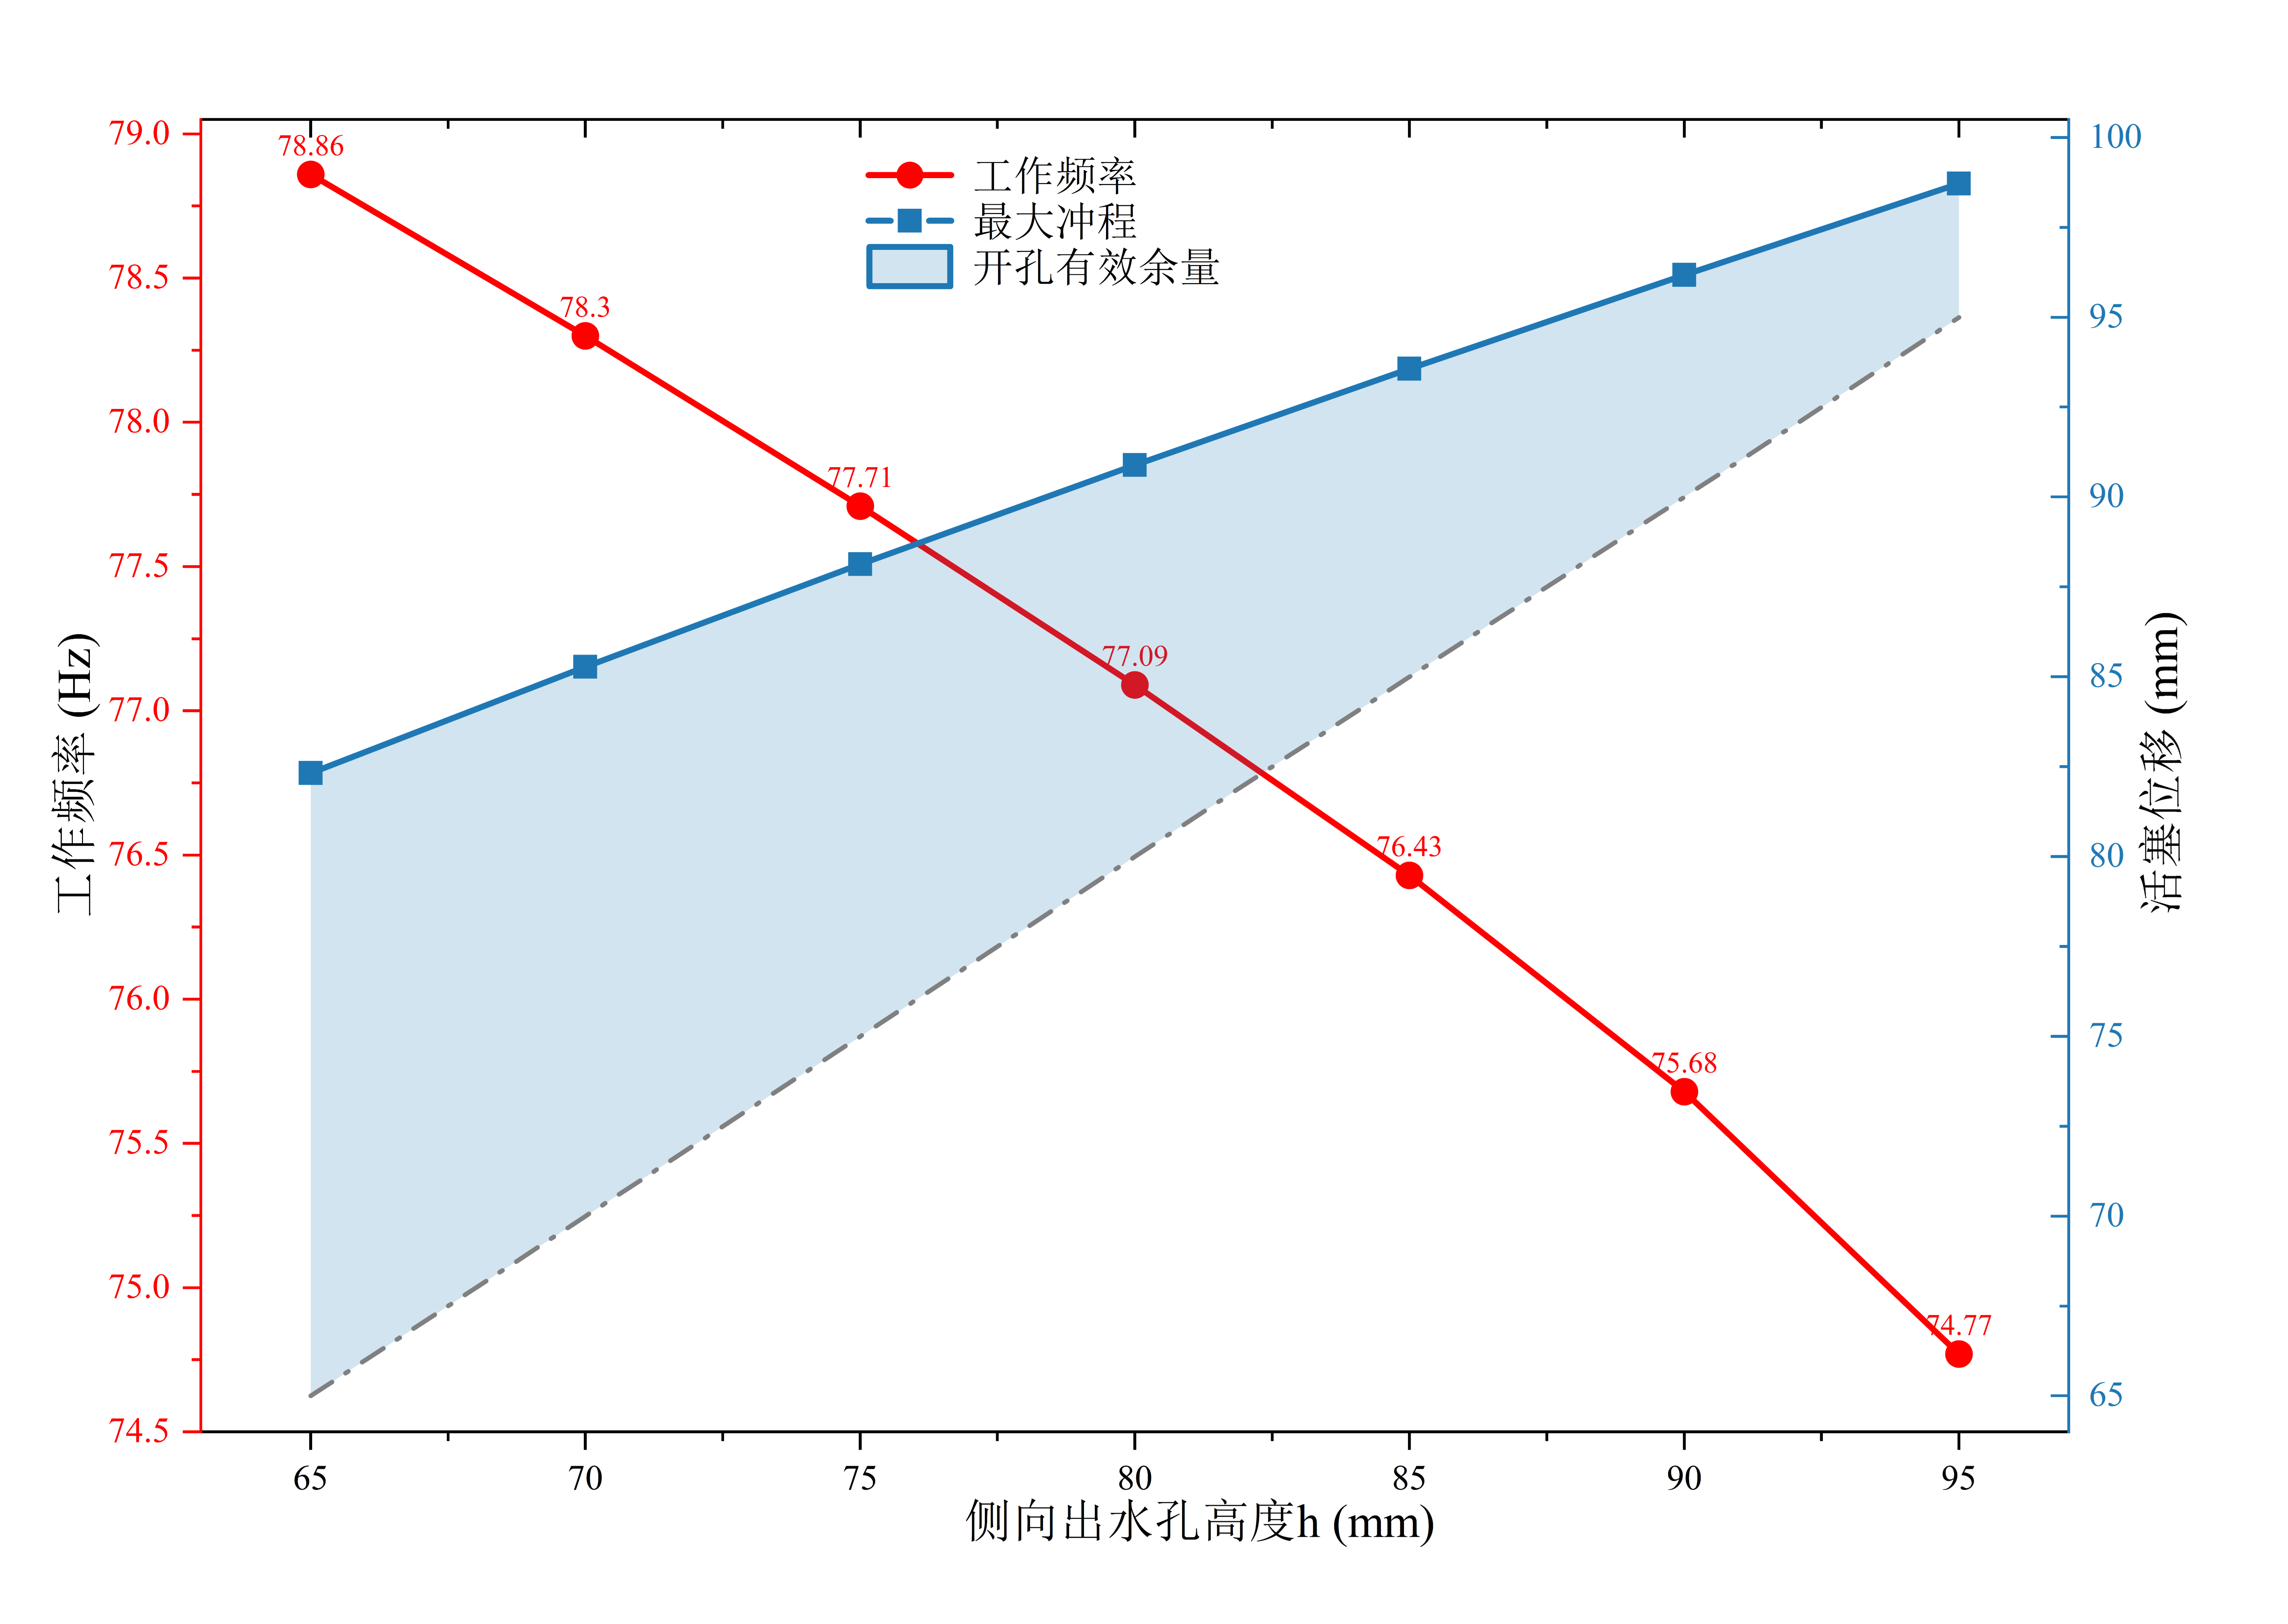
\includegraphics[width=0.7\textwidth]{figure/chapter3/piston-frequency-stroke-VS-h.png}
	\caption{侧向出水孔高度$h$对工作频率与冲程的影响特征曲线}
	\label{fig:piston_frequency_stroke_VS_h}
\end{figure}

\subsection{水力脉冲冲砂洗井工具下砂砾运移仿真分析}
在上一小节中，本文对脉冲冲砂洗井工具进行结构设计以及动力学特性进行研究，成功建立了脉冲发生模块的瞬态动力学数学模型，并深入研究了输入排量$Q$、工具矩形弹簧刚度$K$、工具侧向出水孔高度$h$等核心参数对系统频率与冲程的影响规律。

本小节通过FLUENT软件对使用脉冲冲砂洗井工具下环空井眼的清洁进行数值模拟，对比分析有无工具对环空内砂砾质量的影响，评估脉冲冲砂洗井工具冲砂洗井的效率优势。

\subsubsection{脉冲发生模块的网格划分与边界条件}
井筒内壁尺寸$244.475\mathrm{mm}$，钻杆尺寸$88.9\mathrm{mm}$，井筒长度$1.5\mathrm{m}$，在此基础上，对脉冲发生模块的井筒环空几何模型进行网格划分。如图\ref{fig:pulser_mesh}所示，总体使用poly-hexcore网格划分，网格总数105786，网格质量0.9。

\begin{figure}[htbp]
	\centering
	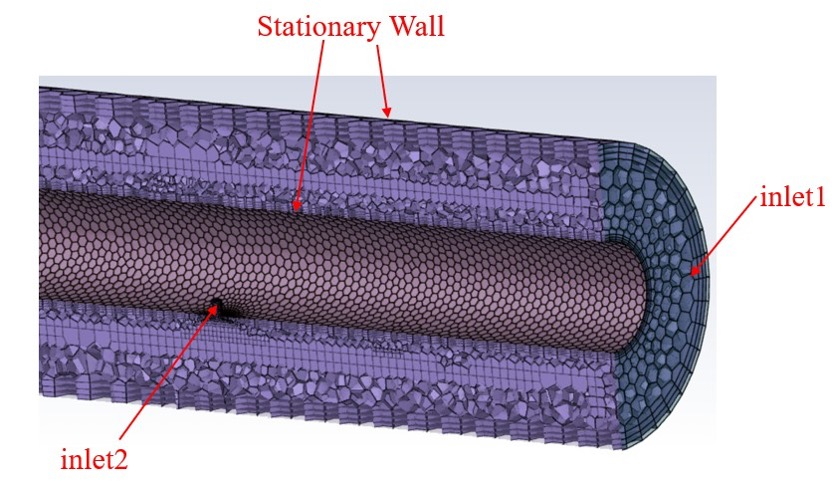
\includegraphics[width=0.7\textwidth]{figure/chapter3/pulser-mesh.jpg}
	\caption{使用水力脉冲冲砂洗井工具的网格划分}
	\label{fig:pulser_mesh}
\end{figure}

根据实际工况，数值模型的入口边界条件定义为冲砂液速度入口和砂砾的颗粒质量入口inlet1；喷嘴处的入口边界条件定义为冲砂液速度入口inlet2；出口的边界条件定义为压力出口outlet；井壁和钻杆内壁面的边界条件定义为固定无滑移的Stationary Wall，具体参数如表4.1所示：

%这里缺少表4.1

脉冲发生模块的侧向出水孔为直径$D=8\mathrm{mm}$的圆孔。设活塞在$t$时刻的位移为$x(t)$，基准开启高度$l_1=75\mathrm{mm}$，则圆孔的瞬时裸露高度$h(t)=\min(y(t)-l_1,D)$。根据微积分弓形面积公式，瞬时开孔面积$A_{\mathrm{out}}(t)$与瞬时射流速度$V_{\mathrm{out}}(t)$遵循以下耦合方程[70]：

%这里缺少公式4.29
其中，$V_p(t)$为活塞瞬时速度，$\mathrm{m/s}$。结合以上喷射时间和喷射速度，通过Fluent读取UDF文件产生周期性的脉冲射流。

\subsubsection{水力脉冲冲砂洗井工具对携砂效率的影响}
为了对比有无脉冲冲砂洗井工具对井筒除砂效率的影响，需设置一组无脉冲冲砂洗井工具的对照组仿真，其它参数保持一致。有脉冲冲砂洗井工具组喷嘴位于钻杆入口$0.4\mathrm{m}$处。通过Fluent欧拉多相流计算井筒内的砂砾质量随时间的变化规律，对比无脉冲洗井工具对照组的砂床运移效率。从图\ref{fig:sand_mass_in_annular_VS_time_pulser_rigid}可以看出，使用脉冲冲砂洗井工具的砂砾质量比无脉冲洗井工具对照组降低了19\%，该工具可以明显提升砂砾运移效率[71-72]。

\begin{figure}[htbp]
	\centering
	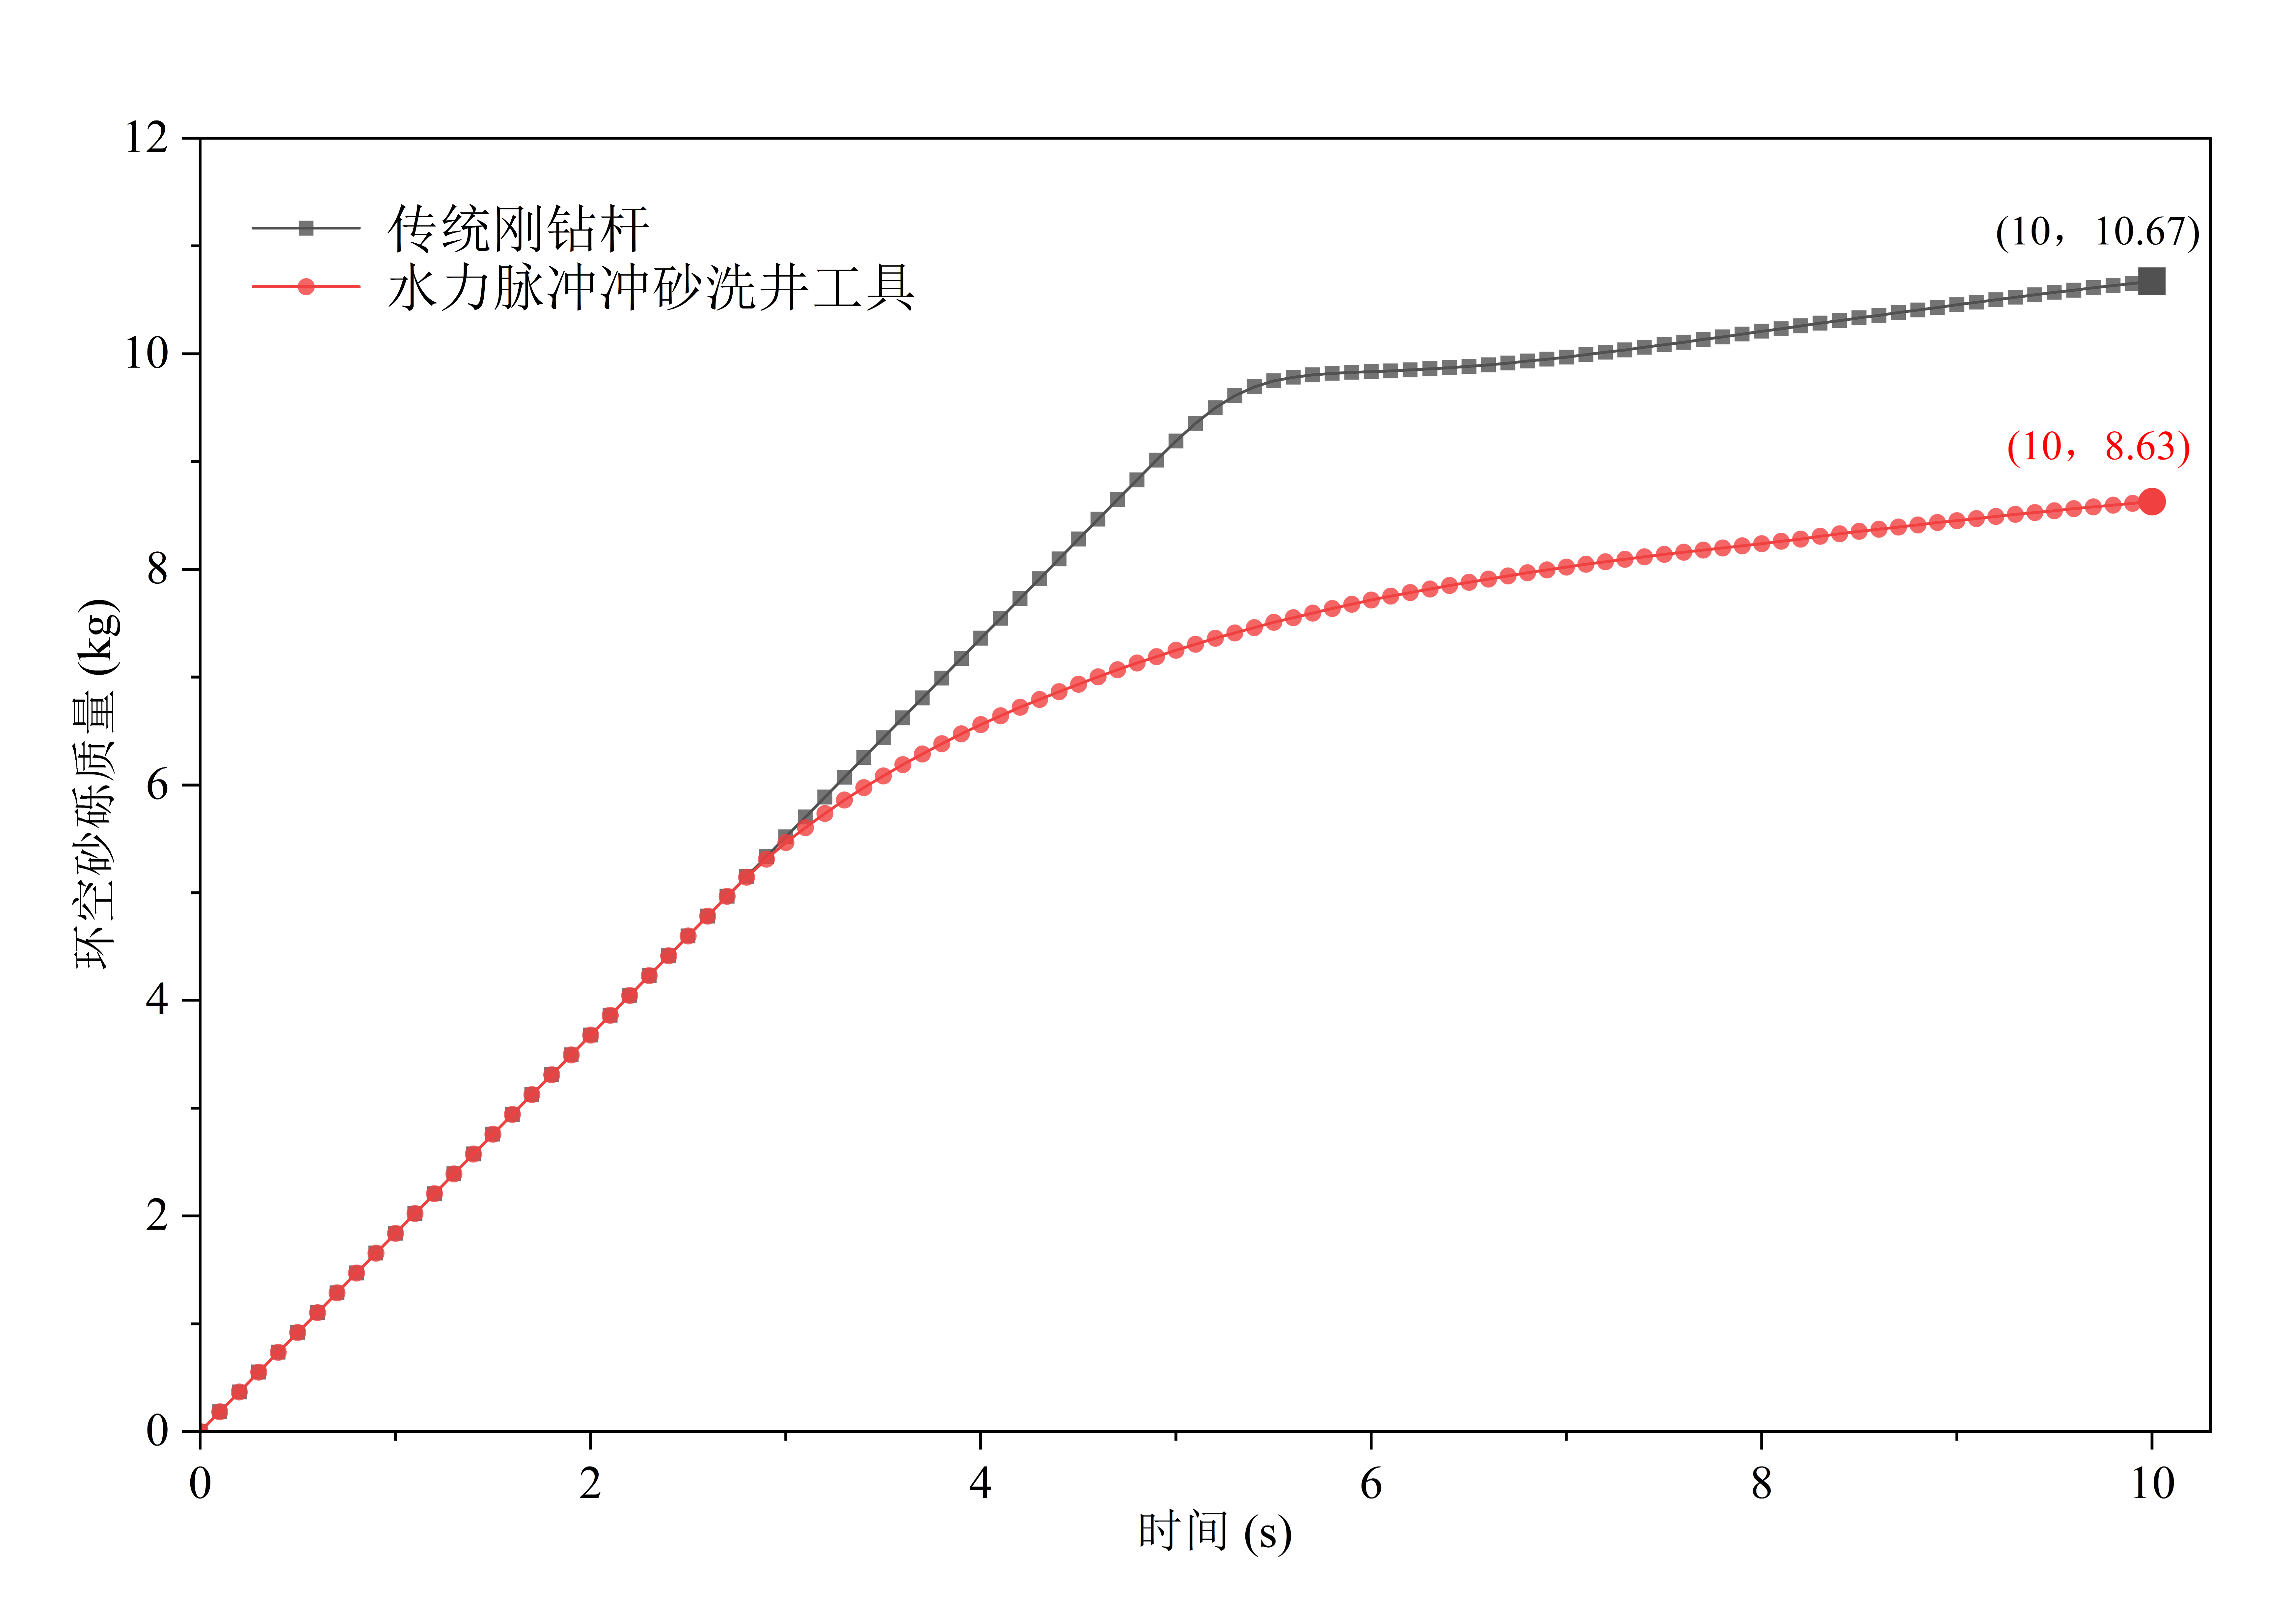
\includegraphics[width=0.7\textwidth]{figure/chapter3/sand-mass-in-annular-VS-time-pulser-rigid.png}
	\caption{环空砂砾质量变化对比图}
	\label{fig:sand_mass_in_annular_VS_time_pulser_rigid}
\end{figure}

图\ref{fig:axial_velocity_near_nozzle_section}为喷嘴截面处冲砂液轴向速度对比图，带有工具的截面环空下方冲砂液轴向速度明显高于传统刚钻杆环空下方的冲砂液轴向速度，这说明带有脉冲喷嘴的钻杆可以有效提高冲砂液的携砂能力，使砂砾的运移效率显著提高。
\begin{figure}[htbp]
	\centering
	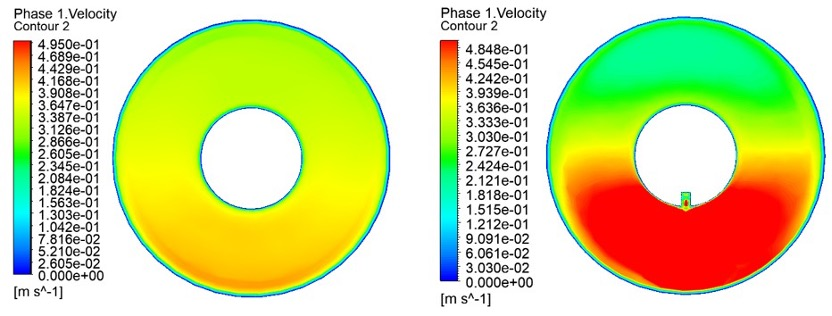
\includegraphics[width=0.7\textwidth]{figure/chapter3/axial-velocity-near-nozzle-section.jpg}
	\caption{喷嘴截面处冲砂液轴向流速对比图}
	\label{fig:axial_velocity_near_nozzle_section}
\end{figure}

图\ref{fig:sand_volume_at_nozzle_section}为相同时刻下喷嘴截面处有无工具砂砾体积分数对比图，从图中可以看出，使用传统刚钻杆仿真组的砂砾会在环空底部发生沉积，使用水力脉冲冲砂洗井工具仿真组的砂砾由于脉冲喷嘴的冲击压力并未沉积在环空底部，而是富集于环空两侧，富集区域最大体积分数远小于传统刚钻杆仿真组。

\begin{figure}[htbp]
	\centering
	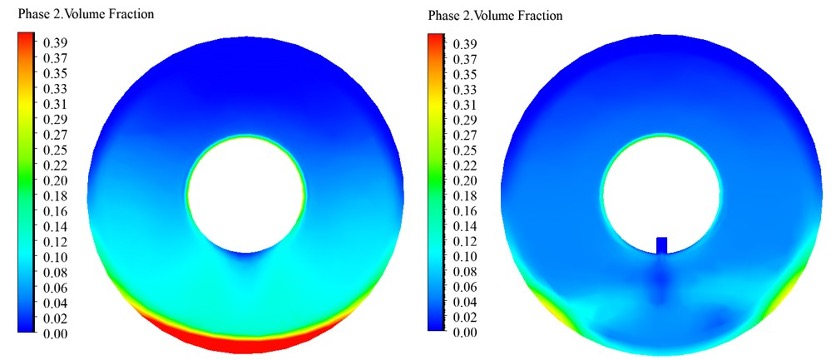
\includegraphics[width=0.7\textwidth]{figure/chapter3/sand-volume-at-nozzle-section.jpg}
	\caption{喷嘴截面处冲砂液轴向流速对比图}
	\label{fig:sand_volume_at_nozzle_section}
\end{figure}


图\ref{fig:sand_volume_at_verticle_section}为相同时刻下环空有无工具砂砾体积分数对比图，从图中可以看出，使用传统刚钻杆仿真组的砂砾从入口处进入环空后迅速在环空底部发生沉积，并形成连续砂床。砂床右端运移到距离入口0.8m处。使用水力脉冲冲砂洗井工具仿真组的砂砾从入口处进入环空并开始沉积，当砂砾运移到脉冲喷嘴处时会被脉冲喷嘴产生的冲击压力与负压抽吸效果重新卷积到井筒环空中，并在脉冲喷嘴下游处沉积，砂床右端已运移到压力出口。可以发现，使用工具可以有效抑制砂砾在工具处的沉积现象，并且显著提升砂床的运移效果。

\begin{figure}[htbp]
	\centering
	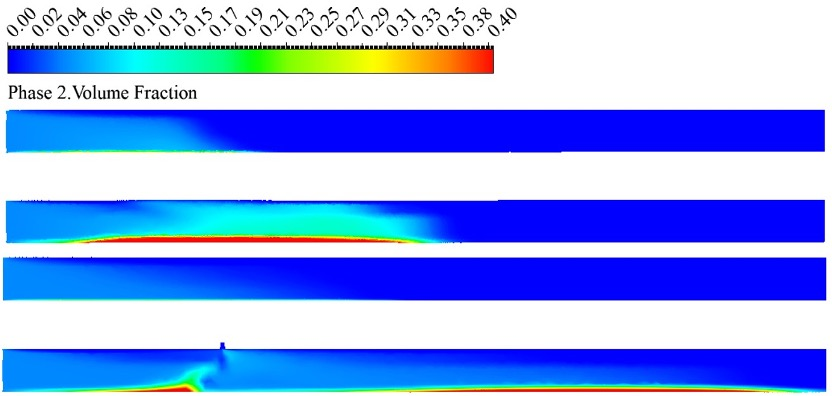
\includegraphics[width=0.7\textwidth]{figure/chapter3/sand-volume-at-verticle-section.jpg}
	\caption{喷嘴截面处冲砂液轴向流速对比图}
	\label{fig:sand_volume_at_verticle_section}
\end{figure}

\subsection{水力脉冲喷头流动仿真}
\subsubsection{水力脉冲计算域的构建与离散}

为了定量研究清洁工具产生的脉冲射流的清洁作用，需建立流动模型，采用流体动力学方法进行研究。在建立流动模型过程中，考虑到工具的外部表面平滑（如图3.1(a)所示），且水力脉冲对井筒的影响的窗口是喷嘴，为了研究脉冲频率的影响，依据隔离法的思想，可将研究对象选为喷嘴以外的环空区域，所构建的流体域如图\ref{fig:pulsing_nozzle_sub_model}(a)所示。
在网格划分采用多面体网格进行划分，能产生更多的邻居单元，能够更精确地计算控制体的梯度，在边界附近增加三层边界层以捕获准确的流动特征，提高计算准确度和精度。另外对流道差异转化较大的区域进行局部加密，优化网格质量，并进行网格无关性验证，最终的离散结果如图\ref{fig:pulsing_nozzle_sub_model}(b)所示。
\begin{figure}[htbp]
	\centering
	\subfloat[水力脉冲清洁工具流体域构建]{%
	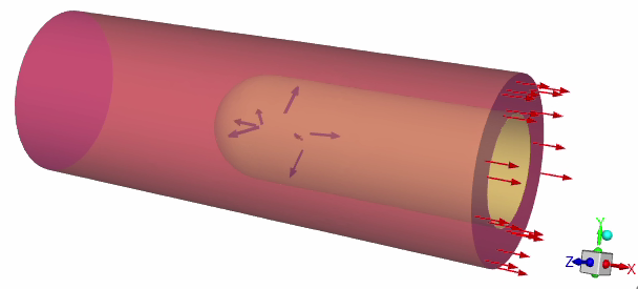
\includegraphics[width=0.45\textwidth]{figure/chapter3/nozzle-sub-fluid-domain.png}
	}
	%\vspace{1em}
	\subfloat[环空流体域的多面体离散结果]{%
	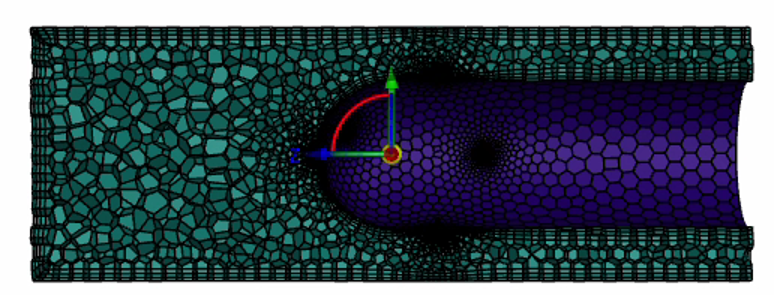
\includegraphics[width=0.45\textwidth]{figure/chapter3/nozzle-sub-fluid-domain-mesh.png}
	}
	\caption{水力脉冲喷头计算模型}
	\label{fig:pulsing_nozzle_sub_model}
\end{figure}


边界条件设置如下：出口假设为套管轴向内测，该设置对流场及仿真结果无影响，且避免了回流的影响，出口为压力出口，压力大小为大气压；入口边界条件设置为速度入口，该速度入口采取$25-45m^3/h$的动态范围脉动流量的转化量进行设置，该结构共设置7组喷嘴，每个喷嘴的尺寸直径为$\phi 3.25$，转化后的入口速度$v$为
\begin{equation}
	v=60.63 \sin⁡(2\pi/Tt)+262.73
\end{equation}

为研究脉动频率对压力的作用情况和井筒的清洁效果分别开展以下三组实验：$T=0.5s$、$1.0s$或$2.0s$。仿真采用的瞬态流动求解器，时间步长$0.001s$，初始流场的速度和压力置零。

\subsubsection{仿真结果及讨论}

为正确反应该水力脉冲清洁工具的清理能力，以冲击点的压力波动为因变量进行分析，$t=0.5s$时套管内壁面的压力分布如图\ref{fig:sress_distribution_at_case}所示。图\ref{fig:case_wall_pressure_t_dot5s}显示流体冲击作用对应下的近壁面压力最高，压力呈圆周状进行削减。图\ref{fig:case_wall_shear_t_dot5s}说明高速射流在壁面附近形成强烈的速度梯度，圆孔射流冲击壁面后形成径向流动，剪切应力由流体在壁面附近的黏性摩擦产生。剪切应力沿径向分布，能够扩大清洗覆盖范围，这种应力会克服污染物与管壁之间的黏附力，从而剥离附着物。高速射流带动周围流体形成涡流，使得流道内湍流强度较高，其瞬时脉动会增强剪切力的波动性，更有效地破坏污染物的结构，使剥离的污垢颗粒被卷吸进入主流，防止重新沉积。

\begin{figure}[htbp]
	\centering
	\subfloat[正压力]{%
	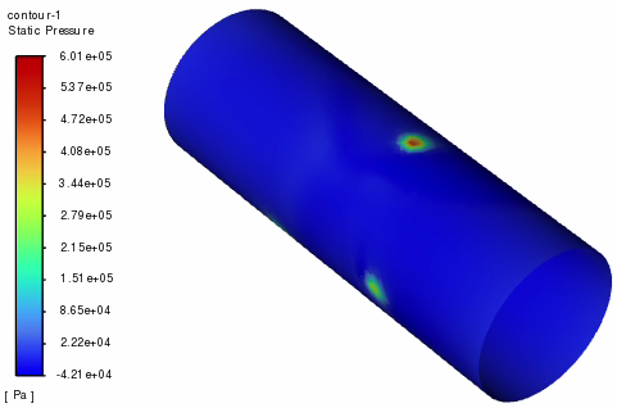
\includegraphics[width=0.45\textwidth]{figure/chapter3/case-wall-pressure-t-dot5s.png}
	\label{fig:case_wall_pressure_t_dot5s}
	}
	\vspace{1em}
	\subfloat[剪切应力分布]{%
	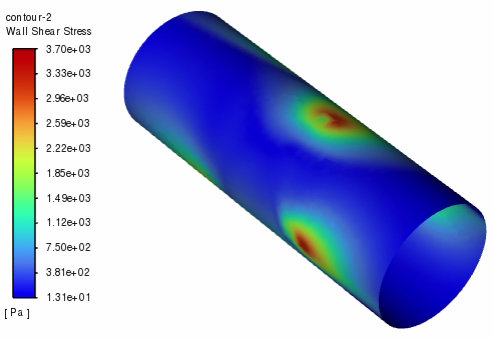
\includegraphics[width=0.45\textwidth]{figure/chapter3/case-wall-shear-t-dot5s.png}	\label{fig:case_wall_shear_t_dot5s}
	}
	\caption{水力脉冲喷头作用下套管内壁压力分布（$t=0.5s$）}
	\label{fig:sress_distribution_at_case}
\end{figure}

整个过程中，冲击压力与剪切应力协同起作用。射流的冲击压力首先使污染物破裂或松动，后续产生的持续的剪切应力将已松动的污染物卷吸进入流体主流，并随流道被带走，达到清洁壁面的目的。流体在流道内的速度流线图如图\ref{fig:nozzle_streamline_dot5s}所示。该图显示喷嘴孔射流流速逐渐减小，动压增大，并逐渐转化为静压作用于油管壁面或清理面，射流压力是影响清垢效率的一个重要因素，在其它条件不变的情况下,随着压力的增加，清垢效率明显提高。该过程通过压力变化反应了水力脉冲清洁工具的清理能力。同时由于射流方向与出口的关系，流场出现许多绕流，该绕流能从各个方向上作用于结垢物上，提升清理能力。

\begin{figure}[htbp]
	\centering
	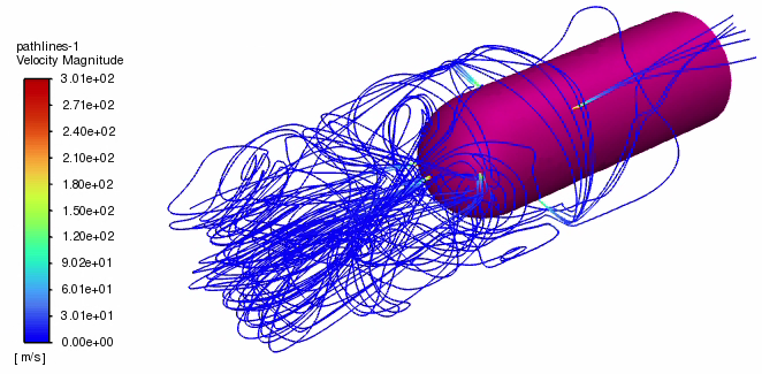
\includegraphics[width=0.7\textwidth]{figure/chapter3/nozzle-streamline-dot5s.png}
	\caption{喷嘴处速度流线图}
	\label{fig:nozzle_streamline_dot5s}
\end{figure}

为研究水力脉冲与压力脉动的关系，将图3.5显示的压力最高点设置为监测点，也就是每个喷嘴作用于井筒的直线冲击点作为监测点，共设置如图\ref{fig:monitoring_point_configuration}所示的6个监测点。当$T=0.5s$、$1.0s$和$2.0s$时，6个监测点对应的壁面压力随时间变化如图\ref{fig:monitoring_points_pressure_T_dot5s}至\ref{fig:monitoring_points_pressure_T_2s}所示。

\begin{figure}[htbp]
    \centering
    % 子图 (a)
    \subfloat[监测点设置]{%
        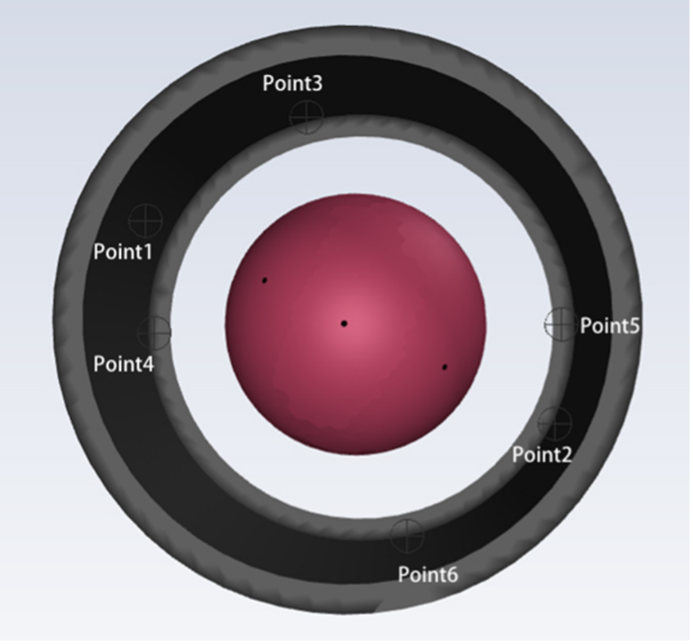
\includegraphics[width=0.4\linewidth]{figure/chapter3/monitoring-point-configuration.png}%
        \label{fig:monitoring_point_configuration}
    }
    % 子图 (b)
    \subfloat[$T=0.5s$]{%
        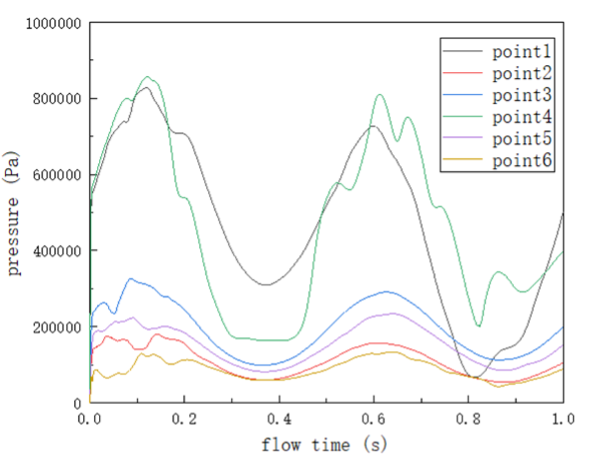
\includegraphics[width=0.45\linewidth]{figure/chapter3/monitoring-points-pressure-T-dot5s.png}%
        \label{fig:monitoring_points_pressure_T_dot5s}
    }
    \vspace{1em}
     % 子图 (c)
    \subfloat[$T=1.0s$]{%
        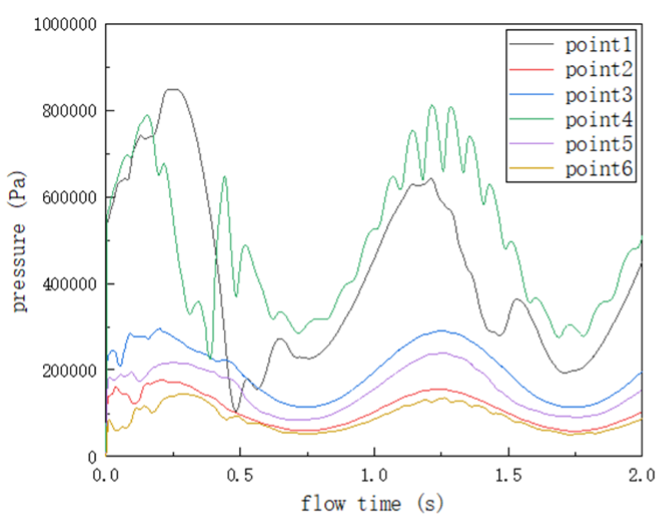
\includegraphics[width=0.45\linewidth]{figure/chapter3/monitoring-points-pressure-T-1s.png}%
        \label{fig:monitoring_points_pressure_T_1s}
    }
    % 子图 (d)
    \subfloat[$T=2.0s$]{%
        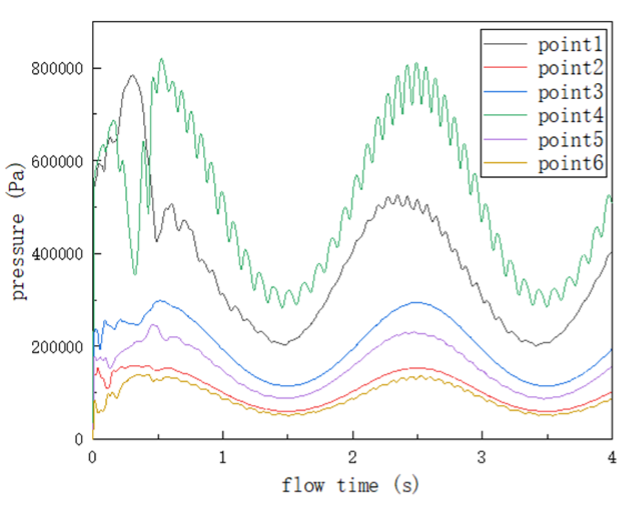
\includegraphics[width=0.45\linewidth]{figure/chapter3/monitoring-points-pressure-T-2s.png}%
        \label{fig:monitoring_points_pressure_T_2s}
    }
        \caption{套管壁面压力点监测结果}
    \label{fig:pressure_at_monitoring_points}
\end{figure}

图\ref{fig:monitoring_points_pressure_T_2s}显示某些监测点的压力较大，压力波动范围更大。由于安装的喷嘴角度不同，若喷嘴射流方向垂直于油管内壁，冲击点会形成驻点（流速降为零，动压转化为静压），导致局部压力显著升高。若射流与壁面存在夹角，高速射流会诱导剪切层分离，形成涡旋结构，这些涡周期性脱落会引发壁面压力剧烈波动，尤其在分离区再附着点附近。另外，由于存在多个射流，射流流场混合导致局部流速增加和压力梯度增强。油管圆柱曲率会改变射流发展路径，凸面曲率可能加速流动分离，进一步加剧压力波动。

随着周期的增加，总体作用点的压力波动幅值于相位保持一致，系统非线性（如边界层分离、射流-壁面相互作用、流道内反射播传播）可能将低频能量传递至高频，生成$4\omega$，$6\omega$等谐波，表现为小幅高频振荡。低频脉动使射流产生间歇性高压冲击，类似于“锤击”效应，适用于硬质或粘附性强的污垢，污垢在反复的低频压力加载下发生微裂纹扩展，最终整体剥离。高频压力波动诱发空化气泡，溃灭时产生局部微射流，直接冲击污垢微结构。高频脉动提升湍流强度（湍动能增加），使剪切应力分布更均匀。另外，观测到部分点高频流速下峰峰值更大，这主要是能量更易耗散，反射叠加效应较弱。

因此，在处理污垢时，压力波动产生的低频和高频成分共同作用，低频脉动剥离大块污垢，高频成分清除残留微粒。叠加高低频脉动，可同时实现宏观剥离和微观清洁。所以实际应用中需根据污垢特性（硬度、厚度、黏附性）调整脉冲频谱，必要时采用复合频率策略以兼顾清洗效率与精度。本章在进行入口脉冲频率选择时需同时考虑压力脉动的组合特性，叠加高低频脉动，以发挥最大的清洁能力。
本章针对连续砂床或严重出砂井况，常规水力冲砂冲砂效率低，除砂效果差的问题，提出并设计了一种新型水力脉冲冲砂洗井工具，能够有效破坏砂床表面并且抑制环空砂砾的再沉积，并对工具进行以下研究：

（1）设计了由旋转喷头模块与脉冲发生模块协同工作的新型水力脉冲冲砂洗井工具。阐述了旋转模块利用偏心射流反冲力矩实现360°冲洗，以及脉冲模块利用往复活塞与弹簧机构将稳态泵注液转化为高频压力脉冲波的工作原理。

（2）对脉冲发生模块进行动力学建模，针对工具内部流体压力与机械部件的耦合机制，基于连续性方程与牛顿运动定律，建立包含蓄能、开启、喷射与复位四个阶段的非线性常微分方程组。通过求解该模型，定量考察了输入排量、矩形弹簧刚度及侧向出水孔高度对活塞冲程与系统工作频率的影响规律，为工具关键物理参数的优选提供数学计算依据。

（3）最后利用Fluent软件模拟脉冲射流动态冲刷下井底沉积砂床的剥离与运移过程，通过对比使用该工具前后的环空携砂质量与流场分布特征，结果显示，使用水力脉冲冲砂洗井工具能够显著提升砂砾的运移效率，实现有效清砂。
	% !TeX root = ../../main.tex
\section{拆装步骤及操作方式}
\subsection{脉冲器拆装步骤及操作方式}
1）下井前准备

(1) 了解井况，确定套管或者管径规格和深度等基本信息；

(2) 确定工具活动部件是否连接稳固，外观是否存在不合格如裂纹缺口问题，如出现，则不能入井；

(3) 确定工具和其余钻具的连接扣型是否正确；

(4) 可按照推荐排量在井台上检验工具是否能正常振动，喷水口严禁对人。

2）操作方法

(1) 核准下井油管尺寸；

(2) 用“通井规”通井、洗井，若和其他具有通、洗井功能的工具配合使用时可一体化完成；

(3) 将工具缓慢下至设计位置；

(4) 连接管线等地面加压设备后试压；

(5) 开泵加压、冲洗井底，推荐的排量为100L/min-500L/min（直至上返水无污物止）；

(6) 控制出口流量，加大井口压力、排量到设计压力、排量进行正常振动作业；

(7) 每振动1小时，停振10分钟，累计振动作业4-6小时停振、泄压、将工具取出。

3）注意事项

(1) 工具与管柱的连接扣必须拧紧。

(2) 公扣端需要朝下。

(3) 脉冲器在下入过程中如遇阻，应慢慢旋转几圈后再下放。

(4) 不能连续振动超过十分钟。

\subsection{旋转喷头拆装步骤及操作方式}

\subsubsection{拆卸}

准备工具：3mm + 4mm内六方扳手、3/8\inch 套筒、套筒扳手、卸扣工装、可调扳手、链钳\footnote{注：重要！工具需夹紧在装配钳台上。}

\begin{itemize}
	\item 取出筒体2上螺钉
	
	\begin{figure}[htbp]
		\centering
		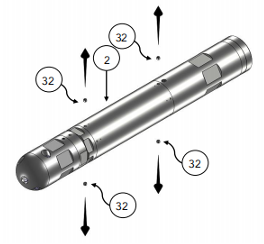
\includegraphics[width=0.5\textwidth]{figure/chapter3/part1-3in1/nozzle-unsetup-step1.png}
		%\caption{拆卸步骤1：取出筒体2上螺钉}
		\label{fig:unscrew_from_body2}
	\end{figure}	
 
		\item 从筒体2上卸掉上接头1和波簧15
\begin{figure}[htbp]
	\centering
	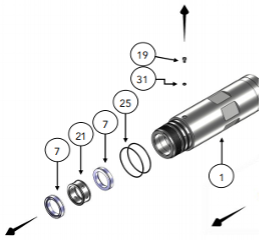
\includegraphics[width=0.5\textwidth]{figure/chapter3/part1-3in1/nozzle-unsetup-step2.png}
	%\caption{拆卸步骤2：卸掉上接头1和波簧15}
	%\label{fig:unscrew_from_body2}
\end{figure}
 
		\item 从上接头1上取出骨架油封7，密封垫环21，卸掉带孔螺钉19取出O型圈31。
\begin{figure}[htbp]
	\centering
	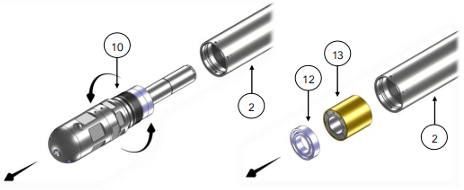
\includegraphics[width=0.7\textwidth]{figure/chapter3/part1-3in1/nozzle-unsetup-step3.png}
	%\caption{拆卸步骤3：取出骨架油封7、密封垫环21与O型圈31}
	%\label{fig:unscrew_from_body2}
\end{figure}
 
		\item 从本体2上卸掉底部帽，取下轴承12和隔套13。
	\begin{figure}[htbp]
		\centering
		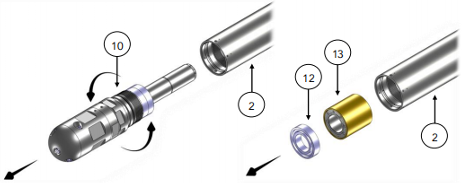
\includegraphics[width=0.7\textwidth]{figure/chapter3/part1-3in1/nozzle-unsetup-step4.png}
		%\caption{拆卸步骤4：卸掉底部帽，取下轴承12和隔套13}
		%\label{fig:unscrew_from_body2}
	\end{figure}
	
	\item 先从旋转头16上卸掉紧定螺钉34，然后将旋转头16从喷头连接体10上卸下来。然后再将紧定螺钉33从喷头连接体10上卸下来，最后将喷头连接体10从芯轴4上卸下来。
	\begin{figure}[htbp]
		\centering
		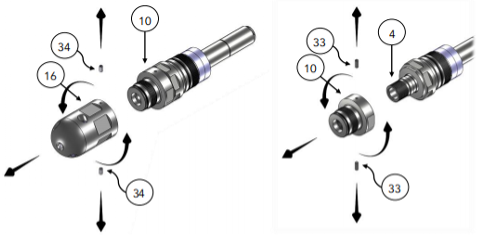
\includegraphics[width=0.7\textwidth]{figure/chapter3/part1-3in1/nozzle-unsetup-step5.png}
		%\caption{拆卸步骤5：卸下旋转头16与喷头连接体10}
		%\label{fig:unscrew_from_body2}
	\end{figure}
	
 
	\item 从芯轴4上卸掉底部帽8和轴承12，插入座3和O型圈26。
	\begin{figure}[htbp]
		\centering
		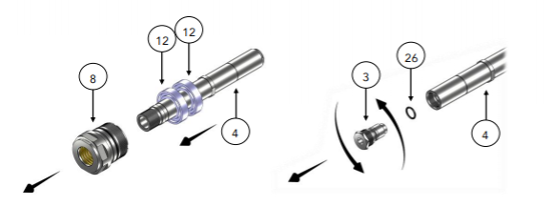
\includegraphics[width=0.7\textwidth]{figure/chapter3/part1-3in1/nozzle-unsetup-step6.png}
		%\caption{拆卸步骤6：卸掉底部帽8和轴承12，取出插入座3与O型圈26}
		%\label{fig:unscrew_from_body2}
	\end{figure}
	
 
	\item 从底部帽8上卸掉平衡活塞座9，取出大弹簧20和O型圈28，取出平衡活塞6。
	\begin{figure}[htbp]
		\centering
		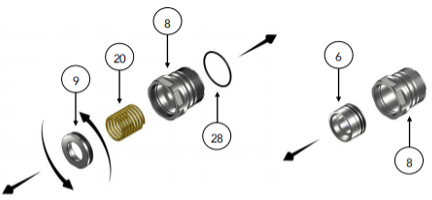
\includegraphics[width=0.7\textwidth]{figure/chapter3/part1-3in1/nozzle-unsetup-step7.png}
		%\caption{拆卸步骤7：卸掉平衡活塞座9，取出大弹簧20、O型圈28与平衡活塞6}
		%\label{fig:unscrew_from_body2}
	\end{figure}
 
	\item 从喷头连接体10上取出O型圈29和30。从平衡活塞上取出骨架油封7和O型圈27。
		\begin{figure}[htbp]
		\centering
		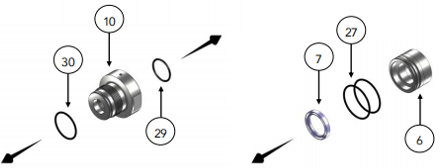
\includegraphics[width=0.7\textwidth]{figure/chapter3/part1-3in1/nozzle-unsetup-step8.png}
		%\caption{拆卸步骤8：取出O型圈29、30与骨架油封7}
		%\label{fig:unscrew_from_body2}
	\end{figure}
 
	\item 从旋转喷头16上取下喷嘴18，从隔套13上取出连通隔套5。
	\begin{figure}[htbp]
		\centering
		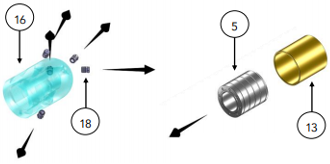
\includegraphics[width=0.7\textwidth]{figure/chapter3/part1-3in1/nozzle-unsetup-step9.png}
		%\caption{拆卸步骤9：取下喷嘴18与连通隔套5}
		%\label{fig:unscrew_from_body2}
	\end{figure}
	
\item 	准备清洗和检测。
	
\end{itemize}
	
\subsubsection{装配}
准备工具：3mm+4mm内六方扳手、3/8\inch 套筒、套筒扳手、扣工装、可调扳手、链钳\footnote{注：重要！工具需夹紧在装配钳台上。}。装配前，检查所有部件是否磨损和腐蚀；润滑所有密封区域并安装O型圈/支撑环。涂抹润滑脂润滑所有螺纹防止粘扣。
\begin{itemize}
	\item 在喷头连接体10上安装O型圈29和O型圈30，在平衡活塞6上安装骨架油封7和O型圈27。
	
	\item 在旋转喷头16上安装喷嘴和引流体17。
	
	\item 在底部帽8上安装O型圈28并依次装入已经小装好的平衡活塞6和大弹簧20和平衡活塞座9。
	
	\item 在芯轴4上安装O型圈26和插入座3，掉头将两件轴承12装入芯轴4并将底部帽8和芯轴连接到位。
	
	\item 将小装好的喷头连接体10和小装好的芯轴4连接到位，并将紧定螺钉33安装在喷头连接体10上。然后将小装好的旋转喷头16和喷头连接体10连接到位后，将紧定螺钉34安装在旋转喷头上。
	
	\item 将底部帽8和筒体2连接到位，在筒体上安装紧定螺钉32，将连通隔套5和隔套13安装，依次将小装后的隔套13、轴承12、波簧15装入筒体2。确保连通隔套5和芯轴4的限位台阶抵紧。
	
	\item 在上接头1上安装O型圈25，O型圈31和带孔螺钉19，并依次在上接头1上装入骨架油封7和密封垫环21。
	
	\item 将装好的上接头1和小装好的筒体2连接到位后安装紧定螺钉32。
	
	\item 安装好之后注油进行旋转测试。
\end{itemize}
	
	
\subsubsection{注油}

准备工具：3mm + 4mm内六方扳手、可调扳手、链钳\footnote{
注（重要）：工具需夹紧在装配钳台上。}

\begin{itemize}

	\item 从筒体2上取掉紧定螺钉32，然后将上接头1从筒体2上卸下来。
	\item 保持旋转喷嘴直立，使用混合硅胶油-1000，直到油位位于筒体2的槽螺孔下方。
 
注：建议让喷嘴直立过夜，使油沉淀。回装喷嘴时，可能需要补注摩擦螺钉下方的油。

	\item 将上接头1和筒体2连接至0.31\inch（7.87 mm），卸掉带孔螺钉19继续上扣至紧扣扭矩。
	
	\item 在筒体2上安装好带孔螺钉19和紧定螺钉32。
 
	\item 安装喷嘴后准备测试。
	\end{itemize}
	
\subsubsection{功能测试}
\begin{itemize}
	
	\item 充油后目视检查工具，检查在修整过程中是否有泄漏或任何密封件损坏。
	
	\item 用手旋转工具，确保其转动平稳，不过度用力，不干涉。
	
	\item 将工具连接到泵上，并开始以最低速率循环通过泵，逐渐增加速率，直到它开始旋转并记录流量。
	
	\item 继续观察恒定流速下是否出现泄漏情况，如果观察到任何泄漏，请参考总装图，以确定哪个密封/密封正在通过。应注意，该工具存在内置的泄漏路径，允许流体通过外壳离开工具。
	
	\item 通常，所有尺寸的工具都会开始以小于0.6次/分的速度旋转，具体值可能存在差异，这取决于芯轴上新唇密封的实际配合状态。如果启动旋转所需的流量高于预期，建议增加流量5$\sim$10 L/min；当新唇密封磨损后，应停止泵送并重复上述操作。
	
	\item 如果不能以所需的流量启动旋转，建议将驱动旋转的两个90度喷嘴更换成更大孔径的喷嘴，以允许喷嘴的流量比例更大。
	\end{itemize}
	
\subsubsection{操作方法}
	\begin{itemize}
		
	\item 该工具可以单独用于清洗油套管，也可以和其他工具组合作业。
	
	\item 将旋转头下入井内距离清洁位置1$\sim$3 m处，开泵循环，排量建议为100 L/min，逐渐加大流量但最大不应超过300 L/min。同时若配置其他工具，需要保持稳定的循环，平稳地上下活动钻具。
	
	\item 起钻时要求平稳、低速、严禁剧烈振动与撞击。
	\end{itemize}

\subsection{液压刮管器拆装步骤及操作方式}

\subsubsection{下井前准备}
		\begin{itemize}
		\item 了解井况，确定套管规格和深度等基本信息；
		\item 根据刮管工艺要求，确定套管是否需要液压启动后再进行刮管。
		\end{itemize}
	
\subsubsection{操作方法}
\begin{itemize}
	\item 下井前按作业要求依次连接好管柱，刮管器前端需接与套管规格对应的扶正器；推荐管柱组合：通井钻头+扶正器+液压刮管器+上部钻柱；
	\item 接上刮管器后，夹紧下接头，用大钳咬住上接头，拧紧刮管器各连接螺纹；
	\item 需要进行刮管作业时，将刮管器下入到所需的井深位置后，投入钢球，开泵进行打压启动作业；其中，刮管器打开压力$=$静液柱压力$+$泵压（绝对压力），即泵压$\ge$绝对压力$-$静液柱压力；
	\item 观察泵压有下降后，说明刮管器启动，此时通过上提、下放工具，如此反复进行刮管作业；
	\item 刮管作业中观察指重表无任何显示，即下放悬重不降、上提悬重不升，表明已刮削干净；
	\item 若上提过程中多次遇阻仍无法上提，可投入复位钢球，开泵将刮刀体强行收回；
	\end{itemize}
\subsubsection{注意事项}
	\begin{itemize}
		\item 工具与管柱的连接扣必须拧紧。
		\item 刮管器在下井过程中如遇阻，应慢慢旋转几圈后再下放。
		\item 刮削过程中，必须始终保持循环畅通。
	\end{itemize}
\subsection{毛刷刮管器拆装步骤及操作方式}
\subsubsection{拆卸}\label{sec:unstep_swiper}
	\begin{itemize}
	\item 去掉防掉螺钉后，用拧扣机拆卸下接头；
	\item 依次取出芯轴上的上扶正套、毛刷体、下扶正套、剪切套、剪切定位套；
	\item 取出所有O型圈与销钉。
	\item 零部件清洗，打磨处理工具表面锈蚀部分；
	\item 清洗并晾干所有零部件。
	\end{itemize}
\subsubsection{装配}
按照\ref{sec:unstep_swiper}所述“拆卸”步骤的反序组装各部件。注意：
\begin{itemize}
	\item 所有密封圈及工具配合面涂润滑油，上扶正套、毛刷体、下扶正套、剪切套、剪切定位套与芯轴间涂抹黄油；
	\item 产品连接螺纹涂钻具螺纹脂；
	\item 上、下接头的上扣扭矩为$10\ \mathrm{kN\cdot m}$；
	\item 产品本体喷涂天蓝色脂肪族面漆，毛刷喷银色漆；
	\item 两端接头螺纹涂防蚀脂并佩戴护丝。
	\end{itemize}
\subsubsection{使用方法}
\begin{itemize}
	\item 	根据井眼尺寸选择合适的套管刮管器。
	\item MSQ型套管刮管器用钻柱送入井底进行刮管作业，情况允许也可以用钢丝绳或者连续油管送入。
\end{itemize}
\subsubsection{操作方法}
\begin{itemize}
	\item 	该工具可以与液压刮管器以及强磁打捞器配合使用，也可以在刮完井之后使用。
	\item 	将MSQ型套管刮管器下到井底离通井位置3$\sim$5 m处，开泵循环。将MSQ型套管刮管器在该位置上下活动，保持循环的情况下平稳地上提钻柱。
	\item 	起钻时要求平稳、低速、严禁剧烈振动与撞击。
\end{itemize}

\section{维护与保养}
\begin{itemize}
	\item 	出井后应清洗干净，并检查各零件。如弹簧失效必须更换。各螺纹涂螺纹脂，各零件涂油，置于阴凉干燥处保存。
\item 	 每次作业后，都应将工具完全拆开并清洗，更换所有O形圈和损坏的弹簧，检查脉冲器上连接螺纹是否有松、退扣的情况发生。用肉眼检查所有密封面和接头丝扣是否损坏，若发现有损坏的零件应予更换，否则会对工具的可靠性产生不利影响。
\item 	在拆卸、保养前，应准备好正确、有效的装配图和工具保养维护说明书及工具维护保养单。
\item 	对高温井的作业和有酸及硫化氢存在的修井作业，应提前更换相应耐腐蚀耐高温密封件和配件。
\end{itemize}


















\chapter{“四合一”通刮刷磁集成式井筒清洁工具设计}
	\subsection{工具总体结构设计}
“四合一”通刮刷磁集成式井筒清洁工具\footnote{下文简称为“四合一工具”}是一种集机械刮削、刷洗清扫与强磁吸附功能于一体的井筒清洁装备。该工具主要用于清除套管内壁的水泥残留、铁屑、毛刺、石蜡及油污等沉积物，以满足新井射孔前的井筒净化要求，并为封隔器等密封工具提供合格的座封环境。同时，针对长期服役油井出现的套管内壁缩径、破裂及毛刺等损伤，该工具可辅助进行井筒内径检测与管壁修复。

工具的结构如图\ref{fig:structure_4_in_1}缩式，采用长轴式布局，主要由上接头、心轴系统、连接套、刮刀模块、毛刷模块、磁吸清理模块及辅助定位机构组成。各功能单元沿轴向依次排布，通过模块化连接方式实现组合，使工具兼具结构简洁性与操作灵活性。心轴作为核心承载部件，承担轴向推力、旋转载荷及各功能模块产生的反作用力，并确保各模块在工作过程中保持同轴状态。刮刀模块与毛刷模块可根据实际作业需求选装组合，以适应不同井况的清洁要求。

该工具的作业机制上是通过机械切削、挤压破碎与辅助清扫的协同作用实现套管内壁硬垢的高效清除。工作时，工具在外部驱动力作用下沿套管轴向运动，心轴将动力传递至各功能模块。刮刀模块中，安装于刀架上的齿形刮刀在弹簧预紧力作用下始终保持与管壁的贴合状态；当刀齿尖端接触硬垢层时，产生较大的局部接触应力，对垢层进行压入与剪切，促使硬垢内部萌生裂纹并逐步扩展，最终导致垢层破碎与剥离。采用弹簧浮动加载结构后，刀片可根据垢层厚度与管壁形态变化自动调节伸缩量，在维持稳定切削压力的同时避免刚性冲击对刀具造成的损伤。在刮削作业完成后，后方毛刷模块对破碎后残留的细小颗粒进行清扫，进一步提升管壁清洁度；磁吸模块则对清理过程中产生的铁磁性碎屑进行有效吸附，防止其再次沉积。此外，工具心轴上设置有扭曲弹簧部件，当刮刀遇到顽固坚硬杂物时可被压缩储能，通过障碍后释放能量以起到缓冲保护作用。通过刮削、刷洗与磁吸的多级协同，该工具能够实现对套管内壁硬垢的高效、彻底清除。

对应的工具规格分别为7\inch 、9-5/8\inch 和13-3/8\inch。提交了三种型号的工具设计图纸。


\begin{figure}[htbp]
	\centering
	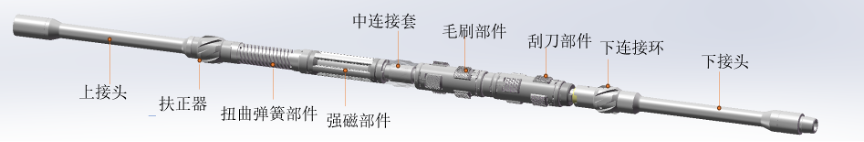
\includegraphics[width=1.\textwidth]{figure/chapter3/structure-4-in-1.png}
	\caption{四合一工具总体结构}
	\label{fig:structure_4_in_1}
\end{figure}

\begin{table}[htbp]
\centering
\caption{四合一工具技术参数}
\label{tab:zkg_params}
\begin{tabular}{cccccccccc} % 10列：型号、总长、水眼、套管磅级PPF、扶正体外径、刮刀外径范围、本体外径、接头扣、抗拉/抗扭强度
\toprule
规格 & \begin{tabular}[c]{@{}c@{}}总长\\ (mm)\end{tabular} & \begin{tabular}[c]{@{}c@{}}水眼\\ (mm)\end{tabular} & \begin{tabular}[c]{@{}c@{}}套管磅级\\ PPF\end{tabular} & \begin{tabular}[c]{@{}c@{}}扶正体\\ 外径\\ (mm)\end{tabular} & \begin{tabular}[c]{@{}c@{}}刮刀外径\\ (mm)\end{tabular} & \begin{tabular}[c]{@{}c@{}}本体外径\\ (mm)\end{tabular} & \begin{tabular}[c]{@{}c@{}}接头扣\\ (API)\end{tabular}& \begin{tabular}[c]{@{}c@{}}抗拉\\ (kN)\end{tabular} & \begin{tabular}[c]{@{}c@{}}抗扭\\（$\mathrm{kN\cdot m}$）\end{tabular} \\
\midrule
\multirow{4}{*}{7\inch} & \multirow{4}{*}{6500} & \multirow{4}{*}{40} & 17$\sim$20 & 158.24 & 159.77$\sim$171.96 & \multirow{4}{*}{139.7} & \multirow{4}{*}{NC38} & \multirow{4}{*}{1600} & \multirow{4}{*}{20} \\
& & & 20$\sim$26 & 155.58 & 155.70$\sim$167.89 & & & & \\
& & & 26$\sim$32 & 151.38 & 151.13$\sim$163.32 & & & & \\
& & & 32$\sim$35 & 146.05 & 146.56$\sim$158.75 & & & & \\
\midrule
\multirow{3}{*}{9-5/8\inch} & \multirow{3}{*}{6492} & \multirow{3}{*}{57.15} & 29.3$\sim$32.3 & 222.25 & 224.28$\sim$245.62 & \multirow{3}{*}{203.2} & \multirow{3}{*}{NC50} & \multirow{3}{*}{4000} & \multirow{3}{*}{50} \\
& & & 36$\sim$53.5 & 213 & 212.09$\sim$233.68 & & & & \\
& & & 47$\sim$59.4 & 209 & 209.04$\sim$230.38 & & & & \\
\midrule
\multirow{2}{*}{13-3/8\inch} & \multirow{2}{*}{6512} & \multirow{2}{*}{71.4} & 54.5$\sim$72 & 308 & 306.83$\sim$328.17 & \multirow{2}{*}{285.75} & \multirow{2}{*}{\begin{tabular}[c]{@{}c@{}}6-5/8\\ REG\end{tabular}} & \multirow{2}{*}{7800} & \multirow{2}{*}{110} \\
& & & 77$\sim$92 & 301.63 & 298.96$\sim$320.29 & & & & \\
\bottomrule
\end{tabular}
\end{table}

%对表中的数值进行说明：
%套管磅级：套管单位长度的重量，PPF：Pounds Per Foot（磅每英尺）

\subsubsection{四合一工具主要功能部件}

四合一工具主要功能部件如图\ref{fig:main_function_unite_4_in_1}所示。

刮刀模块（\ref{fig:mechanism_scratcher_4_in_1}）是工具完成硬垢破碎的核心部件，主要包括刀架、固定环、固定销、挡块、弹簧以及可更换齿形刀片。刀片安装于刀架槽内，在弹簧作用下能够产生径向浮动位移，使刀片能够适应套管内壁尺寸变化。当工具进入套管后，刀片受到管壁限制并保持与内壁接触。
        工具运动过程中，刀片齿尖首先接触硬垢层，通过较小接触面积形成较高局部压力，使垢层产生压裂和剪切破坏。当应力超过硬垢强度后，裂纹扩展并导致垢层剥离。
        
   毛刷模块(\ref{fig:mechanism_swiper_4_in_1})安装于刮刀模块后方，主要用于清除刮削后的残余垢屑。毛刷块同样采用浮动安装方式，可以根据套管内壁变化自动调整接触状态。在刮刀完成硬垢破碎后，毛刷通过柔性接触将附着的小颗粒和残余沉积物清除，提高最终清洁效果，降低碎屑重新附着的可能性。
   
   强磁部件（\ref{fig:mechanism_mag_sub_4_in_1}）通过固定销分别于两侧的挡环配合。主要作用是回收清洁过程中产生的磁性碎物。部分金属腐蚀产物和铁屑无法通过循环液及时排出，容易重新沉积于套管内部。强磁模块利用磁场吸附作用，将铁磁性颗粒吸附在工具表面，并随工具一起带出，实现井筒净化。
   
   扭曲弹簧（\ref{fig:mechanism_torsional_spring_4_in_1}）左端通过定位止转键，与左侧的扶正器的卡槽实现插接配合。右端以同样的方式与中挡环配合。工具中的扭曲弹簧部件不仅起到弹性支撑作用，还具有缓冲和保护功能。正常工作时，弹簧使刮刀片和毛刷块保持一定径向压力，保证其持续接触套管内壁。当遇到较坚硬或突出的杂物时，弹簧被压缩并储存能量，避免冲击载荷直接传递至工具连接部位；通过障碍后，弹簧释放能量，使刀片恢复工作位置，如图\ref{fig:flexible_scratch_system_4_in_1}所示。该结构提高了工具通过性和清洁稳定性，同时降低刀具损坏风险。
        
\begin{figure}[htbp]
    \centering
    % 子图 (a)
    \subfloat[刮刀部件结构]{%
        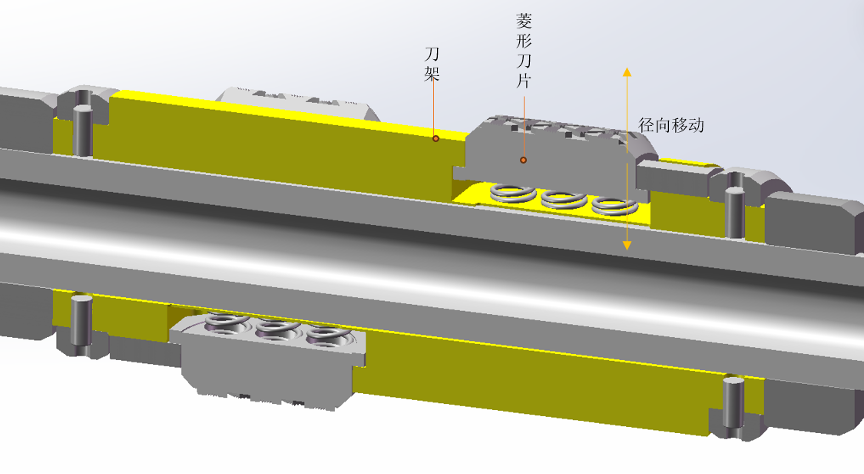
\includegraphics[width=0.45\linewidth]{figure/chapter3/mechanism-scratcher-4-in-1.png}%
        \label{fig:mechanism_scratcher_4_in_1}
    }
    \hfill
    % 子图 (b)
    \subfloat[毛刷部件结构]{%
        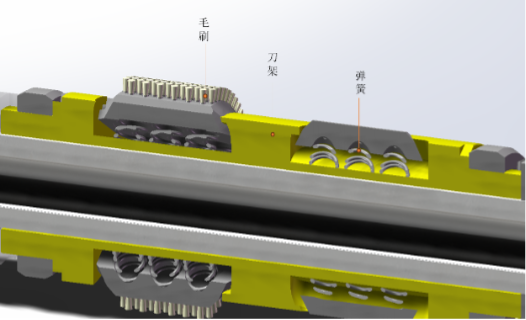
\includegraphics[width=0.45\linewidth]{figure/chapter3/mechanism-swiper-4-in-1.png}%
        \label{fig:mechanism_swiper_4_in_1}%
    }
    \vspace{1em}
      % 子图 (c)
    \subfloat[强磁部件结构]{%
        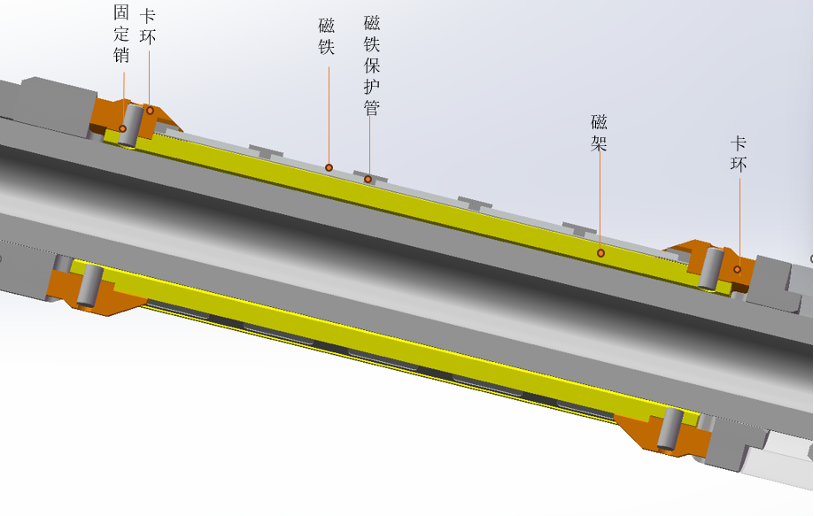
\includegraphics[width=0.45\linewidth]{figure/chapter3/mechanism-mag-sub-4-in-1.png}%
        \label{fig:mechanism_mag_sub_4_in_1}%
    }
    % 子图 (d)
    \subfloat[扭曲弹簧部件结构]{%
        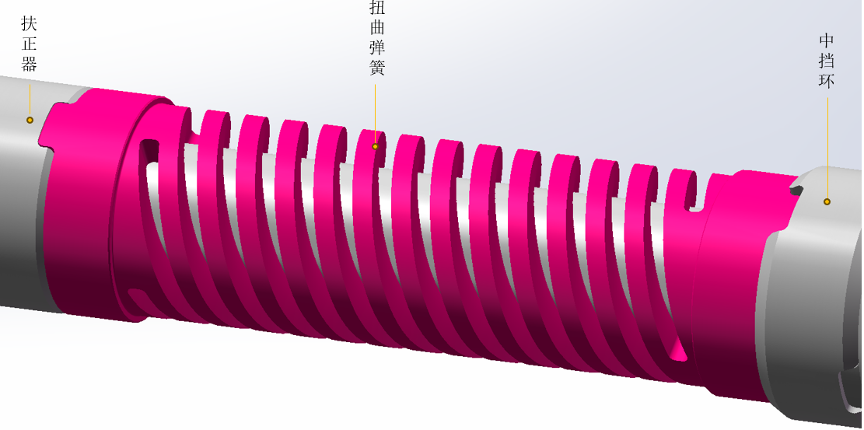
\includegraphics[width=0.45\linewidth]{figure/chapter3/mechanism-torsional-spring-4-in-1.png}%
      \label{fig:mechanism_torsional_spring_4_in_1}%
    }
    \caption{四合一工具主要功能单元}
        \label{fig:main_function_unite_4_in_1}
\end{figure}
      
\begin{figure}[htbp]
	\centering
	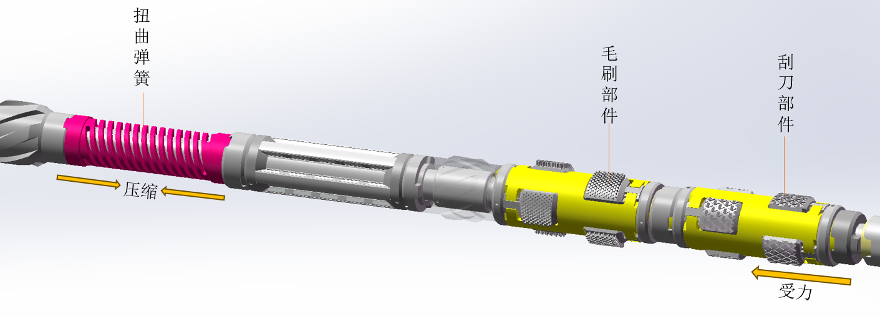
\includegraphics[width=.8\textwidth]{figure/chapter3/dynamic-system-torsional-spring-mechanism-4-in-1.png
}
	\caption{弹性刮削动力系统结构}
	\label{fig:flexible_scratch_system_4_in_1}
\end{figure}

\subsubsection{四合一工具辅助结构}

四合一工具辅助结构如图\ref{fig:additional_unite_4_in_1}所示。扶正器套装于心管外侧，轴向依靠上接头及下游组件的台阶端面限位，径向包覆螺纹连接部位。
扶正器外侧设计有螺旋导流槽，螺旋导流槽可以让钻井液/工作介质流过，不阻碍流体循环；支撑井壁使心管居中，承受径向摩擦载荷，保护心管与螺纹，改善工具下入性能。上接头作为四合一工具与外部管柱之间的连接部件，主要承担轴向载荷传递作用。其内部与心轴螺纹连接，使外部输入的轴向力能够有效传递至工具主体。
上接头外右侧空套一个扶正器。内六角凹端紧定螺钉使限制上接头与中心轴轴向移动，防止螺纹松动。

\begin{figure}[htbp]
    \centering
    % 子图 (a)
    \subfloat[上接头结构]{%
        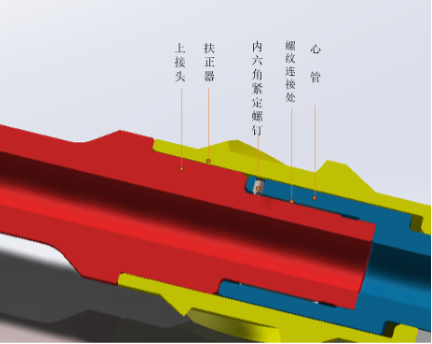
\includegraphics[width=0.4\linewidth]{figure/chapter3/upper-sub-4-in-1.png}%
        \label{fig:upper_sub_4_in_1}
    }
    %\hfill
    % 子图 (b)
    \subfloat[下接头结构]{%
        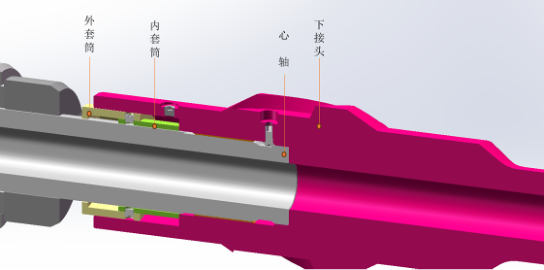
\includegraphics[width=0.5\linewidth]{figure/chapter3/lowwer-sub-4-in-1.png}%
        \label{fig:lowwer_sub_4_in_1}%
    }
    \caption{四合一工具辅助结构介绍}
        \label{fig:additional_unite_4_in_1}
\end{figure}

%\subsection{设计计算与校核}
\subsection[设计计算与校核]{设计计算与校核\protect\footnote{合同条款：5.2.1.3井筒高校清洁关键技术配套工具设计——（1）“四合一”集成式井筒清洁工具抗拉$>=100T$，抗扭$>17kN\cdot m$}}

%“2.75”-8 Stub ACME” 是一种常用于石油井下设备（如完井工具）的短牙梯形传动螺纹（Stub Acme Thread），ACME不是缩写，在机械工程领域，它特指 Acme Thread（爱克姆螺纹）。这是一种具有 29° 牙型角的梯形传动螺纹，其标准由美国标准协会（ANSI）制定。-8表示每英寸8个牙。
\subsubsection{主要受力件的螺纹强度校核}
四合一工具的主要受力件的螺纹强度危险点出现在心轴（图号：ZKG700004A）上，工具有三种规格，7\inch 规格的工具螺纹尺寸最小，最可能出现强度问题，于是螺纹抗拉强度校核以7\inch 规格作为计算依据，零件结构及尺寸如图\ref{fig:inner_pipe_for_strength_analysis}所示，其连接螺纹为2.75\inch -8 Stub ACME（爱克姆短牙梯形传动螺纹，8牙每英寸）。螺纹牙剪切强度计算：
\begin{equation}
\begin{aligned}
    F_{\max} &= [\tau] \cdot k_z \cdot \pi \cdot d_1 \cdot b \cdot z \cdot 10^{-3} \\
    [\tau] &= \frac{\sigma_s}{n}
\end{aligned}
\end{equation}
式中，$F_{\max}$---工具最大拉力，kN；

$[\tau]$---螺纹牙的剪切强度，MPa；

$k_z$---螺纹各圈的载荷不均系数，根据《机械设计手册》，取 $k_z = 0.56$；

$d_1$---螺纹底径，mm；

$b$---螺纹牙根宽度，mm；

$n$---安全系数，根据《机械设计手册》，取 $n = 2.5$；

$z$---旋合圈数；

$\sigma_s$---材料最小屈服强度，930 MPa (4330V-155 KSI)。
%4330V-155 KSI 是一种美标高强度低合金钢的牌号与强度等级组合标识，常用于石油、天然气及航空航天等对材料强度和韧性要求极高的领域。4330V：这是美国钢铁协会（AISI）标准下的合金结构钢牌号，属于镍铬钼钒系钢。它在4330钢的基础上添加了钒（V），以提升强度、硬度和抗疲劳性能。该材料通常经过真空电弧重熔（VAR）工艺处理，具有优异的淬透性、低温冲击韧性和抗裂纹扩展能力。155 KSI：表示该材料经热处理后达到的最小屈服强度为155千磅每平方英寸（KSI），换算约为1069 MPa。这属于超高强度级别，适用于承受极端载荷和冲击的工况。这种钢材的典型应用包括石油钻具、井下工具、航空紧固件和高应力传动部件。其化学成分中碳含量约0.28–0.33%，镍含量2.0–2.5%，铬0.6–0.9%，钼0.2–0.3%，钒0.15–0.3%，这些元素共同赋予其高强度与高韧性的平衡。

$2.75\inch - 8 \text{Stub ACME}$ 螺纹代入数据计算如下：
\begin{align*}
    F_{\max} &= [\tau] \cdot k_z \cdot \pi \cdot d_1 \cdot b \cdot z \cdot 10^{-3} \\
    &= 372 \times 0.56 \times 3.14 \times 67.94 \times 1.833 \times 35 \times 10^{-3} = 2851.13 \text{kN} \\
    &> 1000 \text{kN}
\end{align*}
于是，螺纹满足抗拉设计要求。

\begin{figure}[htbp]
	\centering
	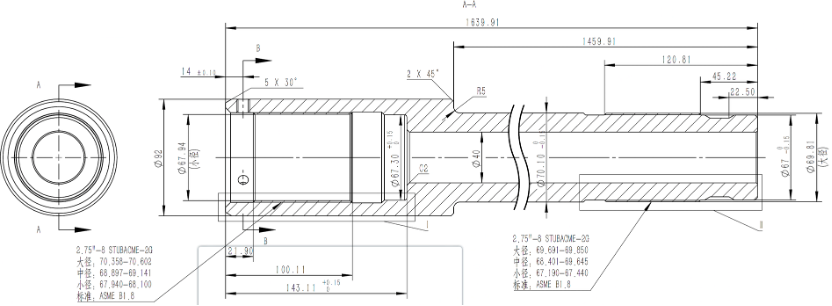
\includegraphics[width=1.\textwidth]{figure/chapter3/inner-pipe-for-strength-analysis.png}
	\caption{7\inch 规格工具的心轴结构}
	\label{fig:inner_pipe_for_strength_analysis}
\end{figure}

\subsubsection{主要受力件的零件强度校核}

清洁工具的主要受力件为芯轴危险截面有两处，分别为2.75”-8 Stub ACME外螺纹根部、2.75”-8 Stub ACME内螺纹根部。本文用解析法、数值模拟两种方法对心轴的强度进行校核。

（1）芯轴抗拉危险截面1：为2.75”-8 Stub ACME外螺纹根部。

对于环形零件截面，抗拉强度计算公式：
\begin{equation}
    F_{\max} = \frac{[\pi \cdot (D^2 - d^2)] \cdot \sigma_s}{4 \cdot n} \times 10^{-3}
    \label{eq:tensile_strength_circular_section}
\end{equation}
式中，$F_{\max}$——工具最大拉力，kN；

$D$——危险截面外径，mm；

$d$——危险截面内径，mm；

$\sigma_s$——材料最小屈服强度：930 MPa (4330V-155 KSI)；

$n$——安全系数，取 $n = 1.5$。

根据图\ref{fig:inner_pipe_for_strength_analysis}，取$D=67\textrm{mm}$，$d=40\textrm{mm}$，则心轴上$2.75\inch - 8 \cdot \text{Stub ACME}$ 外螺纹根部最大拉力：
\begin{align}
    F_{\max} &= \frac{\pi \cdot (D^2 - d^2) \cdot \sigma_s}{4 \cdot n} \times 10^{-3} \nonumber \\
    &= \frac{3.14 \times (67^2 - 40^2) \times 930}{4 \times 1.5} \times 10^{-3} \nonumber \\
    &= 1408.06 \, \text{kN} > 1000 \, \text{kN}
\end{align}

于是，危险截面1满足抗拉设计要求。

（2）心轴抗拉危险截面 2：为 $2.75\inch - 8 \text{Stub ACME}$ 内螺纹根部。

根据公式\ref{eq:tensile_strength_circular_section}和图\ref{fig:inner_pipe_for_strength_analysis}，取$D=92\textrm{mm}$。$d=71.6\textrm{mm}$（参见图纸ZKG700004A局部视图I），则心轴上$2.75\inch - 8 \text{Stub ACME}$ 外螺纹根部最大拉力：
\begin{align}
    F_{\max} &= \frac{[\pi \cdot (D^2 - d^2) ] \cdot \sigma_s}{4 \cdot n} \times 10^{-3} \nonumber \\
    &= \frac{[3.14 \times (92^2 - 71.6^2) ] \times 930}{4 \times 1.5} \times 10^{-3} \nonumber \\
    &= 1624.30 \, \text{kN} > 1000 \, \text{kN}
\end{align}

于是，危险截面2满足拉伸强度设计要求。


\subsubsection{主要受力件的零件强度抗扭校核}

四合一工具的受扭危险零件依然为\ref{fig:inner_pipe_for_strength_analysis}心轴螺纹结构根部截面，以及用于零件之间周向定位的端面键，如图\ref{fig:flat_shear_key}所示。下面进行螺纹危险截面的抗扭强度计算。截面抗扭强度$T_{\max}$计算式为
\begin{figure}[htbp]
	\centering
	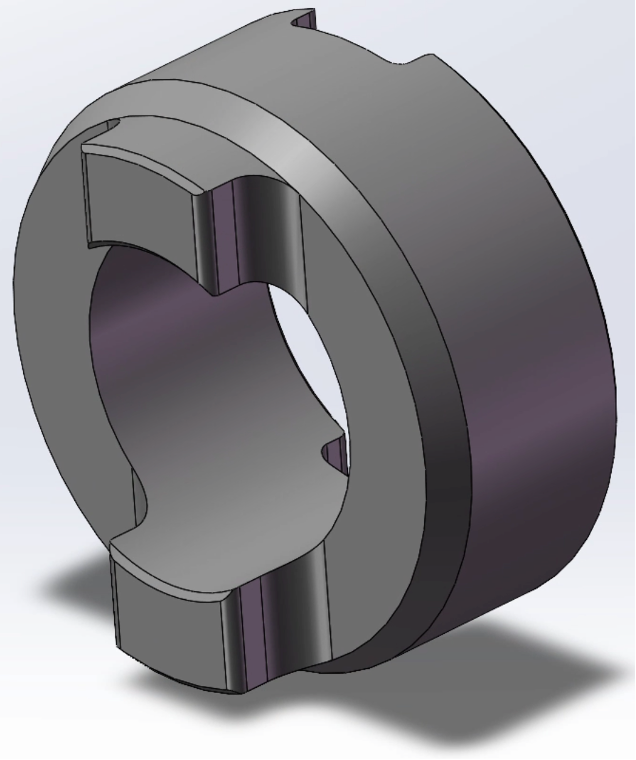
\includegraphics[width=.4\textwidth]{figure/chapter3/flat-shear-key.png}
	\caption{端面抗扭键结构}
	\label{fig:flat_shear_key}
\end{figure}

%\tau & =  \frac{16 \cdot D \cdot T_{\max}}{\pi \cdot (D^4 - d^4)} \times 10^6\\
\begin{equation}
\begin{aligned}	
    T_{\max} & =  \frac{[\tau] \cdot \pi \cdot (D^4 - d^4)}{16 \cdot D} \times 10^{-6}\\
    [\tau] &= n \cdot \sigma_s 
    \end{aligned}
\end{equation}
式中，$T_{\max}$——工具最大扭矩，kN·m；

$D$——危险截面外径，mm；

$d$——危险截面内径，mm；

$\sigma_s$——材料屈服应力，MPa；

$n$——安全系数，根据《机械设计手册》，取$n = 0.66$；

$[\tau]$——材料许用切应力，MPa。

对于心轴的危险截面1，代入材料的力学和几何参数计算得
\begin{align}
    T_{\max} &= \frac{[\tau] \cdot \pi \cdot (D^4 - d^4)}{16 \cdot D} \times 10^{-6} \nonumber \\
    &= \frac{613.8 \times 3.14 \times (67^4 - 40^4)}{16 \times 67} \times 10^{-6} \nonumber \\
    &= 31.63\,\text{kN} \cdot \text{m} > 17\,\text{kN} \cdot \text{m}
\end{align}

对于危险截面2，代入材料的力学和几何参数计算得
\begin{align}
    T_{\max} &= \frac{[\tau] \cdot \pi \cdot (D^4 - d^4)}{16 \cdot D} \times 10^{-6} \nonumber \\
    &= \frac{613.8 \times 3.14 \times (92^4 - 71.6^4)}{16 \times 92} \times 10^{-6} \nonumber \\
    &= 59.39\,\text{kN} \cdot \text{m} > 17\,\text{kN} \cdot \text{m}
\end{align}

于是，工具的两个危险截面都满足抗扭强度要求。

有限元计算结果如图所示。主要受力件为芯轴，危险截面出现在变径处，最大拉应力为1379MPa，最大剪切力为937MPa，建议在危险截面增加圆角以减小应力集中。

\begin{figure}[htbp]
	\centering
	\subfloat[拉伸载荷下应力分布]{%
	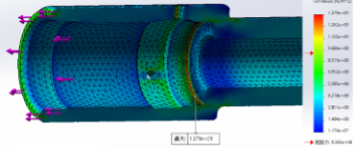
\includegraphics[width=0.7\textwidth]{figure/chapter3/inner-pipe-tensile-strength-simulation.png}
	}
	\vspace{1em}
	\subfloat[扭转载荷下应力分布]{%
	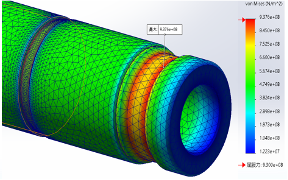
\includegraphics[width=0.7\textwidth]{figure/chapter3/inner-pipe-torsional-strength-simulation.png}
	}
	\caption{心轴零件受力有限元分析}
	\label{fig:FEA_verification_shaft}
\end{figure}

对于端面键，其材料牌号为4145H，抗扭危险截面为端面键截面（键的数量为 2）。

外筒件抗扭强度 $\tau$ 计算：
\begin{align}
    \tau &= \frac{T_{\max}}{b \cdot h \cdot d} \times 10^{-6} \\
    T_{\max} &= \frac{[\tau] \cdot b \cdot h \cdot d}{n_1} \times 10^{-6} \\
    [\tau] &= n \cdot \sigma_s = 0.66 \times 827\,\text{MPa} = 545.82\,\text{MPa}
\end{align}
式中，$T_{\max}$ —— 扭矩，$\text{kN}\cdot\text{m}$；

    $\sigma_s$ ——材料屈服应力，$\text{Mpa}$；
    
    $d$ ——危险截面内径，$\text{mm}$；
    
    $b$ ——端面键宽度，$\text{mm}$；
    
    $h$ ——端面键高度，$\text{mm}$；
    
    $n$ ——许用剪应力与许用拉应力系数，根据《机械设计手册》，取 $n=0.66$；
    
    $[\tau]$ ——材料许用切应力，$\text{Mpa}$；
    
    $n_1$ ——安全系数，取 $n_1=1.5$。

外筒件能承受的最大扭矩：
\begin{equation}
    T_{\max} = \frac{[\tau] \cdot b \cdot h \cdot d}{n_1} \times 10^{-6} = \frac{545.82 \times 30 \times 13.5 \times 90}{1.5} \times 10^{-6} = 13.29\,\text{kN}\cdot\text{m}
\end{equation}


\subsubsection{弹簧的力学计算}

四合一工具中设计了毛刷和刮板的预紧弹簧以及蓄能弹簧，如图\ref{fig:spring}所示。
\begin{figure}[htbp]
	\centering
	\subfloat[刮板、毛刷预紧弹簧]{%
	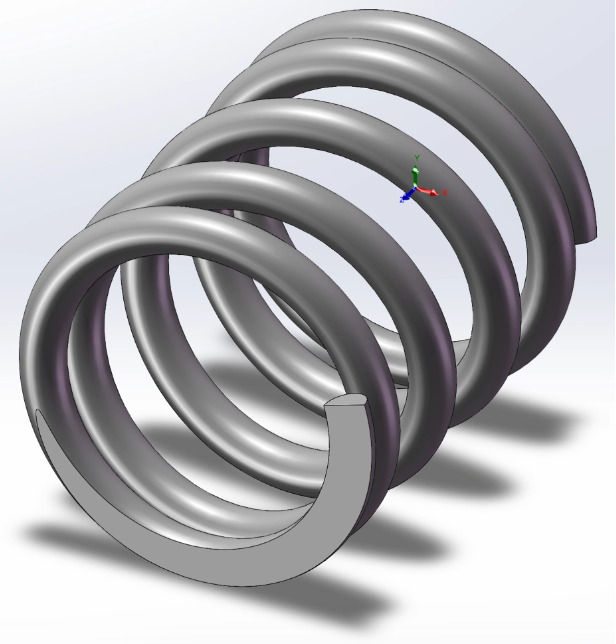
\includegraphics[width=0.2\textwidth]{figure/chapter3/pitch-spring.png}
	}
	%\vspace{1em}
	\subfloat[蓄能弹簧]{%
	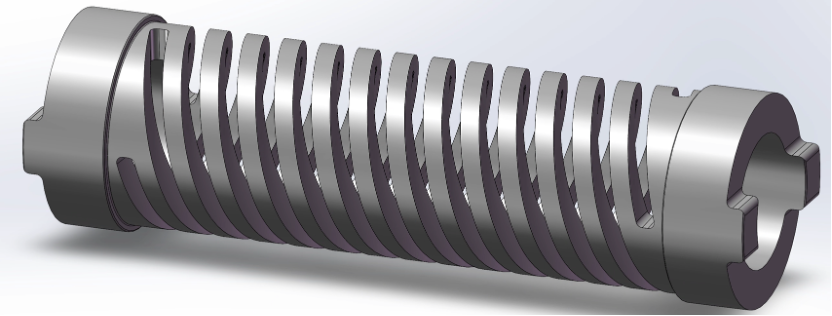
\includegraphics[width=0.55\textwidth]{figure/chapter3/oscillating-spring.png}
	}
	\caption{四合一工具中的弹簧零件}
	\label{fig:spring}
\end{figure}

毛刷和刮板的预紧弹簧参数列举于表\ref{tab:spring_parameters_pitch}，蓄能弹簧的参数列举于表\ref{tab:spring_params_rebounce}。
\begin{table}[htbp]
    \centering
    \caption{毛刷与刮板预紧弹簧技术参数表}
    \label{tab:spring_parameters_pitch}
    \renewcommand{\arraystretch}{1.3} % 增加行高，使表格更美观
    \begin{tabularx}{0.8\textwidth}{Xc}
        \toprule % 顶线
        \textbf{参数名称} & \textbf{数值} \\
        \midrule % 栏目线
        弹簧外径 $D$ & 25\,mm \\
        弹簧内径 $D_1$ & 19\,mm \\
        弹簧中径 $D_2$ & 22\,mm \\
        弹簧线径 $d$ & 3\,mm \\
        弹簧剪切弹性模量 $G$ & 79\,GPa \\
        弹簧自由高度 $H$ & 35\,mm \\
        弹簧总圈数 $n_1$ & 5 \\
        弹簧有效圈数 $n$ & 3 \\
        最小工作高度 $H_1$ & 29\,mm \\
        最大工作高度 $H_2$ & 23\,mm \\
        许用切应力 $[\tau]$ & 710\,MPa \\
        \bottomrule % 底线
    \end{tabularx}
\end{table}

\begin{table}[htbp]
    \centering
    \caption{弹簧技术参数表}
    \label{tab:spring_params_rebounce}
    \renewcommand{\arraystretch}{1.5} % 增加行高，使表格更美观
    \begin{tabularx}{0.8\textwidth}{Xc}  
        \toprule % 顶线
        \textbf{参数名称} & \textbf{数值} \\
        \midrule % 栏目线
        弹簧外径 $D$ & 120\,mm \\
        弹簧内径 $D_1$ & 80\,mm \\
        弹簧中径 $D_2$ & 100\,mm \\
        弹簧截面宽度 $b$ & 20\,mm \\
        弹簧截面高度 $h$ & 20\,mm \\
        弹簧剪切弹性模量 $G$ & 79\,GPa \\
        弹簧系数 $\gamma'$ & 5.57 \\
        弹簧系数 $\beta'$ & 2.404 \\
        弹簧自由高度 $H$ & 440\,mm \\
        弹簧总圈数 $n_1$ & 11 \\
        弹簧有效圈数 $n$ & 9 \\
        最小工作高度 $H_1$ & 400\,mm \\
        最大工作高度 $H_2$ & 390\,mm \\
        许用切应力 $[\tau]$ & 710\,MPa \\
        \bottomrule % 底线
    \end{tabularx}
\end{table}

刮刀与毛刷弹簧的力学计算如下。


弹簧刚度$P'$为
\begin{equation}
    P' = \frac{G \cdot d^4}{8 \cdot D_2^3 \cdot n} \times 10^{-3} = \frac{79000 \times 3^4}{8 \times 22^3 \times 3} \times 10^{-3} = 25 \, \text{N/mm}
\end{equation}

弹簧最小工作载荷$P_1$
\begin{equation}
    P_1 = P' \cdot (H - H_1) = 22 \times (35 - 29) = 132 \, \text{N}
\end{equation}

弹簧最大工作载荷$P_n$
\begin{equation}
    P_n = P' \cdot (H - H_2) = 22 \times (35 - 23) = 264 \, \text{N}
\end{equation}

弹簧旋绕比$C$
\begin{equation}
    C = \frac{D_2}{d} = \frac{22}{3} = 7.33
\end{equation}

弹簧曲度系数$K$
\begin{equation}
    K = \frac{4 \cdot C - 1}{4 \cdot C - 4} + \frac{0.615}{C} = \frac{4 \times 7.33 - 1}{4 \times 7.33 - 4} + \frac{0.615}{7.33} = 1.2
\end{equation}

弹簧最大切应力$\tau_{\max}$
\begin{equation}
    \tau_{\max} = \frac{8 \cdot K \cdot D_2}{\pi \cdot d^3} \times P_n = \frac{8 \times 1.2 \times 22}{3.14 \times 3^3} \times 264 = 657.7 \, \text{MPa} < 710 \, \text{MPa}
\end{equation}

于是，刮刀与毛刷强度满足要求。

蓄能弹簧的力学计算如下。

弹簧模块刚度$P'$
\begin{equation}
    P' = \frac{G \cdot b^2 \cdot h^2}{\gamma' \cdot D_2^3 \cdot n} = \frac{79000 \times 20^2 \times 20^2}{5.57 \times 100^3 \times 9} = 252 \, \text{N/mm}
\end{equation}

弹簧最小工作载荷$P_1$
\begin{equation}
    P_1 = P' \cdot (H - H_1) = 252 \times (440 - 400) = 10080 \, \text{N}
\end{equation}

弹簧最大工作载荷$P_n$
\begin{equation}
    P_n = P' \cdot (H - H_2) = 252 \times (440 - 390) = 12600 \, \text{N}
\end{equation}

弹簧旋绕比$C$
\begin{equation}
    C = \frac{D_2}{h} = \frac{100}{20} = 5
\end{equation}

弹簧曲度系数$K$
\begin{equation}
    K = \frac{4 \cdot C - 1}{4 \cdot C - 4} + \frac{0.615}{C} = \frac{4 \times 5 - 1}{4 \times 5 - 4} + \frac{0.615}{5} = 1.31
\end{equation}

弹簧最大切应力$\tau_{\max}$
\begin{equation}
    \tau_{\max} = \frac{\psi \cdot K \cdot D_2}{b \cdot h \cdot \sqrt{b \cdot h}} \cdot P_n = \frac{2.404 \times 1.31 \times 100}{20 \times 20 \times \sqrt{20 \times 20}} \times 12600 = 496 \, \text{MPa} < 710 \, \text{MPa}
\end{equation}

于是，蓄能弹簧的强度满足设计要求。



综合上述，各主要受力件的性能数据统计于表\ref{tab:force_data_statistics}中。


\begin{table}[htbp]
    \centering
    \caption{受力件数据统计表}
    \label{tab:force_data_statistics}
    \renewcommand{\arraystretch}{1.4} % 增加行高
    \begin{tabularx}{0.8\textwidth}{Xc}  % 关键：使用 tabularx + \textwidth + X列
        \toprule
        受力类型 & 数据\\
        \midrule
        NC38 最大拉力 & $3000\,\text{kN}$ \\
        材料屈服强度 $\sigma_s$ & $930\,\text{MPa}$ \\
        螺纹最大剪切力 $F_{\max1}$ & $2851.13\,\text{kN}$ \\
        芯轴最大拉力 $F_{\max2}$ & $1408.06\,\text{kN}$ \\
        NC38 最大扭矩 & $44.3\,\text{kN}\cdot\text{m}$ \\
        材料许用切应力 $[\tau]$ & $613.8\,\text{MPa}$ \\
        芯轴最大扭力 $T_{\max1}$ & $31.63\,\text{kN}\cdot\text{m}$ \\
        弹簧许用切应力 & $710\,\text{MPa}$ \\
        弹簧刚度 $P'$ & $22\,\text{N/mm}$ \\
        弹簧最小工作载荷 $P_1$ & $132\,\text{N}$ \\
        弹簧最大工作载荷 $P_n$ & $264\,\text{N}$ \\
        弹簧旋绕比 $C$ & $7.33$ \\
        弹簧曲度系数 $K$ & $1.2$ \\
        弹簧最大切应力 $\tau_{\max}$ & $657.7\,\text{MPa}$ \\
        外筒件抗扭 $T_{\max2}$ & $13.29\,\text{kN}\cdot\text{m}$ \\
        \bottomrule
    \end{tabularx}
\end{table}
	% !TeX root = ../../main.tex
\subsection{刮板刮削效果评价}
\label{guaban}
在工程应用中刮板相对于套管是直线运动，在实验室中复现该过程对设备要求高。考虑到工具上的主要功能结构——刮板通过与套管（垢）之间的相对运动产生清洁作用，在装置设计时抓住“相对运动”这一主要矛盾即可对刮板的使役性能进行模拟。

本项目设计了基于转盘的刮板刮削能力评价装置，其结构和工作原理如图\ref{fig:scraper_test_rig_mechanism}所示。该装置中，刮板与机架固连，铺设于转盘表面的垢主动旋转以产生相对运动（刮板的主切削运动）。刮板与垢之间是线（面）接触，二者并非严格意义上的相对平动，需对两者的差异作量级估算。转盘表面可视作套管内壁沿周向展开的平面：转盘切向（旋转方向）对应套管轴向即刮板行程方向，径向对应套管内壁的周向位置。本装置转盘半径为0.5 m，刮刀两端距盘心分别为$r_1 = 27\,\text{cm}$与$r_2 = 40\,\text{cm}$，接触区平均半径$\bar r=33.5$ cm。垢随转盘定轴转动时，接触区内各点的相对运动方向均沿切向且与刮刀刃线垂直，与直线平动在方向上一致。垢面上任一材料点的刮削仅发生在它经过刮刀正下方的瞬时接触过程中，对应的滑动距离等于刮刀刀齿沿运动方向的接触宽度$w$（毫米至厘米量级），远小于$\bar r$；在该接触过程中，材料点的运动路径为弧长$w$的圆弧，其相对直线的最大垂向偏差约为$w^2/(8\bar r)$（不超过0.1 mm），故局部刮削过程与直线平动等价。单次拉动刮痕的总长度由扇形垢样包角（约90°）决定，在垢样带内约为0.5 m，仅决定刮痕长度，不改变局部去除机理。接触区内沿刮刀径向跨度各点线速度$v=\omega r$不同，内、外端线速度之比$r_2/r_1\approx1.48$，相对平均速度的最大偏差约为$\pm19\%$，即当平均线速度约为0.05 m/s时，内、外端线速度分别约为0.040 m/s与0.060 m/s。该速度范围处于低速准静态区，硬垢的脆性崩碎去除机理对线速度不敏感。因此，以旋转盘面代替直线平动，对本节刮削效果的相对评价是可行的。

\begin{figure}[htbp]
	\centering
	\subfloat[实验装置结构及原理]{%
	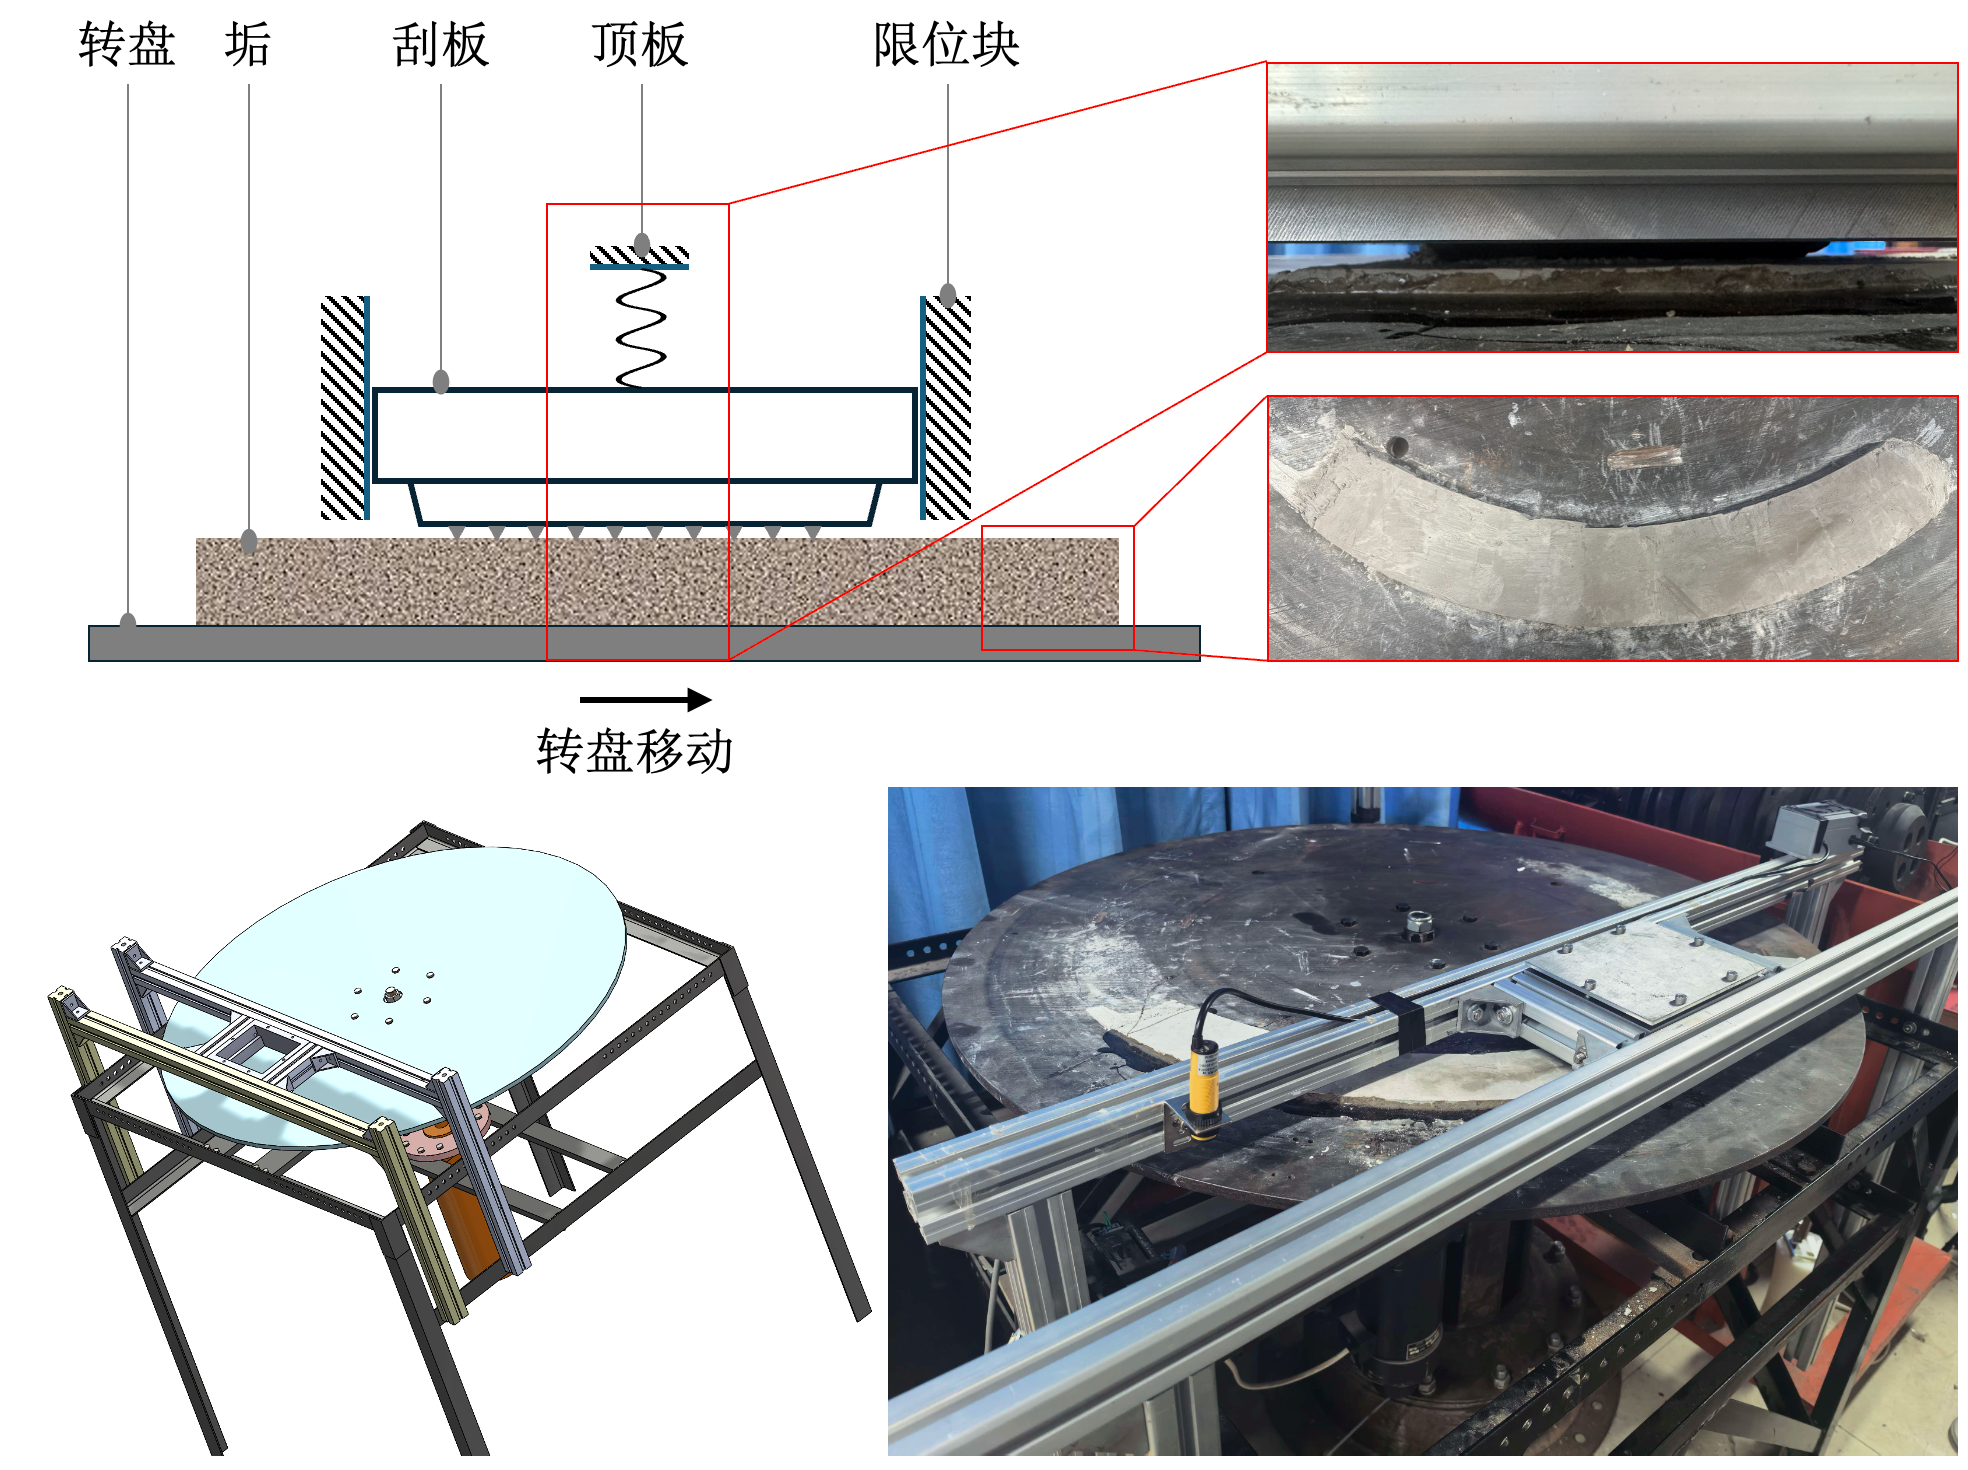
\includegraphics[width=.9\textwidth]{figure/chapter3/scraper-test-rig.png}
	\label{fig:scraper_test_rig_mechanism}
	}
	\vspace{1em}
	\subfloat[弹簧变形量测量原理]{%
	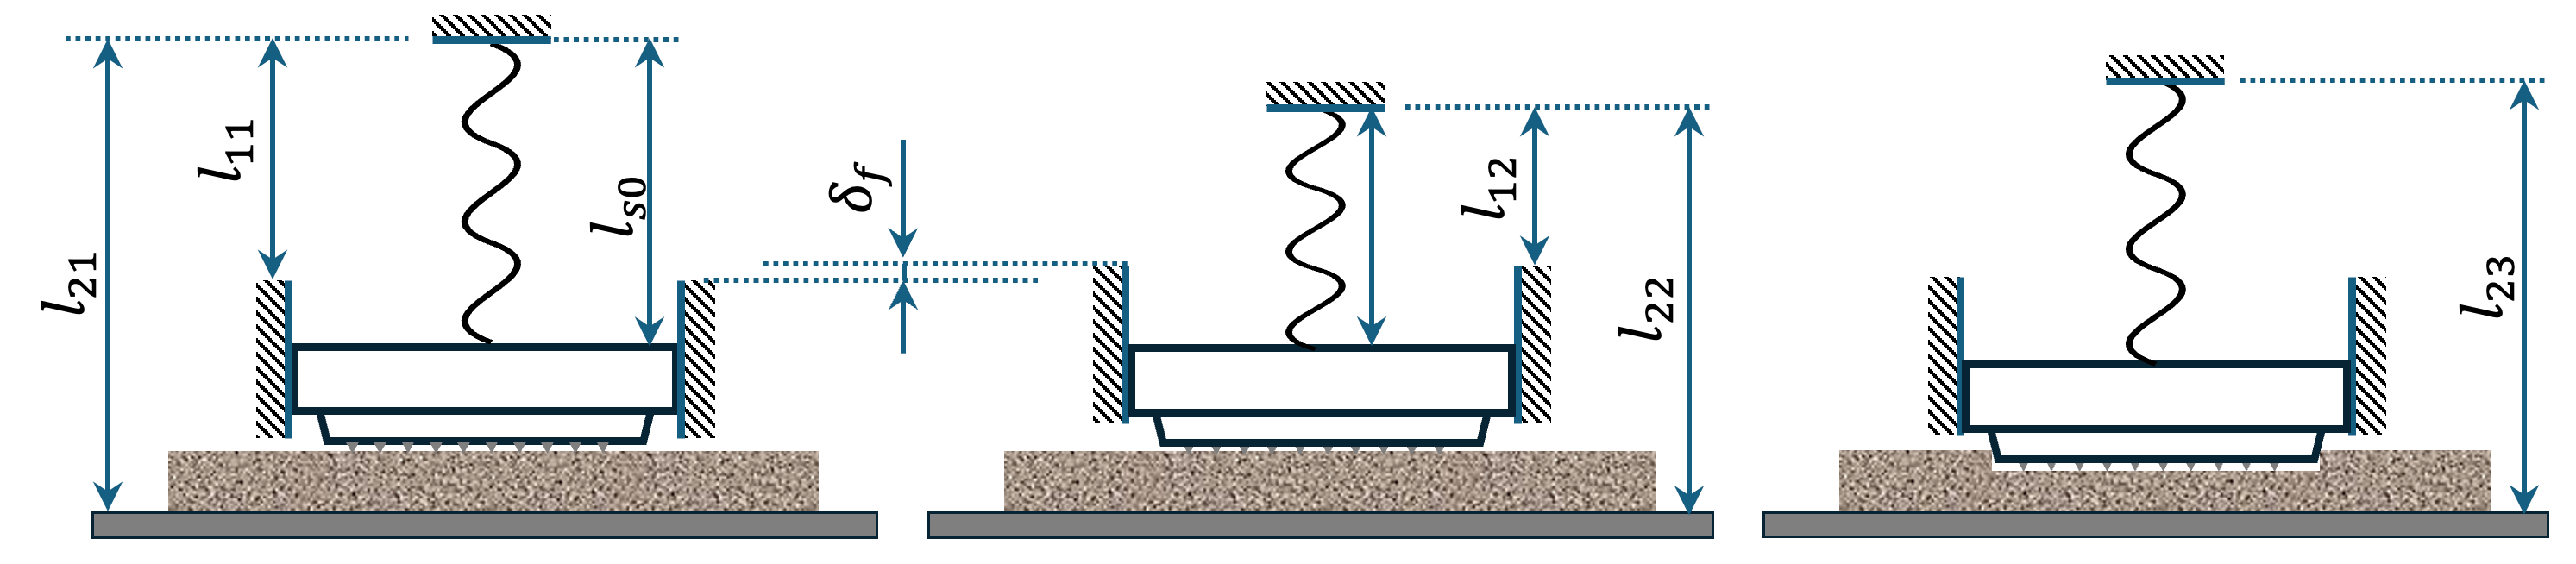
\includegraphics[width=.9\textwidth]{figure/chapter3/scapter-measurement-mechanism.png}
	\label{fig:scapter_measurement_mechanism}
	}
	\caption{刮板刮削性能测试}
	\label{fig:scraper_test_rig}
\end{figure}

试验用垢样为模拟硬垢，其矿物成分以重晶石（硫酸钡）为主，用于近似模拟现场以硫酸钡/钡锶垢为主的坚硬垢层。制作时，将重晶石粉与硫铝酸盐水泥按质量比3:4干混均匀，加水拌合至浆体呈黏糊状态，浇注于放置在转盘盘面上的扇形模具中成形，养护至规定龄期后得到与转盘盘面粘接的扇形垢样。垢样位于距转盘中心半径30\textasciitilde{}38 cm的环形带内（内半径30 cm、外半径38 cm、厚度10 cm），垢样带外缘直径为0.76 m，本装置转盘半径为0.5 m（直径1 m），可满足垢样布置要求；扇形垢样沿周向的包角约为90°。为防止刮削过程中垢样边缘起翘、开裂或整体滑移，每块扇形垢样的两侧边缘均以环氧树脂与转盘盘面粘接固定。环氧树脂固定带及垢样台阶边缘处的刮削状态不具有代表性，故各测量点均布置在扇形垢样中部、距两侧环氧固定带一定距离的区域内，以保证刮削前后测量位置一致。垢样厚度（10 cm）远大于刮削深度（毫米级），刮削过程中垢层可视为半无限厚基体，转盘金属基底对刮削结果的影响可以忽略。为表征垢样的力学属性，同期以相同配比、相同工艺浇注了试块，用于测定垢样的抗压强度与硬度。

刮板是靠弹簧支撑的，为了模拟刮板的这种“浮动”支撑效果，在装置上设置了限位块约束刮板五个运动自由度，保留一个沿盘面法线方向的移动自由度。实验中，限位块用大跨距的横梁与机架固连，在刮板与垢之间的背向力较大时，可能产生挠曲变形$\delta _f$，需在计算弹簧压缩量$\delta_s$时进行补偿。

% 作者待补/核对：①扇形垢样块数及单次刮削流程（包角约90°、转盘半径0.5 m已确认）；②养护条件与龄期；③垢样抗压强度、硬度实测值及正文引用处；④刮刀刀齿沿运动方向接触宽度w的量级（正文按“毫米至厘米、垂向偏差不超过0.1 mm”定性表述，若实测请补具体值）；⑤手拉线速度0.05 m/s的测量位置（正文按接触区平均半径33.5 cm处表述）；⑥各尺寸测量基准面是否统一取垢样顶面。
实验记录的数据含义如图\ref{fig:scapter_measurement_mechanism}所示。实验前，先让弹簧处于原长状态，测量距离$l_{11}$和$l_{21}$，这两个尺寸分别是顶板顶部测量基面和限位块顶部、转盘盘面之间的距离。然后，根据弹簧的参考压缩量，将弹簧预紧，测量$l_{11}$、$l_{21}$，记为$l_{12}$、$l_{22}$。转动转盘，使刮板完成一次刮削过程，停止设备后，再次测量尺寸$l_{21}$，记为$l_{23}$。从实验台上取一个参考位置，在划痕的两侧取两个监测点，测量监测点相对于参考位置之间的距离$l_{31}$、$l_{32}$，再测量刮削坑的底部与参考点之间的距离$l_4$。实验中的尺寸测量采用的是精度为0.02 mm的游标卡尺，且刮削前后的尺寸测量均在同一扇形垢样区、同一测量位置完成，以保证测量基准一致。



根据几何关系，单次刮削产生的坑深度$\delta_c$、坑的累积深度$\delta_c'$，弹簧压缩量估计值$\delta_s$为
\begin{equation}
\centering
	\begin{aligned}
		\delta_c' & =l_4-\frac{l_{31}+l_{32}}{2}\\
		\delta_f & = l_{23}-l_{21}  \\ 
		\delta_s & = l_{11}-l_{12} - \delta_f- \delta_c'
	\end{aligned}
\end{equation}

垢经刮削后的形貌如图\ref{fig:scale_profile}所示。刮板前刀面附近堆积有粉末状和崩碎状屑，刀齿的容屑槽中也有此类屑，由此证明，所设计的刮板能有效刮除硬垢。在刮削区域的边缘也有这样的屑。从切屑的性质可以推测出，所设计的垢为脆性垢，与文献所述的垢性质吻合。%补充是哪一篇文献
从图中还可以看出，产屑量与弹簧的压缩量成正相关。
\begin{figure}[htbp]
	\centering
	\subfloat[$\delta_s=3.095\textrm{mm}$]{%
	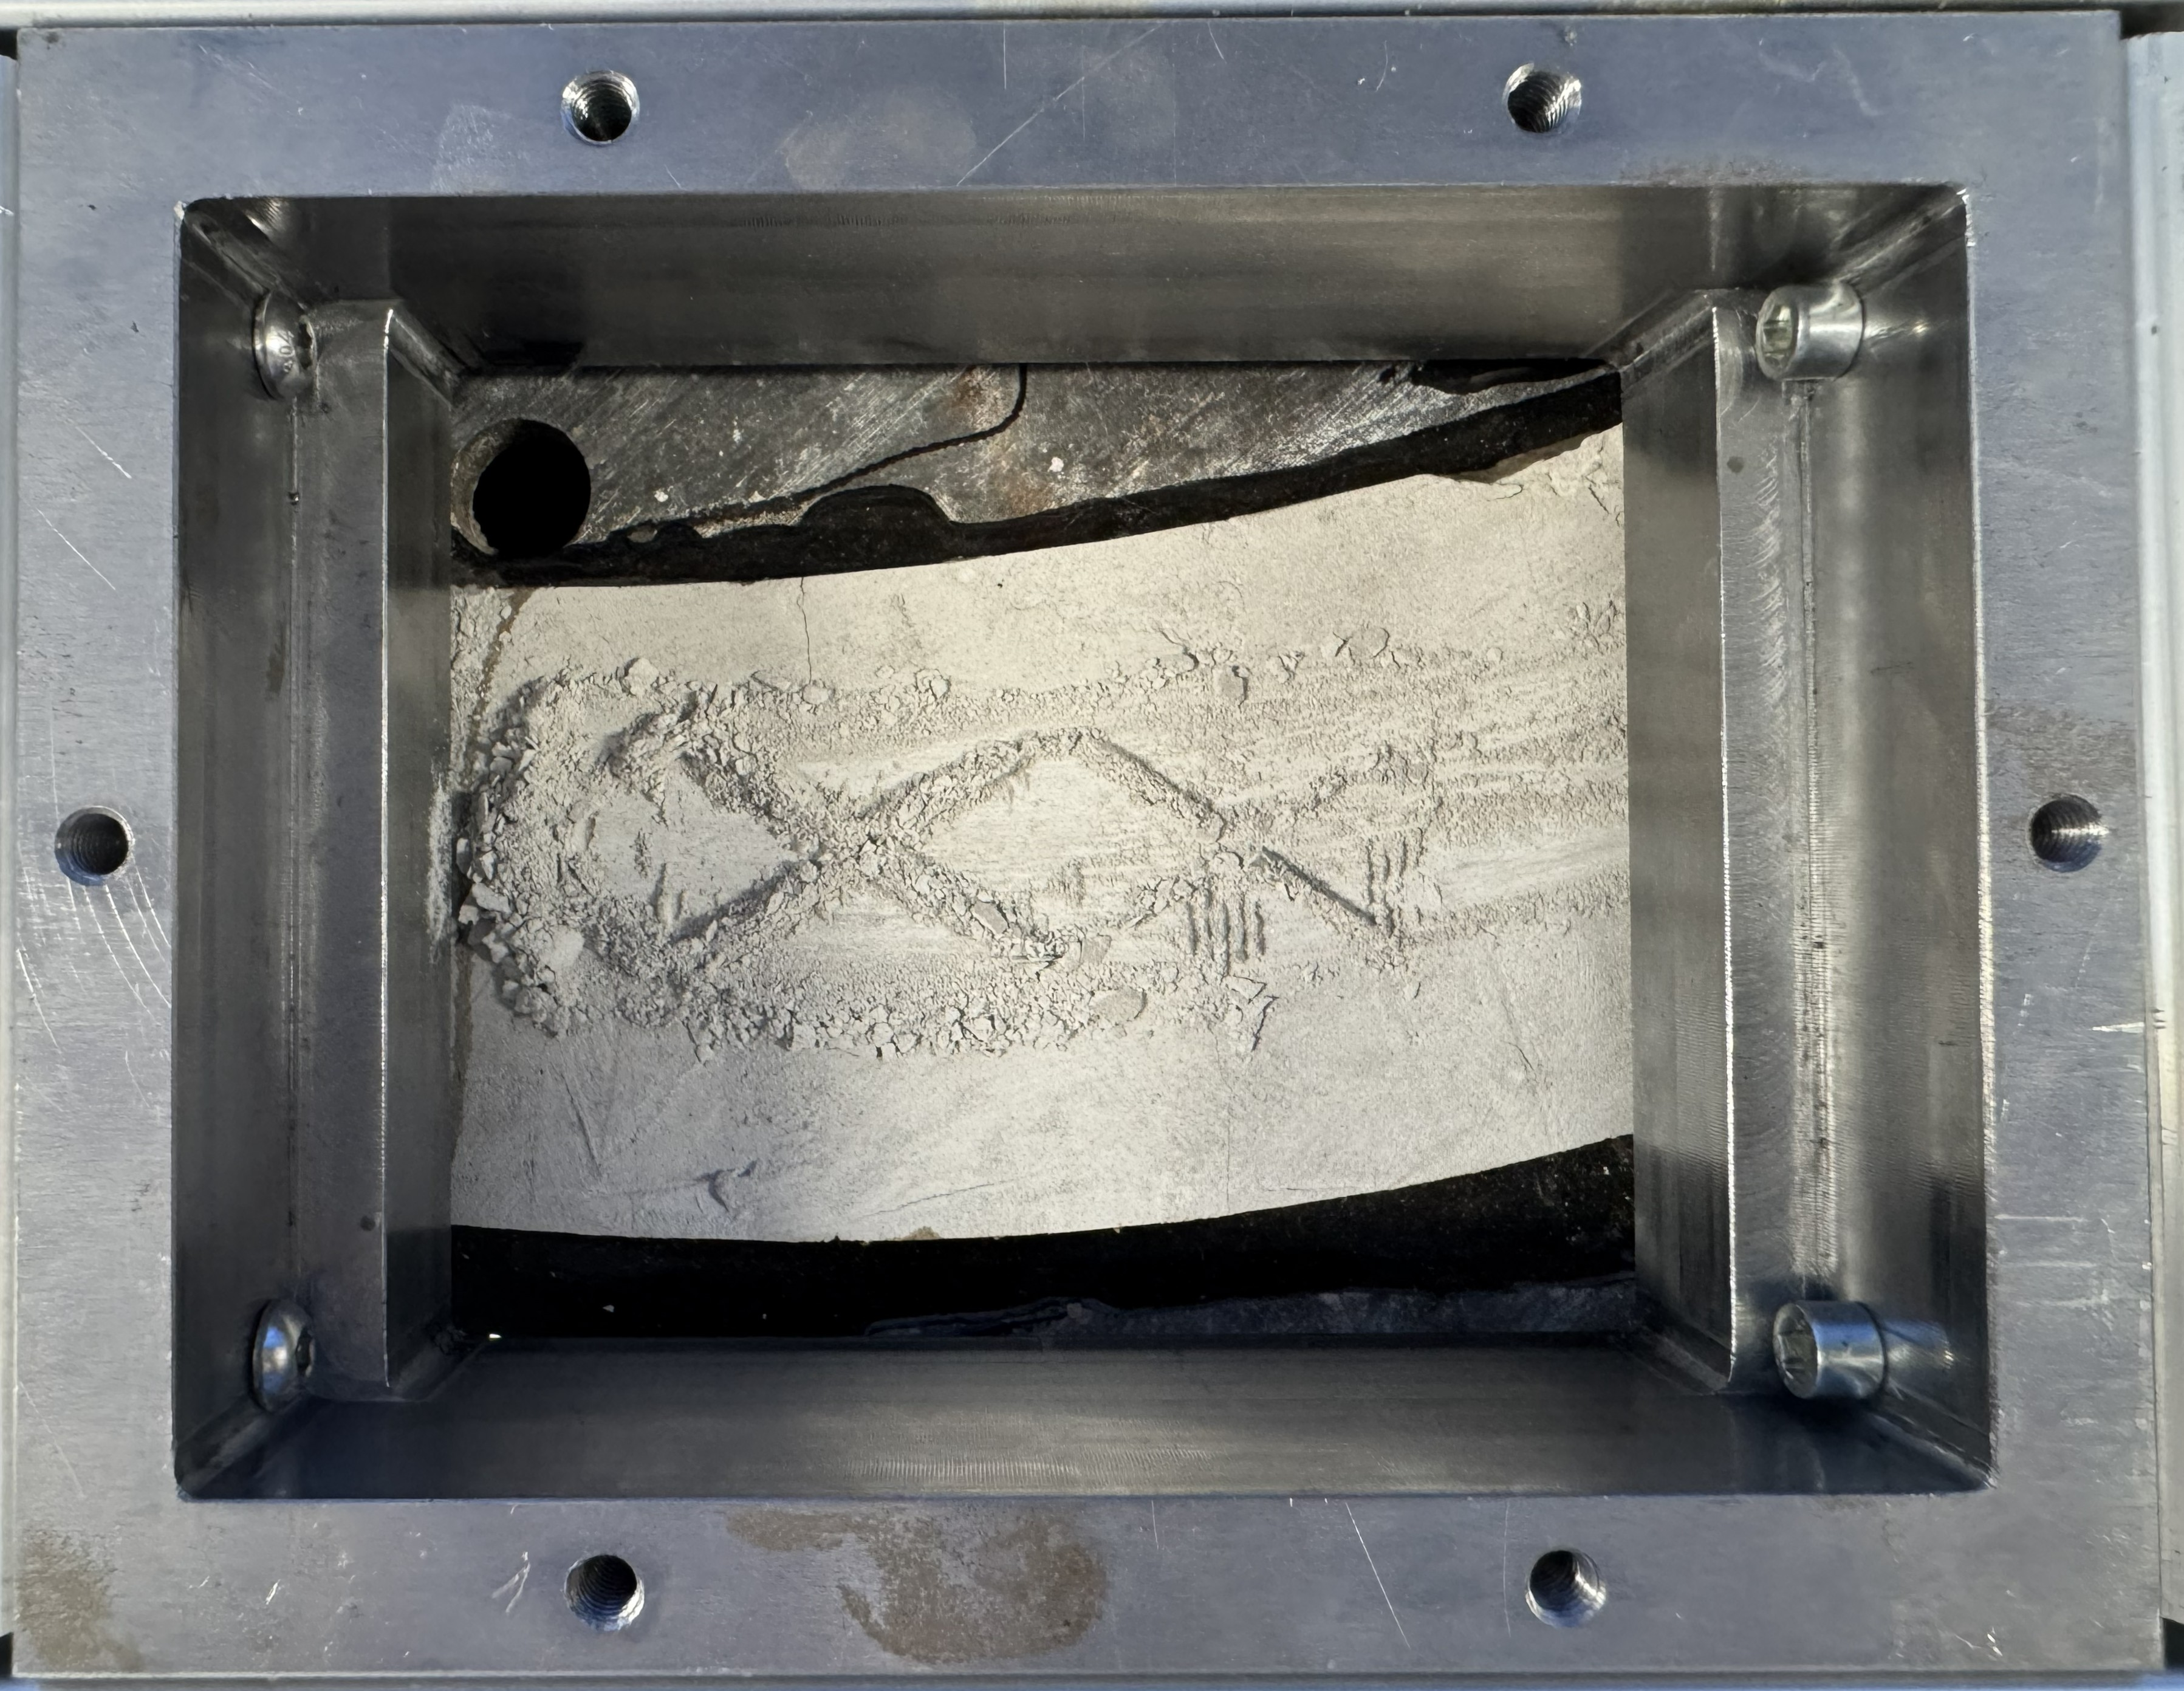
\includegraphics[height=4.0cm]{figure/chapter3/scale-1.jpg}
	\label{fig:scale_1}
	}
	%\hfill
	\subfloat[$\delta_s=4.875\textrm{mm}$]{%
	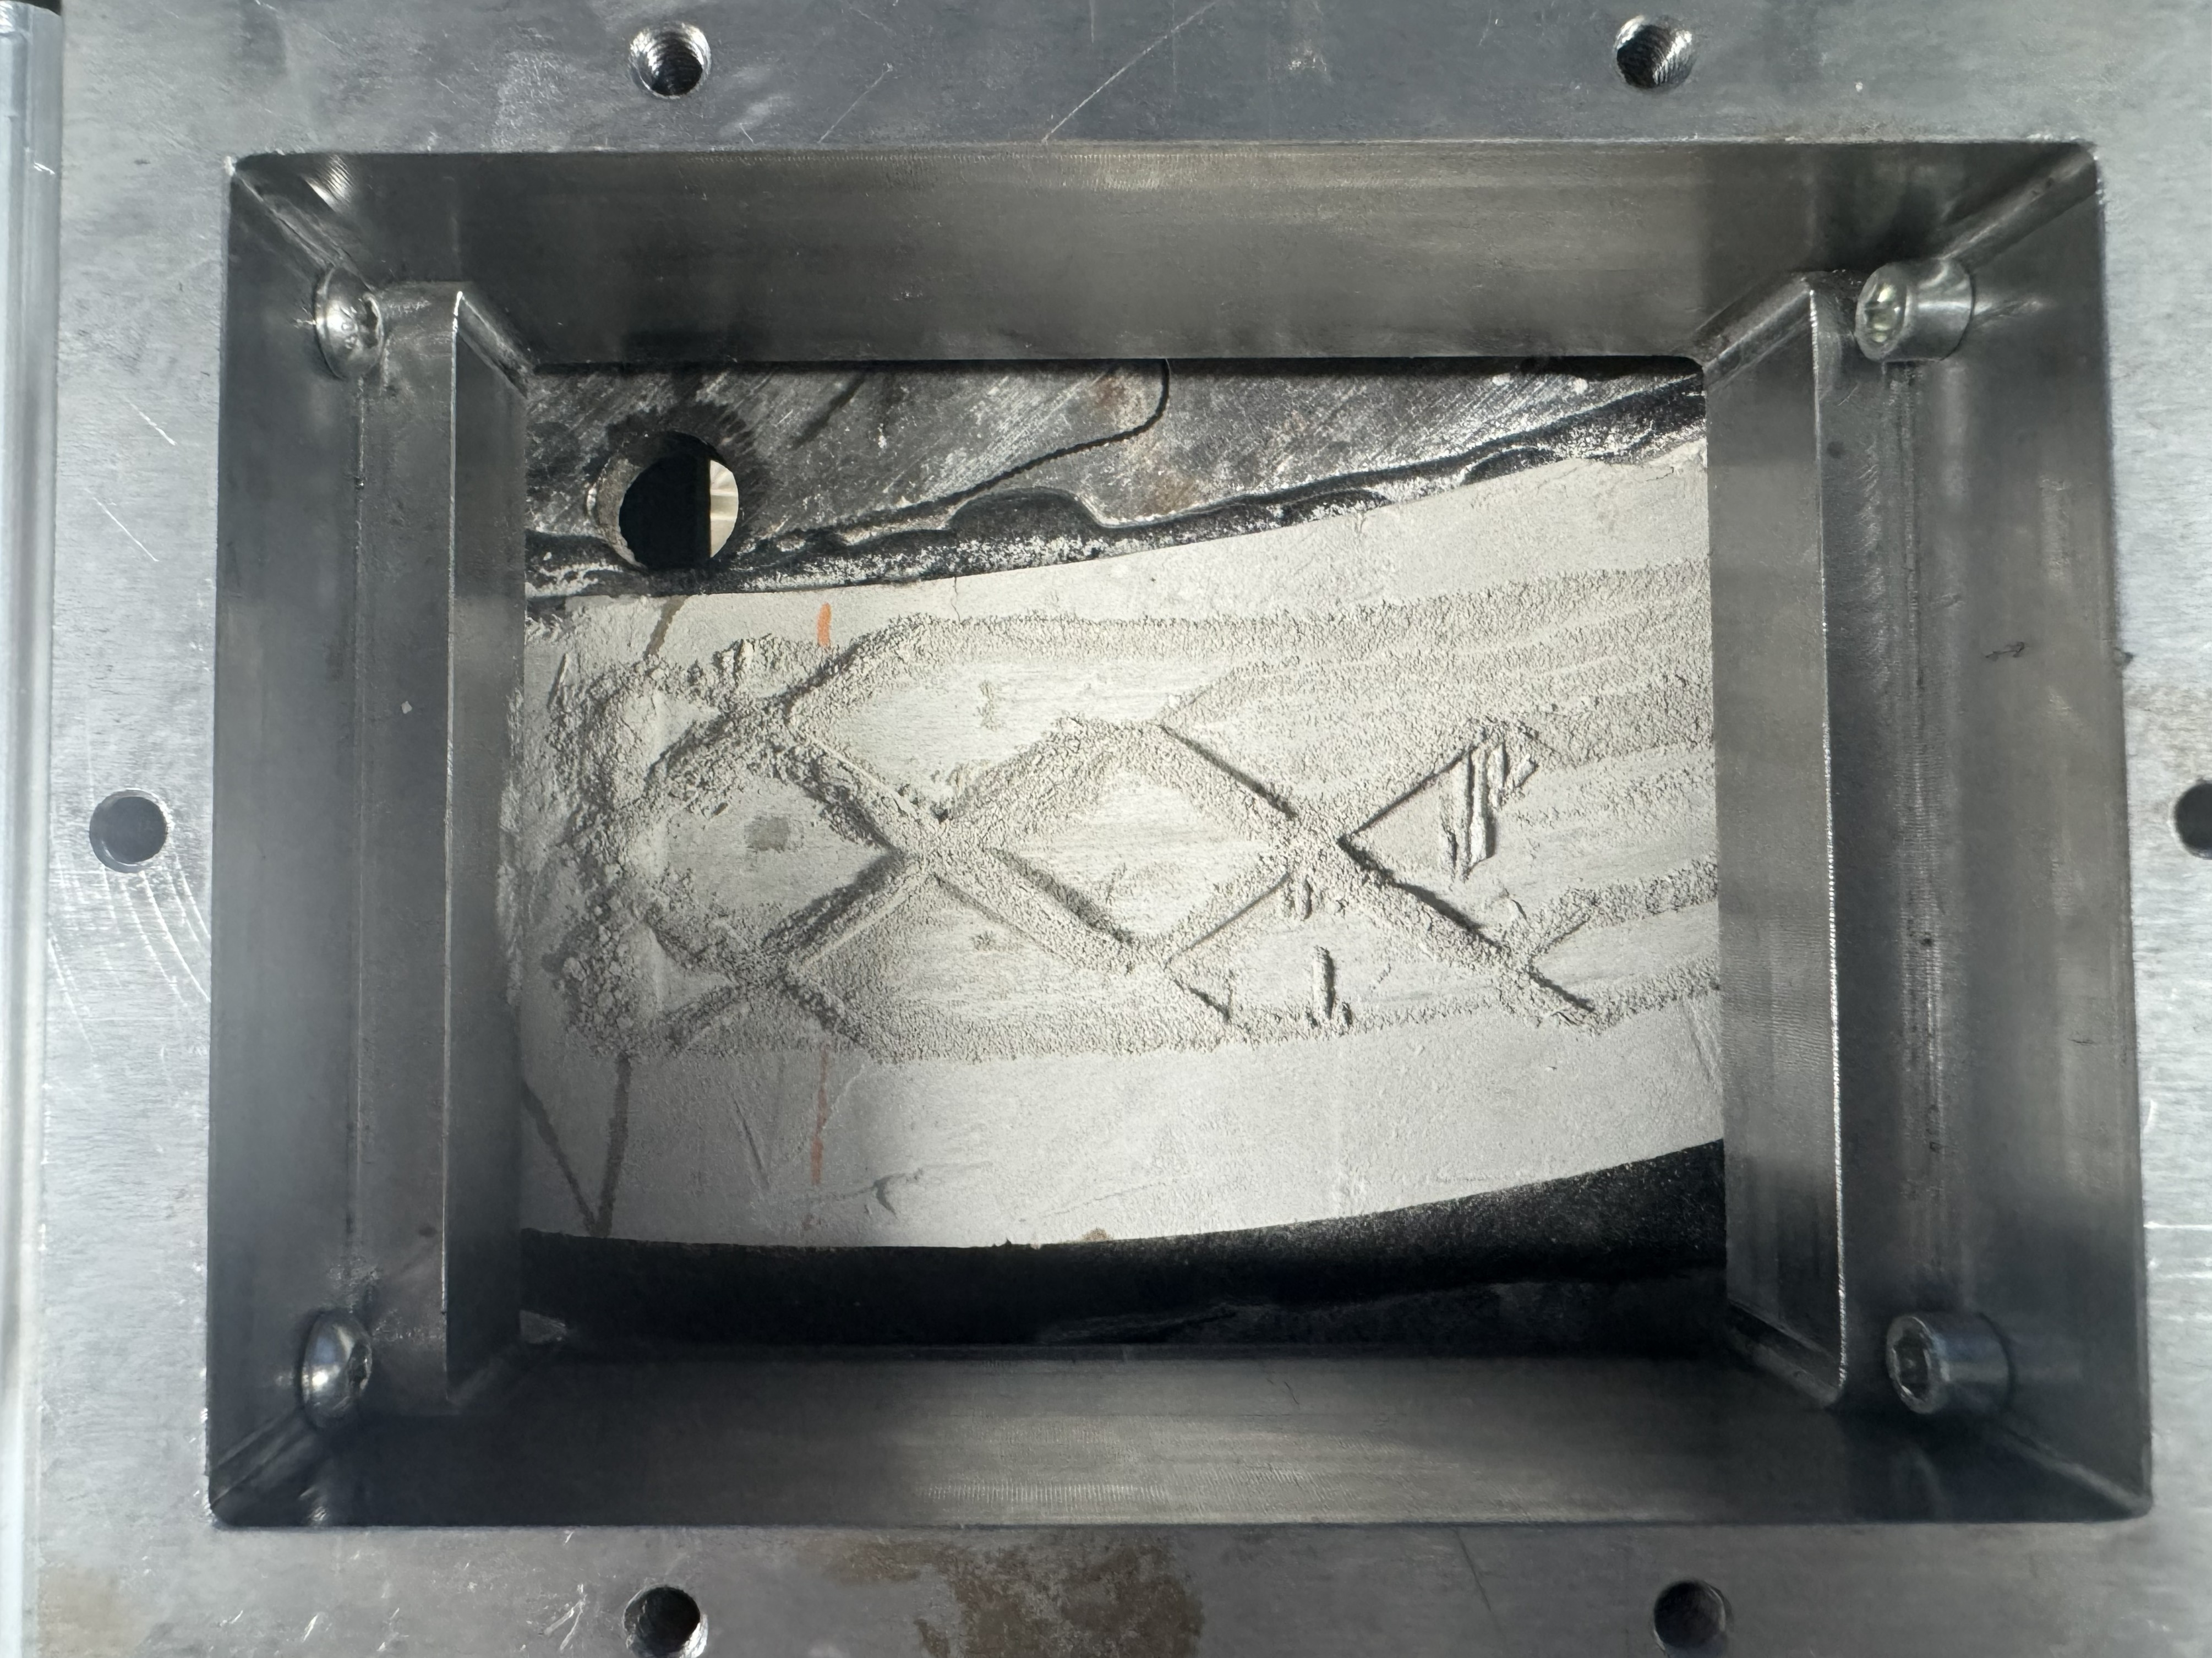
\includegraphics[height=4.0cm]{figure/chapter3/scale-4.jpg}
	\label{fig:scale_4}
	}
	\\[1.2em]
	\subfloat[$\delta_s=5.155\textrm{mm}$]{%
	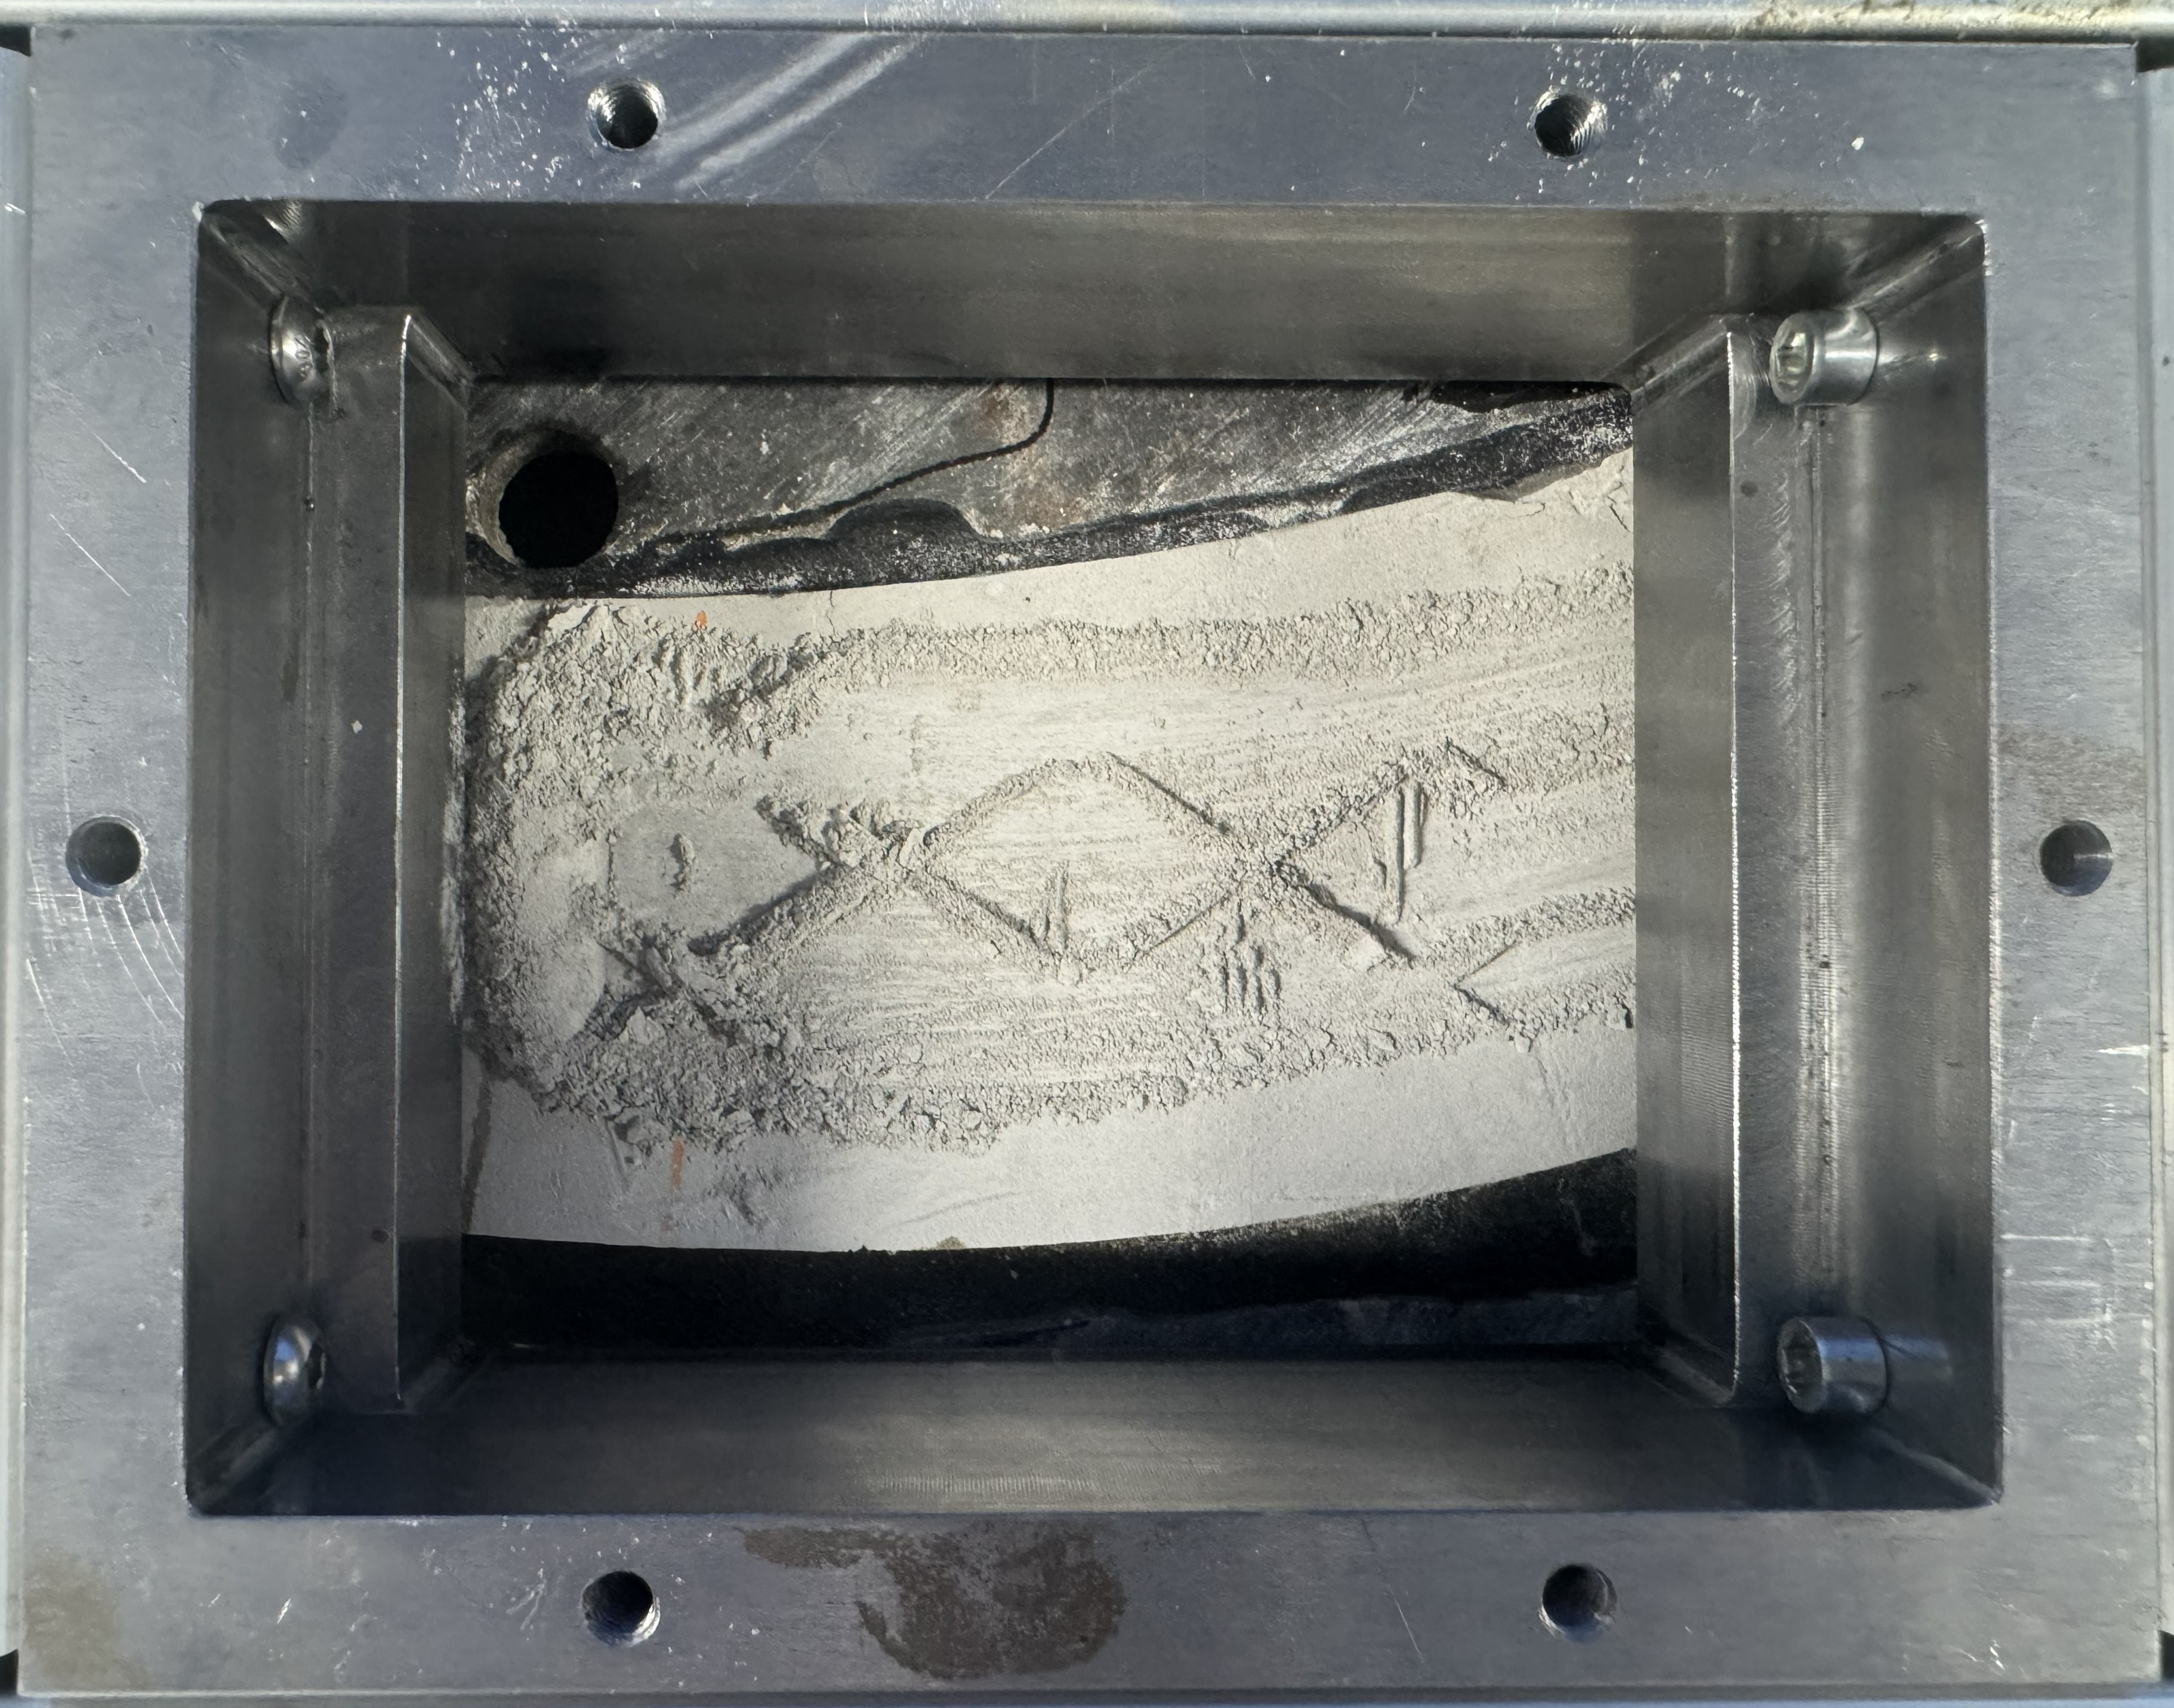
\includegraphics[height=4.0cm]{figure/chapter3/scale-3.jpg}
	\label{fig:scale_3}
	}
	%\hfill
	\subfloat[$\delta_s=6.465\textrm{mm}$]{%
	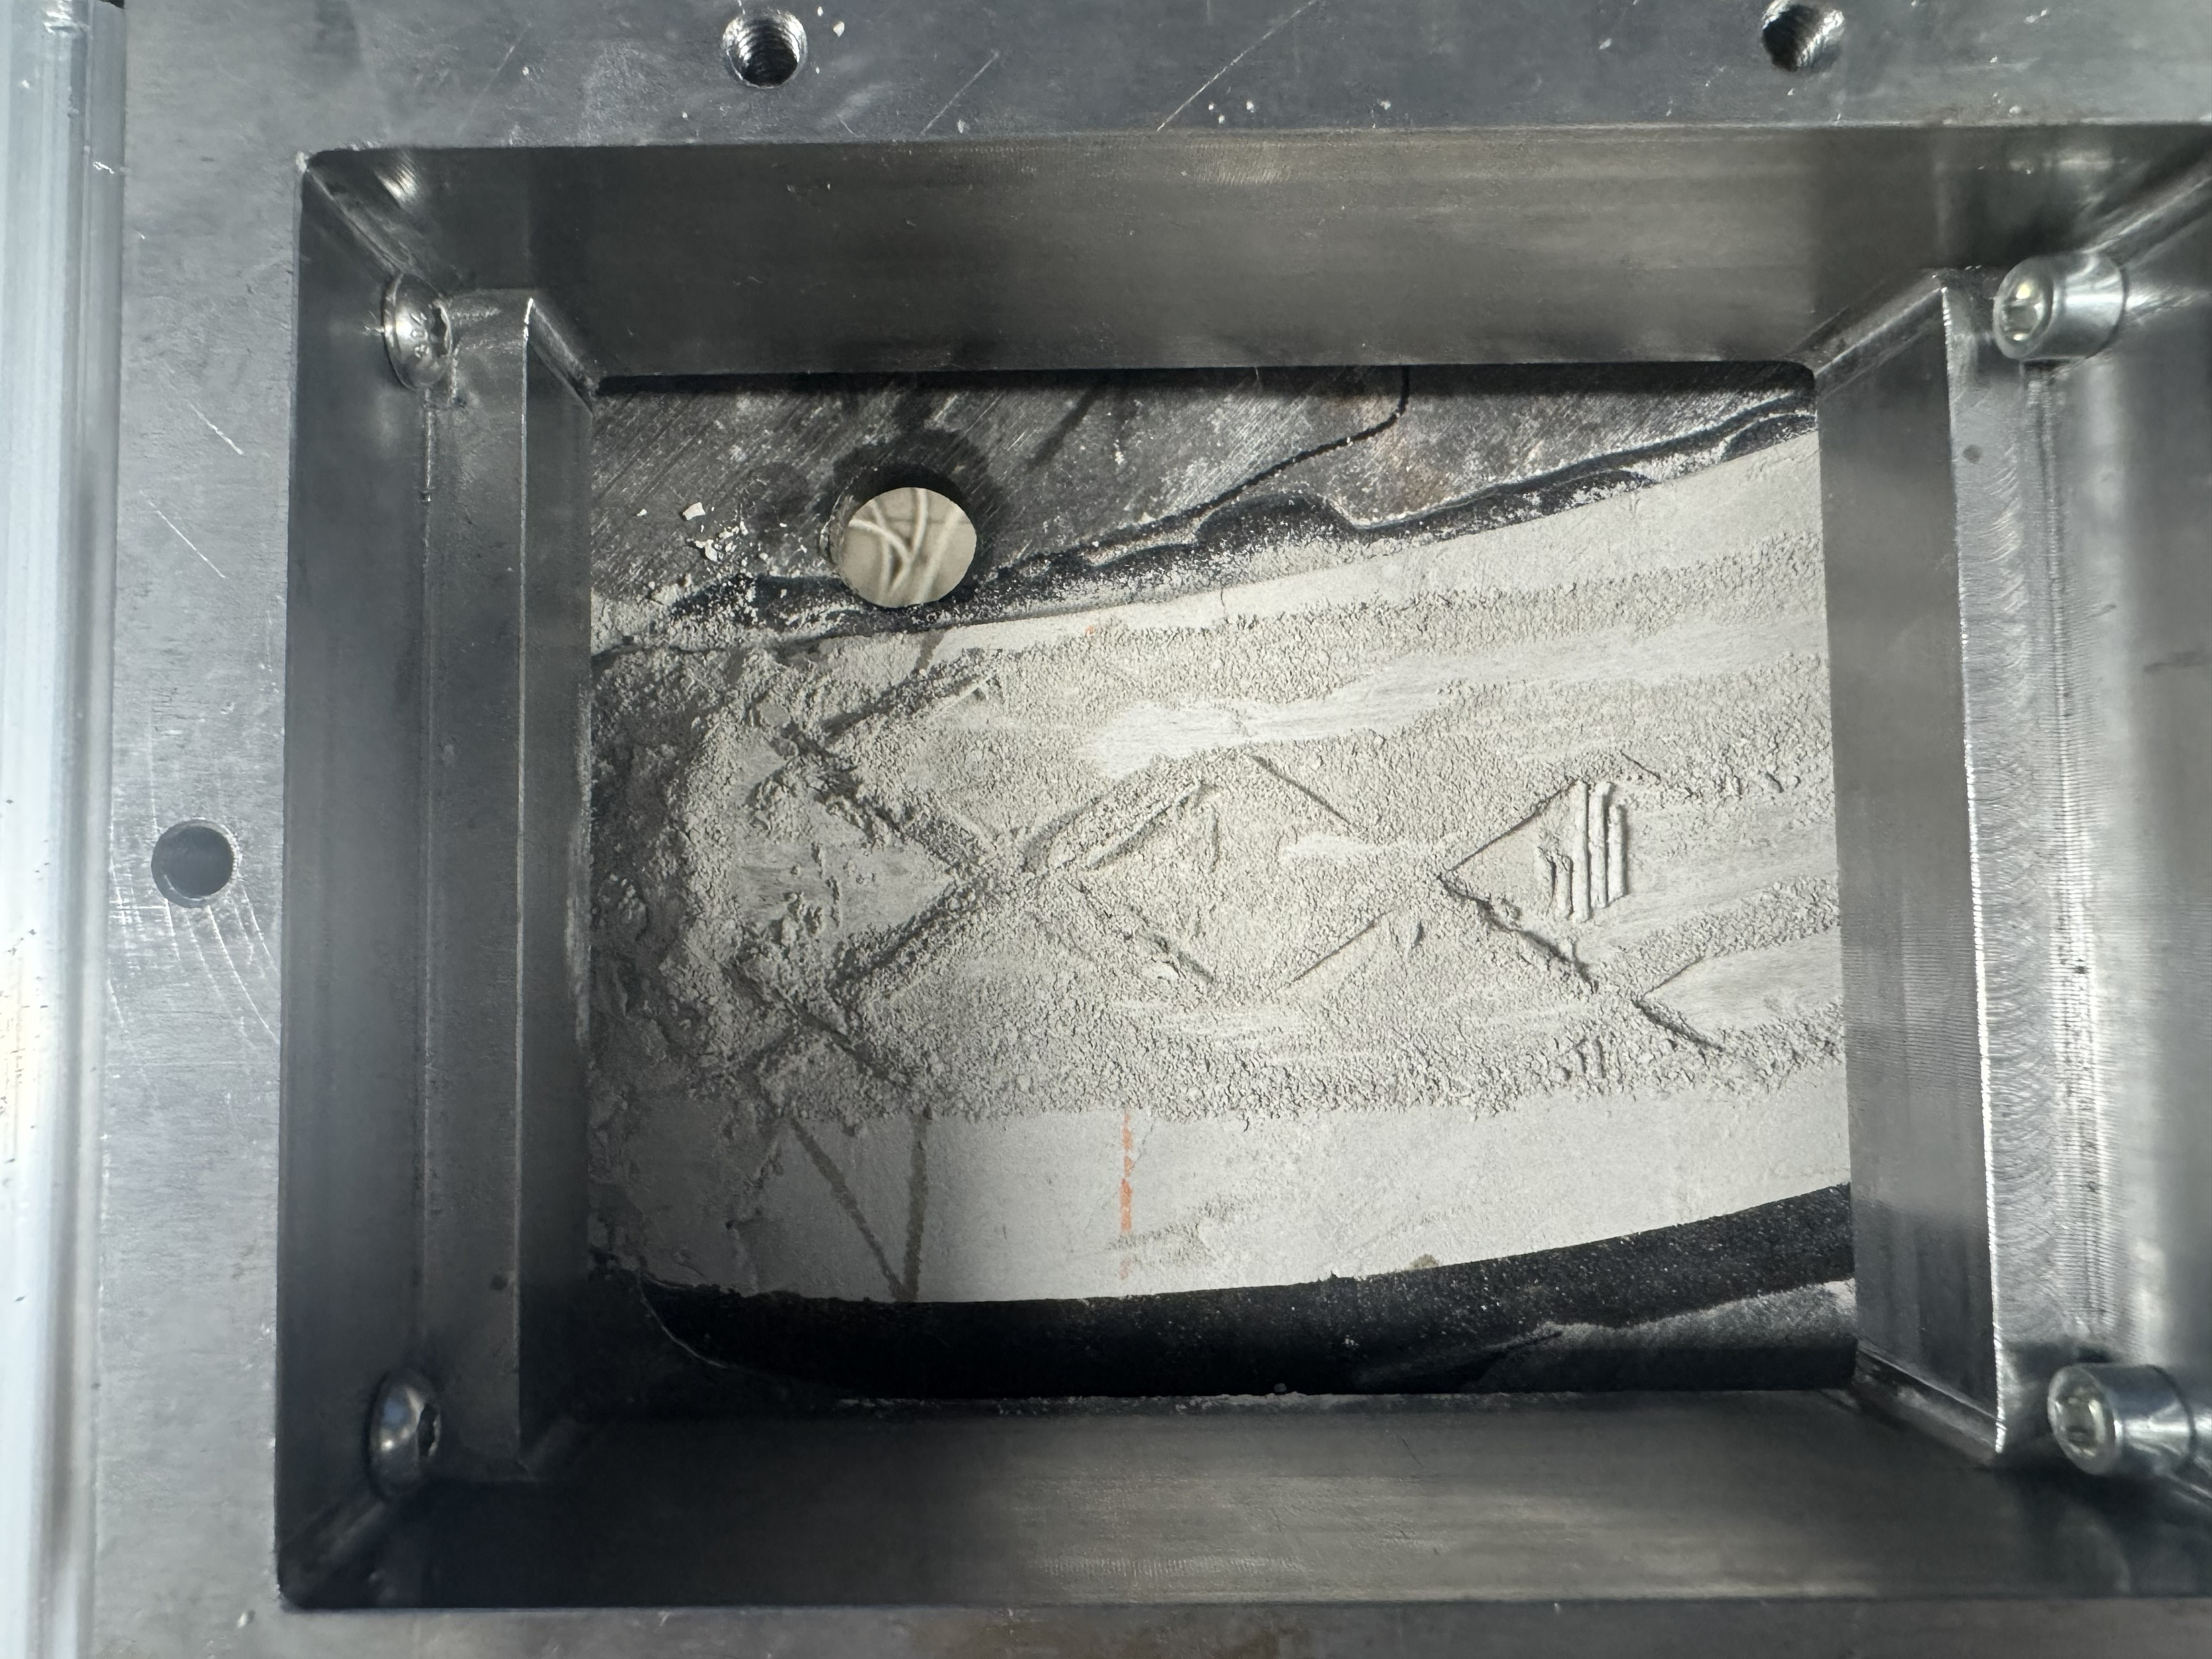
\includegraphics[height=4.0cm]{figure/chapter3/scale-5.jpg}
	\label{fig:scale_5}
	}	
	\caption{垢层经刮削后的表面形貌（不同弹簧压缩量）}
	\label{fig:scale_profile}
\end{figure}


此外，刮板表面的有效刮削功能单元是表面齿，总体上看，刮板主要依靠具有负前角的前刀面进行刮削，其余位置的齿起到辅助作用。刮削中产生的粉末状垢屑极易导致刮板上刀齿前刀面堵塞，如图\ref{fig:scraper_profile}所示。在清理垢时还发现，后刀面在弹簧的巨大预紧力作用下与垢强烈摩擦，后刀面附着有一层质地坚硬的垢变质层，其强度和硬度比垢基材高，在一定程度上减缓了后刀面的磨损。刮板前刀面附近的切削齿堵塞较为严重，增加弹簧的预紧力会加剧这种堵塞效果，这说明此刮板应容易堵塞。横向螺纹齿最容易被堵塞，斜向的三角齿由于容屑槽空间大，切削性能可保持的时间会更长。在实际应用中，可以推测，螺纹齿在刮削的初期就被堵塞而失效。主切削齿在初始阶段承担主要的刮削任务；随着刮削行程的增长，其主切削刃磨钝，三角齿主要起着刮削的作用。在实际应用中，如能建立循环不断冲洗刮板，将有助于屑从容屑槽中排出，对提高刮板的使用效能有促进作用。

\begin{figure}[htbp]
	\centering
	\subfloat[$\delta_s=3.095\textrm{mm}$]{%
	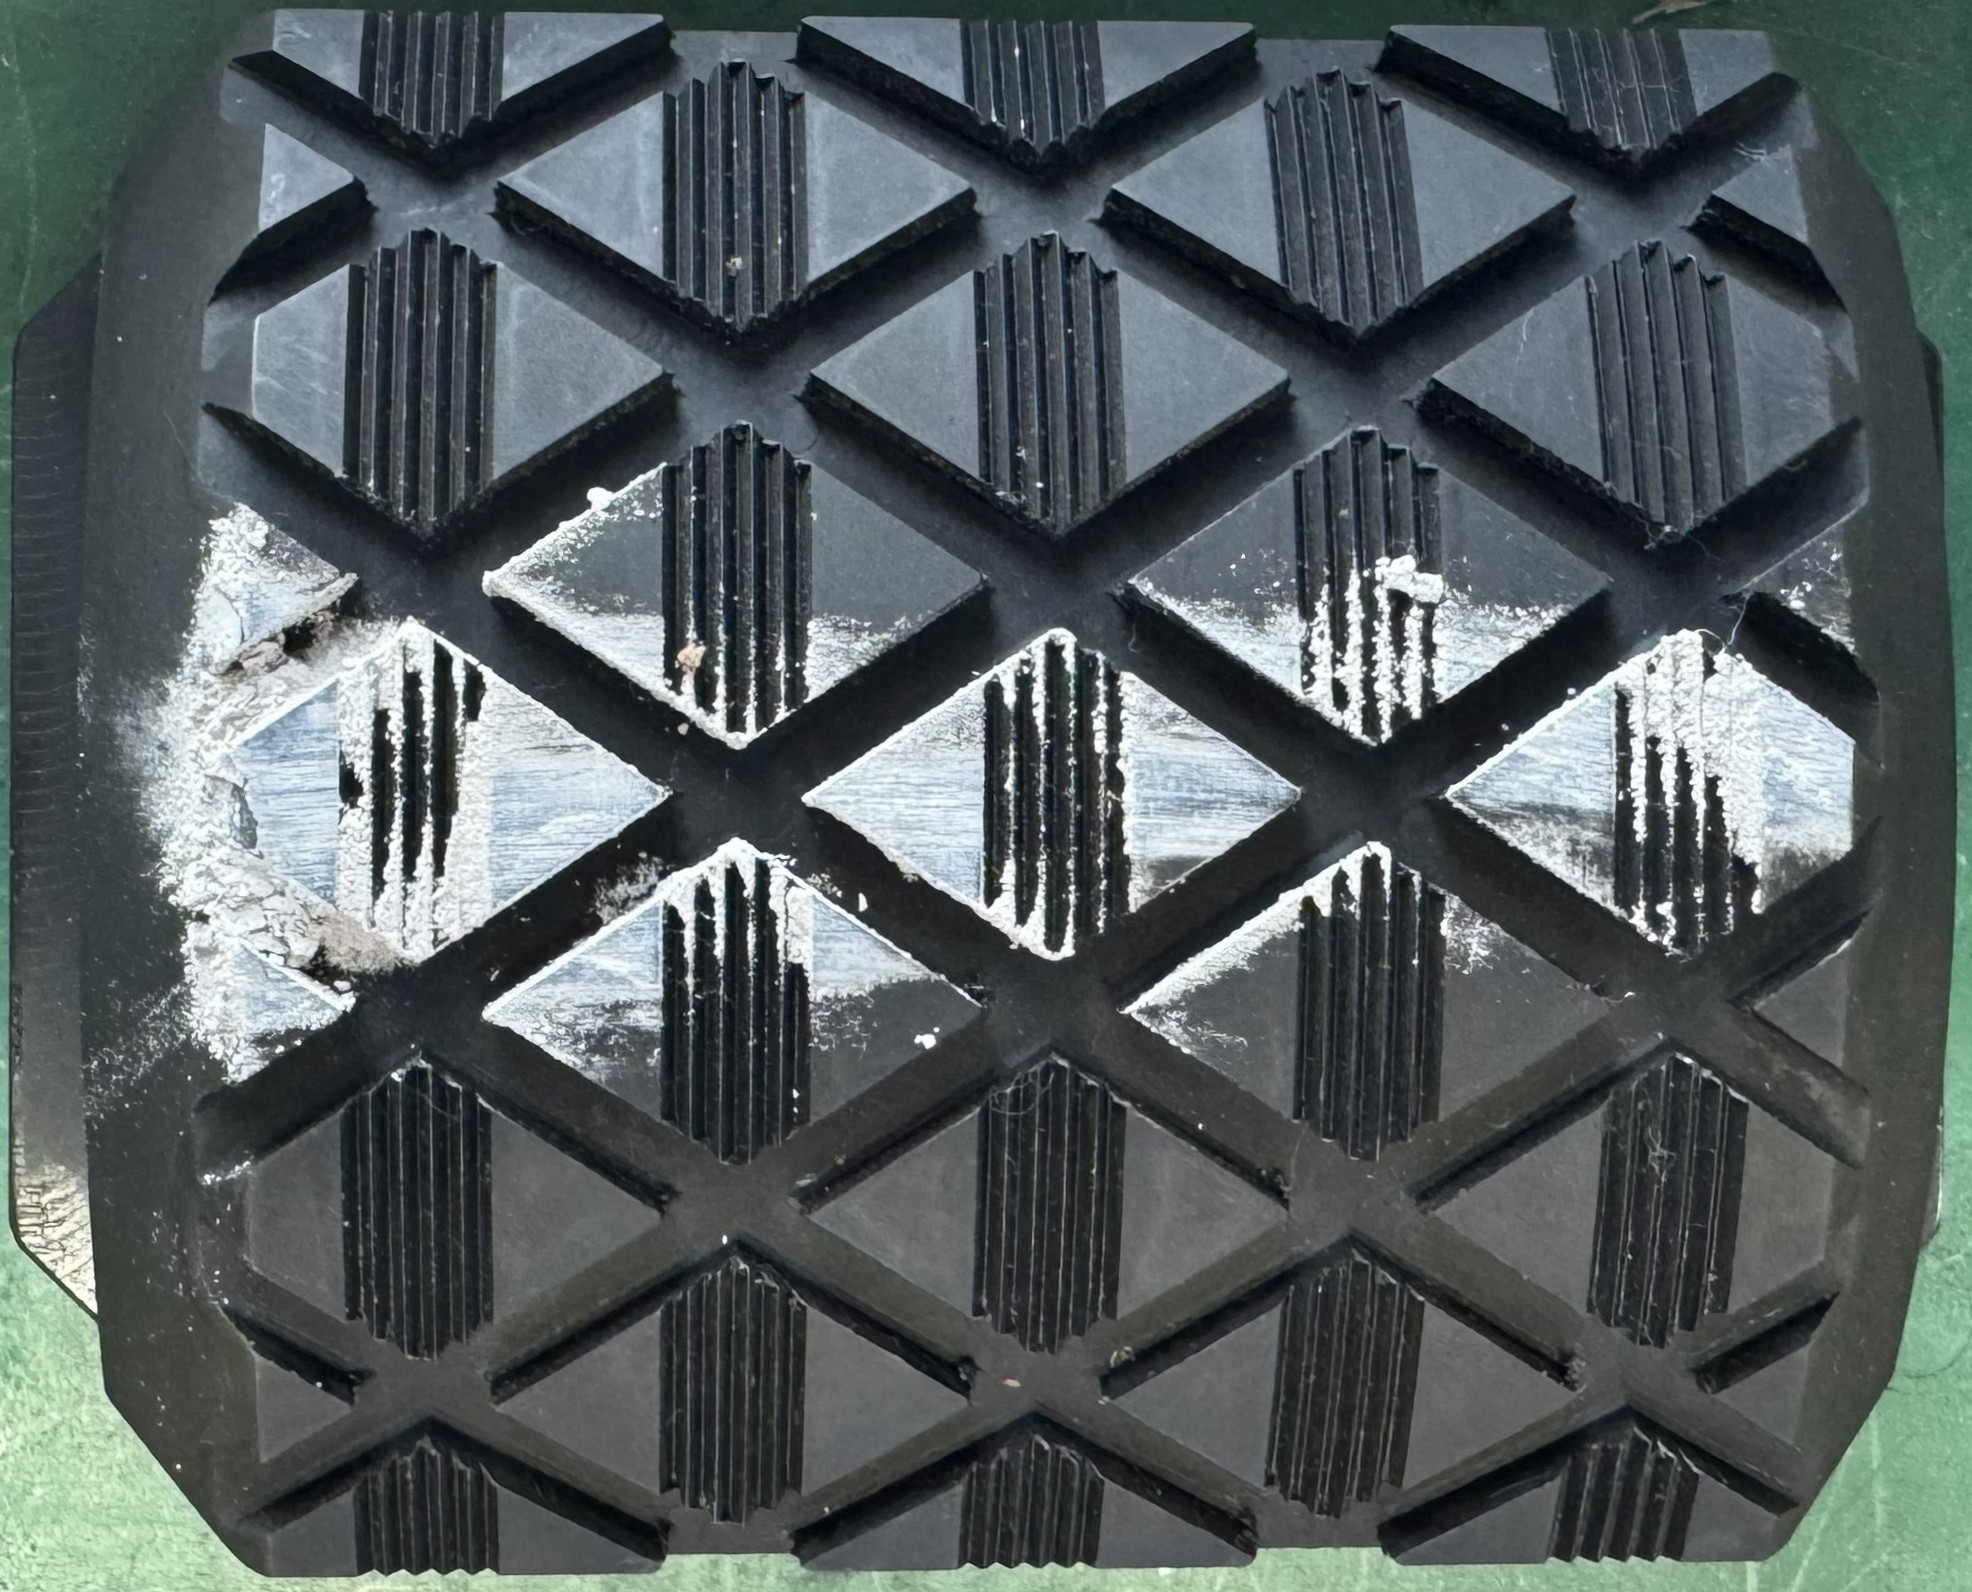
\includegraphics[width=.32\textwidth]{figure/chapter3/scraper-1.jpg}
	\label{fig:scraper_1}
	}
	%\hfill
	\subfloat[$\delta_s=4.875\textrm{mm}$]{%
	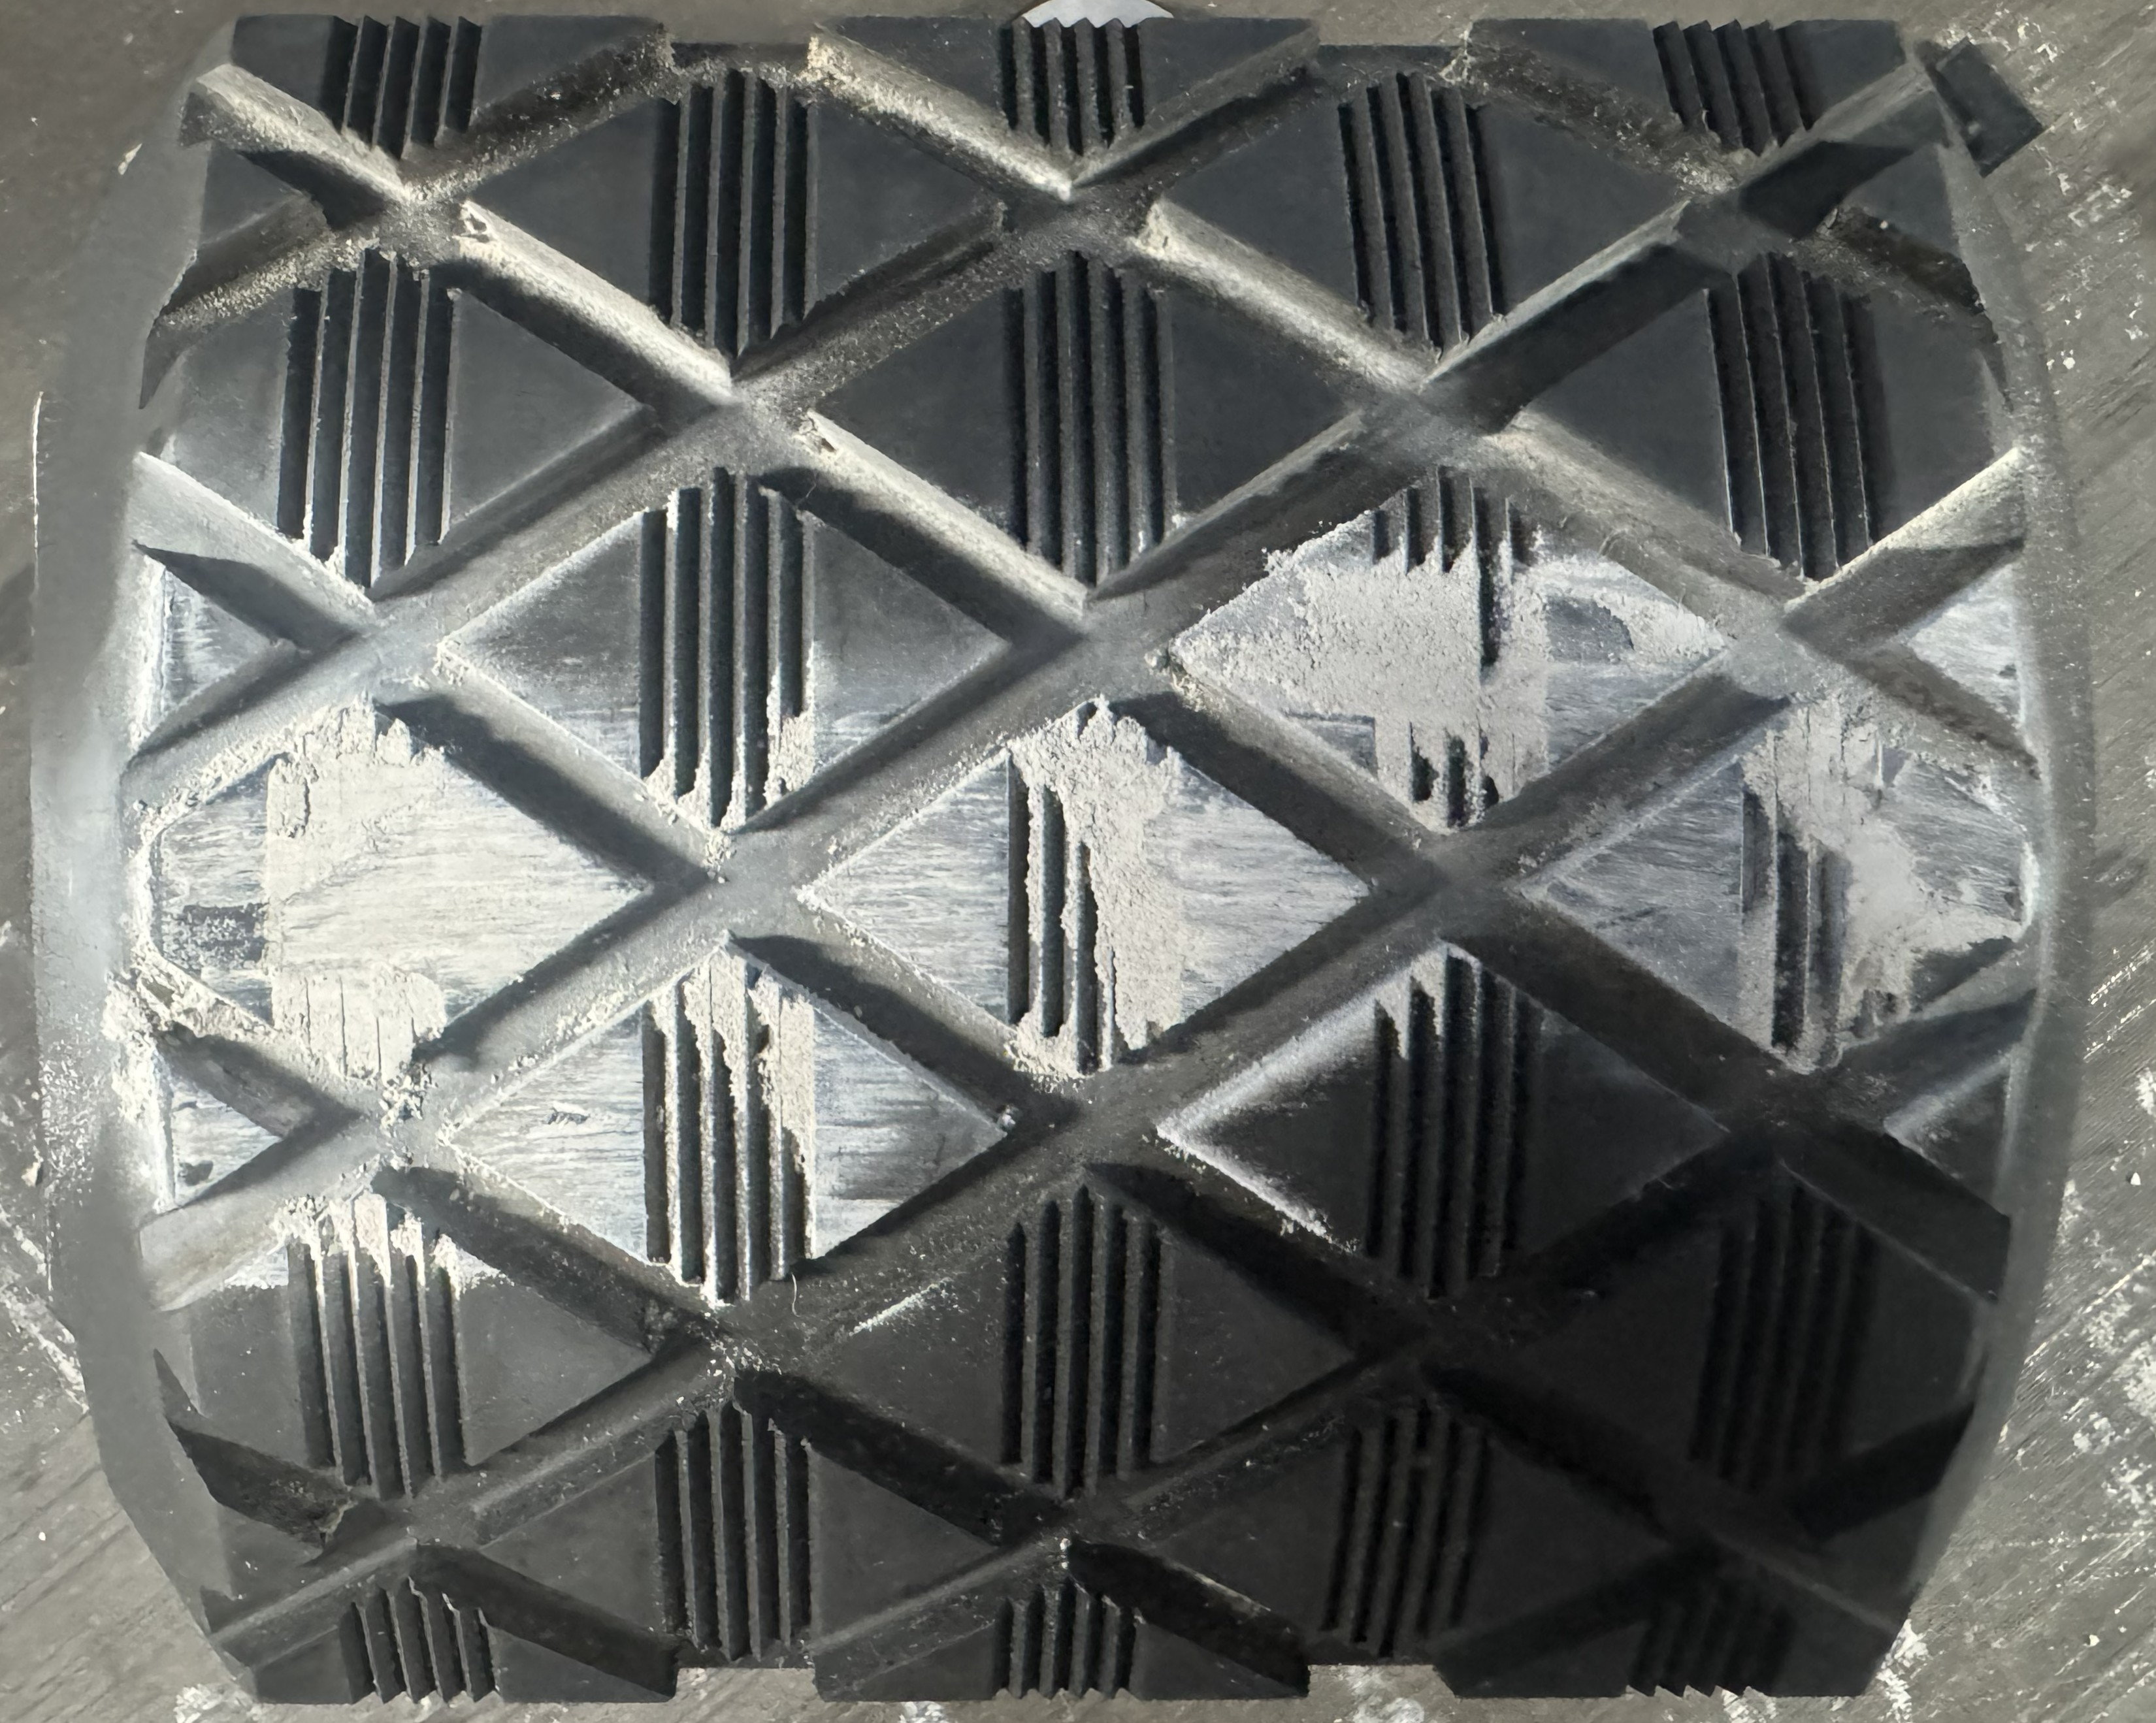
\includegraphics[width=.32\textwidth]{figure/chapter3/scraper-4.jpg}
	\label{fig:scraper_4}
	}
	\vspace{1em}
	\subfloat[$\delta_s=5.155\textrm{mm}$]{%
	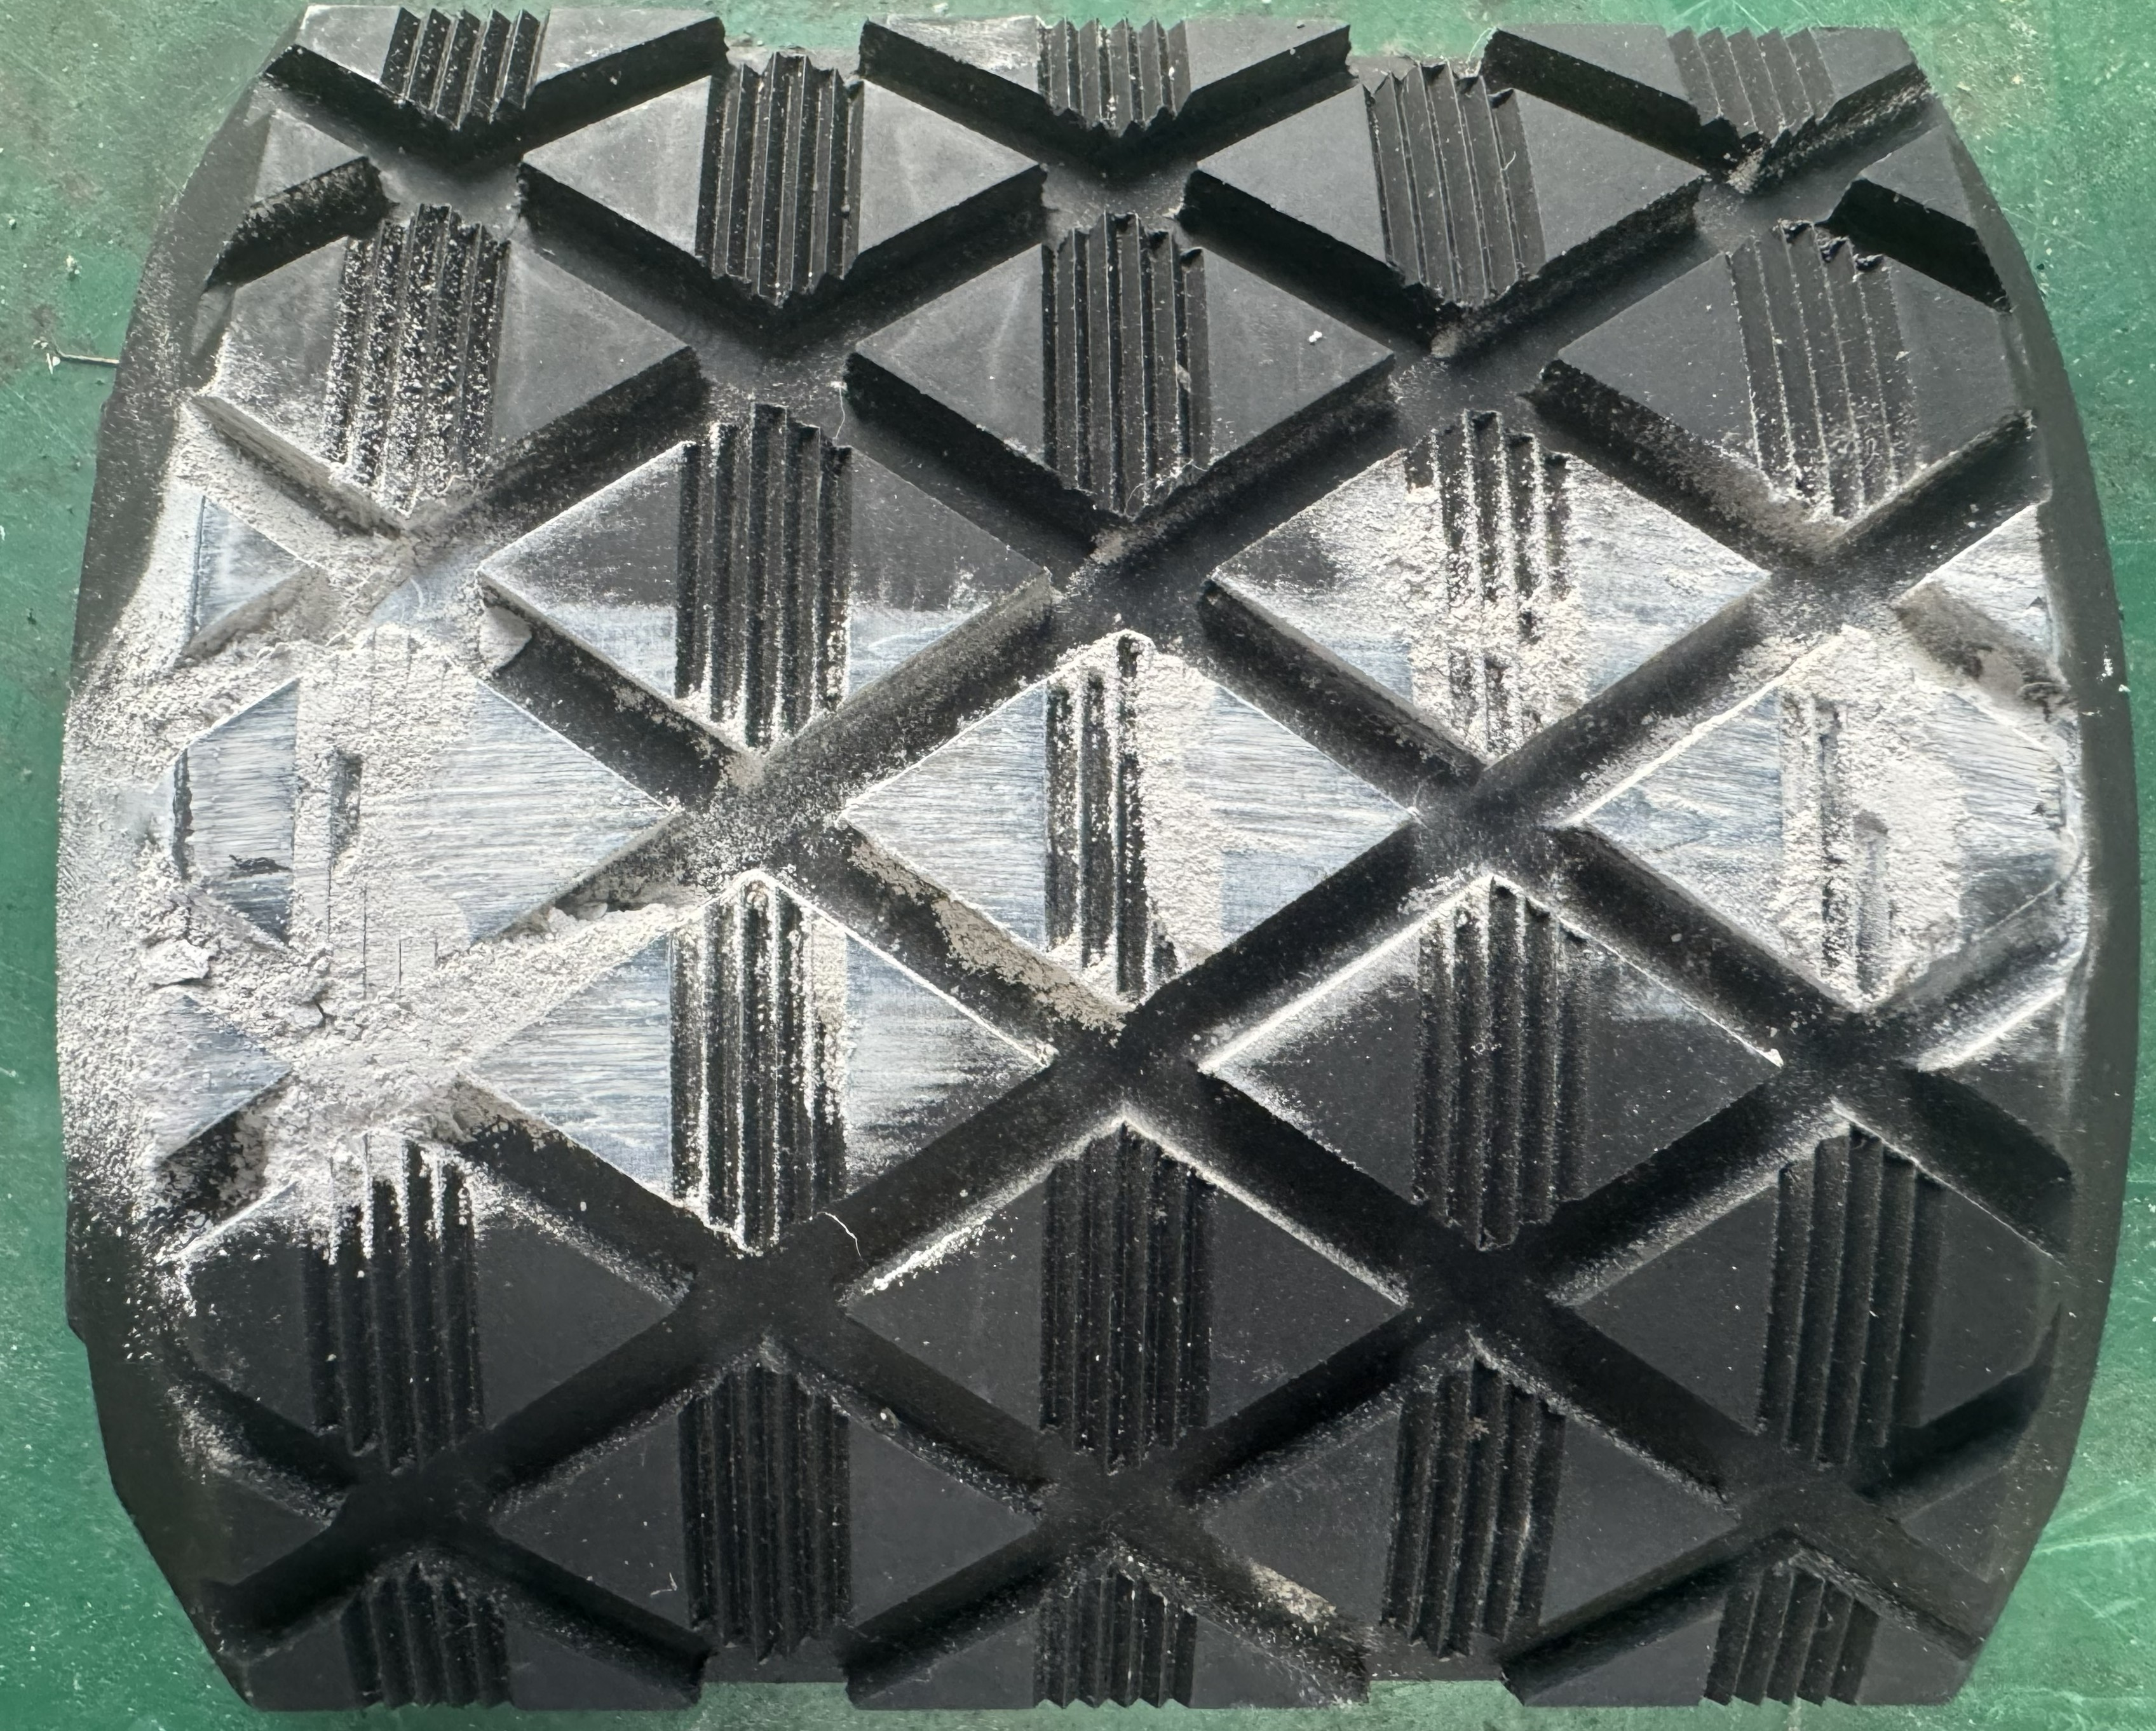
\includegraphics[width=.32\textwidth]{figure/chapter3/scraper-3.jpg}
	\label{fig:scraper_3}
	}
	%\hfill
	\subfloat[$\delta_s=6.465\textrm{mm}$]{%
	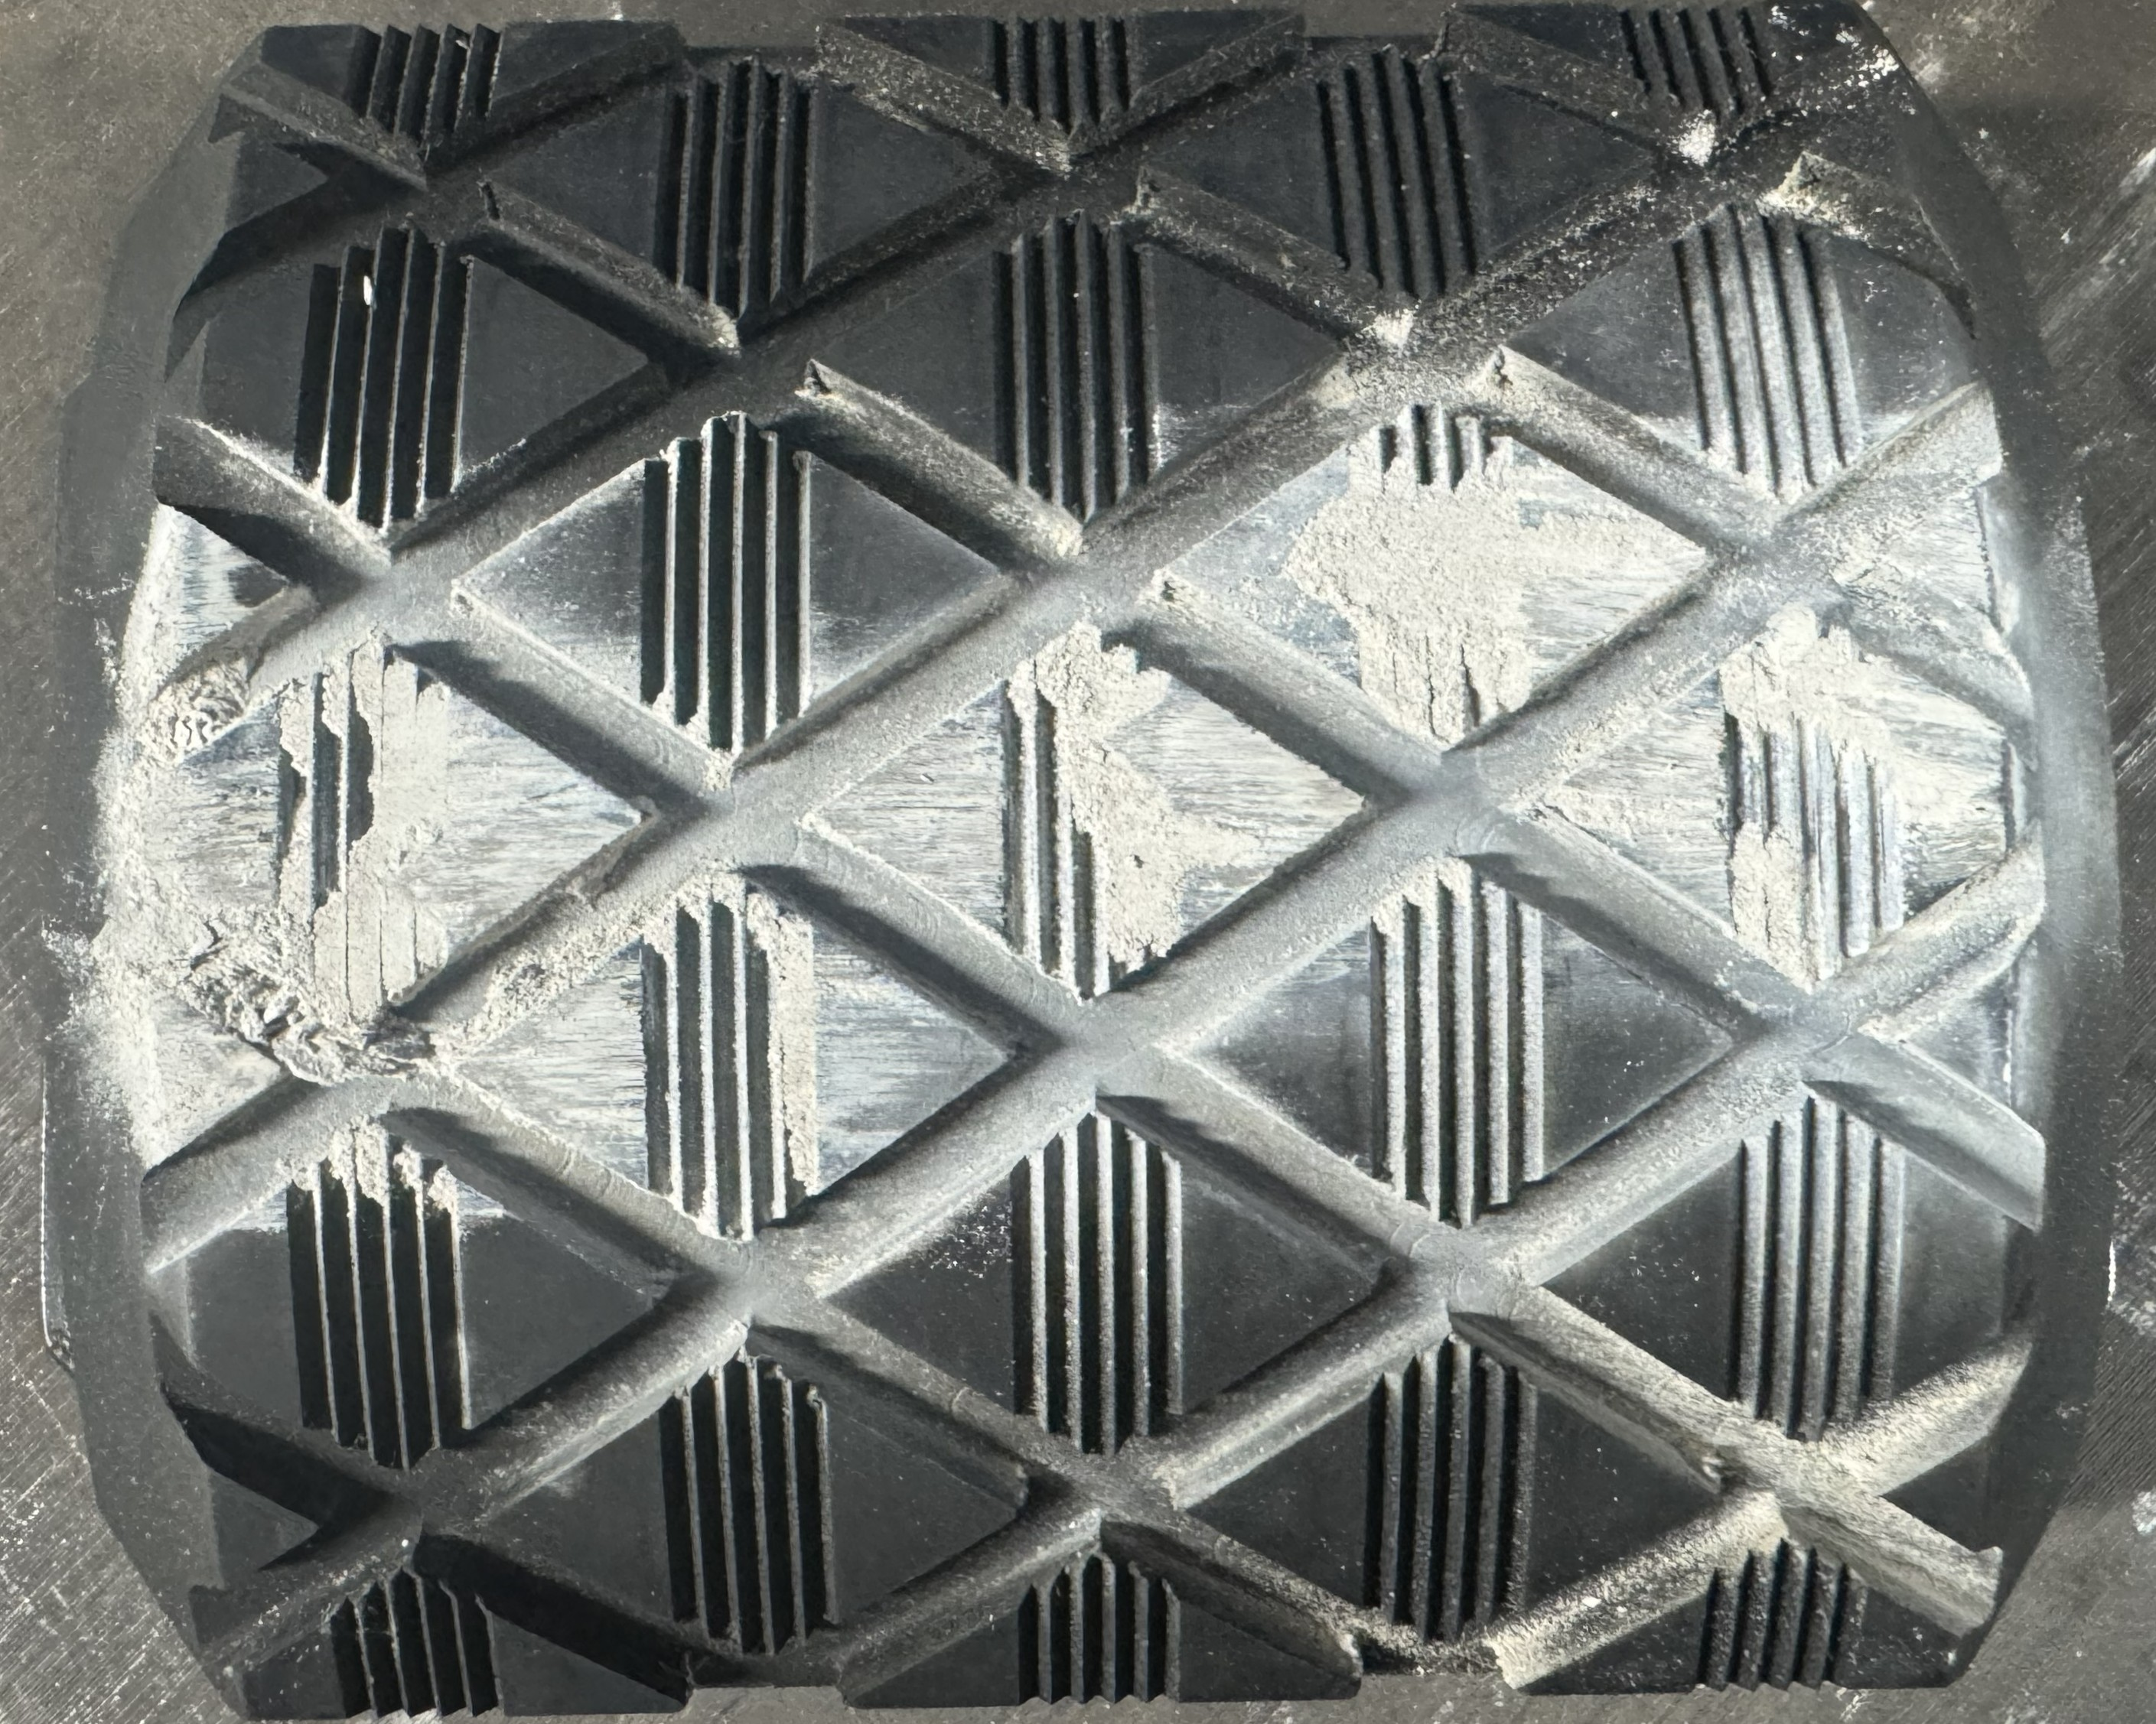
\includegraphics[width=.32\textwidth]{figure/chapter3/scraper-5.jpg}
	\label{fig:scaper_5}
	}	
	\caption{刮削后刮板刀齿表面形貌及切屑堵塞情况}
	\label{fig:scraper_profile}
\end{figure}



本试验基于图\ref{fig:scraper_test_rig}所示的转盘式台架，以重晶石粉与硫铝酸盐水泥配制的模拟硬垢为对象，考察了弹簧压缩量对刮板刮削效果的影响。结果表明：所设计的刮板能够有效刮除该类硬垢，但单次刮削厚度并不随弹簧预紧量的增大而增大，而是随弹簧压缩量的增大而减小，并在某一压缩量附近出现陡降，说明实际应用中弹簧预紧量存在临界值与有效工作区间。

从装置与方法看，转盘旋转可在低速条件下复现刮板相对垢面的刮削运动：接触区内相对运动方向与直线平动一致，线速度沿刮刀跨度虽有约±19\%的变化，但处于低速准静态范围，不改变硬垢脆性崩碎的去除机理；结合弹簧变形量与刮痕深度的逐点测量，可定量评价不同预紧工况下的刮削效果，为刮管工具的台架评价提供了可行方法。

从刮削形貌看，刮削后的垢面呈连续规则的沟槽，刀齿前刀面与容屑槽内见粉末状及崩碎状切屑（图\ref{fig:scale_profile}），表明垢层以脆性崩碎方式去除，刮板具备对重晶石/钡锶类硬垢的实际刮除能力；同时可见，产屑量随弹簧压缩量的增大而增多，而细屑对刀齿前刀面、容屑槽的充填堵塞及垢面压实变质层的发育也随压缩量的增大而加剧（图\ref{fig:scraper_profile}），说明单纯增大预紧量并不能成比例地提高有效刮削能力，这与图\ref{fig:scratch_depth_spring_comprassion}所示的响应规律一致。

从单次刮削厚度随弹簧压缩估计值的响应看（图\ref{fig:scratch_depth_spring_comprassion}），二者并非单调递增关系，而呈“缓降—陡降—稳定”的三段特征：弹簧压缩量约为3.9 mm和5.5 mm时，单次刮削厚度分别约为0.85 mm和0.71 mm，降幅不大；压缩量增至约7.1 mm时，厚度约为0.64 mm；压缩量进一步增至约7.3 mm时，厚度骤降至约0.11 mm；此后（约9.6 mm）厚度基本稳定在0.08 mm左右。由此可知，弹簧预紧量存在临界值（本试验条件下约为7.2 mm）：在临界值以内，刀齿能够保持相对稳定的压入深度，单次刮削厚度随压缩量的增大缓慢减小；当压缩量接近并超过临界值后，一方面刀齿与垢面的实际接触面积显著增大、垢层表面被压实变质并产生大量细屑，细屑迅速充填刀齿前刀面与容屑槽（图\ref{fig:scraper_profile}），参与有效切削的齿减少；另一方面刮板的浮动支撑逐渐接近其径向行程极限，刀齿难以继续压入垢层，刮削中切削所占比重下降、挤压与摩擦所占比重上升，单次刮削厚度急剧下降并趋于稳定。需要说明的是，本文各工况在同一扇形垢样、同一沟槽上依次进行，弹簧压缩量随工况逐步调整，图中反映的是弹簧压缩量对刮削厚度的总体影响趋势。

面向工程应用，弹簧预紧量不宜盲目加大，而应控制在其有效区间内：预紧量过小，刀齿难以始终贴紧壁面，清洁能力受限；预紧量过大，单次刮削厚度不升反降，并会因齿面堵塞和浮动支撑压死使刮削能力骤降，同时加剧刀齿与后刀面的磨损。按本节试验结果，弹簧压缩量在约4$\sim$7 mm范围内时，单次刮削厚度保持在较高水平且变化平缓，可作为该刮板预紧量的推荐工作区间；实际应用中还应结合套管的实际内径（同一公称尺寸不同线重时内径不同）匹配刮刀外径与弹簧预紧量，使弹簧压缩量不超过临界值，避免盲目增大预紧力；现场作业宜配合循环冲洗及时排屑，以延缓齿面堵塞、延长刮板有效使用寿命。

综上，研制的刮板对重晶石/钡锶类硬垢刮削有效，转盘台架及其测量方法可用于刮板刮削能力的相对评价；单次刮削厚度随弹簧压缩量的增大而减小，并在约7.2 mm附近出现陡降，说明弹簧预紧量存在临界值，实际应用中应结合套管规格匹配刮刀外径与弹簧预紧量、将弹簧压缩量控制在临界值以内，并辅以循环排屑措施。
\begin{figure}	
	\centering
	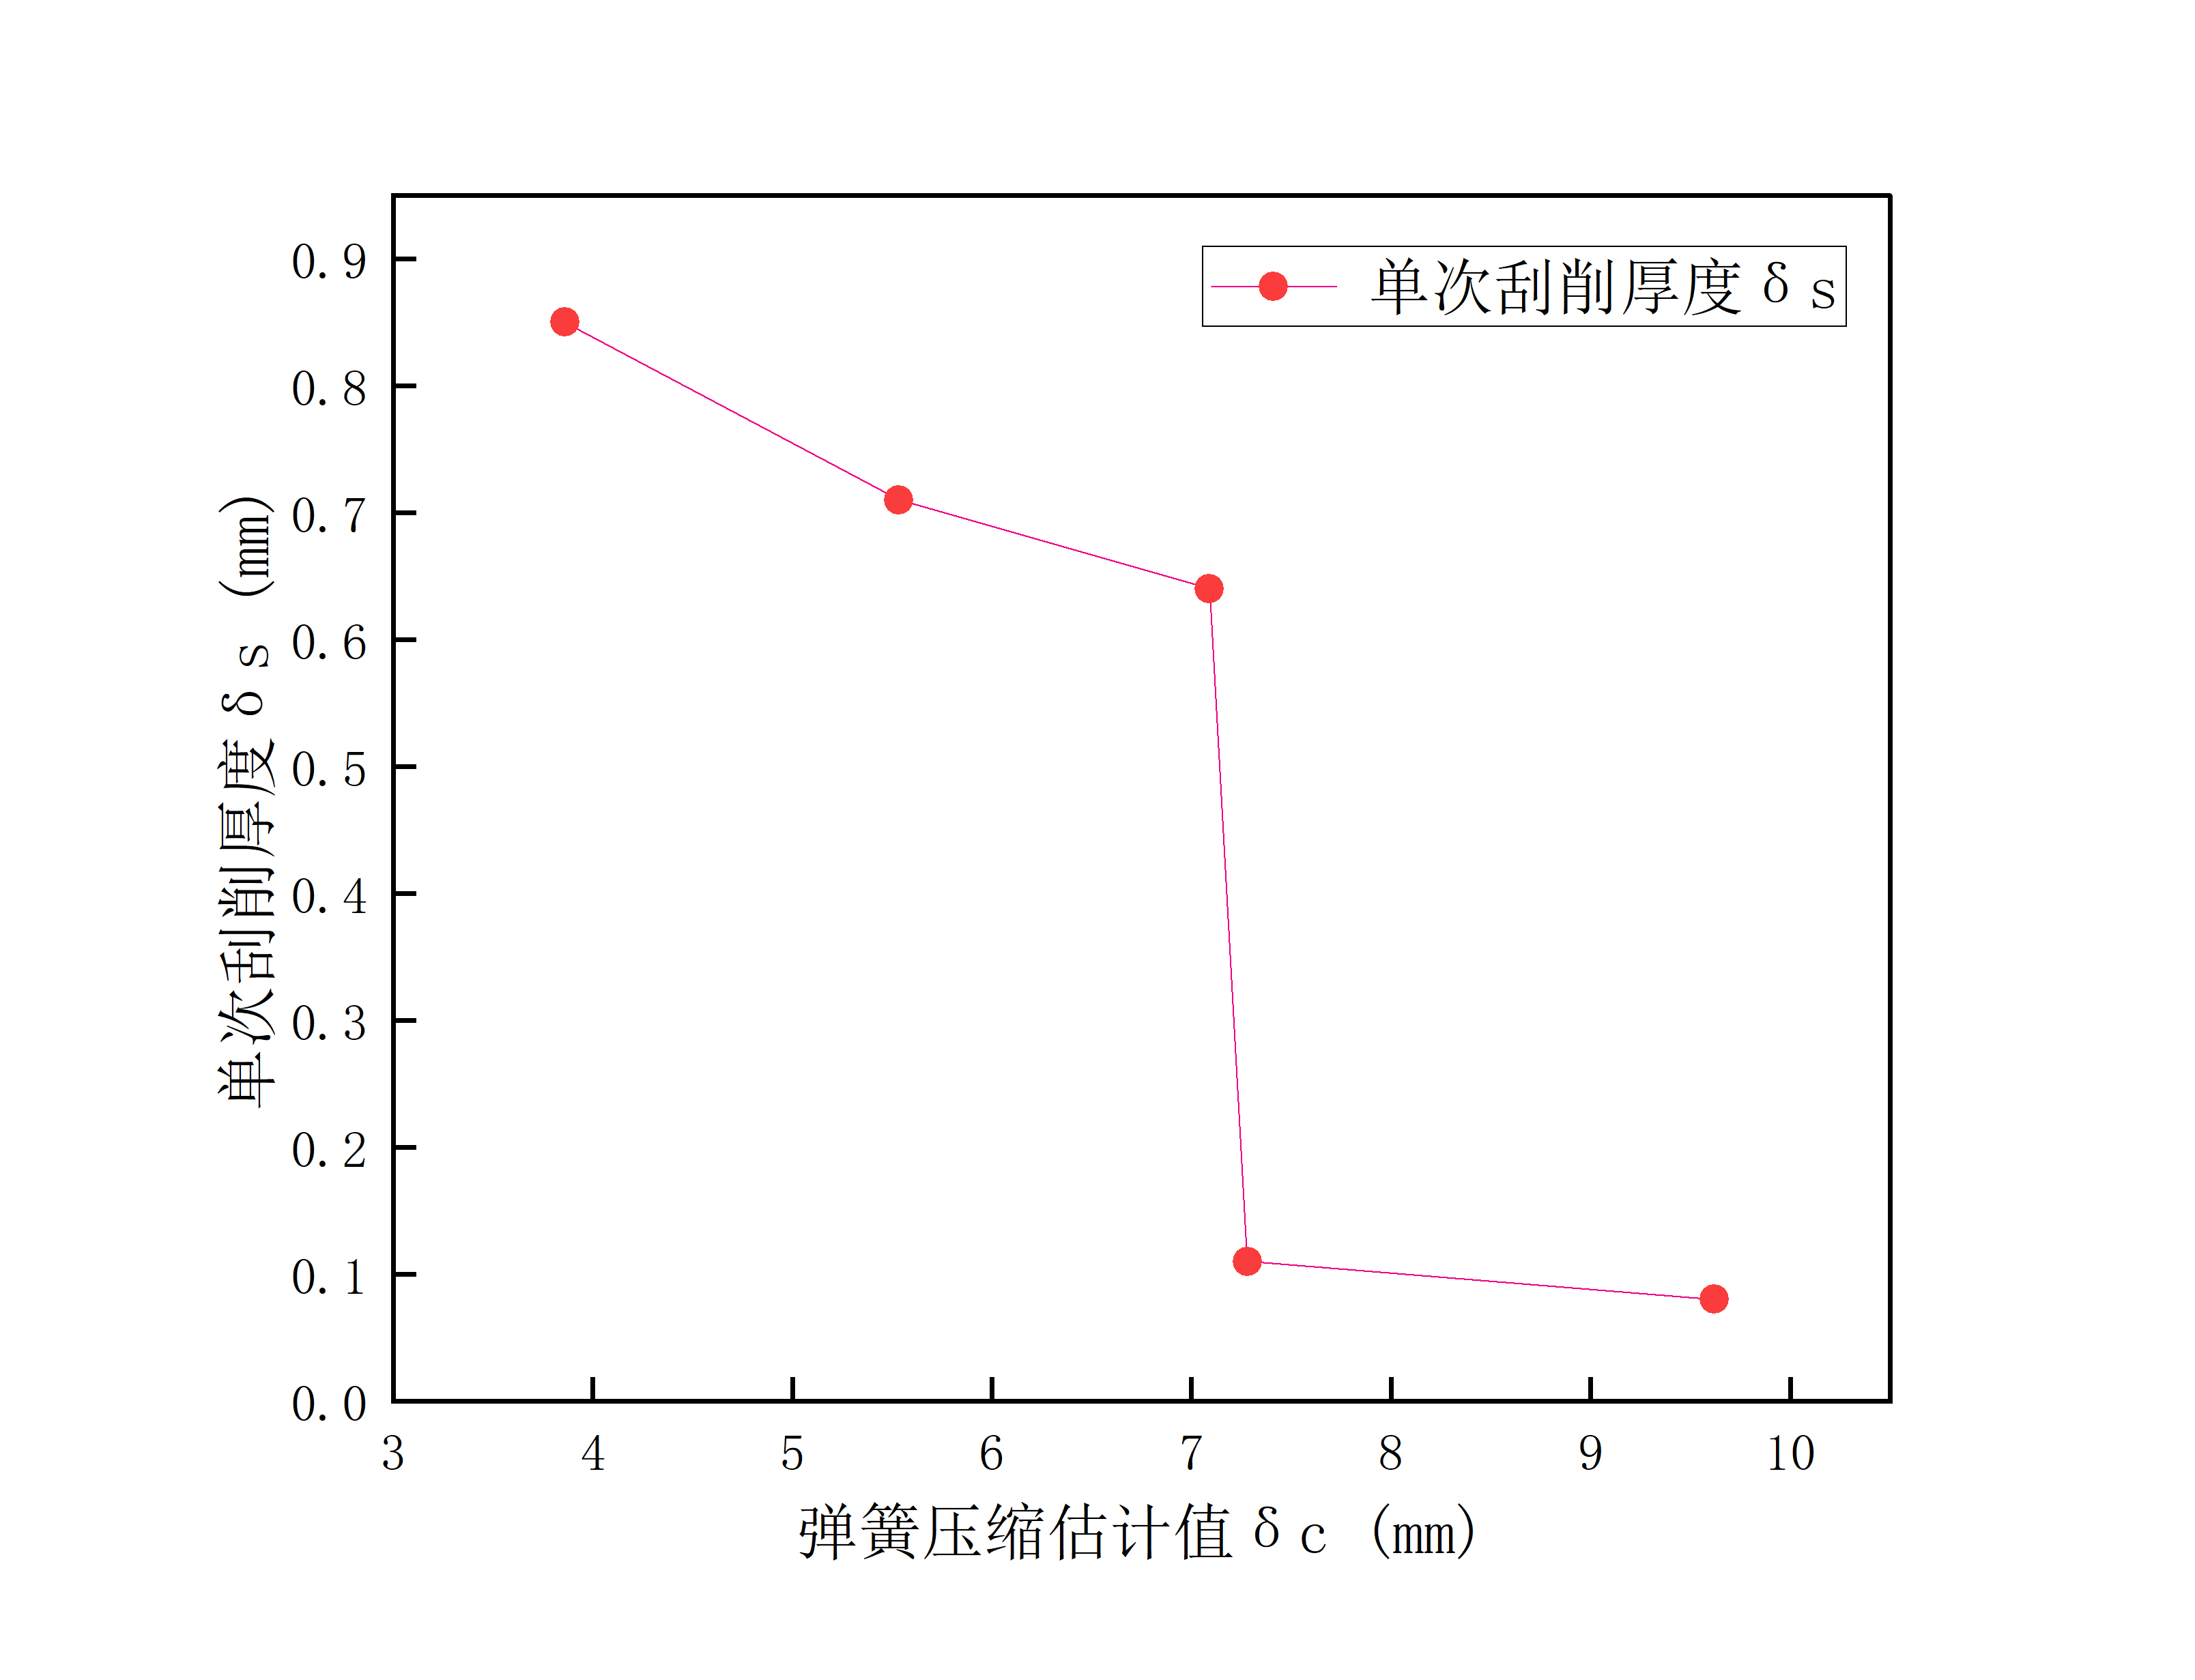
\includegraphics[width=.7\textwidth]{figure/chapter3/scatch-depth-sping-comprassion.jpg}
	\caption{刮削深度与弹簧压缩量之间的关系}
	\label{fig:scratch_depth_spring_comprassion}
\end{figure}


%\subsection{毛刷刮削力学仿真}


\subsection{操作方式}
\subsubsection{ 使用方法}
根据井眼尺寸选择合适的套管清洁工具，根据井眼情况选择各模块的数量及排列组合方式。
四合一工具用钻柱送入井底进行清洁作业。
\subsubsection{ 操作方法}
该工具可以与强磁吸附工具一同使用（推荐），也可以单独使用。
将四合一工具下到井底离通井位置$\mathrm{3-5m}$处，开泵循环。将四合一工具在该位置上下活动。保持循环的情况下，平稳的上体钻柱。
起钻时要求平稳、低速、严禁剧烈震动与撞击。

\subsection{维护与保养}
\subsubsection{保养}
下井使用过的四合一工具必须进行保养及维修，在钻台现场进 行保养是在井场钻台上起出井后，四合一工具外表面和水眼内的泥浆。

\subsubsection{管子站维修}
建议：在井下正常运转400小时后的四合一工具应送管子站进行大修，必须更换所有密封件和易损件，工具大修三次后报废。外筒零件磨损量（或偏磨量）大于产品外径尺寸1\%时，该套管清洁工具报废。修前应准备好下列设备、工具、附件：适用于该工具尺寸的链钳、管钳、手钳等相应工具；起重吊车、固定钳、稳定座、拆装架，试验架等设备；清洗用的煤油等；各种所需的润滑脂、润滑油等。

\subsection{测试与检查}

刮削器所用金属材料如需作力学性能试验，应按GB/T228的有关规定进行。刮板寿命按照SY/T 5110-2000进行刮刀寿命测试，刮削器的刮削寿命试验应在模拟试验台上进行。选用500号硅酸盐水泥，在对应的试验套管内壁上候凝24h。将试验套管固定在试验台底座上，将刮削器接到试验台的钻杆上，加压力$0.8~10\mathrm{kN}$，用$36\mathrm{r/min}$的速度进行模拟刮削，每次刮削1h，刮削3次。然后拆检测量刀体的磨损量，用渐进法验证其寿命。

四合一工具拆卸后应尽快进行检查，更换不满足使用条件的配件，不能采用非原厂配件。清洗前的检查，肉眼检查外部零件的损坏并记录异常磨损或作记号。如果发现明显损伤，需要对配件进行特别处理。清洗，用水浸泡零件以除掉干的结块和泥浆。用蒸汽和强力生物清洁剂去掉油和黄油。配件干燥、冷却后进行检查。

每次套管清洁工具被拆开时，用下述步骤检查所有配件。按API标准检查所有的接头螺纹，检查步骤要符合API标准。检查所有的配合面和端面是否清洗和磨损，需要时，修理和更换配件。检查所有外部配件是否磨损，当外径磨损超过尺寸的1\%以上时， 更换配件。配件有超过最小磨损量的凹槽或缺口不能继续使用，在一个小区域有许多凹槽 或缺口也不能再使用，要求更换配件。探伤检查，每次维修时，对所有受力件进行超声波或磁粉探伤检查，如果发现裂缝和伤痕指示，而且不能被修复的，则更换配件。用新、修理过的或继续使用的配件进行装配。所有配件须保证整洁。


\chapter{大容量强磁吸附工具设计}
	\subsection{大容量强磁吸附工具结构及工作原理}
大容量强磁吸附工具\footnote{下文简称“强磁工具”}用于打捞石油、地质钻、修套管清洁作业过程中产生的不能被循环液返出的磁性碎物，通过永久磁铁吸附磁性碎物并将其带出井筒，实现井筒净化效果。针对不同尺寸磁性碎物，磁铁套筒有两种吸附模式，一种是沿侧面沟槽方向吸附，另一种是沿圆周方向吸附，两种强磁均具有保护层，可单独更换强磁块，且强磁块固定未采用螺钉连接，方便装卸且结构稳定。针对套管中磁性碎物的含量，可以预先装配不同数量的磁铁套筒，以匹配强磁吸附工具容量和磁性碎物量。该工具具有结构可靠、操作方便、多方向，多尺寸吸附、碎屑吸附量大和可调节等优点。

强磁工具主要由上接头、上连接套、侧吸强磁部件、中间连接套、环吸强磁部件、止退环、下接头等零件组成。
通过永久磁铁吸附磁性碎物并将其带出井筒，从井下回收不能被循环液返出的磁性碎物，从而实现井筒净化效果。


\begin{table}[htbp]
    \centering
    \caption{强磁工具技术参数}
    \label{tab:dqc_parameters}
    \renewcommand{\arraystretch}{1.3} % 增加行高，使表格不拥挤
    \small % 如果表格太宽，可以使用 \small 或 \footnotesize 微调字号
    
    % 使用 tabularx 环境，总宽度设为 \textwidth
    % 列定义说明：
    % l: 左对齐（型号）
    % c: 居中对齐（数值类数据）
    % X: 自动伸缩列（用于较长文本或为了撑满宽度的列，这里用于平衡布局）
    \begin{tabularx}{.9\textwidth}{l ccc Xc ccc c} 
        \toprule
        % 表头内容
        规格 & 
        \begin{tabular}[c]{@{}c@{}}接头\\外径\\ (mm)\end{tabular} & 
        \begin{tabular}[c]{@{}c@{}}扶正\\外径\\ (mm)\end{tabular} & 
        \begin{tabular}[c]{@{}c@{}}本体\\外径\\ (mm)\end{tabular} & 
        \begin{tabular}[c]{@{}c@{}}适用套\\管磅级\\ (lb/ft)\end{tabular} & 
        \begin{tabular}[c]{@{}c@{}}水眼\\ (mm)\end{tabular} & 
        \begin{tabular}[c]{@{}c@{}}总长\\ (mm)\end{tabular} & 
        \begin{tabular}[c]{@{}c@{}}接头\\螺纹\\ (API)\end{tabular} & 
        \begin{tabular}[c]{@{}c@{}}抗拉\\强度\\ (kN)\end{tabular} & 
        \begin{tabular}[c]{@{}c@{}}抗扭\\强度\\ (kN$\cdot$m)\end{tabular} \\
        \midrule
        
        % 数据行
        7\inch  & 127    & 141.5  & 139.7  & 9.5-40.5 & 40    & 6500 & NC38      & 1800 & 21  \\
        9-5/8\inch  & 165    & 185.93 & 184.15 & ALL      & 57.15 & 6500 & NC50      & 3500 & 30  \\
        13-3/8\inch  & 196    & 236.73 & 234.95 & ALL      & 76.2  & 6500 & 6 5/8 REG & 5000 & 60  \\
        
        \bottomrule
    \end{tabularx}
\end{table}
%[c]{@{}c@{}}中方括号内的 [c] 是垂直对齐参数，用于控制该 tabular 环境作为一个整体在其所在行中的垂直位置。@{}c@{} 是表格列格式定义，其核心作用是控制单元格内容的对齐方式并消除列间默认间距，常用于嵌套表格或需要精确对齐的场景
%lb/ft为“磅每英尺”，lb 是英制质量单位磅（Pound）的缩写，英语中的 "pound" 一词本身就源自拉丁语 pondus（重量），因此保留了 libra 的缩写 lb 作为符号

\subsection{强磁工具结构设计}

这里缺内容

\subsection[强磁工具结构设计计算与校核]{强磁工具结构设计计算与校核\protect\footnote{合同条款：5.2.1.3井筒高效清洁关键技术配套工具设计——（2）大容量强磁吸附工具：抗拉$>=100T$，抗扭$>=18kN\cdot m$，吸附力$>=8kg/cm^2$，吸附容量$>=50L$}}

%这里的强度校核与四合一工具的相同，我这里姑且写上，后面可以引用前面的内容并把这个注释掉。

大容量强磁工具的主要受力件为芯轴，其连接螺纹为 2.85\inch-8 Stub ACME。螺纹牙剪切强度计算：

\begin{align}
    F_{\max} &= [\tau] \cdot k_z \cdot \pi \cdot d_1 \cdot b \cdot z \times 10^{-3} \\
    [\tau] &= \frac{\sigma_s}{n}
\end{align}
式中，$F_{\max}$——工具最大拉力，kN；

$[\tau]$——螺纹牙的剪切强度，MPa；

$k_z$——螺纹各圈的载荷不均系数，根据《机械设计手册》，取 $k_z = 0.56$；

$d_1$——螺纹底径，mm；

$b$——螺纹牙根宽度，mm；

$n$——安全系数根据《机械设计手册》，取 $n = 2.5$；

$z$——旋合圈数；

$\sigma_s$——材料最小屈服强度：930 MPa (4330V-155KSI)。


2.85\inch-8 Stub ACME 螺纹代入数据计算如下：
\begin{align}
    F_{\max} &= [\tau] \cdot k_z \cdot \pi \cdot d_1 \cdot b \cdot z \times 10^{-3} \\
             &= 372 \times 0.56 \times 3.14 \times 70.30 \times 1.833 \times 35 \times 10^{-3} \\
             &= 2950.16 \, \text{kN} \\
             &> 1000 \, \text{kN}
\end{align}

于是，螺纹的强度满足设计要求。

大容量强磁工具的主要受力件为芯轴,危险截面有两处，分别为2.85\inch -8 Stub ACME外螺纹根部、2.85\inch-8 Stub ACME内螺纹根部。下面为芯轴抗拉计算：
%这里的2.85是不是写错了

（1）轴抗拉危险截面1：为2.85\inch -8 Stub ACME外螺纹根部

抗拉强度$F_{\max}$为
\begin{align}
    F_{\max} &= \left[\pi \cdot (D^2 - d^2)\right] \cdot \sigma_s / (4 \cdot n) \times 10^{-3}
\end{align}
式中，$F_{\max}$---工具最大拉力，kN；\\
$D$---危险截面外径，mm；\\
$d$---危险截面内径，mm；\\
$\sigma_s$---材料最小屈服强度：930 MPa (4330V-155KSI)；\\
$n$---安全系数，取 $n = 1.5$。

芯轴2.85\inch-8 Stub ACME 外螺纹根部最大拉力：
\begin{align}
    F_{\max} &= \left[\pi \cdot (D^2 - d^2) \cdot \sigma_s / (4 \cdot n)\right] \times 10^{-3} \\
             &= \left[3.14 \times (69.48^2 - 40^2) \times 930 / (4 \times 1.5)\right] \times 10^{-3} \\
             &= 1570.81 \, \text{kN} > 1000 \, \text{kN}
\end{align}
于是，外螺纹根部满足设计要求。

（2）芯轴抗拉危险截面2：为2.85\inch -8 Stub ACME内螺纹根部。

抗拉强度计算
\begin{equation}
    F_{\max} = \frac{[\pi \cdot (D^2 - d^2)] \cdot \sigma_s}{4 \cdot n} \times 10^{-3}
\end{equation}
式中，$F_{\max}$---工具最大拉力，kN；

$D$---危险截面外径，mm；

$d$---危险截面内径，mm；

$\sigma_s$---材料最小屈服强度：930MPa(4330V-155KSI)；

$n$---安全系数，取 $n = 1.5$。

芯轴 2.85\inch -8 Stub ACME 内螺纹根部最大拉力
\begin{align}
    F_{\max} &= \frac{\pi \cdot (D^2 - d^2) \cdot \sigma_s}{4 \cdot n} \times 10^{-3} \\
             &= \frac{3.14 \times (100^2 - 73^2) \times 930}{4 \times 1.5} \times 10^{-3} \\
             &= 2273.38 \text{kN} > 1000 \text{kN}
\end{align}

于是，内螺纹根部强度满足设计要求。


强磁工具在扭矩作用下，芯轴为危险零件,其危险截面有两处，分别为2.85\inch-8 Stub ACME外螺纹根部、2.85\inch -8 Stub ACME内螺纹根部。

(1)	芯轴抗扭危险截面1：为2.85”-8 Stub ACME外螺纹根部。

抗扭强度 $\tau$ 计算：
\begin{equation}
\begin{aligned}
    \tau &= \frac{16 \cdot D \cdot T_{\max}}{\pi \cdot (D^4 - d^4)} \times 10^6 \\
    T_{\max} &= \frac{[\tau] \cdot \pi \cdot (D^4 - d^4)}{16 \cdot D} \times 10^{-6}
    [\tau] &= n \cdot \sigma_s = 0.66 \times 930\,\text{MPa} = 613.8\,\text{MPa}
\end{aligned}
\end{equation}
式中，$T_{\max}$---最大扭矩，kN$\cdot$m；

$D$---危险截面外径，mm；

$d$---危险截面内径，mm；

$\sigma_s$---材料屈服应力，MPa；

$n$---许用剪应力与许用拉应力系数，根据《机械设计手册》，取 $n = 0.66$；

$[\tau]$---材料许用切应力，MPa。

芯轴 2.85\inch -8 Stub ACME 外螺纹根部最大扭矩：
\begin{align}
    T_{\max} &= \frac{[\tau] \cdot \pi \cdot (D^4 - d^4)}{16 \cdot D} \times 10^{-6} \\
             &= \frac{613.8 \times 3.14 \times (69.48^4 - 40^4)}{16 \times 69.48} \times 10^{-6} \\
             &= 35.96\,\text{kN}\cdot\text{m} > 18\,\text{kN}\cdot\text{m}
\end{align}

于是，心轴外螺纹根部抗扭强度满足设计要求。

（2）芯轴抗扭危险截面2：为2.85\inch -8 Stub ACME内螺纹根部。

抗扭强度 $\tau$ 计算：
\begin{align}
    \tau &= \frac{16 \cdot D \cdot T_{\max}}{\pi \cdot (D^4 - d^4)} \times 10^6 \\
    T_{\max} &= \frac{[\tau] \cdot \pi \cdot (D^4 - d^4)}{16 \cdot D} \times 10^{-6} \\
    [\tau] &= n \cdot \sigma_s = 0.66 \times 930\,\text{MPa} = 613.8\,\text{MPa}
\end{align}
式中，$T_{\max}$---工具最大扭矩，$\text{kN}\cdot\text{m}$；

$\sigma_s$---材料屈服应力，$\text{MPa}$；

$D$---危险截面外径，$\text{mm}$；

$d$---危险截面内径，$\text{mm}$；

$n$---许用剪应力与许用拉应力系数，根据《机械设计手册》，取 $n = 0.66$；

$[\tau]$---材料许用切应力，$\text{MPa}$。

芯轴 2.85\inch -8 Stub ACME 内螺纹根部最大扭矩：
\begin{align}
    T_{\max} &= \frac{[\tau] \cdot \pi \cdot (D^4 - d^4)}{16 \cdot D} \times 10^{-6} \\
             &= \frac{613.8 \times 3.14 \times (100^4 - 73^4)}{16 \times 100} \times 10^{-6} \\
             &= 86.25\,\text{kN}\cdot\text{m} > 18\,\text{kN}\cdot\text{m}
\end{align}

于是，内螺纹根部抗扭强度满足设计要求。

主要受力件为下接头，采用有限元方法进行计算，计算结果如图\ref{fig:torsion_stress_lowwer_sub_mag_tool}所示。危险截面出现在防退扣根部，最大剪切力为1030MPa，略高于屈服强度，属于应力集中导致的局部小尺度高应力，不会引发整体塑性变形，强度满足设计要求。
%这个说法是错误的
\begin{figure}[htbp]
    \centering
    % 子图 (a)
    \subfloat[大容量强磁工具下接头]{%
        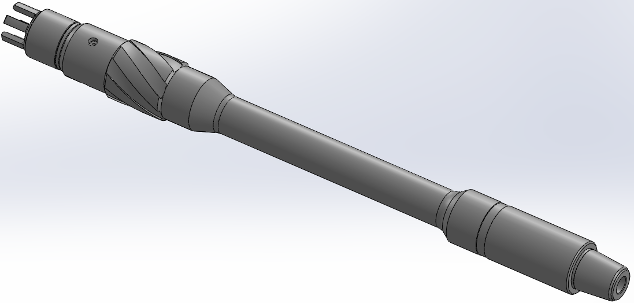
\includegraphics[width=0.5\linewidth]{figure/chapter3/lowwer-sub-mag-tool.png}%
        \label{fig:lowwer_sub_mag_tool}
    }
    \hfill
    % 子图 (b)
    \subfloat[受力件抗扭强度校核]{%
        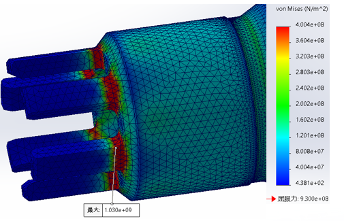
\includegraphics[width=0.4\linewidth]{figure/chapter3/torsion-stress-lowwer-sub-mag-tool.png}%
        \label{fig:torsion_stress_lowwer_sub_mag_tool.png}%
    }
        \caption{受力件抗扭强度有限元分析结果}
    \label{fig:torsion_stress_lowwer_sub_mag_tool}
\end{figure}






\subsubsection{吸附容量计算}

大容量强磁工具的吸附位置主要为四个强磁架处，上端两个强磁架相同，下端两个强磁架相同。
下面为大容量强磁工具吸附容量计算：

7\inch、17lb/ft套管，壁厚为5.87mm，内径为166.06mm。

吸附容量计算 $V_{\max}$ 计算：
\begin{equation}
    V_{\max} = (2 \cdot 5 \cdot s \cdot h + s_1 \cdot h_1 + s_2 \cdot h_2) \times 10^{-6}
\end{equation}
式中，$V_{\max}$---最大吸附容量，L；

$s$---上部强磁沟槽截面面积，$\text{mm}^2$；

$s_1$---上部强磁环空面积，$\text{mm}^2$；

$s_2$---下部强磁环空面积，$\text{mm}^2$；

$h$---强磁环长度，mm；

$h_1$---上部强磁环空长度，mm；

$h_1$---下部强磁环空长度，mm。

大容量强磁吸附容量：
\begin{equation}
	\begin{aligned}
    V_{\max} &= (2 \times 5 \times 603 \times 500 + 7340 \times 1438 + 10343 \times 1420) \times 10^{-6} \\
             &= 28.26< 50\,(\text{L})
	\end{aligned}
\end{equation}

两根工具组合以后容量为 $56.52\,\text{L} > 50\,\text{L}$，满足吸附容量设计要求。


\subsubsection{防退扣部分抗扭计算}
%不清楚这个计算的依据是什么，还要跟曹公再核实一下
大容量强磁工具的防退扣主要薄点为下接头端面键（材料：4145H）。下面为下接头端面键抗扭计算。端面键抗扭危险截面：为端面键截面（键的数量为6）。

防退扣抗扭强度 $\tau$ 计算：
\begin{align}
    \tau &= \frac{T_{\max}}{3 \cdot b \cdot h \cdot d} \times 10^{-6} \\
    T_{\max} &= \frac{3 \cdot [\tau] \cdot b \cdot h \cdot d}{n_1} \times 10^{-6} \\
    [\tau] &= n \cdot \sigma_s = 0.66 \times 827\,\text{MPa} = 545.82\,\text{MPa}
\end{align}
式中，$T_{\max}$---最大防退扣扭矩，$\text{kN}\cdot\text{m}$；

$\sigma_s$---材料屈服应力，$\text{MPa}$；

$d$---危险截面内径，mm；

$b$---端面键宽度，mm；

$h$---端面键高度，mm；

$n$---许用剪应力与许用拉应力系数，根据《机械设计手册》，取 $n = 0.66$；

$[\tau]$---材料许用切应力，$\text{MPa}$；

$n_1$---安全系数，取 $n_1 = 1.5$。

下接头端面键截面防退扣最大扭矩：
\begin{align}
    T_{\max} &= \frac{3 \cdot [\tau] \cdot b \cdot h \cdot d}{n_1} \times 10^{-6} \\
             &= \frac{3 \times 545.82 \times 19 \times 11.75 \times 73.5}{1.5} \times 10^{-6} \\
             &= 17.87\,\text{kN}\cdot\text{m}
\end{align}


综合上述，强磁工具的强度参数见表\ref{tab:mag_tool_force_data}。

\begin{table}[htbp]
    \centering
    \caption{强磁工具受力件数据统计表}
    \label{tab:mag_tool_force_data}
    \renewcommand{\arraystretch}{1.5} % 增加行高，使表格更美观
    \begin{tabularx}{.9\textwidth}{Xc}
        \toprule
        受力类型 & 数据 \\
        \midrule
        NC38 最大拉力 & $3000\,\text{kN}$ \\
        材料屈服强度 $\sigma_s$ & $930\,\text{MPa}$ \\
        螺纹最大剪切力 $F_{\max1}$ & $2950.16\,\text{kN}$ \\
        芯轴最大拉力 $F_{\max2}$ & $1570.81\,\text{kN}$ \\
        NC38 最大扭矩 & $41.30\,\text{kN}\cdot\text{m}$ \\
        材料许用切应力 $[\tau]$ & $620\,\text{MPa}$ \\
        芯轴最大扭力 $T_{\max1}$ & $35.96\,\text{kN}\cdot\text{m}$ \\
        防退扣最大扭矩 $T_{\max2}$ & $17.87\,\text{kN}\cdot\text{m}$ \\
        \bottomrule
    \end{tabularx}
\end{table}

































\subsection{永磁材料选型}

高强磁性体是指那些能够产生强磁场，并在长时间内保持稳定磁性特性的材料。这些材料广泛应用于各种需要强磁力的工业和技术领域。高强磁性体的种类有很多，其中最常见的包括钕铁硼（NdFeB）、钐钴（SmCo）和铝镍钴（AlNiCo）等。在油井清洁打捞作业中，高强磁性体是大容量强磁工具的核心构件。
本项目将以井筒环境为应用基础，调研高强磁性体及高温磁性体的性能，对比筛选出最优产品，建立含磁工具关键结构的数值模拟模型，优化磁性体最大磁性布置规律、给出磁性体安放位置建议，结合磁性体消磁因素分析，给出最优的应用方式，提高工具使用寿命。本章的内容安排如下：

1) 调研钕铁硼、铝镍钴、钐钴等永磁材料在不同温度下的退磁曲线，调研材料退磁的影响因素，对比选择最优永磁材料；

2) 利用ANSYS Maxwell仿真平台建立强磁工具仿真模拟模型，通过改变永磁体充磁方向，探究磁体最大磁性布置规律；

3) 分别建立上部强磁结构和下部强磁结构的仿真模型，探究两种结构对强磁工具最大磁性分布的影响；

4) 通过改变强磁工具上骨架的材料，研究骨架是否为导磁材料对强磁工具最大磁性的影响规律。


永磁材料选择时，应衡量材料工作温度，各温度下的内禀矫顽力（$H_{cj}$）、各温度下的最大磁能积（$BH_{\max}$）等多因素。井筒清洁工具用永磁铁选型的主要依据是工作温度，本项目规定工具的温度设计指标是$150\,^\circ\mathrm{C}$。在满足使用温度的前提下，选择最大磁积能更大的永磁材料，这类次才具有更大的磁性。优先选择内禀矫顽力较大的材料，该类磁材的抗退磁能力和耐温性能更佳，可使得工具在复杂的井筒环境中的具有较好的磁性保持能力，赋予工具良好的稳定性和可靠性。此外还要考虑磁材的经济性和可获得性等辅助因素。

经调研发现，符合井筒清洁工具应用场景的可能材料如表\ref{tab:magnet_params}所示，两种典型磁材：烧结钐钴磁铁（SmCo5）和钕铁硼（N45UH）在不同温度下的退磁曲线如图\ref{fig:demagnetization_SmCo5}、\ref{fig:demagnatization_N45UH}所示。可知，SmCo5在$150\,^\circ\mathrm{C}$-$200\,^\circ\mathrm{C}$的高温环境下，其$H_{cj}$在$-15.8$至$-14.2kOe$之间；N45UH永磁材料在$150\,^\circ\mathrm{C}$-$200\,^\circ\mathrm{C}$的高温环境下，其$H_cj$在$-9.0$至$-6.0kOe$之间。两数据对比可知，虽然在地面环境中N45UH的表观磁性更强，但是当工具下井后，温度升高，其磁性将大大衰减，于是其使用温度一般不超过$120\,^\circ\mathrm{C}$。SmCo5永磁材料因其$H_{cj}$更高，其耐温性和抗退磁能力更好，考虑到本项目中清洁工具$150\,^\circ\mathrm{C}$的设计耐温指标，于是，选用钐钴材料为宜。

\begin{table}[htbp]
    \centering
    \caption{各类永磁材料的性能参数表}
    \label{tab:magnet_params}
    \begin{tabularx}{.9\textwidth}{Xcc}
        \toprule % 顶部粗线
        材料类别 & 居里温度 & 最高工作温度 \\
        \midrule % 中间细线
        铝镍钴 AlNiCo & $750$—$850^\circ\text{C}$ & $450$—$550^\circ\text{C}$ \\
        铁氧体 Ferrite & $> 450^\circ\text{C}$ & $250^\circ\text{C}$ \\
        钐钴 SmCo5 & $700$—$850^\circ\text{C}$ & $250$—$350^\circ\text{C}$ \\
        钕铁硼 H系列 & $340^\circ\text{C}$ & $120^\circ\text{C}$ \\
        \bottomrule % 底部粗线
    \end{tabularx}
\end{table}

\begin{figure}[htbp]
	\centering
	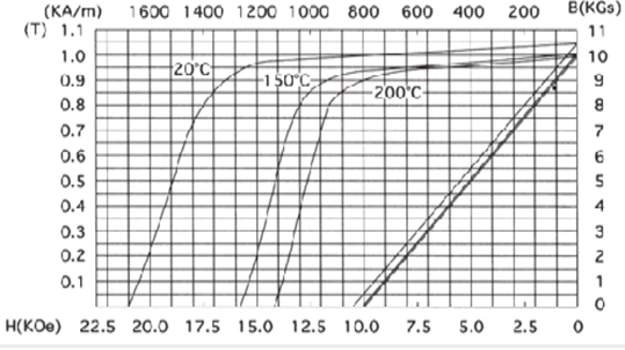
\includegraphics[width=0.7\textwidth]{figure/chapter3/demagnetization-SmCo5.png}
	\caption{喷嘴截面处冲砂液轴向流速对比图}
	\label{fig:demagnetization_SmCo5}
\end{figure}

\begin{figure}[htbp]
	\centering
	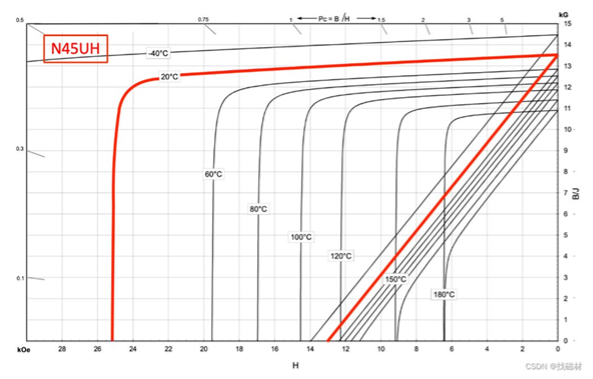
\includegraphics[width=0.7\textwidth]{figure/chapter3/demagnatization-N45UH.png}
	\caption{喷嘴截面处冲砂液轴向流速对比图}
	\label{fig:demagnatization_N45UH}
\end{figure}

\subsection{井筒清洁工具中磁铁布置研究}
在井筒清洁工具中实现磁铁的安装，重点需要考虑的是磁铁部件的安转和夹紧，便于工具的使用和维护，这种结构设计工作甚至需要借鉴设计者在井下工具结构设计方面的经验。在确定工具的基本结构后，需要重点考察磁铁的磁化以其他辅助结构的选材等问题。图为本项目设计的大容量强磁工具，其主要的功能单元包含上部强磁和下部强磁结构（如图2.3(b)、(c)）所示，两部分采用改了不同吸附结构，前者适于吸附小尺度铁质颗粒，后者适于吸附大尺度的铁质颗粒。上部强磁的磁铁放置于带窗的磁铁保护管中，增加与小尺度颗粒的接触面积，每个吸附单元包含两组磁铁，铁质碎屑将吸附于相邻吸附单元之间的空隙中。下部强磁采用开放式结构，磁铁的外圆面暴露于外，增强对大尺寸的铁质碎屑的捕捉能力。给定磁铁材料和吸附结构的情况下，工具的吸附能力主要依赖于磁铁的磁化方向和结构件的材料，下文将对此展开仿真研究。

\begin{figure}[htbp]
    \centering
    % 子图 (a)
    \subfloat[工具磁结构分布]{%
        
\includegraphics[width=0.9\linewidth]{figure/chapter3/magnetic-distribution-on-tool.png}%
        \label{fig:magnet_distribution_on_tool}%
    }
    \vspace{1em}
    % 子图 (b)
    \subfloat[上部强磁局部结构]{%
        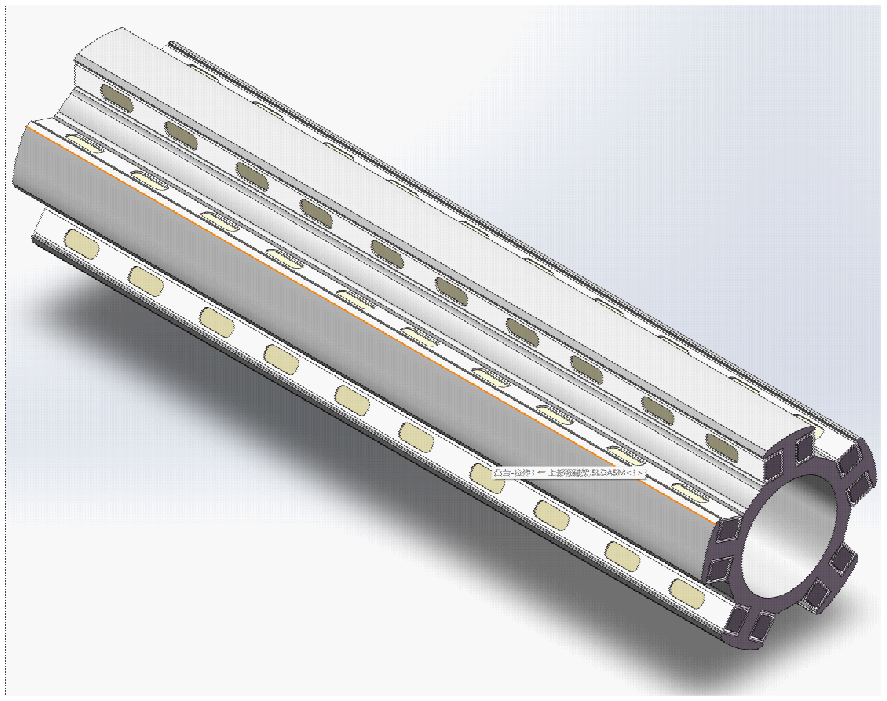
\includegraphics[width=0.4\linewidth]{figure/chapter3/structure-upper-magnetic-sub.png}%
        \label{fig:magnetic_tool_upper_sub}
    }
    \hfill
    % 子图 (c)
    \subfloat[上部强磁局部结构]{%
        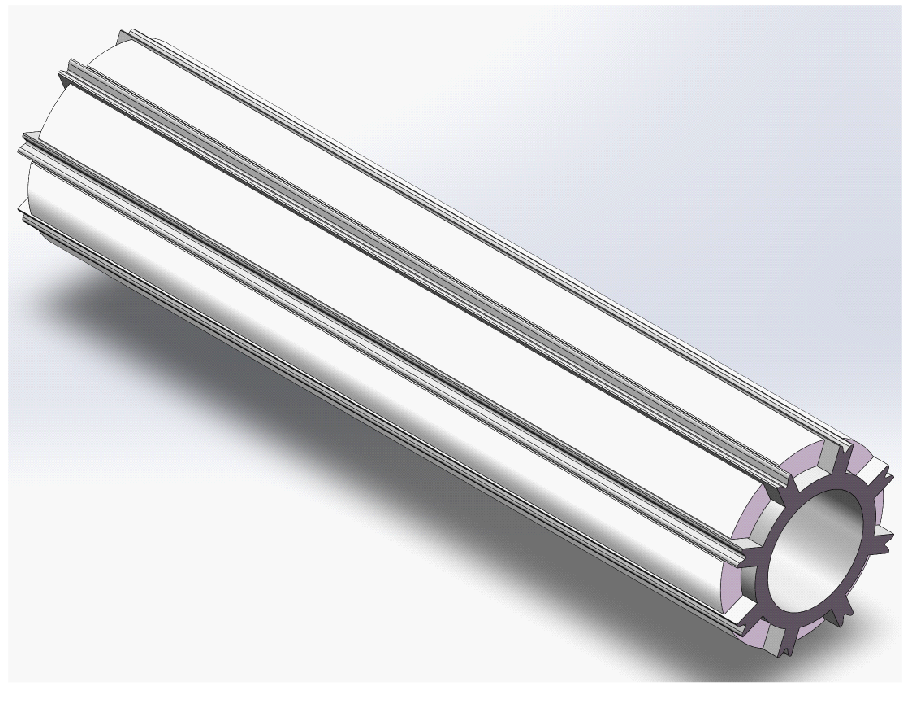
\includegraphics[width=0.4\linewidth]{figure/chapter3/structure-lowwer-magnetic-sub.png}%
        \label{fig:magnetic_tool_lowwer_sub}%
    }
        \caption{大容量强磁工具含磁结构示意图}
    \label{fig:structure_magnetic_tool}
\end{figure}

\subsubsection{强磁工具吸附力理论模型}
在井下环境中，强磁工具上永磁体对井筒内磁性废屑的吸附主要源于永磁体所产生的磁场与磁性材料的相互作用，磁性废屑在永磁体磁场中被磁化产生磁性并与永磁体产生相互作用力。此过程受磁场分布规律、磁场衰减特性、磁性材料磁化程度等多因素影响。
假设磁场均匀分布且磁性废屑与强磁工具上的永磁体直接接触时，其吸附力可利用麦克斯韦应力公式计算：
\begin{equation}
	F=\frac{B^2A}{2\mu_0}
\end{equation}
式中，$B$为永磁体与磁性物质接触表面的磁感应强度，$\mathrm{T}$；$A$为永磁体与磁性物质的接触面积，$\mathrm{m}^2$；$\mu_0$为真空磁导率常数，$\mu_0=4\pi×10^(-7) \mathrm{H/m}$。

当磁性铁屑与磁铁存在一定距离$d$时，吸附力需考虑磁场梯度的影响，这时永磁体对磁性碎屑的吸引力可表示为
\begin{equation}
	F=\frac{3\mu_0 m_1m_2}{4\pi d^4}
\end{equation}
式中，$m_1$ 、$m_2$分别为永磁体与磁性物质的磁矩，单位$\mathrm{A}\cdot \mathrm{m}^2$。

永磁体磁矩$m_1$的计算式为
\begin{equation}
	m_1=\frac{B_rV_1}{\mu_0}
\end{equation}
式中，$B_r$为永磁体剩磁，$\mathrm{T}$；$V_1$为永磁体体积，$\mathrm{m}^3$。

铁屑的磁矩$m_2$与所处的外磁感应场强度$B$有关，计算式为
	\begin{equation}
		m_2 = \frac{\gamma B V_2}{\mu_0}
	\end{equation}
式中，$\gamma$为磁性物质的磁化率，通常铁磁材料的$\gamma≫1$，量纲为1；$V_2$为磁性物质体积，$\mathrm{m}^3$。

综合以上两式，铁屑受到的磁力为
\begin{equation}
	F=\frac{3V_1V_2BB_r\gamma}{4\pi d^4}
\end{equation}

综上所述，在井下强磁工具吸附磁性废屑过程中，当永磁体体积参数确定时，体积越大、距离工具越近，周围磁场强度更高的磁性碎屑所受吸附力越大。在井下碎屑参数未知时，可选择高温度下剩磁高、体积大的磁体，以及保证工具外侧磁场强度大来产生足够大的吸附力。但采用解析方法精确计算碎屑受到的磁力难度较大：一方面，单个永磁体要受到其他永磁体及工具复杂结构的影响，永磁体的剩磁$B_r$难以确定；另一方面，磁性碎屑相互有之间会产生磁场的干扰，磁性碎屑堆积形成的碎屑床形状不规则，碎屑和磁铁之间的距离不能事先预测。于是，下文采用有限元的方法对工具空载（没有磁性碎屑存在）的条件下对工具周围磁场进行研究，作为一个表征工具碎屑吸附性能的间接指标，进而探索对工具性能产生影响的结构参数的影响。

\subsubsection{上部结构磁铁仿真模拟}

上部强磁结构为一三维结构，工具中的磁场应是一个复杂的三维空间磁场。但除端部外，其有效的功能单元是可看成是沿轴向均布的，于是，可考虑采用采用二维模型对所研究的问题进行简化。在ANSYS Maxwell软件中建立如图2.5所示的Maxwell 2D静磁场。永磁体材料选择井筒工作温度为$180\,^\circ \mathrm{C}$下的钐钴（SmCo5）材料，骨架材料选择4145牌号的钢材，永磁体保护套材料为304钢，各材料的属性列举于表\ref{tab:smco5_params}—表\ref{tab:304_properties_180c}中。


\begin{figure}[htbp]
	\centering
	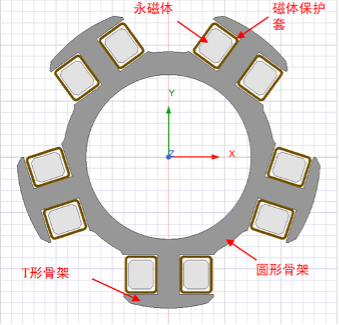
\includegraphics[width=0.5\textwidth]{figure/chapter3/magnet-configuration-upper-sub.png}
	\caption{强磁工具上部结构模型}
	\label{fig:magnet_configuration_upper_sub}
\end{figure}



\begin{table}[htbp]
    \centering
    \caption{$180\,^\circ\mathrm{C}$ SmCo5磁材性能参数表}
    \label{tab:smco5_params}
    \begin{tabularx}{.9\textwidth}{Xccc}
        \toprule
        参数 & 符号 & 数值 & 单位 \\
        \midrule
        相对磁导率 & $\mu$ & 1.09 & - \\
        剩磁 & $B_r$ & 0.8 & T \\
        电导率 & $\sigma$ & 1500000 & Siemens/s \\
        \midrule
        矫顽力 & $H_{cj}$ & $-15$ & kOe \\
        \bottomrule
    \end{tabularx}
\end{table}

\begin{table}[htbp]
    \centering
    \caption{$180\,^\circ\mathrm{C}$ 4145钢材性能参数表}
    \label{tab:steel_params}
    \begin{tabularx}{.9\textwidth}{Xccc}
        \toprule
        参数 & 符号 & 数值 & 单位 \\
        \midrule
        相对磁导率 & $\mu$ & 200 & --- \\
        电导率 & $\sigma$ & 4250000 & Siemens/s \\
        杨氏模量 & $E$ & 195 & GPa \\
        泊松比 & $\nu$ & 0.3 & --- \\
        \bottomrule
    \end{tabularx}
\end{table}

\begin{table}[htbp]
  \centering
  \caption{$180\,^\circ \mathrm{C}$下304不锈钢性能参数表}
  \label{tab:304_properties_180c}
  \begin{tabularx}{.9\textwidth}{Xccc}
    \toprule
    参数 & 符号 & 数值 & 单位 \\
    \midrule
    相对磁导率 & $\mu$ & 1 & --- \\
    电导率 & $\sigma$ & 1200000 & Siemens/s \\
    杨氏模量 & $E$ & 185 & GPa \\
    泊松比 & $v$ & 0.3 & --- \\
    \bottomrule
  \end{tabularx}
\end{table}


对于图\ref{fig:magnet_configuration_upper_sub}给定的磁铁、保护套和骨架结构，磁铁有图\ref{fig:two_magnetization_upper_sub}所示两种磁化方向，下文分别称为径向磁化和周向磁化。求解域设置为边长300mm的矩形，在其四条边上设置气球边界条件，网格划分，磁体与其保护套上最大网格尺寸0.5mm，上部结构骨架上最大网格尺寸2mm，求解步设置计算至收敛。在计算域中设置一个边长为200mm的矩形观测区域以观测仿真结果，以进行仿真结果后处理。

\begin{figure}[htbp]
    \centering
    % 子图 (a)
    \subfloat[径向磁化]{%
        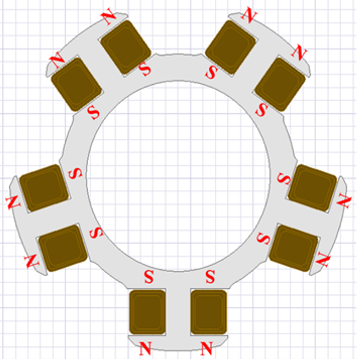
\includegraphics[width=0.35\linewidth]{figure/chapter3/radial-magnetization-in-upper-sub.png}%
        \label{fig:radial_magnetization_in_upper_sub}
    }
    %\hfill
    % 子图 (b)
    \subfloat[周向磁化]{%
        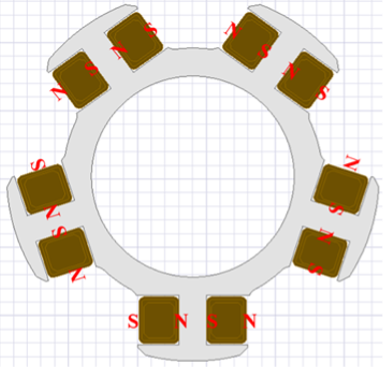
\includegraphics[width=0.35\linewidth]{figure/chapter3/circumferencial-magnetization-in-upper-sub.png}%
        \label{fig:circumferencial_magnetization_in_upper_sub}%
    }
        \caption{上部强磁两种磁化方向示意图}
    \label{fig:two_magnetization_upper_sub}
\end{figure}

\begin{figure}[htbp]
    \centering
    % 子图 (a)
    \subfloat[边界条件设置]{%
        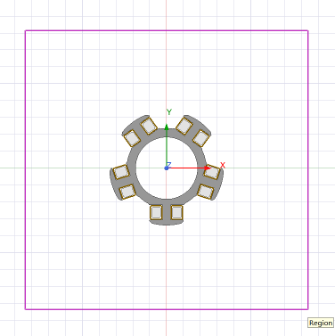
\includegraphics[width=0.35\linewidth]{figure/chapter3/boundary-condition-upper-sub.png}%
        \label{fig:boundary_condition_upper_sub}
    }
    \hfill
    % 子图 (b)
    \subfloat[计算域网格划分]{%
        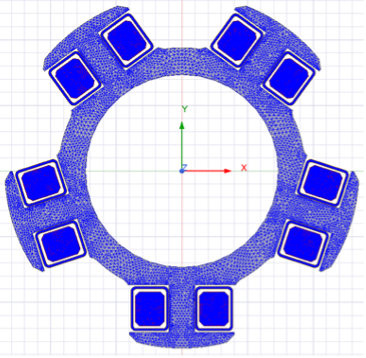
\includegraphics[width=0.35\linewidth]{figure/chapter3/mesh-upper-sub.png}%
        \label{fig:mesh_upper_sub}%
    }
        \caption{上部强磁磁场分析设置}
    \label{fig:computation_setup_upper_sub}
\end{figure}

(1) 径向充磁仿真结果及讨论

由于强磁工具在其使用工况下是通过其外侧磁场的作用吸附碎屑，因此在仿真结果中以强磁工具表面磁场强度为分析对象。

由观测面上的磁感应强度云图可知，最大磁感应强度$B=7.9T$，出现在永磁体安装T型骨架沟槽的顶部和底部；各永磁体表面的$B$值在$0.5$—$1.5T$范围内，但是受304不锈钢制的永磁体保护套影响，保护套外侧$B$值在$0.2$—$0.7T$范围内，T型骨架表面的$B$值在$0.6$—$1.4T$范围内，而圆形骨架的B值较低大部分在$0.5T$以下，从结果来看，304不锈钢制的永磁体保护套会使工具外侧的磁场强度变低。

\begin{figure}[htbp]
    \centering
    % 子图 (a)
    \subfloat[磁场矢量分布]{%
        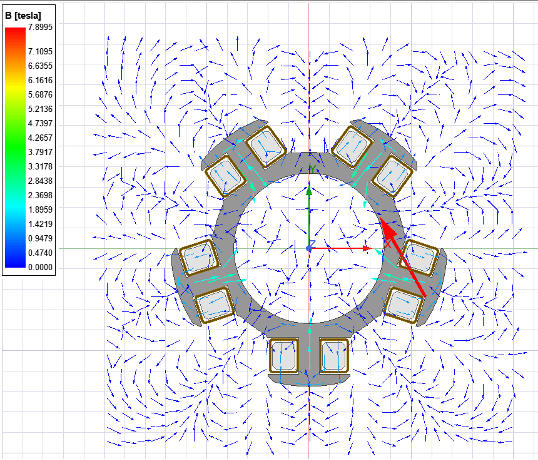
\includegraphics[width=0.45\linewidth]{figure/chapter3/magnetic-vector-distribution-upper-sub.png}%
        \label{fig:magnetic_vector_distribution_upper_sub}
    }
    %\hfill
    % 子图 (b)
    \subfloat[磁感应强度分布]{%
        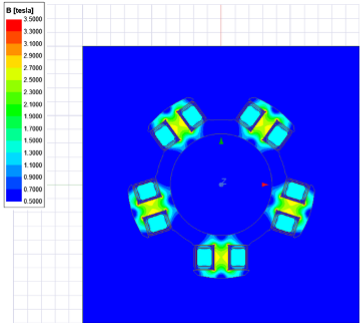
\includegraphics[width=0.45\linewidth]{figure/chapter3/contour-magnetic-field-upper-sub.png}%
        \label{fig:contour_magnetic_field_upper_sub}%
    }
        \caption{磁铁径向磁化时上部强磁组件磁场计算结果}
    \label{fig:field_result_in_upper_sub_radial_magnetization}
\end{figure}

(2) 周向充磁仿真结果及讨论

观察磁感应强度云图可知，观测面上最大磁感应强度$B=2.9T$，出现在T型骨架沟槽最顶部，永磁体内的$B$值在$0.6$—$1.3T$范围内，保护套上$B$值在$0.5$—$0.9T$范围内，T型骨架沟槽中的B值在$0.4$-$1.3T$范围内，而圆形骨架的$B$值在$0.3$—$0.8T$范围内。

\begin{figure}[htbp]
    \centering
    % 子图 (a)
    \subfloat[磁场矢量分布]{%
        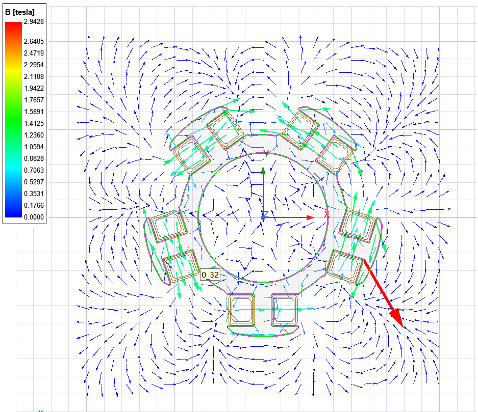
\includegraphics[width=0.45\linewidth]{figure/chapter3/magnetic-vector-distribution-upper-sub-circum-magnatization.png}%
        \label{fig:magnetic_vector_distribution_upper_sub_circum_magnatization.png}
    }
    \hfill
    % 子图 (b)
    \subfloat[磁感应强度分布]{%
        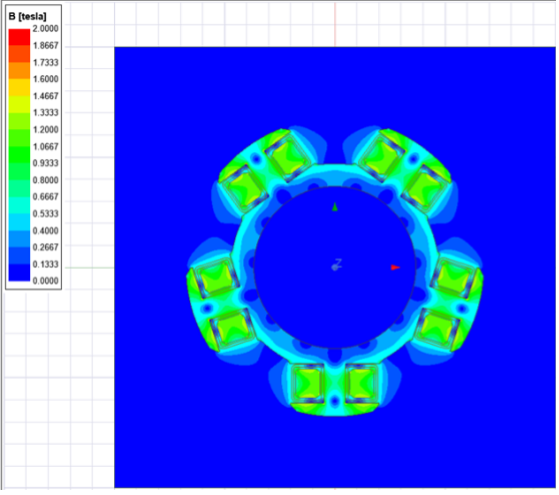
\includegraphics[width=0.45\linewidth]{figure/chapter3/contour-magnetic-field-upper-sub-circum-magnatization.png}%
        \label{fig:contour_magnetic_field_upper_sub_circum_magnatization}%
    }
        \caption{磁铁周向磁化时上部强磁组件磁场计算结果}
    \label{fig:field_result_in_upper_sub_radial_magnetization}
\end{figure}


上部结构中的两种充磁方式中，周向充磁磁场分布更加均匀，但最大磁感应强度值远小于径向充磁磁场，分析得出上部结构类型导致T型骨架和圆形骨架上的磁场分布存在差异，T型骨架上的场强大于圆形骨架上场强，不锈钢制的磁铁保护套会降低永磁体表面的磁场强度。分析两种充磁方式下各部表面磁感应强度表可知，周向充磁与径向充磁相比，永磁体及其保护套、T形骨架表面上的磁场强度差异较小，但圆形骨架表面磁场强度大于周向充磁时的磁场强度，周向充磁时磁场分布更加均匀，因此，对于上部结构宜选用周向充磁方式。

%这里差一个表2.5

\subsubsection{下部结构仿真模拟}

强磁工具下部结构为一对称结构，永磁体均匀排列在其骨架上，为方便仿真计算，将下部结构简化为二维模型求解，在ANSYS Maxwell软件中建立如图\ref{fig:magnet_configuration_lowwer_sub}所示的强磁工具下部结构仿真模型。永磁体材料选择井筒工作温度为180℃下的钐钴SmCo5材料，骨架材料选择4145牌号的钢材，各材料的属性见表\ref{tab:smco5_params}—表\ref{tab:304_properties_180c}。

\begin{figure}[htbp]
	\centering
	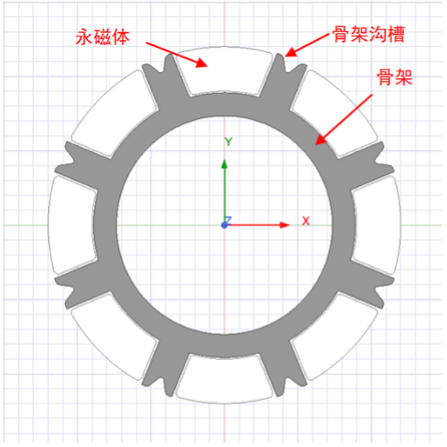
\includegraphics[width=0.5\textwidth]{figure/chapter3/magnet-configuration-lowwer-sub.png}
	\caption{强磁工具上部结构模型}
	\label{fig:magnet_configuration_lowwer_sub}
\end{figure}

对于强磁工具下部结构，磁铁有图2.6所示的同一径向磁化、交叉径向磁化、周向磁化三种磁化方向，其他仿真参数与上部结构仿真模型相同，如图\ref{fig:computation_setup_lowwer_sub}所示，对观测面上的仿真结果进行分析。三种磁化方式对应的磁场分布如图\ref{fig:field_result_in_lowwer_sub_3_magnetization}所示。


\begin{figure}[htbp]
    \centering
    % 子图 (a)
    \subfloat[同一径向磁化]{%
        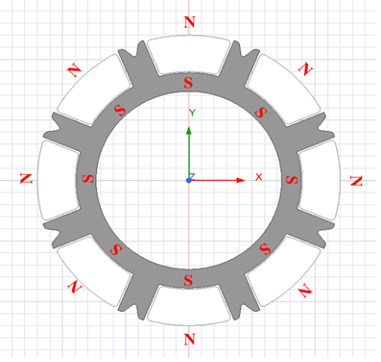
\includegraphics[width=0.4\linewidth]{figure/chapter3/lowwer-sub-magnetization-radial.png}%
        \label{fig:lowwe_sub_magnetization_radial}%
    }
    \vspace{1em}
    % 子图 (b)
    \subfloat[交叉径向磁化]{%
        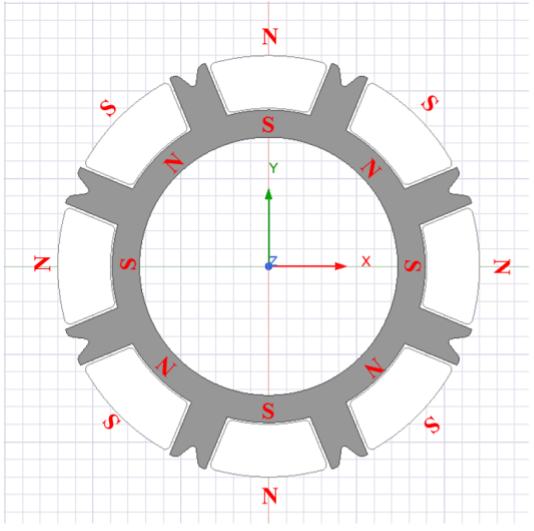
\includegraphics[width=0.4\linewidth]{figure/chapter3/lowwer-sub-cross-magnetization.png}%
        \label{fig:lowwer_sub_cross_magnetization}
    }
    \hfill
    % 子图 (c)
    \subfloat[周向磁化]{%
        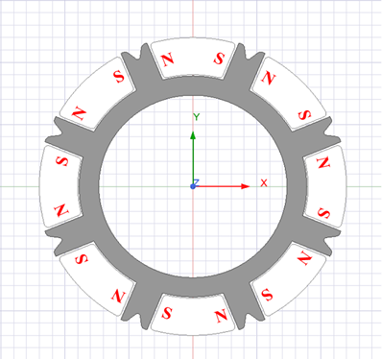
\includegraphics[width=0.4\linewidth]{figure/chapter3/lowwer-sub-circumferential-magnetization.png}%
        \label{fig:lowwer_sub_circumferential_magnetization}%
    }
        \caption{下部强磁磁化方向示意图}
    \label{fig:lowwer_sub_magnetization_3ways}
\end{figure}


\begin{figure}[htbp]
    \centering
    % 子图 (a)
    \subfloat[边界条件设置]{%
        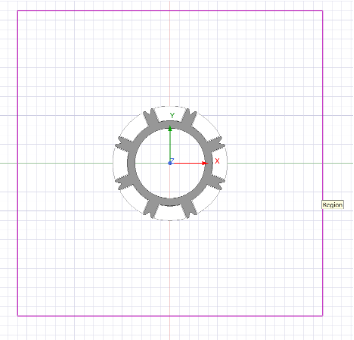
\includegraphics[width=0.4\linewidth]{figure/chapter3/boundary-condition-lowwer-sub.png}%
        \label{fig:boundary_condition_lowwer_sub}
    }
    %\hfill
    % 子图 (b)
    \subfloat[计算域网格划分]{%
        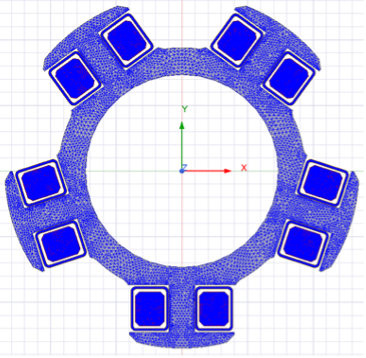
\includegraphics[width=0.4\linewidth]{figure/chapter3/mesh-upper-sub.png}%
        \label{fig:mesh_lowwer_sub}%
    }
        \caption{下部强磁磁场分析设置}
    \label{fig:computation_setup_lowwer_sub}
\end{figure}



\begin{figure}[htbp]
    \centering
    % 子图 (a)
    \subfloat[磁场矢量分布]{%
        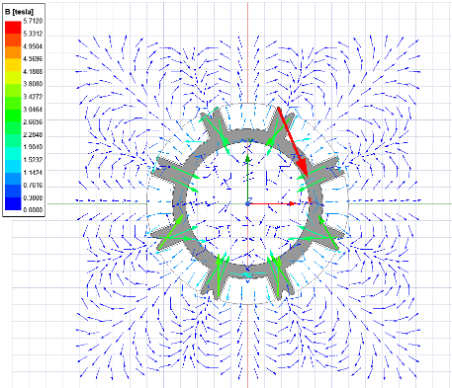
\includegraphics[width=0.45\linewidth]{figure/chapter3/magnetic-vector-distribution-lowwer-sub-radial.png}%
        \label{fig:magnetic_vector_distribution_lowwer_sub_radial}
    }
    %\hfill
    % 子图 (b)
    \subfloat[磁感应强度分布]{%
        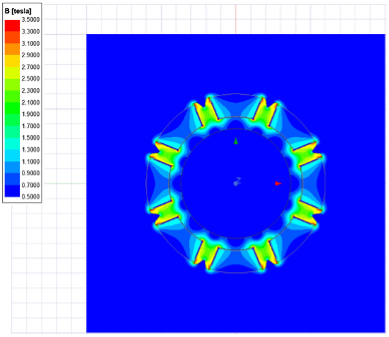
\includegraphics[width=0.45\linewidth]{figure/chapter3/contour-magnetic-field-lowwer-sub-radial.png}%
        \label{fig:contour_magnetic_field_lowwer_sub_radial}%
    }
    \vspace{1em}
     % 子图 (c)
    \subfloat[磁场矢量分布]{%
        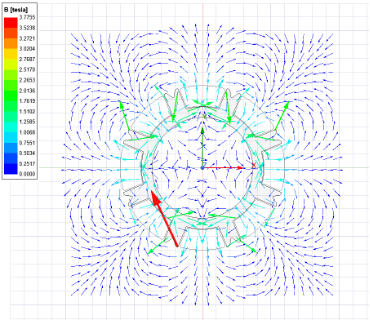
\includegraphics[width=0.45\linewidth]{figure/chapter3/magnetic-vector-distribution-lowwer-sub-cross.png}%
        \label{fig:magnetic_vector_distribution_lowwer_sub_cross}
    }
   % \hfill
    % 子图 (d)
    \subfloat[磁感应强度分布]{%
        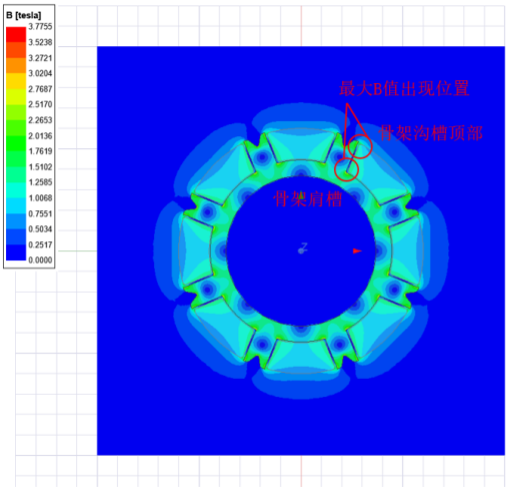
\includegraphics[width=0.45\linewidth]{figure/chapter3/contour-magnetic-field-lowwer-sub-cross.png}%
        \label{fig:contour_magnetic_field_lowwer_sub_cross}%
    }
    \vspace{1em}
     % 子图 (e)
    \subfloat[磁场矢量分布]{%
        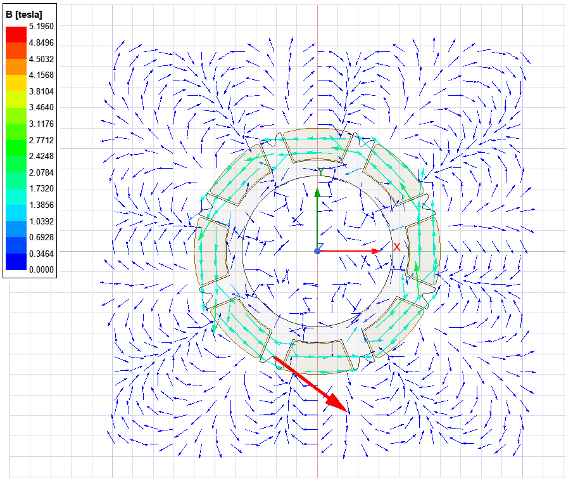
\includegraphics[width=0.45\linewidth]{figure/chapter3/magnetic-vector-distribution-lowwer-sub-circumferential.png}%
        \label{fig:magnetic_vector_distribution_upper_sub_circumferential}
    }
   % \hfill
    % 子图 (f)
    \subfloat[磁感应强度分布]{%
        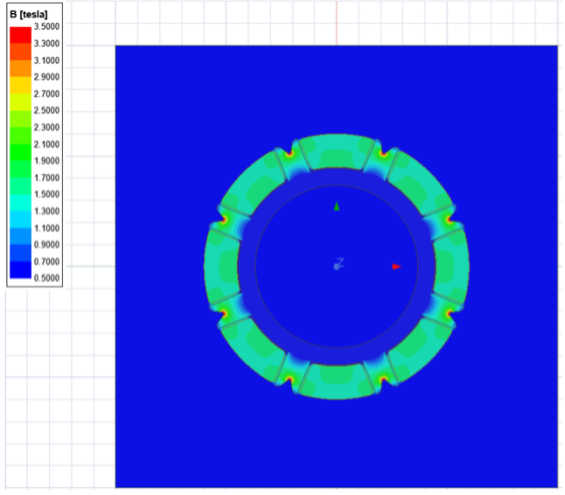
\includegraphics[width=0.45\linewidth]{figure/chapter3/contour-magnetic-field-lowwer-sub-circumferential.png}%
        \label{fig:contour_magnetic_field_upper_sub_circumferential}%
    }


        \caption{磁铁采用不同磁化方式时下部强磁组件磁场计算结果}
    \label{fig:field_result_in_lowwer_sub_3_magnetization}
\end{figure}




(1) 同一径向充磁仿真结果及讨论

由观测面上的磁感应强度云图可知，磁感应强度成对称分布，最大磁感应强度B=5.7 T，出现在永磁体安装骨架的肩槽和骨架沟槽顶部，各永磁体表面的B值在0.5—1.5T范围内，骨架沟槽表面的B值在骨架最凹处最小沿沟槽向两侧增大其数值在0.5—3.5T范围内。

(2) 交叉径向充磁仿真结果及讨论

由观测面上的磁感应强度云图可知，磁感应强度称对称分布，最大磁感应强度B=3.8 T，出现在永磁体安装骨架的肩槽和骨架沟槽顶部，各永磁体表面的B值在0.7—1.5T范围内，骨架沟槽表面的B值在1.2—3.5T范围内。

(3) 周向充磁仿真结果及讨论

由观测面上的磁感应强度云图可知，云图上最大磁感应强度B=5.2T出现在骨架沟槽最凹点处，各永磁体上的B值在1.3—1.7T范围内，骨架沟槽表面最凹点B值最大沿沟槽向两侧减小，其数值在0.7-3.5T范围内。


由基于充磁方式的下部强磁工具仿真结果总结于表\ref{tab:magnetic_intensity}，由此可得出，永磁体表面的磁感应强度周向充磁时略强于径向充磁时，分析骨架沟槽的表面的磁感应强度可知，同一径向充磁和周向充磁时，骨架沟槽上的磁感应强度梯度大，交叉径向充磁时骨架沟槽表面的磁感应强度分布更均匀。同一径向充磁和周向充磁时，磁感线会富集到骨架沟槽内造成骨架沟槽内的磁感应强度大，而工具外侧的磁感应强度小。因此，下部结构宜选择交叉径向充磁方式。

\begin{table}[htbp]
    \centering
    \caption{下部结构各部表面磁感应强度数据}
    \label{tab:magnetic_intensity}
    \begin{tabularx}{.9\textwidth}{Xccc} % 第一列左对齐(l)，后三列居中(c)
        \toprule
        % 第一行：左侧标题 + 右侧跨3列的标题
        强磁工具结构 & \multicolumn{3}{c}{下部结构} \\
        \midrule
        % 第二行：具体的充磁类型分类
        充磁类型 & 同向径向充磁 & 交叉径向充磁 & 周向充磁 \\
        \midrule
        % 第三行：数据
        永磁体表面 & 0.5---1.5T & 0.7---1.5T & 1.3---1.7T \\
        % 第四行：数据
        骨架沟槽表面 & 0.5---3.5T & 1.2---3.5T & 0.7---3.5T \\
        \bottomrule
    \end{tabularx}
\end{table}

\subsection{两种结构对强磁工具最大磁性分布的影响}

本节依据上节两种强磁工具结构的仿真结果，通过数据对比分析两种结构对强磁工具磁性分布的影响。强磁工具各部表面磁感应强度数值由磁场探针测得，测量数据见表\ref{tab:strong_magnet_data}。



\begin{table}[htbp]
    \centering
    \caption{强磁工具各部表面磁感应强度数据表}
    \label{tab:strong_magnet_data}
    % 设置列格式：第一列左对齐，其余居中。p{}用于控制长文本换行
    \begin{tabular}{lcccccc}
        \toprule
        % 第一行表头：上部结构(跨2列)，下部结构(跨3列)
        强磁工具结构 & \multicolumn{2}{c}{上部结构} & \multicolumn{4}{c}{下部结构} \\
        \cmidrule(r){2-3} \cmidrule(l){4-7} % 子表头下方的横线，r/l控制留白
        % 第二行表头：具体的充磁类型
        充磁类型 & 径向充磁 & 周向充磁 & \shortstack{同向径向\\充磁} & \shortstack{交叉径向\\充磁} & \multicolumn{2}{c}{周向充磁} \\
        \midrule
        % 数据行 1
        永磁体表面 & 0.5---1.5T & 0.6---1.3T & 0.5---1.5T & 0.7---1.5T & \multicolumn{2}{c}{1.3---1.7T} \\
        % 数据行 2 (包含合并行 "骨架沟槽表面")
        T型骨架表面 & 0.6---1.4T & 0.4---1.3T & \multirow{2}{*}{\shortstack{骨架沟槽\\表面}} & 0.5---3.5T & 1.2---3.5T & 0.7---3.5T \\
        % 数据行 3
        圆形骨架表面 & 0---0.3T & 0.3---0.8T & & - & - & - \\
        % 数据行 4
        保护套表面 & 0.2---0.7T & 0.5---0.9T & - & - & - & - \\
        \bottomrule
    \end{tabular}
\end{table}

由强磁工具的上、下部结构在不同充磁方向下的各部位表面磁场数据得出，对于上部结构，由于其结构影响T型骨架和圆形骨架上的磁场分布差异较大，T型骨架上场强大于圆形骨架上的场强，且不锈钢保护套会造成永磁体表面磁场衰减，改变永磁体充磁方向后磁场分布仍呈现此情况；对于下部结构，不同的充磁方向对其表面磁场分布影响很大，永磁体采用交叉径向充磁时，工具永磁体和骨架的表面磁场分布均匀。综上所述，采用交叉径向充磁的下部强磁工具结构的表面磁场分布均匀，易于强磁工具在井筒内的大面积吸附工作。


\subsection{强磁工具骨架材料对最大磁性分布的影响}

利用2.2.4小节中的下部工具结构仿真模型数据，保持其他仿真参数不变，在永磁体交叉径向充磁的工况下，将强磁工具骨架材料设置为不导磁的铝材，铝材参数如表\ref{tab:aluminum_params}所示，观察仿真结果中工具表面磁场分布。下部结构交叉径向充磁时，铝制骨架与4145钢制骨架模型的仿真结果进行对比分析图\ref{fig:mag_field_frame_material}。

\begin{table}[htbp]
    \centering
    \caption{180$^\circ$C下铝材参数表}
    \label{tab:aluminum_params}
    \begin{tabularx}{.9\textwidth}{Xccc}
        \toprule
        参数 & 符号 & 数值 & 单位 \\
        \midrule
        相对磁导率 & $\mu$ & 1.00021 & --- \\
        电导率 & $\sigma$ & 38000000 & Siemens/s \\
        杨氏模量 & $E$ & 69 & GPa \\
        泊松比 & $\nu$ & 0.31 & --- \\
        \bottomrule
    \end{tabularx}
\end{table}

\begin{figure}[htbp]
    \centering
    % 子图 (a)
    \subfloat[4145钢制骨架]{%
        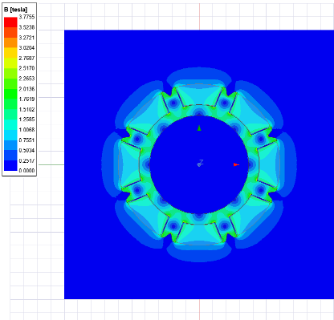
\includegraphics[width=0.4\linewidth]{figure/chapter3/mag-field-distribution-4145-steel-frame.png}%
        \label{fig:mag_field_distribution_4145_steel_frame}
    }
    \hfill
    % 子图 (b)
    \subfloat[铝制骨架]{%
        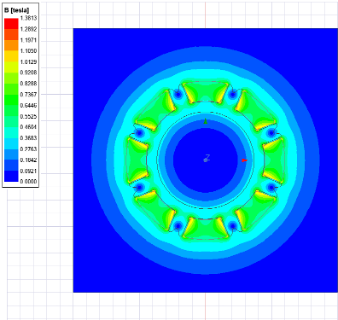
\includegraphics[width=0.4\linewidth]{figure/chapter3/mag-field-distribution-aliminium-frame.png}%
        \label{fig:mag_field_distribution_aliminium_frame}%
    }
        \caption{骨架材料对磁场分布的影响}
    \label{fig:mag_field_frame_material}
\end{figure}

表\ref{tab:aluminum_vs_4145_steel}为下部强磁工具结构交叉径向充磁模型的4145钢制骨架和铝制骨架仿真结果对比。由铝制骨架仿真结果得出，铝制骨架导致工具磁场中的最大场强降低，铝制骨架沟槽内的磁场强度低于4145钢制骨架沟槽内的磁场强度，分析得出骨架材料宜选用导磁效果好，可磁化程度高的金属合金材料，以起到聚集磁感线增大磁通的效果。


\begin{table}[htbp]
    \centering
    \caption{铝制骨架与4145钢制骨架工具表面磁场数据对比}
    \label{tab:aluminum_vs_4145_steel}
    \begin{tabularx}{.9\textwidth}{Xcc}
        \toprule
        强磁工具结构 & \multicolumn{2}{c}{下部结构} \\
        \cmidrule(r){2-3}
        充磁类型 & \multicolumn{2}{c}{周向充磁} \\
        \cmidrule(r){2-3}
        骨架材料 & 4145 钢制 & 铝制 \\
        \midrule
        永磁体表面 & 0.7---1.5T & 0.3---0.7T \\
        骨架沟槽表面 & 1.2---3.5T & 0.2---0.4T \\
        \bottomrule
    \end{tabularx}
\end{table}

\subsection{永磁材料的退磁影响因素}

永磁体的退磁是影响其长期稳定性和应用可靠性的关键问题，退磁由多种因素引起。

（1）居里温度

居里温度是磁性材料在铁磁性物质/亚铁磁性物质和顺磁性物质之间改变的温度。温度超过居里温度，磁体内部分子剧烈运动并出现不可逆的退磁情况，磁体退磁后可再次被充磁，但磁力会大幅下降，仅能达到原来的50\%左右。

（2）工作温度

在工作温度内温度升高磁力会下降，但是不超过居里温度的情况下，降温后磁力大部分会恢复，工作温度范围内发生可逆性退磁。

（3）外部磁场

外部强反向磁场（如电机电枢反应、短路电流）可能超过磁体的矫顽力，导致磁体部分或完全退磁。

（4）时间因素

随着时间的延长磁体内部微观结构（如晶粒边界、杂质相）随时间缓慢变化，导致剩磁轻微衰减，通常每年衰减小于1\%。

（5）机械冲击

机械应力可能破坏磁体内部的磁畴排列，尤其是脆性材料（如钕铁硼），避免直接敲击或跌落磁体。在复杂振动环境中增加缓冲结构（如橡胶垫）。

（6）化学侵蚀

在高温、高湿的酸碱环境下，钕铁硼磁体因含钕、铁易氧化（生锈），导致磁通量下降甚至断裂。在不稳定的化学环境下对磁体进行表面涂层（如镍、锌、环氧树脂、电镀层）或密封封装以隔绝环境影响。

具体到井筒清洁工具设计，具体到井筒清洁工具的设计，选择的钐钴磁铁耐温达到了450—550$^\circ$C，磁材的居里温度为750—850$^\circ$C，远超工具的设计温度指标150$^\circ$C，可保证磁铁不会因温度因素而退磁，在重复使用过程中，可保证磁材都是可逆退磁。井筒中不存在可能使磁铁退磁强外部磁场，磁铁在工作过程中的退磁效应可忽略。在工具长时间存储时，可考虑采用铁磁质材料制作的磁路附件使得磁材的磁路闭合，减少磁材磁性的衰减。在机械结构设计上，磁铁外设计了不锈钢制作的保护套，以减少清洁工具在运输和使用过程中产生的冲击直接作用于磁铁本身，减少机械冲击。在磁铁在制造过程中表面采用镀镍工艺，易蚀性磁材本体和腐蚀性的环境隔离开来，磁铁在安装过程中设置了安装规范，减少磁材表面划伤，严禁损伤磁材下井。

\subsubsection{强磁工具操作方式}

（1）使用方法

根据井眼尺寸选择合适的强磁吸附工具。强磁工具通过钻柱送入井底完成吸附打捞作业，如情况允许也可以通过钢丝绳送入井底。

（2）操作方法

该工具可以与ZKG模块化多合一套管清洁工具一同使用（推荐），也可以在刮完井之后使用。将强磁吸附工具放在预先放好木板的转盘上（防止强磁吸附工具与转盘发生吸附），并接于钻柱底部，然后提起，取掉木板，准备下井。将DQC大容量强磁吸附工具下到井下离通井位置3-5m处，开泵循环。将DQC大容量强磁吸附工具在该位置上下活动。保持循环，平稳地上提钻柱。起钻时要求平稳、低速、严禁剧烈震动与撞击，以保护强磁部件。

\subsubsection{强磁工具维护与保养}

DQC大容量强磁吸附工具每次使用后，应放在没有铁屑和杂物区域内的木板或橡胶板上，清除干净吸附在强磁工具表面的金属颗粒和铁屑粉末，然后用清水清洗各零件。工具在井下工作多次后，或在恶劣条件下工作后，应进行维护修理，将其全部拆开、检查、重新装配。



本节首先调研了钕铁硼、铝镍钴、钐钴等永磁材料的工作参数及退磁曲线，确定了钐钴材料为井下强磁工具上的永磁体材料并分析了永磁体退磁影响因素；其次，利用ANSYS Maxwell软件构建了上部强磁结构和下部强磁结构的仿真模型，通过改变工具中永磁体充磁方式及骨架材料，探究其最大磁性分布规律；在基于充磁方向的磁体布置研究中得出，上部结构宜采用径向充磁方式，下部结构宜采用周向充磁方式来达到磁场分布均匀且保证最大磁性的目的；在基于骨架材料对最大磁性分布的影响研究中得出，骨架材料为导磁效果好的金属材料时，能聚集磁感线增大磁通，起到增加工具磁性的作用。


































































\chapter{多功能过滤工具设计}
	% !TeX root = ../../main.tex
\section{工具总体结构设计}

多功能过滤工具\footnote{下文简称为“过滤工具”}是井筒高效清洁配套工具中的关键工具之一，由钻杆送入井下，在起钻过程中对井下钻井液进行过滤，分离并收集井底碎屑。其过滤功能独立于其他井下作业，不会影响正常下钻及循环。停泵上提过程中，该工具处于工作状态，扶正套筒移动并打开工具内部通道口，钻井液经工具内部的过滤外筒过滤后下行。

多功能过滤工具采用扶正套筒开关设计：下入时，扶正套筒关闭工具内部通道口，不影响工具串正常下钻及作业；上提时，扶正套筒打开工具内部通道口，过滤工具开始工作。

多功能过滤工具设置有观察孔及清理盖板：观察孔便于检查碎屑的收集量；清理盖板在工具作业完成后即可拆卸，以清理储存的碎屑，无需拆卸工具本体。

多功能过滤工具的结构如图~\ref{fig:filter_tool_structure}所示，主要由提升短节、上扶正套筒、扶正块、滤进接头、过滤套筒、过滤外筒、过滤内筒、清理盖板、滤出接头、下扶正套筒和下接头组成。其中，过滤套筒、过滤外筒和过滤内筒可替换为加长版，以增大过滤容量。

其工作原理为：工具下井后，扶正套筒受力上行，关闭工具内部通道口，此时过滤工具不工作，工具串可进行正常作业；当工具串上提时，扶正套筒受力下行，打开工具内部通道口，过滤工具开始工作。带有碎屑的钻井液进入工具内部，由过滤外筒完成过滤，经过滤内筒循环回井内。

\begin{figure}[htbp]
  \centering % 图片居中
  \includegraphics[width=1.0\textwidth]{figure/chapter3/guolvqi.png} % 图片路径
  \caption{多功能过滤工具结构示意图} % 图标题
  \label{fig:filter_tool_structure} % 标签，用于文中引用
\end{figure}

过滤工具的主要技术参数见表~\ref{tab:filter_tool_params}。

\begin{table}[htbp]
    \centering
    \caption{多功能过滤工具技术参数表}
    \label{tab:filter_tool_params}
    \footnotesize % 共 11 列，缩小字号以适应宽表格
    \setlength{\tabcolsep}{3pt} % 减小列间距，避免超出正文版心
    \renewcommand{\arraystretch}{1.3} % 增加行高
    
    \begin{tabularx}{\textwidth}{Xcccccccccc}
        \toprule
        型号 & 
        \begin{tabular}[c]{@{}c@{}}适用\\套管\\(in)\end{tabular} & 
        上部扣型 & 
        下部扣型 & 
        \begin{tabular}[c]{@{}c@{}}长度\\(mm)\end{tabular}& 
        \begin{tabular}[c]{@{}c@{}}本体\\外径\\(mm)\end{tabular}& 
        \begin{tabular}[c]{@{}c@{}}本体\\内径\\(mm)\end{tabular}& 
        \begin{tabular}[c]{@{}c@{}}许用抗拉\\强度\\(kN)\end{tabular}& 
        \begin{tabular}[c]{@{}c@{}}许用抗扭\\强度\\($\text{kN}\cdot\text{m}$)\end{tabular} & 
        \begin{tabular}[c]{@{}c@{}}最大\\转数\\(rpm)\end{tabular} & 
        \begin{tabular}[c]{@{}c@{}}碎屑存储量\\(L)\end{tabular} \\
        \midrule
        
        GLGJ70000A & 7 & NC38 & NC38 & 6500 & 139.7 & 35.06 & 2500 & 39 & 120 & 6.90 \\
        
        \midrule
        
        \begin{tabular}[c]{@{}c@{}}GLGJ70000A-\\加长版\end{tabular} & 7 & NC38 & NC38 & 8786.24 & 139.7 & 35.06 & 2500 & 39 & 120 & 15.85 \\
        \bottomrule
    \end{tabularx}
\end{table}


\section[过滤工具设计计算与校核]{过滤工具设计计算与校核\protect\footnote{合同条款：5.2.1.3井筒高效清洁关键技术配套工具设计——（3）多功能过滤工具：工作允许旋转$>=120\text{rpm}$，工具内通径$>=2.688\inch$，碎屑存储量$>=30\textrm{L}$}}


\subsection{主要受力件的螺纹强度校核}

过滤工具的主要受力件为提升短节、滤进接头、滤出接头和下接头，其连接螺纹均为 3.625\inch-8 Stub ACME（材料 4145H）。

螺纹牙的剪切强度按下式计算：
\begin{align}
    F_{\max} &= [\tau] \cdot k_z \cdot \pi \cdot d_1 \cdot b \cdot z \cdot 10^{-3} \\
    [\tau] &= \frac{\sigma_s}{n}
\end{align}
式中，$F_{\max}$---工具最大拉力，kN；

$[\tau]$---螺纹牙的许用剪切强度，MPa；

$k_z$---螺纹各圈的载荷不均系数，根据《机械设计手册》螺纹连接（紧固件连接）部分中螺纹牙的剪切强度计算及各圈螺纹载荷分配的规定\cite{ref26}，取 $k_z = 0.56$；

$d_1$---螺纹底径，mm；

$b$---螺纹牙根宽度，mm；

$z$---旋合圈数；

$\sigma_s$---材料最小屈服强度，取 930 MPa；

$n$---安全系数，根据《机械设计手册》螺纹连接部分中螺纹牙强度校核的安全系数取值规定\cite{ref26}，取 $n = 2.5$。

将 3.625\inch-8 Stub ACME 螺纹的相关参数代入，计算得：
\begin{align}
    F_{\max} &= [\tau] \cdot k_z \cdot \pi \cdot d_1 \cdot b \cdot z \cdot 10^{-3} \\
             &= 372 \times 0.56 \times 3.14 \times 89.66 \times 1.310 \times 22 \times 10^{-3} \\
             &= 1690.26\,\text{kN} \\
             &> 1000\,\text{kN}
\end{align}

计算结果表明，螺纹牙的剪切强度满足设计要求。


\subsection{主要受力件的零件抗拉强度校核}

过滤工具的主要受力件为提升短节、滤进接头、滤出接头和下接头，各受力件的抗拉危险截面为：

提升短节：3.625\inch-8 Stub ACME 内螺纹根部；

滤进接头：3.625\inch-8 Stub ACME 外螺纹根部与凹槽根部；

滤出接头：3.625\inch-8 Stub ACME 外螺纹根部与凹槽根部；

下接头：3.625\inch-8 Stub ACME 内螺纹根部。

抗拉强度按下式计算：
\begin{equation}
F_{\max} = \frac{\pi \cdot (D^2 - d^2) \cdot \sigma_s}{4 \cdot n} \times 10^{-3}
\end{equation}
式中，$F_{\max}$---工具最大拉力，kN；

$D$---危险截面外径，mm；

$d$---危险截面内径，mm；

$\sigma_s$---材料最小屈服强度，取 930 MPa；

$n$---安全系数，取 $n = 1.5$。

（1）提升短节 3.625\inch-8 Stub ACME 内螺纹根部最大拉力
\begin{align}
    F_{\max} &= \frac{\pi \cdot (D^2 - d^2) \cdot \sigma_s}{4 \cdot n} \times 10^{-3} 
             = \frac{3.14 \times (120.65^2 - 93.40^2) \times 930}{4 \times 1.5} \times 10^{-3} \\
             &= 2838.85\,\text{kN} > 1000\,\text{kN}
\end{align}
满足设计要求。

（2）滤进接头 3.625\inch-8 Stub ACME 外螺纹根部最大拉力
\begin{align}
    F_{\max} &= \frac{\pi \cdot (D^2 - d^2) \cdot \sigma_s}{4 \cdot n} \times 10^{-3} 
             = \frac{3.14 \times (88.09^2 - 45.72^2) \times 930}{4 \times 1.5} \times 10^{-3} \\
             &= 2759.36\,\text{kN} > 1000\,\text{kN}
\end{align}
满足设计要求。

（3）滤进接头凹槽根部最大拉力（该处截面不规则，面积由实体测量得到）
\begin{equation}
F_{\max} = \frac{A \cdot \sigma_s}{n} \times 10^{-3} = \frac{3523.3 \times 930}{1.5} \times 10^{-3} = 2184.4\,\text{kN} \geq 1000\,\text{kN}
\end{equation}
满足设计要求。

（4）滤出接头 3.625\inch-8 Stub ACME 外螺纹根部最大拉力
\begin{align}
    F_{\max} &= \frac{\pi \cdot (D^2 - d^2) \cdot \sigma_s}{4 \cdot n} \times 10^{-3} 
             = \frac{3.14 \times (88.60^2 - 44.45^2) \times 930}{4 \times 1.5} \times 10^{-3} \\
             &= 2858.95\,\text{kN} > 1000\,\text{kN}
\end{align}
满足设计要求。

（5）滤出接头凹槽根部最大拉力（该处截面不规则，面积由实体测量得到）
\begin{equation}
F_{\max} = \frac{A \cdot \sigma_s}{n} \times 10^{-3} = \frac{3185.38 \times 930}{1.5} \times 10^{-3} = 1974.94\,\text{kN} \geq 1000\,\text{kN}
\end{equation}
满足设计要求。

（6）下接头 3.625\inch-8 Stub ACME 内螺纹根部最大拉力
\begin{align}
    F_{\max} &= \frac{\pi \cdot (D^2 - d^2) \cdot \sigma_s}{4 \cdot n} \times 10^{-3} 
             = \frac{3.14 \times (120.65^2 - 93.40^2) \times 930}{4 \times 1.5} \times 10^{-3} \\
             &= 2838.85\,\text{kN} > 1000\,\text{kN}
\end{align}
满足设计要求。


\subsection{主要受力件的零件抗扭强度校核}

过滤工具的主要受力件为提升短节、滤进接头、滤出接头和下接头，各受力件的抗扭危险截面为：

提升短节：3.625\inch-8 Stub ACME 内螺纹根部；

滤进接头：3.625\inch-8 Stub ACME 外螺纹根部；

滤出接头：3.625\inch-8 Stub ACME 外螺纹根部；

下接头：3.625\inch-8 Stub ACME 内螺纹根部。

抗扭强度按下式计算：
\begin{align*}
    \tau &= \frac{16 \cdot D \cdot T_{\max}}{\pi \cdot (D^4 - d^4)} \times 10^{6} \\
    T_{\max} &= \frac{[\tau] \cdot \pi \cdot (D^4 - d^4)}{16 \cdot D} \times 10^{-6} \\
    [\tau] &= n \cdot \sigma_s = 0.66 \times 930\,\text{MPa} = 620\,\text{MPa}
\end{align*}
式中，$T_{\max}$---工具最大扭矩，$\text{kN} \cdot \text{m}$；

$\tau$---危险截面的切应力，MPa；

$[\tau]$---材料许用切应力，MPa；

$\sigma_s$---材料屈服强度，MPa；

$D$---危险截面外径，mm；

$d$---危险截面内径，mm；

$n$---许用切应力与许用拉应力之比，根据《机械设计手册》零件强度校核中许用应力折减系数的取值规定\cite{ref26}，取 $n=0.66$。

（1）提升短节 3.625\inch-8 Stub ACME 内螺纹根部最大扭矩
\begin{align}
    T_{\max} &= \frac{[\tau] \cdot \pi \cdot (D^4 - d^4)}{16 \cdot D} \times 10^{-6} 
             = \frac{620 \times 3.14 \times (120.65^4 - 45.72^4)}{16 \times 120.65} \times 10^{-6} \\
             &= 209.28\,\text{kN} \cdot \text{m} > 18\,\text{kN} \cdot \text{m}
\end{align}
满足设计要求。

（2）滤进接头 3.625\inch-8 Stub ACME 外螺纹根部最大扭矩
\begin{align}
    T_{\max} &= \frac{[\tau] \cdot \pi \cdot (D^4 - d^4)}{16 \cdot D} \times 10^{-6} 
             = \frac{620 \times 3.14 \times (88.09^4 - 45.72^4)}{16 \times 88.09} \times 10^{-6} \\
             &= 77.14\,\text{kN} \cdot \text{m} > 18\,\text{kN} \cdot \text{m}
\end{align}
满足设计要求。

（3）滤出接头 3.625\inch-8 Stub ACME 外螺纹根部最大扭矩
\begin{align}
    T_{\max} &= \frac{[\tau] \cdot \pi \cdot (D^4 - d^4)}{16 \cdot D} \times 10^{-6} 
             = \frac{620 \times 3.14 \times (88.60^4 - 44.45^4)}{16 \times 88.60} \times 10^{-6} \\
             &= 79.26\,\text{kN} \cdot \text{m} > 18\,\text{kN} \cdot \text{m}
\end{align}
满足设计要求。

（4）下接头 3.625\inch-8 Stub ACME 内螺纹根部最大扭矩
\begin{align}
    T_{\max} &= \frac{[\tau] \cdot \pi \cdot (D^4 - d^4)}{16 \cdot D} \times 10^{-6} 
             = \frac{620 \times 3.14 \times (120.65^4 - 93.40^4)}{16 \times 120.65} \times 10^{-6} \\
             &= 136.94\,\text{kN} \cdot \text{m} > 18\,\text{kN} \cdot \text{m}
\end{align}
满足设计要求。


在上述理论计算的基础上，采用有限元方法对主要受力件的结构强度进行复核。过滤工具的薄弱零件及其受载后的应力分布分别如图~\ref{fig:weak_part_filter}和图~\ref{fig:weak_part_filter_fea}所示，主要受力件为提升短节、下接头、滤进接头和滤出接头，危险截面出现在螺纹根部及变径处。

滤出接头的最大拉应力为 238 MPa，远小于设计要求；最大切应力为 2555 MPa，出现在变径处，但范围极小，属于应力集中导致的局部小尺度高应力，不会引发整体塑性变形，强度满足设计要求。滤进接头的最大拉应力为 206 MPa，远小于设计要求；最大切应力为 2610 MPa，出现在变径处，但范围极小，属于应力集中导致的局部小尺度高应力，不会引发整体塑性变形，强度满足设计要求。

\begin{figure}[htbp]
    \centering
    % 子图 (a)
    \subfloat[滤出接头]{%
        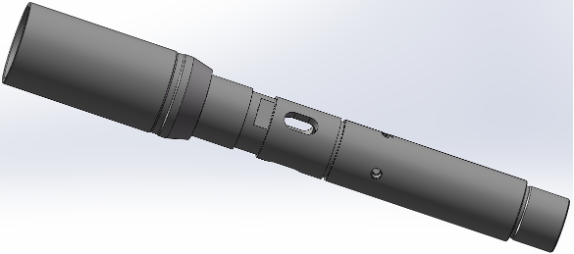
\includegraphics[width=0.4\linewidth]{figure/chapter3/filter-outlet-sub.png}%
        \label{fig:filter_outlet_sub}
    }
    %\hfill
    % 子图 (b)
    \subfloat[滤进接头]{%
        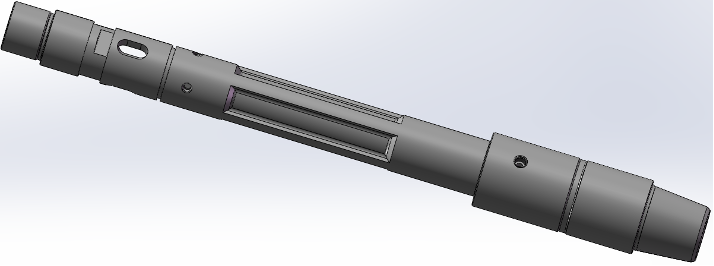
\includegraphics[width=0.5\linewidth]{figure/chapter3/filter-inlet-sub.png}%
        \label{fig:filter_inlet_sub}%
    }
        \caption{过滤工具薄弱零件}
    \label{fig:weak_part_filter}
\end{figure}


\begin{figure}[htbp]
    \centering
    % 子图 (a)
    \subfloat[滤出接头受拉应力分布]{%
        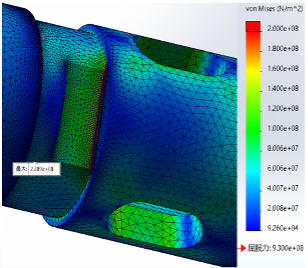
\includegraphics[width=0.45\linewidth]{figure/chapter3/filter-outlet-sub-tensile-stress.png}%
        \label{fig:fea_filter_outlet_tension}
    }
    \hfill
    % 子图 (b)
    \subfloat[滤出接头受扭应力分布]{%
        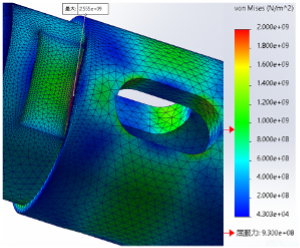
\includegraphics[width=0.45\linewidth]{figure/chapter3/filter-outlet-sub-torsion-stress.png}%
        \label{fig:fea_filter_outlet_torsion}
    }
    \vspace{1em}
      % 子图 (c)
    \subfloat[滤进接头受拉应力分布]{%
        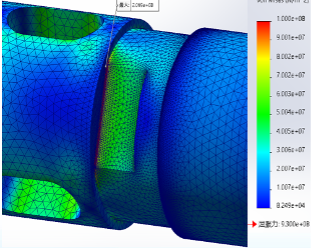
\includegraphics[width=0.45\linewidth]{figure/chapter3/filter-inlet-sub-tensile-stress.png}%
        \label{fig:fea_filter_inlet_tension}
    }
    \hfill
      % 子图 (d)
    \subfloat[滤进接头受扭应力分布]{%
        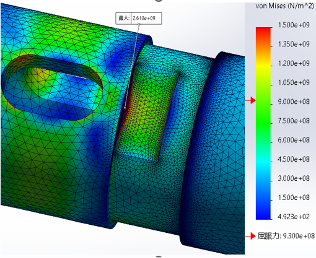
\includegraphics[width=0.45\linewidth]{figure/chapter3/filter-inlet-sub-torsional-stress.png}%
        \label{fig:fea_filter_inlet_torsion}
    }
        \caption{过滤工具薄弱零件受载有限元分析结果}
    \label{fig:weak_part_filter_fea}
\end{figure}


\subsection{过滤容积计算}

过滤工具容量 $V$ 的计算式为：
\begin{equation}
V = L \cdot A = L \cdot \frac{\pi \cdot (D^2 - d^2)}{4} \times 10^{-6}
\end{equation}
式中，$V$---过滤容量，L；

$L$---过滤腔长度，mm；

$A$---过滤腔环形截面积，$\text{mm}^2$；

$D$---大径，mm；

$d$---小径，mm。

代入数值计算得：
\begin{align}
    V &= L \cdot A = L \cdot \frac{\pi \cdot (D^2 - d^2)}{4} \times 10^{-6} \\
      &= 4864.56 \times \frac{\pi \cdot (100.26^2 - 73.03^2)}{4} \times 10^{-6} \\
      &= 18.0\,\text{L} \ge 15\,\text{L}
\end{align}
满足设计要求。

各主要受力件的强度校核结果汇总见表~\ref{tab:force_data_filter}。

\begin{table}[htbp]
    \centering
    \caption{受力件数据统计表}
    \label{tab:force_data_filter}
    \renewcommand{\arraystretch}{1.5} % 增加行高，使表格更美观
    \begin{tabularx}{.9\textwidth}{Xc}
        \toprule % 顶线
        \textbf{受力类型} & \textbf{数据} \\
        \midrule % 栏目线
        材料屈服强度 $\sigma_s$ & $930\,\text{MPa}$ \\
        螺纹最大剪切力 $F_{\max1}$ & $1690.3\,\text{kN}$ \\
        提升短节最大拉力 $F_{\max2}$ & $2838.8\,\text{kN}$ \\
        滤进接头最大拉力 $F_{\max3}$ & $2759.4\,\text{kN}$ \\
        滤出接头最大拉力 $F_{\max4}$ & $2859.0\,\text{kN}$ \\
        下接头最大拉力 $F_{\max5}$ & $2838.8\,\text{kN}$ \\
        材料许用切应力 $[\tau]$ & $620\,\text{MPa}$ \\
        最大扭矩 & $39\,\text{kN}\cdot\text{m}$ \\
        提升短节最大扭力 $T_{\max1}$ & $209.3\,\text{kN}\cdot\text{m}$ \\
        滤进接头最大扭力 $T_{\max2}$ & $77.1\,\text{kN}\cdot\text{m}$ \\
        滤出接头最大扭力 $T_{\max3}$ & $79.3\,\text{kN}\cdot\text{m}$ \\
        下接头最大扭力 $T_{\max4}$ & $136.9\,\text{kN}\cdot\text{m}$ \\
        过滤容量 & $18\,\text{L}$ \\
        \bottomrule % 底线
    \end{tabularx}
\end{table}


\section{操作方式}
\begin{itemize}
	\item 使用时须确保清理盖板处于拧紧状态，避免工具使用中途因清理盖板脱落而导致过滤功能失效。
	\item 清理碎屑时，只需拆卸清理盖板即可，无需拆卸工具本体。
	\item 使用加长版时，需替换过滤套筒、过滤外筒及过滤内筒三个零件，其余零件按原装配方式装配即可。
\end{itemize}


\section{维护与保养}

多功能过滤工具每次使用后，应及时清理收集的碎屑，以免影响下一次工具作业；随后用清水清洗各零件，其中上下扶正套筒及清理盖板处需重点清理。工具在井上多次使用或在恶劣条件下工作后，应进行维护修理：全部拆开并更换所有密封件及易损件，检查螺纹及零件是否有损伤，维修完成后重新装配。

\chapter[可变径刮管工具设计]{可变径刮管工具设计\protect\footnote{合同条款：5.1.3井筒高效清洁关键技术配套工具设计——（4）可变径刮管工具设计}}
	% !TeX root = ../../main.tex
\section{工具总体结构设计}

GGQ95 型可变径套管刮管器用于通过 7\inch 套管后，清除 9-5/8\inch 套管内壁上的残余水泥、泥块、轧制过程中产生的毛刺与鳞片、管内防砂射孔时镶在管壁上的射孔弹、生产井套管上的铁锈与水垢以及硬石蜡等影响正常施工作业的杂物。其结构如图~\ref{fig:variable_scrapter_structure}所示，可变径套管刮削器由上接头、旋转连杆座、连杆、刮刀、芯轴、复位总成、工作活塞、工作弹簧、下接头、节流喷嘴、中间外筒、中间芯轴、激活球座、钢球以及标准件、密封件等零件组成。刮刀采用两组 5 瓣圆周错位排布，覆盖 9-5/8\inch 套管内径圆周 360° 方向。

该工具的工作原理为：投球后激活球座下行，建立活塞腔与工具水眼流道，水眼内的液压力推动工作活塞并迫使工作弹簧上行，在连杆机构的作用下刮刀张开、贴紧套管内壁；随后上提、下放管柱即可实现刮刀对套管内壁的刮削清洁。工具的上下接头分别连接管柱，并通过芯轴连接，可传递扭矩和提拉、下放载荷；旋转连杆座可迫使整组刮刀绕工具自由旋转，当套管内壁变形或通过性较差时，刮刀可绕工具旋转错位通过。该工具的技术参数见表~\ref{tab:ggq95}。

\begin{figure}[htbp]
	\centering
	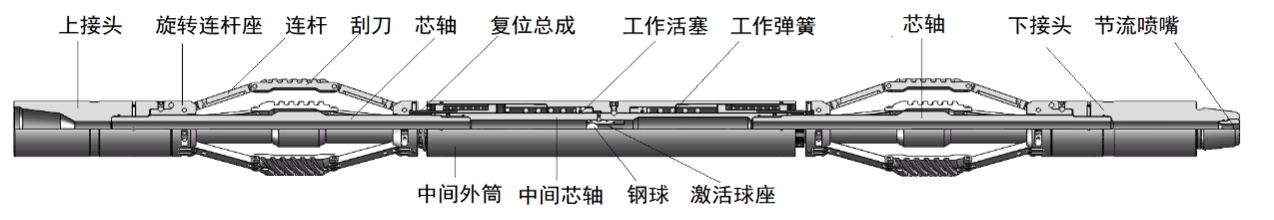
\includegraphics[width=1.\textwidth]{figure/chapter3/part5/variable-scrapter-structure.png}
	\caption{可变径刮管器结构示意图}
	\label{fig:variable_scrapter_structure}
\end{figure}

\begin{table}[htbp]
    \centering
    \caption{GGQ95型可变径套管刮管器技术参数}
    \label{tab:ggq95}
    \renewcommand{\arraystretch}{1.2} % 适当增加行高，提升阅读体验
    \small % 调整整体字号，适应表格宽度
    \begin{tabular}{ccccccc}
        \toprule
        型号 & \begin{tabular}[c]{@{}c@{}}本体最大外径\\(mm)\end{tabular} & \begin{tabular}[c]{@{}c@{}}刮刀收回最小外径\\(mm)\end{tabular} & \begin{tabular}[c]{@{}c@{}}刮刀最大外径\\(mm)\end{tabular} & \begin{tabular}[c]{@{}c@{}}水眼\\(mm)\end{tabular} & \begin{tabular}[c]{@{}c@{}}总长\\(mm)\end{tabular} & \begin{tabular}[c]{@{}c@{}}接头扣\\(API)\end{tabular} \\
        \midrule
        GGQ95 & 140 & 136 & 229+ & 38.1 & 2965 & NC38 \\
        \bottomrule
    \end{tabular}
\end{table}


\section[可变径刮管工具设计计算与校核]{可变径刮管工具设计计算与校核\protect\footnote{合同条款：5.2.1.3井筒高效清洁关键技术配套工具设计——（4）可变径刮管工具：抗拉$>=100\mathrm{T}$，抗扭$>17\,\mathrm{kN}\cdot\mathrm{m}$}}


\subsection{主要受力件的螺纹强度校核}

9-5/8\inch 可变径刮壁器的主要受力件为刮刀芯轴，其主要受力螺纹为 $\mathrm{Tr}\,65 \times 4-8e$，危险截面即位于该螺纹的根部。

螺纹牙的剪切强度按下式计算：
\begin{equation}
	\begin{aligned}
	    F_{\max} &= [\tau] \cdot k_z \cdot \pi \cdot d_1 \cdot b \cdot z \cdot 10^{-3} \\
	    [\tau] &= \frac{\sigma_s}{n}
	\end{aligned}
	\end{equation}
	
式中，$F_{\max}$---工具最大拉力，kN；

$[\tau]$---螺纹牙的许用剪切强度，MPa；

$k_z$---螺纹各圈的载荷不均系数，根据《机械设计手册》螺纹连接（紧固件连接）部分中螺纹牙的剪切强度计算及各圈螺纹载荷分配的规定\cite{ref26}，取 $k_z = 0.56$；

$d_1$---螺纹底径，mm；

$b$---螺纹牙根宽度，mm；

$z$---旋合圈数；

$\sigma_s$---材料最小屈服强度，取 1068 MPa；

$n$---安全系数，根据《机械设计手册》螺纹连接部分中螺纹牙强度校核的安全系数取值规定\cite{ref26}，取 $n = 2.5$。

将 $\mathrm{Tr}\,65 \times 4-8e$ 螺纹的相关参数代入，计算得：
\begin{equation}
    \begin{aligned}
    F_{\max} &= [\tau] \cdot k_z \cdot \pi \cdot d_1 \cdot b \cdot z \cdot 10^{-3} \\
             &= 427.2 \times 0.56 \times 3.14 \times 62 \times 2.6 \times 23.5 \times 10^{-3} \\
             &= 2845.65\,\mathrm{kN} \\
             &> 1000\,\mathrm{kN}
    \end{aligned}
\end{equation}
计算结果表明，螺纹牙的剪切强度满足设计要求。


\subsection{主要受力件的零件抗拉强度校核}

9-5/8\inch 可变径刮壁器的主要受力件为刮刀芯轴和芯轴连接筒，两者的抗拉危险截面分别为刮刀芯轴小螺纹 $\mathrm{Tr}\,65 \times 4-8e$ 螺纹根部和芯轴连接筒内螺纹 $\mathrm{Tr}\,65 \times 4-8H$ 螺纹根部。

抗拉强度按下式计算：
\begin{equation}
    F_{\max} = \frac{\pi \cdot (D^2 - d^2) \cdot \sigma_s}{4 \cdot n} \times 10^{-3}
\end{equation}
式中，$F_{\max}$---工具最大拉力，kN；

$D$---危险截面外径，mm；

$d$---危险截面内径，mm；

$\sigma_s$---材料最小屈服强度，取 1068 MPa；

$n$---安全系数，取 $n = 1.5$。

（1）刮刀芯轴危险截面最大抗拉计算
\begin{equation}
    \begin{aligned}
    F_{\max} &= \frac{\pi \cdot (D^2 - d^2) \cdot \sigma_s}{4 \cdot n} \times 10^{-3}
             = \frac{3.14 \times (62^2 - 38.1^2) \times 1068}{4 \times 1.5} \times 10^{-3} \\
             &= 1337.15\,\mathrm{kN} > 1000\,\mathrm{kN}
    \end{aligned}
\end{equation}
满足设计要求。

（2）芯轴连接筒危险截面最大抗拉计算
\begin{equation}
    \begin{aligned}
    F_{\max} &= \frac{\pi \cdot (D^2 - d^2) \cdot \sigma_s}{4 \cdot n} \times 10^{-3}
             = \frac{3.14 \times (80^2 - 66^2) \times 1068}{4 \times 1.5} \times 10^{-3} \\
             &= 1142.43\,\mathrm{kN} > 1000\,\mathrm{kN}
    \end{aligned}
\end{equation}
满足设计要求。


\subsection{主要受力件的零件抗扭强度校核}

9-5/8\inch 可变径刮壁器的主要受力件为刮刀芯轴和芯轴连接筒，其抗扭危险截面与抗拉校核相同，分别位于刮刀芯轴小螺纹 $\mathrm{Tr}\,65 \times 4-8e$ 螺纹根部和芯轴连接筒内螺纹 $\mathrm{Tr}\,65 \times 4-8H$ 螺纹根部。

抗扭强度按下式计算：
\begin{align}
    \tau &= \frac{16 \cdot D \cdot T_{\max}}{\pi \cdot (D^4 - d^4)} \times 10^{6} \\
    T_{\max} &= \frac{[\tau] \cdot \pi \cdot (D^4 - d^4)}{16 \cdot D} \times 10^{-6} \\
    [\tau] &= n \cdot \sigma_s = 0.66 \times 1068\,\mathrm{MPa} = 704.88\,\mathrm{MPa}
\end{align}
式中，$T_{\max}$---工具最大扭矩，$\mathrm{kN}\cdot\mathrm{m}$；

$\tau$---危险截面的切应力，MPa；

$[\tau]$---材料许用切应力，MPa；

$\sigma_s$---材料屈服强度，MPa；

$D$---危险截面外径，mm；

$d$---危险截面内径，mm；

$n$---许用切应力与许用拉应力之比，根据《机械设计手册》零件强度校核中许用应力折减系数的取值规定\cite{ref26}，取 $n = 0.66$。

（1）刮刀芯轴危险截面最大抗扭计算
\begin{equation}
    \begin{aligned}
    T_{\max} &= \frac{[\tau] \cdot \pi \cdot (D^4 - d^4)}{16 \cdot D} \times 10^{-6}
             = \frac{704.88 \times 3.14 \times (62^4 - 38.1^4)}{16 \times 62} \times 10^{-6} \\
             &= 28.27\,\mathrm{kN}\cdot\mathrm{m} > 17\,\mathrm{kN}\cdot\mathrm{m}
\end{aligned}
\end{equation}
满足设计要求。

（2）芯轴连接筒危险截面最大抗扭计算
\begin{equation}
    \begin{aligned}
    T_{\max} &= \frac{[\tau] \cdot \pi \cdot (D^4 - d^4)}{16 \cdot D} \times 10^{-6}
             = \frac{704.88 \times 3.14 \times (80^4 - 66^4)}{16 \times 80} \times 10^{-6} \\
             &= 38.02\,\mathrm{kN}\cdot\mathrm{m} > 17\,\mathrm{kN}\cdot\mathrm{m}
\end{aligned}
\end{equation}
满足设计要求。


\subsection{球座剪钉剪切力与节流泵压计算}

9-5/8\inch 可变径刮壁器需要投球后憋压将球座剪钉剪断，迫使球座下移建立压力通道才能开始工作，因此剪钉的剪断力和投球后球座处的憋压压力是激活工具的重要参数。

刮壁器的球座圆周设计 3 组剪钉参与剪切，剪钉选用 45 号非调质料制作，则工具激活所需的推力为：
\begin{equation}
    \begin{aligned}
        F_s \ge [\tau] \cdot A = 0.8 \times [\sigma] \times 3 \times (\pi \cdot R^2) &= 0.8 \times 450 \times 3 \times 3.14 \times 4^2 \\
        &= 54259.2\,\mathrm{N}
    \end{aligned}
\end{equation}
式中，$F_s$---工具激活所需的最小推力，N；

$[\tau]$---材料许用剪应力，塑性材料取 $0.6[\sigma]$、脆性材料取 $0.8[\sigma]$；

$A$---单个剪钉的剪切面积，$\mathrm{mm}^2$；

$R$---单个剪钉的半径，mm。

刮壁器投入钢球后球座流道被堵塞，井口泵压直接作用在球座上，根据上述计算所得的最小推力 $F_s$，可计算出激活工具所需的最小泵压 $P_0$：
\begin{equation}
    P_0 \ge \frac{F_s}{A_q} = \frac{F_s}{\pi \cdot \left(\frac{d}{2}\right)^2} = \frac{54259.2}{3.14 \times \left(\frac{45}{2}\right)^2} = 34.12\,\mathrm{MPa}
\end{equation}
式中，$P_0$---激活工具所需的最小泵压，MPa；

$A_q$---球座承压面积，$\mathrm{mm}^2$；

$d$---球座承压面直径，取 45 mm。

计算表明，当泵压不小于 $34.12\,\mathrm{MPa}$ 时，工具可以被激活。


\subsection{节流喷嘴的尺寸和节流压力关系}

刮壁器激活后流道建立，工具底部的节流喷嘴形成的节流压差为工具提供工作压力 $\Delta P \le 4\,\mathrm{MPa}$，故需要计算节流喷嘴的尺寸与节流压力的关系。

由公式：
\begin{equation}
    \Delta P \le \frac{827 \cdot \rho \cdot Q^2}{C^2 \cdot d_e^4}
\end{equation}

推算喷嘴最小直径为：
\begin{equation}
    d_e \ge \sqrt[4]{\frac{827 \cdot \rho \cdot Q^2}{C^2 \cdot \Delta P}} = \sqrt[4]{\frac{827 \times 1.1 \times 40^2}{0.96^2 \times 4}} = 25.06\,\mathrm{mm}
\end{equation}
式中，$d_e$---喷嘴节流孔最小直径，mm；

$\Delta P$---刮壁器最大节流压力（即最大节流工作压差），MPa；

$\rho$---钻井液密度，$1.1\,\mathrm{g/cm^3}$；

$Q$---工作时泵排量，暂定值为 $40\,\mathrm{L/s}$；

$C$---流量系数，无因次，取 $0.95 \sim 0.98$。


\subsection{连杆销抗剪切强度计算}

9-5/8\inch 可变径刮壁器在激活后的工作过程中，刮壁作业所承受的冲击载荷由连杆铰链销承受，故有必要计算连杆销的抗剪切强度。假定刮壁器作业时受到的最大轴向力为工具最大抗拉力，即 $F_{\max} = 1000\,\mathrm{kN}$；销钉材料选用 M35 热后料，$[\sigma] \ge 1300\,\mathrm{MPa}$；销钉设计最小直径为：

由切应力公式
\begin{equation}
    \tau = \frac{F_{\max}}{A} = \frac{F_{\max}}{20 \cdot A_0} = \frac{F_{\max}}{\pi \cdot 20 \cdot \left(\frac{d}{2}\right)^2} \le [\tau]
\end{equation}
式中，$[\tau]$---材料许用剪应力，MPa，塑性材料取 $0.6[\sigma]$、脆性材料取 $0.8[\sigma]$，本例取 $1040\,\mathrm{MPa}$；

$A$---单个连杆销的总剪切面积，每个连杆销有两个剪切面积，故 $A = 2 \times 2A_0 \times 5$；

$d$---连杆销的最小直径，mm。

可得
\begin{equation}
    d \ge 2\sqrt{\frac{F_{\max}}{20 \cdot \pi \cdot [\tau]}} = 2\sqrt{\frac{1.0 \times 10^{6}}{20 \times 3.14 \times 1040}} = 7.825\,\mathrm{mm}
\end{equation}

设计连杆销直径 $d = 8\,\mathrm{mm}$，满足设计要求。


\subsection{主要受力件仿真校核}

主要受力件为刮刀芯轴和芯轴连接筒，危险截面出现在螺纹根部，有限元仿真结果如图~\ref{fig:FEA_inner_pipe_variable}所示。刮刀芯轴的最大拉应力为 850 MPa，小于设计要求；最大切应力为 1600 MPa，出现在变径处，但范围极小，属于应力集中导致的局部小尺度高应力，不会引发整体塑性变形，强度满足设计要求。

\begin{figure}[htbp]
	\centering
	\subfloat[可变径刮管器心轴]{%
	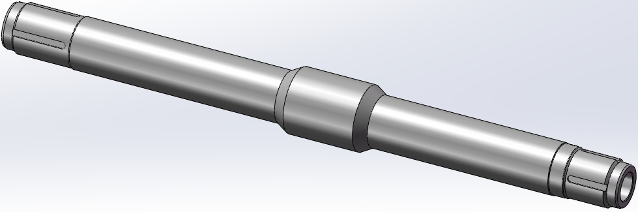
\includegraphics[width=0.7\textwidth]{figure/chapter3/part5/inner-pipe.png}
	}
	\hfill
	\subfloat[抗拉强度分析]{%
	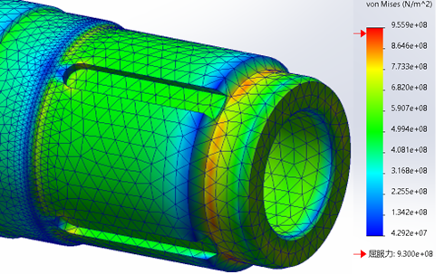
\includegraphics[width=0.4\textwidth]{figure/chapter3/part5/tensile-strength.png}
	}
	\vspace{1em}
	\subfloat[抗扭强度分析]{%
	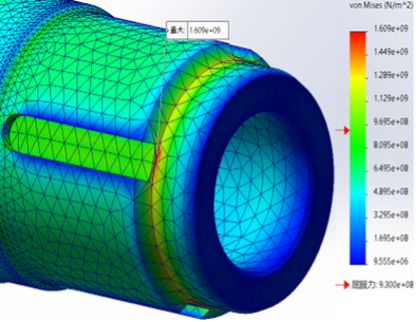
\includegraphics[width=0.3\textwidth]{figure/chapter3/part5/torsional-strength.png}
	}
	\caption{可变径刮管工具薄弱零件强度有限元分析}
	\label{fig:FEA_inner_pipe_variable}
\end{figure}


\section{拆装步骤}

工具入井后到达管子站进行保养前，需冲洗外表面，并准备好内六角扳手、起子、扳手等拆卸工具。

(1) 工具冲洗干净后，将上、下接头的 M16 螺钉拆卸，取出内部的防掉钢珠；取出下接头喷嘴；如下图箭头所示位置。

\begin{figure}[H]
\centering
	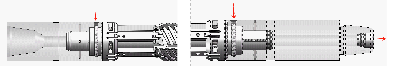
\includegraphics[width=1.\textwidth]{figure/chapter3/part5/unsetup/ball.png}
\end{figure}

(2) 拆卸上、下接头的防松螺钉后，分别反转拆卸上、下接头；如下图所示位置。

\begin{figure}[H]
\centering
	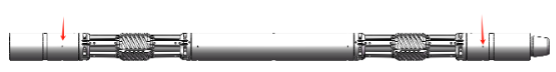
\includegraphics[width=1.\textwidth]{figure/chapter3/part5/unsetup/unsetup-satefy-screw.png}
	\vspace{1em}
	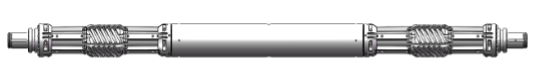
\includegraphics[width=1.\textwidth]{figure/chapter3/part5/unsetup/unsetup-two-subs.png}
\end{figure}

(3) 用起子、扳手取下连杆座、连杆、刮刀等之间的铰链销、防掉螺钉等标准件后，依次拆卸旋转连杆座、连杆、刮刀等零件；如下图所示。

\begin{figure}[H]
\centering
	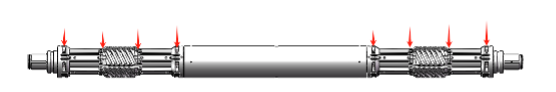
\includegraphics[width=1.\textwidth]{figure/chapter3/part5/unsetup/unsetup-fasten-parts.png}
\end{figure}

(4) 拆卸各部位的锁紧螺钉、铰链销、防掉螺钉等零件。

(5) 拆卸两头的旋转连杆座。

\begin{figure}[H]
\centering
	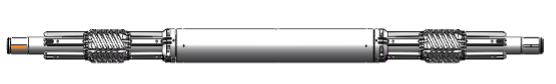
\includegraphics[width=1.\textwidth]{figure/chapter3/part5/unsetup/rotary-lever-set.png}
\end{figure}

(6) 拆卸两头的连杆、刮刀等零件。

\begin{figure}[H]
\centering
	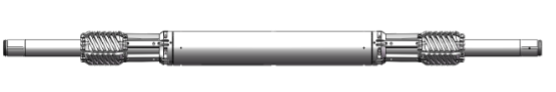
\includegraphics[width=1.\textwidth]{figure/chapter3/part5/unsetup/end-links.png}
	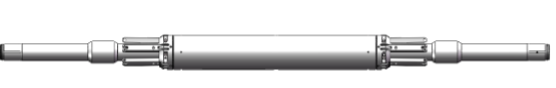
\includegraphics[width=1.\textwidth]{figure/chapter3/part5/unsetup/unsetup-scraper.png}
	
\includegraphics[width=1.\textwidth]{figure/chapter3/part5/unsetup/left-links.png}
\end{figure}

(7) 分别反转拆卸两头的芯轴，从下部取出激活球座和钢球，如下图所示。

\begin{figure}[H]
\centering
	
\includegraphics[width=1.\textwidth]{figure/chapter3/part5/unsetup/unsetup-inner-pipe.png}
	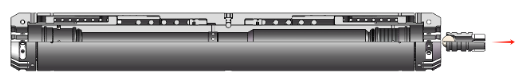
\includegraphics[width=1.\textwidth]{figure/chapter3/part5/unsetup/unsetup-ball-and-seat.png}
\end{figure}

(8) 夹紧中间外筒方向旋转复位总成，分别取出上、下两头的复位总成，然后依次对复位总成进行拆解，如下图所示。

\begin{figure}[H]
\centering
	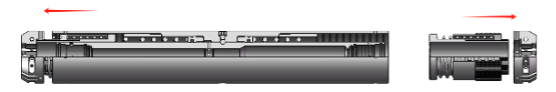
\includegraphics[width=1.\textwidth]{figure/chapter3/part5/unsetup/reseting-assembly.png}
	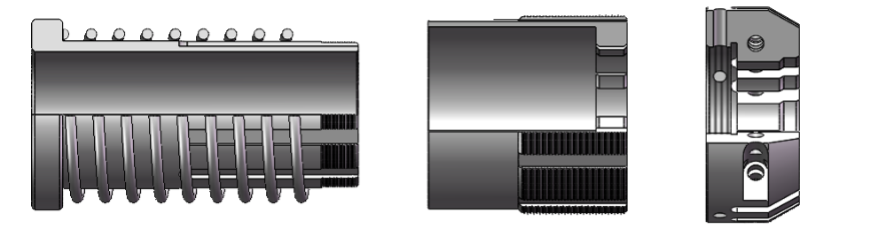
\includegraphics[width=1.\textwidth]{figure/chapter3/part5/unsetup/resetting-assembly-unsetup.png}
\end{figure}

(9) 取出中间筒体和中间芯轴的限位钢球，随后取下中间芯轴、弹簧、活塞、活塞限位套等零件；最后拆卸各零件上的密封圈，即拆卸完毕。

(10) 拆卸中间筒体和中间芯轴的钢球堵和限位钢球。

\begin{figure}[H]
\centering
	
\includegraphics[width=1.\textwidth]{figure/chapter3/part5/unsetup/middle-body-inner-pipe-ball.png}
\end{figure}

(11) 拆卸中间芯轴，固定中间筒体后从任意一头抽出中间芯轴即可。

\begin{figure}[H]
\centering
	
\includegraphics[width=1.\textwidth]{figure/chapter3/part5/unsetup/middle-inner-pipe-unsetup.png}
\end{figure}

(12) 按下图所示方向，分别从两头拆卸活塞、工作弹簧、活塞限位套等零件。

\begin{figure}[H]
\centering
	
\includegraphics[width=1.\textwidth]{figure/chapter3/part5/unsetup/piston-spring-limiter.png}
\end{figure}

(13) 装配步骤与拆卸步骤相反，装配过程中需要注意不要损伤密封面、螺纹牙形等配合处，密封面和螺纹组装前要求涂抹润滑油。

工具的易损件及配件清单见表~\ref{tab:parts_list}。

\begin{table}[htbp]
    \centering
    \caption{易损件及配件清单表}
    \label{tab:parts_list}
    \small % 代号较长，缩小字号以适应表格宽度
    \setlength{\tabcolsep}{4pt} % 减小列间距，避免超出正文版心
    \renewcommand{\arraystretch}{1.5} % 调整行间距，使表格不拥挤
    \begin{tabular}{cccc}
        \toprule
        \textbf{序号} & \textbf{代号} & \textbf{名称} & \textbf{单套数量} \\
        \midrule
        1  & 2-223 PAEKE FKM                      & O 形圈                 & 1   \\
        2  & GB/T308-2002 $\phi 30$               & 钢球 30                & 1   \\
        3  & ON 0800 052 00110 D （PARKE）        & 双作用格莱圈           & 2   \\
        4  & 2-243 PAEKE FKM                      & O 形圈                 & 2   \\
        5  & 2-222 PAEKE FKM                      & O 形圈                 & 2   \\
        6  & 2-229 PAEKE FKM                      & O 形圈                 & 2   \\
        7  & 2-140 PAEKE FKM                      & O 形圈                 & 2   \\
        8  & 2.62$\times$62 GB/T1235                     & O 形圈                 & 2   \\
        9  & GB/T 77-2007                         & 内六角平端紧定螺钉 M8$\times$20  & 10  \\
        10 & GB/T 80-2007                         & 内六角凹端紧定螺钉 M8$\times$30  & 8   \\
        11 & GB/T 80-2007                         & 内六角凹端紧定螺钉 M8$\times$10  & 8   \\
        12 & GB/T 79-2007                         & 内六角圆柱端紧定螺钉 M10$\times$30 & 10  \\
        13 & GB/T 77-2007                         & 内六角平端紧定螺钉 M8$\times$8   & 8   \\
        14 & $\phi 25$ 喷嘴                       & 节流喷嘴               & 1   \\
        15 & G98Cr18 12 G40 $\pm 0$ GB/T 308      & $\phi 12$ 钢球         & 100 \\
        16 & GB/T 80-2007                         & 内六角凹端紧定螺钉 M5$\times$12  & 40  \\
        17 & GB/T 77-2007                         & 内六角平端紧定螺钉 M16$\times$16 & 2   \\
        18 & GB/T 77-2007                         & 内六角平端紧定螺钉 M10$\times$35 & 20  \\
        19 & GGQ95-19                             & 工作弹簧               & 2   \\
        20 & GGQ95-18                             & 复位弹簧               & 2   \\
        21 & GGQ95-17                             & 密封堵                 & 2   \\
        22 & GGQ95-16                             & 丝堵                   & 2   \\
        23 & GGQ95-7                              & 刮刀铰链销             & 20  \\
        24 & GGQ95-6                              & 59BPF 刮刀             & 10  \\
        25 & GGQ95-5                              & 活动铰链销             & 20  \\
        \bottomrule
    \end{tabular}
\end{table}


\section{操作方式}

\subsection{下井前准备}
\begin{itemize}
	\item 了解井况，确定套管规格和深度等基本信息；
	\item 选配适合套管规格的刮刀；
	\item 本可变径刮管器应与 7\inch 及以上其它刮管器配合使用；
	\item 确定刮管工艺，了解泵压和排量，并根据图~\ref{fig:pressure_decrease_with_Q_size}所示不同排量下喷嘴尺寸与压降的关系选装合适的喷嘴及剪钉。
\end{itemize}

\begin{figure}[htbp]
	\centering
	\subfloat[10L/s]{%
	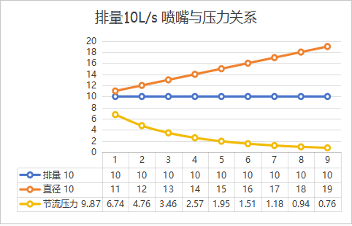
\includegraphics[width=0.4\textwidth]{figure/chapter3/part5/10LperSec.png}
	}
	%\hfill
	\subfloat[20L/s]{%
	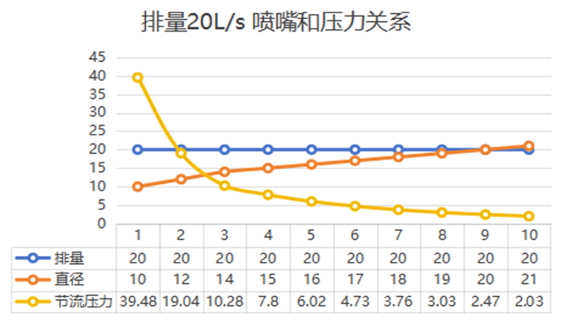
\includegraphics[width=0.4\textwidth]{figure/chapter3/part5/20LperSec.png}
	}
	\vspace{1em}
	\subfloat[30L/s]{%
	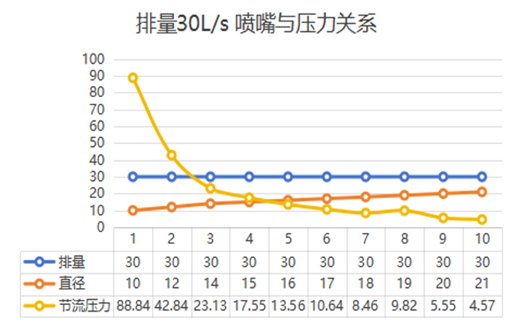
\includegraphics[width=0.4\textwidth]{figure/chapter3/part5/30LperSec.png}
	}
	\subfloat[40L/s]{%
	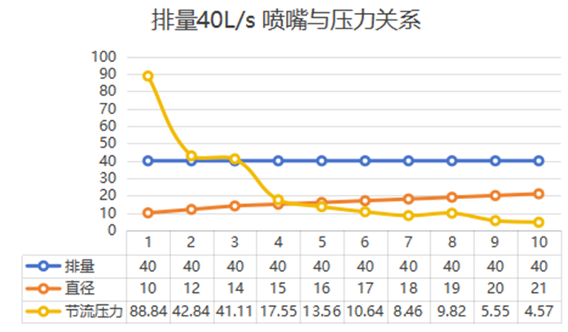
\includegraphics[width=0.4\textwidth]{figure/chapter3/part5/40LperSec.png}
	}
	\caption{喷嘴压降与排量、喷嘴尺寸之间的关系}
	\label{fig:pressure_decrease_with_Q_size}
\end{figure}

\subsection{操作}
\begin{itemize}
	\item 下井前按照作业要求依次连接好管柱，刮管器前端需接与套管规格对应的扶正器；推荐管柱组合为：通井钻头 $+$ 扶正器 $+$ 7\inch 刮管器 $+$ 可变径刮管器 $+$（选装其它套管清洁工具）$+$ 上部钻柱。
	\item 接上可变径刮管器后，夹紧下接头、大钳打上接头，拧紧刮管器各螺纹，井口以开泵压力 $\le 20 \pm 5\,\mathrm{MPa}$、排量 $\le 10\,\mathrm{L/s}$ 进行试循环，时间 $1 \sim 5\,\mathrm{min}$。
	\item 待循环正常并确定刮刀未弹出本体后，慢慢旋转下放工具，并进行其它钻磨、完井、试油、测试、刮小规格套管等作业。
	\item 当小规格套管刮管作业完成后，将可变径刮管器提升至 9-5/8\inch 套管所需的井深位置，投入钢球，开泵打压激活刮刀张开，启动作业；
	\item 刮管器打开压力 $=$ 静液柱压力 $+$ 泵压（绝对压力），即泵压 $\ge$ 绝对压力 $-$ 静液柱压力。
	\item 激活判定：投入钢球后观察泵压，若泵压上升过程中突然下降，说明可变径刮管器已启动；随后停泵，按工具入井前选定的喷嘴尺寸所要求的泵压和排量稳定循环，同时通过上提、下放工具进行 9-5/8\inch 套管的刮管作业。
	\item 刮管作业时观察指重表无任何显示，即下放悬重不降、上提悬重不升，表明已刮削干净。
\end{itemize}

\subsection{注意事项}
\begin{itemize}
	\item 工具与管柱的连接扣必须拧紧。
	\item 两组刮刀的螺旋升角应保持同方向。
	\item 可变径刮管器在下井过程中如遇阻，应慢慢旋转几圈后再下放。
	\item 刮管作业过程中，必须始终保持钻井液循环畅通。
\end{itemize}

\section{维护与保养}
\begin{itemize}
	\item 出井后应清洗干净，并检查各零件，如弹簧失效必须更换。各螺纹涂螺纹脂，各零件涂油，存放在阴干处。
	\item 每次作业后，都应将工具完全拆开并清洗，更换所有 O 形圈和损坏的弹簧，检查刮管器本体上的内套是否粘接牢固。用肉眼检查所有的密封面和接头丝扣是否损坏，若发现有损坏的零件都应更换，这些损坏的零件对工具的可靠性会产生不利的影响。
	\item 在拆卸、保养前，应准备好正确、有效的装配图和工具保养维护说明书及工具维护保养单。
	\item 对高温井作业以及有酸及硫化氢存在的修井作业，应提前更换相应耐腐蚀、耐高温的密封件和配件。
	\item 有关该工具使用和维护保养的其他任何问题，请与我校联系。
\end{itemize}



\section{清洁工具组合工艺}

根据不同井况需求进行清洁工具组合，减少下钻趟数，提高作业效率。9-5/8\inch 井筒深度清洁作业中，常用的管柱组合（自上而下）如下，实际作业时可根据井况要求进行调整与扩展：

（1）钻杆 $+$ 震击器 $+$ 钻杆 $+$ 9-5/8\inch 多功能过滤工具 $+$ 短钻杆 $+$ “四合一”集成式井筒清洁工具 $+$ 短钻杆 $+$ 浮阀 $+$ 钻头；

（2）钻杆 $+$ 震击器 $+$ 钻杆 $+$ 9-5/8\inch 多功能过滤工具 $+$ 短钻杆 $+$ “四合一”集成式井筒清洁工具 $+$ 循环洗井阀 $+$ 短钻杆 $+$ “三合一”集成式井筒清洁工具；

（3）钻杆 $+$ 震击器 $+$ 钻杆 $+$ 9-5/8\inch 多功能过滤工具 $+$ 短钻杆 $+$ “四合一”集成式井筒清洁工具 $+$ 循环洗井阀 $+$ 短钻杆 $+$ 可变径刮管工具。


%\section{本章小结}
%
%针对连续砂床、严重出砂井况下常规水力冲砂效率低、除砂效果差，以及套管内壁结垢、铁磁性碎屑残留、缩径与变径等井筒清洁难题，本章按照“冲—刮—刷—吸—滤—通”多功能协同的思路，完成了“三合一”脉冲式冲刮刷集成式井筒清洁工具、“四合一”通刮刷磁集成式井筒清洁工具、大容量强磁吸附工具、多功能过滤工具和可变径刮管工具共五类工具的结构设计、理论计算、仿真校核与使用维护研究，主要结论如下：
%
%（1）“三合一”脉冲式冲刮刷集成式井筒清洁工具。
%
%结构上由脉冲发生模块与旋转喷头模块构成，并配置毛刷刮管模块。旋转喷头模块利用两组偏心夹角喷嘴射流产生的反冲力矩驱动喷头自转，实现套管内壁 360° 无死角的周向冲洗；脉冲发生模块通过活塞—矩形弹簧机构把地面泵注的稳态液流转化为高、负压交替的低频水力脉冲波，其轴向机械振荡与径向水力冲击相叠加，可破坏压实砂床的结构、为环空砂砾补充扰动动能，抑制砂砾再沉积。
%	
%针对工具内部流体压力与机械部件的耦合机制，基于连续性方程与牛顿运动定律建立了包含蓄能、开启、喷射与复位四个阶段的非线性常微分方程组，形成了脉冲发生模块的瞬态动力学模型。在典型工况（$Q=50\mathrm{m^3/h}$、$K=757176\mathrm{N/m}$、侧向出水孔高度 $l_1=75\mathrm{mm}$）下，活塞最大冲程为 $88.13\mathrm{mm}$，单次工作周期为 $12.86\mathrm{ms}$，对应工作频率为 $77.76\mathrm{Hz}$。
%	
%参数影响规律表明：输入排量是决定脉冲特性的首要参数，在 $46\sim58\mathrm{m^3/h}$ 的设计区间内，活塞最大冲程随排量近似线性增长，正向速度峰值由 $14.5\mathrm{m/s}$ 增至 $23.1\mathrm{m/s}$，工作频率随排量提高而非线性增大；矩形弹簧刚度增大使活塞冲程阶梯式下降、单次循环时间缩短、工作频率升高；侧向出水孔高度增大则蓄能阶段延长、工作频率降低、开孔有效余量减小。设计时需在冲程与频率之间取得平衡，并保证适宜的开孔有效余量。
%
%强度校核方面，脉冲器危险截面（螺纹应力分散槽处）的许用拉力为 $690.8\mathrm{kN}$，大于 $400\mathrm{kN}$ 的设计要求；许用扭矩为 $11.74\mathrm{kN\cdot m}$，大于 $8\mathrm{kN\cdot m}$ 的设计要求；脉冲器心轴的最大拉应力为 $630\mathrm{MPa}$，小于设计要求，最大切应力为 $994\mathrm{MPa}$，但范围极小，属应力集中引起的局部小尺度高应力，不会引发整体塑性变形。
%	
%冲洗效果方面，Fluent 欧拉多相流仿真表明，使用该工具后井筒内砂砾质量较无工具对照组降低了 19\%，喷嘴截面下方环空冲砂液轴向流速明显高于传统刚性钻杆，砂砾不再沉积于环空底部而富集于环空两侧，竖直截面上砂床前缘由距入口 $0.8\mathrm{m}$ 推进至压力出口，说明该工具能有效抑制砂砾在工具处的沉积并显著提升携砂与清砂效率；喷头流动仿真表明，射流冲击压力先使污染物破裂松动，随后持续的剪切应力把松动的污染物卷吸进入主流，其中低频脉动负责大块污垢的宏观剥离、高频脉动负责残留微粒的清除，因此实际应用中应根据污垢特性（硬度、厚度、黏附性）调整脉冲频谱，必要时采用复合频率策略。
%
%
%（2）“四合一”通刮刷磁集成式井筒清洁工具。该工具集通井扶正、机械刮削、刷洗清扫与强磁吸附（“通、刮、刷、磁”）四项功能于一体，采用长轴式模块化布局，形成 7\inch、9-5/8\inch、13-3/8\inch 三种规格，刮刀、毛刷与磁吸模块可根据井况选装组合；刮刀采用弹簧浮动加载与可更换齿形刀片，遇顽固坚硬杂物时扭曲弹簧可压缩储能并在越障后释放，起到缓冲保护作用。校核结果表明：7\inch 规格心轴上 $2.75''\text{-}8$ Stub ACME 连接螺纹的抗拉能力为 $2851.13\mathrm{kN}$，心轴两个危险截面（内、外螺纹根部）的抗拉能力分别为 $1406.08\mathrm{kN}$ 与 $1624.30\mathrm{kN}$，均大于 $1000\mathrm{kN}$ 的抗拉设计指标；心轴两个危险截面的抗扭能力分别为 $31.63\mathrm{kN\cdot m}$ 与 $59.39\mathrm{kN\cdot m}$，端面键的抗扭能力为 $26.53\mathrm{kN\cdot m}$，均大于 $17\mathrm{kN\cdot m}$ 的抗扭设计指标。刮板刮削效果评价试验表明，所设计的刮板能以脆性崩碎的方式有效刮除重晶石/钡锶类硬垢，刮痕深度随弹簧压缩量的增大呈“先较快增加、后趋于饱和”的非线性响应，弹簧预紧力存在最优工作区间；工程应用中应结合套管实际内径匹配刮刀外径与弹簧预紧量，避免盲目增大预紧力，并配合循环冲洗及时排屑，以延缓刀齿堵塞、延长刮板的使用寿命。
%
%（3）大容量强磁吸附工具。工具采用上部（侧吸、带窗保护管，适于吸附小尺度铁质颗粒）与下部（环吸、开放式，适于吸附大尺度铁质碎屑）双强磁结构组合，实现了沿沟槽方向与沿圆周方向的多方向、多尺寸磁性碎屑吸附，永磁块可单独更换、装配数量可按碎屑含量调节，吸附容量可调。经计算，7\inch、17lb/ft 套管下单根工具的吸附容量为 $28.26\mathrm{L}$，两根工具组合后的吸附容量为 $56.52\mathrm{L}$，大于 $50\mathrm{L}$ 的吸附容量设计要求；主要受力件的螺纹强度、抗拉与抗扭强度均满足设计要求，下接头防退扣根部最大剪应力为 $1030\mathrm{MPa}$，略高于屈服强度，属应力集中引起的局部小尺度高应力，不会引发整体塑性变形。永磁材料选型方面，考虑本项目 $150^\circ\mathrm{C}$ 的温度设计指标，对比钐钴（SmCo5）与钕铁硼（N45UH）等材料的退磁曲线后，确定选用耐温性与抗退磁能力更好的钐钴材料；基于 ANSYS Maxwell 的仿真研究表明，上部结构宜采用径向充磁、下部结构宜采用周向（交叉径向）充磁，以获得均匀且最大的表面磁场分布，骨架材料应选用导磁效果好、可磁化程度高的金属合金以聚集磁感线、增大磁通（采用铝制骨架时，永磁体表面磁场由 $0.7\sim1.5\mathrm{T}$ 降至 $0.3\sim0.7\mathrm{T}$，骨架沟槽表面由 $1.2\sim3.5\mathrm{T}$ 降至 $0.2\sim0.4\mathrm{T}$）。此外，从居里温度、工作温度、外部磁场、时间、机械冲击与化学侵蚀六个方面分析了永磁体的退磁影响因素，并结合工具设计给出了磁路闭合存储、不锈钢保护套防护、磁体镀镍防腐、安装规范防划伤等防退磁措施，以及强磁工具的操作方式与维护保养要求。
%
%（4）多功能过滤工具。完成了工具总体结构设计，以及主要受力件的螺纹强度、零件强度与抗扭强度的解析校核和有限元复核：滤出接头最大拉应力为 $238\mathrm{MPa}$、滤进接头最大拉应力为 $206\mathrm{MPa}$，均远小于设计要求；变径处的最大切应力范围极小，属应力集中引起的局部小尺度高应力，不会引发整体塑性变形。过滤容积计算值为 $18.0\mathrm{L}$，满足设计要求；同时给出了以清理盖板为核心的清理操作方式与拆洗维护要求。
%
%（5）可变径刮管工具。完成了主要受力件的螺纹强度、零件抗拉与抗扭强度校核以及刮刀芯轴、芯轴连接筒的有限元仿真校核（刮刀芯轴最大拉应力为 $850\mathrm{MPa}$，小于设计要求），并计算了工具激活与节流的关键参数：球座剪钉的剪切力为 $54259.2\mathrm{N}$，对应的最小激活泵压为 $34.12\mathrm{MPa}$，节流喷嘴的最小直径为 $25.06\mathrm{mm}$（对应节流工作压差不超过 $4\mathrm{MPa}$），连杆销设计直径为 $8\mathrm{mm}$，大于计算所需的 $7.825\mathrm{mm}$；此外给出了拆装步骤、下井前准备、作业操作与注意事项（如以投球后泵压先升后降判断工具启动，以指重表无显示作为刮削干净的判据），以及维护保养规程。
%
%（6）五类工具的配套使用。三合一工具集脉冲发生、旋转喷头与毛刷刮管模块于一体，适用于冲砂洗井及套管内壁清洁；四合一工具兼具通井扶正、刮削、刷洗与磁吸功能；大容量强磁吸附工具、多功能过滤工具与可变径刮管工具既可单独使用，也可与 ZKG 模块化多合一套管清洁工具配套组合使用，从而在同一趟作业中完成通井、刮削、刷洗、铁磁性碎屑吸附与碎屑过滤收集等多项功能，减少起下钻次数。各类工具主要受力件的应力、抗拉与抗扭能力，以及吸附容量、过滤容积等功能指标，均通过理论计算或仿真校核并满足设计要求，且均配套了拆装、操作与维护保养规程，形成了“结构设计—理论计算—仿真校核—使用维护”的完整设计链条。
%
%综上，本章所设计的五类井筒清洁工具在功能上覆盖了砂床破坏、机械刮削、刷洗清扫、强磁吸附、碎屑过滤与变径通井等井筒清洁需求，在强度与功能指标上均通过了计算与仿真校核，为下一步的室内性能试验与现场应用验证奠定了基础。

	
% !TeX root = ../main.tex
% === 【修改】GB/T 7714-2015 参考文献 ===
\clearpage % 参考文献另起一页
\addcontentsline{toc}{chapter}{参考文献} % 将参考文献加入目录

% \bibliographystyle{gbt7714-numerical} % 已由 gbt7714 宏包([numbers])在 \begin{document} 时自动写入，重复声明会使 bibtex 报 "Illegal, another \bibstyle command"
\begin{thebibliography}{99}


\bibitem{ref26} % 机械设计手册（螺纹连接强度校核取值依据）
成大先. 机械设计手册[M]. 第六版. 北京: 化学工业出版社, 2016.

\end{thebibliography}






	
\end{document}